% ******************************* PhD Thesis Template **************************
% Please have a look at the README.md file for info on how to use the template

\documentclass[a4paper,12pt,default,print,index,authoryear]
		{classes/PhDThesisPSnPDF} %final version

%\documentclass[a4paper,12pt,default,draft,index,authoryear]
%{classes/PhDThesisPSnPDF} % draft mode

%\documentclass[a4paper,12pt,times,chapter,index,authoryear]
%{classes/PhDThesisPSnPDF} % chapter mode


% ******************************************************************************
% ******************************* Class Options ********************************
% *********************** See README for more details **************************
% ******************************************************************************

% `a4paper'(The University of Cambridge PhD thesis guidelines recommends a page
% size a4 - default option) or `a5paper': A5 Paper size is also allowed as per
% the Cambridge University Engineering Deparment guidelines for PhD thesis
%
% `11pt' or `12pt'(default): Font Size 10pt is NOT recommended by the University
% guidelines
%
% `oneside' or `twoside'(default): Printing double side (twoside) or single
% side.
%
% `print': Use `print' for print version with appropriate margins and page
% layout. Leaving the options field blank will activate Online version.
%
% `index': For index at the end of the thesis
%
% `draftclassic': For draft mode without loading any images 
% (same as draft in book)
%
% `draft': Special draft mode with line numbers, images, and water mark with
% timestamp and custom text. Position of the text can also be modified.
%
% `abstract': To generate only the title page and abstract page with
% dissertation title and name, to submit to the Student Registry
%
% `chapter`: This option enables only the specified chapter and it's references
%  Useful for review and corrections.
%
% ************************* Custom Page Margins ********************************
%
% `custommargin`: Use `custommargin' in options to activate custom page margins,
% which can be defined in the preamble.tex. Custom margin will override
% print/online margin setup.
%
% *********************** Choosing the Fonts in Class Options ******************
%
% `times' : Times font with math support. (The Cambridge University guidelines
% recommend using times)
%
% `fourier': Utopia Font with Fourier Math font (Font has to be installed)
%            It's a free font.
%
% `customfont': Use `customfont' option in the document class and load the
% package in the preamble.tex
%
% default or leave empty: `Latin Modern' font will be loaded.
%
% ********************** Choosing the Bibliography style ***********************
%
% `authoryear': For author-year citation eg., Krishna (2013)
%
% `numbered': (Default Option) For numbered and sorted citation e.g., [1,5,2]
%
% `custombib': Define your own bibliography style in the `preamble.tex' file.
%              `\RequirePackage[square, sort, numbers, authoryear]{natbib}'.
%              This can be also used to load biblatex instead of natbib
%              (See Preamble)
%
% **************************** Choosing the Page Style *************************
%
% `default (leave empty)': For Page Numbers in Header (Left Even, Right Odd) and
% Chapter Name in Header (Right Even) and Section Name (Left Odd). Blank Footer.
%
% `PageStyleI': Chapter Name next & Page Number on Even Side (Left Even).
% Section Name & Page Number in Header on Odd Side (Right Odd). Footer is empty.
%
% `PageStyleII': Chapter Name on Even Side (Left Even) in Header. Section Number
% and Section Name in Header on Odd Side (Right Odd). Page numbering in footer

% Uncomment to change page style
%\pagestyle{PageStyleI}
\pagestyle{PageStyleII}

% ********************************** Preamble **********************************
% Preamble: Contains packages and user-defined commands and settings
% ******************************************************************************
% ****************************** Custom Margin *********************************

% Add `custommargin' in the document class options to use this section
% Set {innerside margin / outerside margin / topmargin / bottom margin}  and
% other page dimensions
\ifsetCustomMargin
  \RequirePackage[left=37mm,right=30mm,top=35mm,bottom=30mm]{geometry}
  \setFancyHdr % To apply fancy header after geometry package is loaded
\fi

% Add spaces between paragraphs
%\setlength{\parskip}{0.5em}
% Ragged bottom avoids extra whitespaces between paragraphs
\raggedbottom
% To remove the excess top spacing for enumeration, list and description
%\usepackage{enumitem}
%\setlist[enumerate,itemize,description]{topsep=0em}

% *****************************************************************************
% ******************* Fonts (like different typewriter fonts etc.)*************

% Add `customfont' in the document class option to use this section

\ifsetCustomFont
  % Set your custom font here and use `customfont' in options. Leave empty to
  % load computer modern font (default LaTeX font).
  %\RequirePackage{helvet}

  % For use with XeLaTeX
  %  \setmainfont[
  %    Path              = ./libertine/opentype/,
  %    Extension         = .otf,
  %    UprightFont = LinLibertine_R,
  %    BoldFont = LinLibertine_RZ, % Linux Libertine O Regular Semibold
  %    ItalicFont = LinLibertine_RI,
  %    BoldItalicFont = LinLibertine_RZI, % Linux Libertine O Regular Semibold Italic
  %  ]
  %  {libertine}
  %  % load font from system font
  %  \newfontfamily\libertinesystemfont{Linux Libertine O}
\fi

% *****************************************************************************
% **************************** Custom Packages ********************************

% ************************* Algorithms and Pseudocode **************************

%\usepackage{algpseudocode}


% ********************Captions and Hyperreferencing / URL **********************

% Captions: This makes captions of figures use a boldfaced small font.
%\RequirePackage[small,bf]{caption}

\RequirePackage[labelsep=space,tableposition=top]{caption}
\renewcommand{\figurename}{Fig.} %to support older versions of captions.sty


% *************************** Graphics and figures *****************************

%\usepackage{rotating}
%\usepackage{wrapfig}

% Uncomment the following two lines to force Latex to place the figure.
% Use [H] when including graphics. Note 'H' instead of 'h'
%\usepackage{float}
%\restylefloat{figure}

% Subcaption package is also available in the sty folder you can use that by
% uncommenting the following line
% This is for people stuck with older versions of texlive
%\usepackage{sty/caption/subcaption}
\usepackage{subcaption}

% ********************************** Tables ************************************
\usepackage{booktabs} % For professional looking tables
\usepackage{multirow}

%\usepackage{multicol}
%\usepackage{longtable}
%\usepackage{tabularx}


% *********************************** SI Units *********************************
\usepackage{siunitx} % use this package module for SI units


% ******************************* Line Spacing *********************************

% Choose linespacing as appropriate. Default is one-half line spacing as per the
% University guidelines

\doublespacing
% \onehalfspacing
% \singlespacing


% ************************ Formatting / Footnote *******************************

% Don't break enumeration (etc.) across pages in an ugly manner (default 10000)
%\clubpenalty=500
%\widowpenalty=500

%\usepackage[perpage]{footmisc} %Range of footnote options


% *****************************************************************************
% *************************** Bibliography  and References ********************

%\usepackage{cleveref} %Referencing without need to explicitly state fig /table

% Add `custombib' in the document class option to use this section
\ifuseCustomBib
   \RequirePackage[square, sort, numbers, authoryear]{natbib} % CustomBib

% If you would like to use biblatex for your reference management, as opposed to the default `natbibpackage` pass the option `custombib` in the document class. Comment out the previous line to make sure you don't load the natbib package. Uncomment the following lines and specify the location of references.bib file

%\RequirePackage[backend=biber, style=numeric-comp, citestyle=numeric, sorting=nty, natbib=true]{biblatex}
%\bibliography{References/references} %Location of references.bib only for biblatex

\fi

% changes the default name `Bibliography` -> `References'
\renewcommand{\bibname}{References}


% ******************************************************************************
% ************************* User Defined Commands ******************************
% ******************************************************************************

% *********** To change the name of Table of Contents / LOF and LOT ************

%\renewcommand{\contentsname}{My Table of Contents}
%\renewcommand{\listfigurename}{My List of Figures}
%\renewcommand{\listtablename}{My List of Tables}


% ********************** TOC depth and numbering depth *************************

\setcounter{secnumdepth}{2}
\setcounter{tocdepth}{2}


% ******************************* Nomenclature *********************************

% To change the name of the Nomenclature section, uncomment the following line

%\renewcommand{\nomname}{Symbols}


% ********************************* Appendix ***********************************

% The default value of both \appendixtocname and \appendixpagename is `Appendices'. These names can all be changed via:

%\renewcommand{\appendixtocname}{List of appendices}
%\renewcommand{\appendixname}{Appndx}

% *********************** Configure Draft Mode **********************************

% Uncomment to disable figures in `draft'
%\setkeys{Gin}{draft=true}  % set draft to false to enable figures in `draft'

% These options are active only during the draft mode
% Default text is "Draft"
\SetDraftText{Draft}

% Default Watermark location is top. Location (top/bottom)
\SetDraftWMPosition{top}

% Draft Version - default is v1.0
\SetDraftVersion{v1.0}

% Draft Text grayscale value (should be between 0-black and 1-white)
% Default value is 0.75
\SetDraftGrayScale{0.8}


% ******************************** Todo Notes **********************************
%% Uncomment the following lines to have todonotes.

%\ifsetDraft
%	\usepackage[colorinlistoftodos]{todonotes}
%	\newcommand{\mynote}[1]{\todo[author=kks32,size=\small,inline,color=green!40]{#1}}
%\else
%	\newcommand{\mynote}[1]{}
%	\newcommand{\listoftodos}{}
%\fi

% Example todo: \mynote{Hey! I have a note}

% *****************************************************************************
% ******************* Better enumeration my MB*************
\usepackage{enumitem}

% *****************************************************************************
% ******************* Extra Packages *************

\usepackage{lipsum}  % for \lipsum[2-4] will print lorem ipsum paragraph 2 to 4.


\usepackage{xspace}
\newcommand{\MATLAB}{\textsc{Matlab}\xspace}
%It is used \xspace in order to prevent the \MATLAB command from eating spaces after it
% xspace package is used in order to prevent eating spaces after the command \MATLAB

\newcommand{\R}{\textsf{R}\xspace}

%Harvard Style

\usepackage{natbib}
%The natbib package  has  two  basic  citation  commands,
%\citet and \citep for textual and parenthetical citations, respectively.
%https://gking.harvard.edu/files/natnotes2.pdf






% ************************ Thesis Information & Meta-data **********************
% Thesis title and author information, refernce file for biblatex
% ************************ Thesis Information & Meta-data **********************
%% The title of the thesis
% \title{Writing your PhD thesis in \texorpdfstring{\\ \LaTeX2e}{LaTeX2e}}
% \title{Movement Variability in the context of Human-Humanoid Imitation}
% \title{Towards the Analysis of Movement Variability in the context of Human-Humanoid Imitation}
% \title{Towards the Analysis of Movement Variability in the context of Human-Humanoid Imitation} %August2017

% \title{Automatic Analysis of Movement Variability in the Context of Human-Humanoid Imitation} %14December2017
\title{Automatic Analysis of Movement Variability} %14December2017


%\texorpdfstring is used for PDF metadata. Usage:
%\texorpdfstring{LaTeX_Version}{PDF Version (non-latex)} eg.,
%\texorpdfstring{$sigma$}{sigma}

% %% Subtitle (Optional)
% \subtitle{Using the CUED template}

%% The full name of the author
\author{Miguel P Xochicale}

%% Department (eg. Department of Engineering, Maths, Physics)
% \dept{Department of Engineering}
\dept{School of Engineering}

%% University and Crest
\university{University of Birmingham}
% Crest minimum should be 30mm.
\crest{
\includegraphics[width=0.2\textwidth]{BirminghamUniversityCrest}}
%% Use this crest, if you are using the college crest
%% Crest long miminum should be 65mm
%\crest{
\includegraphics[width=0.45\textwidth]{University_Crest_Long}}

%% College shield [optional]
% Crest minimum should be 30mm.
%\collegeshield{
\includegraphics[width=0.2\textwidth]{CollegeShields/Kings}}


%% Supervisor (optional)
%% for multiple supervisors, append each supervisor with the \newline command
%\supervisor{Prof. A.B. Supervisor\newline
%Prof. C.D. Supervisor}

%% Supervisor Role (optional) - Supervisor (default) or advisor
% \supervisorrole{\textbf{Supervisors: }}
%% if no title is desired:
% \supervisorrole{}

%% Supervisor line width: required to align supervisors
%\supervisorlinewidth{0.35\textwidth}

%% Advisor (optional)
%% for multiple advisors, append each advisor with the \newline command
%\advisor{Dr. A. Advisor\newline
%Dr. B. Advisor}

%% Advisor Role (optional) - Advisor (default) or leave empty
% \advisorrole{Advisors: }
%% if no title is required
% \advisorrole{}

%% Advisor line width: required to align supervisors
%\advisorlinewidth{0.25\textwidth}


%% You can redefine the submission text:
% Default as per the University guidelines:
% ``This dissertation is submitted for the degree of''
%\renewcommand{\submissiontext}{change the default text here if needed}

%% Full title of the Degree
\degreetitle{Doctor of Philosophy}

% %% College affiliation (optional)
% \college{King's College}

%% Submission date
% Default is set as {\monthname[\the\month]\space\the\year}
\degreedate{June 2018}

%% Meta information
\subject{LaTeX} \keywords{{LaTeX} {PhD Thesis} {Engineering} {University of
Birmingham}}


% ***************************** Abstract Separate ******************************
% To printout only the titlepage and the abstract with the PhD title and the
% author name for submission to the Student Registry, use the `abstract' option 
% in the document class.

\ifdefineAbstract
 \pagestyle{empty}
 \includeonly{declaration/declaration, abstract/abstract}
\fi

% ***************************** Chapter Mode ***********************************
% The chapter mode allows user to only print particular chapters with references
% Title, Contents, Frontmatter are disabled by default
% Useful option to review a particular chapter or to send it to supervisior.
% To use choose `chapter' option in the document class

\ifdefineChapter
 \includeonly{chapter3/chapter}
\fi

% ******************************** Front Matter ********************************
\begin{document}

\frontmatter

\maketitle

%% ************************** Thesis Abstract *****************************
% Use `abstract' as an option in the document class to print only the titlepage and the abstract.
\begin{abstract}


% I follow the guidelines of the nature's template for abstracts (https://twitter.com/trevorabranch/status/620699527486373888?lang=en)

%%%%%%%%%%%%%%%%%%%%%%%%%%%%%%%%%%%%%%%%%%%%%%%%%%%%%%%%%%%%%%%%%%%%%%%%%%%%%%%%
%%%%% One or two sentences proving a basic introduction to the field,
%%%%% comprehensible to a scientist in any discipline.
Movement variability is defined as the variations that occur in motor
performance across multiple repetitions of a task and such behaviour is an
inherent feature within and between each persons' movement.
In the previous four decades, research on measurement and understanding of
movement variability with methodologies of nonlinear dynamics has been well established
in areas such as biomechanics, sport science, psychology, cognitive science,
neuroscience and robotics.
%%%%%%%%%%%%%%%%%%%%%%%%%%%%%%%%%%%%%%%%%%%%%%%%%%%%%%%%%%%%%%%%%%%%%%%%%%%%%%%%
%%%%% Two to three sentences of more detailed background,
%%%%% comprehensible to scientist in related disciplines.
Given that traditional methods in time-domain and frequency domain fail to
detect tiny modulations in frequency or phase of time series,
we consider a methodology from nonlinear dynamics called uniform reconstructed state space 
to quantify movement variability which essentially the dynamics of
an unknown system can be reconstructed using one dimensional time series.
As pointed out by Bradley et al. uniform reconstructed state space,
if done right, can guarantee to be topologically identical to the true dynamics
and determine dynamics invariants such as fractal dimension, Kolmogorov-Sinai
entropy or Lyaponov exponents.
These algorithms, however, require time series measured with costly sensors
that provide well sampled data with little noise.
Such requirement is generally a common problem when doing precise
characterisation of time series using dynamic invariants,
to which Bradley et al. proposed additional tools of
nonlinear time series analysis for practitioners such as surrogate data,
permutation entropy, recurrence plots and network characteristics for time series.
%%%%%%%%%%%%%%%%%%%%%%%%%%%%%%%%%%%%%%%%%%%%%%%%%%%%%%%%%%%%%%%%%%%%%%%%%%%%%%%%
%%%%% One sentence clearly stating the general problem being addressed by this
%%%%% particular study.
For this study, we are thefore interested in the use of uniform reconstructed
state space and the analysis of recurrence plots and metrics of recurence
quantification analysis so as to understand the quantification of movement variability.
Particularly, we are interested in the analysis of data collected through
cheap wearable inertial sensors and its effects on the
reconstructed state space, recurrence plots and metrics for recurrence 
quantification analysis for different window lengths and preprocessing techniques
(like smoothing and normalisation) of the time series.
%%%%%%%%%%%%%%%%%%%%%%%%%%%%%%%%%%%%%%%%%%%%%%%%%%%%%%%%%%%%%%%%%%%%%%%%%%%%%%%%
%%%%% One sentence summarising the main result (with the words "here we show"
%%%%% or their equivalent)
So, here we show the characterisation for time series to understand human movement variability in the
context of human-humanoid imitation activities and demostrate the potential 
of nonlinear techniques to quantify human movement varialibity. 
%%%%%%%%%%%%%%%%%%%%%%%%%%%%%%%%%%%%%%%%%%%%%%%%%%%%%%%%%%%%%%%%%%%%%%%%%%%%%%%%
%%%%% Two or three sentences explaining what the main results reveals in direct
%%%%% comparison to what was thought to be the case previously, or how the main
%%%%% results adds to previous knowledge.
Specifically, we explore the reconstruction of state spaces, its recurrence plots
and metrics of recurrence quantification analysis for
20 participants performing repetitions of simple vertical and horizontal arm
movements in normal and faster speed.
We also explore the differences between wearable inertial sensors attached
to the person and to the humanoid robot and between different axes of inertial sensors.
With that in mind, our contribution to knowledge is in regard to the
reliability of data from cheap wearable inertial sensors
to analyse human movement variability in the context of human-humanoid imitation activities
using methodologies of nonlinear dynamics.
%%%%%%%%%%%%%%%%%%%%%%%%%%%%%%%%%%%%%%%%%%%%%%%%%%%%%%%%%%%%%%%%%%%%%%%%%%%%%%%%
%%%%% One or two sentences to put the results into a more general context.
Such understanding and measurement of movement variability using
cheap wearable inertial sensors lead us to have a more intuitive selection of parameters
to reconstruct the state spaces and to create meaningful interpretations
of the recurrence plots and the results of the metrics with recurrence quantification 
analysis. Additionally, having a better understanding of
nonlinear dynamics tools with the use of cheap inertial sensors
can enhance the development of better diagnostic tools for various pathologies 
which can be applied in areas of rehabilitation, entertainment or sport science.
%%%%%%%%%%%%%%%%%%%%%%%%%%%%%%%%%%%%%%%%%%%%%%%%%%%%%%%%%%%%%%%%%%%%%%%%%%%%%%%%
%%%%% Two or three sentences to provide a broader perspective, readily comprehensible
%%%%% to a scientist in any discipline, may be included in the first paragraph
%%%%% if the editor considers that the accessibility of the paper is significantly
%%%%% enhanced by their inclusion. Under this circumstances, the length of the
%%%%% paragraph can be up to 300 words




\end{abstract}

%% ******************************* Thesis Dedidcation ********************************

\begin{dedication} 

I would like to dedicate this thesis to my loving parents \dots
%who naively bring me to this world full of beutifulness but yet incomprehensible.


\end{dedication}


%% ******************************* Thesis Declaration ***************************

\begin{declaration}

\end{declaration}


%% ************************** Thesis Acknowledgements **************************

\begin{acknowledgements}      

I would like to acknowledge to Mexican National Council of Science and Technology (CONACyT)
that funded my PhD degree at The University of Birmingham, UK.
To my supervisor Chris Baber (CB) and my cosupervisor Martin J Russell (MR) 
who helped with their acute comments and critics to make a stronger contribution to 
knowledge.

I would also like to thank to Dr. Dolores Columba Perez Flores for her helpful 
comments to polish the use of the language of mathematics and to 
Constantino Antonio Garcia Martinez et al. for developing the nonlinearTseries R package 
that significantly help to accelerate the analysis of the nonlinear time series in this work.


\end{acknowledgements}

%
%
% *********************** Adding TOC and List of Figures ***********************

\tableofcontents
%\listoffigures
%\listoftables


% \printnomenclature[space] space can be set as 2em between symbol and description
%\printnomenclature[3em]

\printnomenclature

% ******************************** Main Matter *********************************
\mainmatter

%%!TEX root = ../thesis.tex
%*******************************************************************************
%*********************************** First Chapter *****************************
%*******************************************************************************

\chapter{Introduction}  %Title of the First Chapter


% **************************** Define Graphics Path **************************
%\ifpdf
%    \graphicspath{{chapter1/figs/raster/}{chapter1/figs/PDF/}{chapter1/figs/}}
%\else
%    \graphicspath{{chapter1/figs/vector/}{chapter1/figs/}}
%\fi
\graphicspath{{figs/chapter1/PDF/}}

%%**************************** %Broad Purpose  **********************************
%* How long (number of words)?
%* Deadline
%* What have you got?
%


%%********************************** %First Section  **************************************
\section{Background}
Human movement is a complex system where not only multiple
joints and limbs are involved for a specific task in a determined environment
but also how we process the external information with all of our available senses 
and use our experiences, which play a crucial role in the way each person moves.
Recent studies in human motion recognition have revealed the possibility to estimate
features from lower dimensions signals to distinguish differences between 
styles of pedalling motion \cite{Quintana-Duque2012, Quintana-Duque2016}, 
to perform gait identification \cite{sama2013, frank2010} 
or to do pattern recognition from biological signals \cite{gomezgarcia2014}.

The lower dimension signals from biological signals are generally time series 
of $1-$dimension in $\mathbb{R}$ which commonly have 
high nonlinearity, complexity, and non-stationarity \cite{gomezgarcia2014},
where traditional methods in time-domain or frequency-domain 
tend to fail to detect tiny modulations in frequency or phase \cite{marwan2011}.
However, methods of nonlinear time series analysis can objectively quantify such 
human movement variability \cite{Quintana-Duque2012, Quintana-Duque2016, sama2013, 
frank2010, gomezgarcia2014, marwan2011, stergiou2011, packard1980}.
With this in mind, \cite{bradley2015} reviewed methods for
nonlinear time series analysis which provide the foundationsto reconstruct the state space methodology (RSS) \cite{takens1981},
recurrence plots (RP) \cite{eckmann1987}, 
recurrence quantification analysis (RQA) \cite{zbilut1992} and others.
Such methodologies are implemented very easily using embedding paramters ($m$ and $\tau$).
However, the computation of embedding parameter is still an open problem
since there is no general technique to compute the embedding parameters 
becuase time series are system-dependent meaning that these may only work 
for one purpose (e.g., prediction) and may not work well for another purpose
(e.g., computing dynamical invariants) \cite{bradley2015}.


In addition, the quality of the time series is important to have 
reliable results. For instance, methodologies to compute embedding parameters 
e.g., autocorrelation, mutual information, and nearest neighbour 
require data which is well sampled and with little noise \cite{garland2016} 
or need purely deterministic signals \cite{kantz2003}.
Similarly, methodologies such as RSS, RP and RQA can break down with real-world 
datasets which have generally different length, 
different values of accuracy and precision \cite{frank2010},
%(rounding errors due to finite precision of the measurement apparatus which include frequency acquisition \cite{frank2010}),
and data may be contaminated with different or unknown sources of noise \cite{garland2016}.
It is surprising that even with the previous constraints with regard to 
the quality of data, and the problem with the estimation of embedding parameters,
the results of analysis using nonlinear dynamics 
have proven to be helpful to understand and characterise time series 
\cite{Quintana-Duque2012, Quintana-Duque2016, sama2013, frank2010,
gomezgarcia2014, marwan2011, stergiou2011, bradley2015}.
Another point to consider with time series analysis using nonlinear dynamics
is the appropriate use of post-processing techniques such as 
interpolation, filtering or normalisation.
It can then be said that there is little research and understanding 
on the effects for post-processing techniques in the interpretation of RSSs, RPs 
and metrics of RQA.

%Also \cite{bradley2015} reviewed the use of Recurrence Plots (RP) and 
%Recurrence Quantification Analysis (RQA), both of which show the recurrences of a given $n$-dimensional system  
%in a two-dimensional map of black/white dots, which help 
%to have a more intuitive meaning of the time series.
%Probably, the most important results of \cite{iwanski1998} is that 
%RQA are quantitatively and qualitatively independent of embedding 
%dimension which was also experimentally verified.
%However, the estimation of embedding parameters and finding the right
%parameters to perform RQA is still an open problem.
%









\section{Research questions and contributions}
This thesis, explore the effects on RSSs, RPs and metrics of RQA
with different features of time series such as structure, 
levels of smoothness and window lengths.
To do such exploration, we conducted an experiment with twenty 
right-handed healthy participants in the context of 
human-humanoid imitation activities where participants 
were asked to imitate simple arm movements performed 
by a humanoid robot. Participants and humanoid robot worn 
inertial sensors that collected time series.
Hence, the following research questions are investigated:


\begin{itemize}

\item What are the effects on RSSs, RPs, and RQA metrics
	for different embedding parameters, different recurrence thresholds 
	and different characteristics of time series (window length, smoothness of the signal, structure)?

\item How much smoothing of the raw signal is appropriate in order to capture the
	nature of the variability?

\item How sensitive or robust are RQA metrics to quantify movement variability?

\end{itemize}






\section{Structure of this thesis}

This thesis is organised as follow. 
Section 2 presents a review of the state space reconstruction 
that includes an explanation for uniform time delay embedding and a 
description of the techniques to estimate of minimum embedding 
parameters (e.g. false nearest neighbour and average mutual information).
Section 3 presents an introduction to Recurrence Plots,
structures of Recurrence Plots and different metrics to perform Recurrence Quantification Analysis.
In section 4, an experiment in the context of human-robot imitation
activities is presented where description of participants, data collection from inertial measurement unit sensors,
and preprocessing techniques (e.g raw data, normalised data, smoothed data and windowing)
are given.
In section 5, results for RSS, RP and RQA are presented understand 
movement variability both between participants and activities, 
as well as the variation of smoothness of the time series.
The research is finalised in conclusion and future work.



%---------------------------------(FIGURE)-------------------------------------
\begin{figure}
\centering
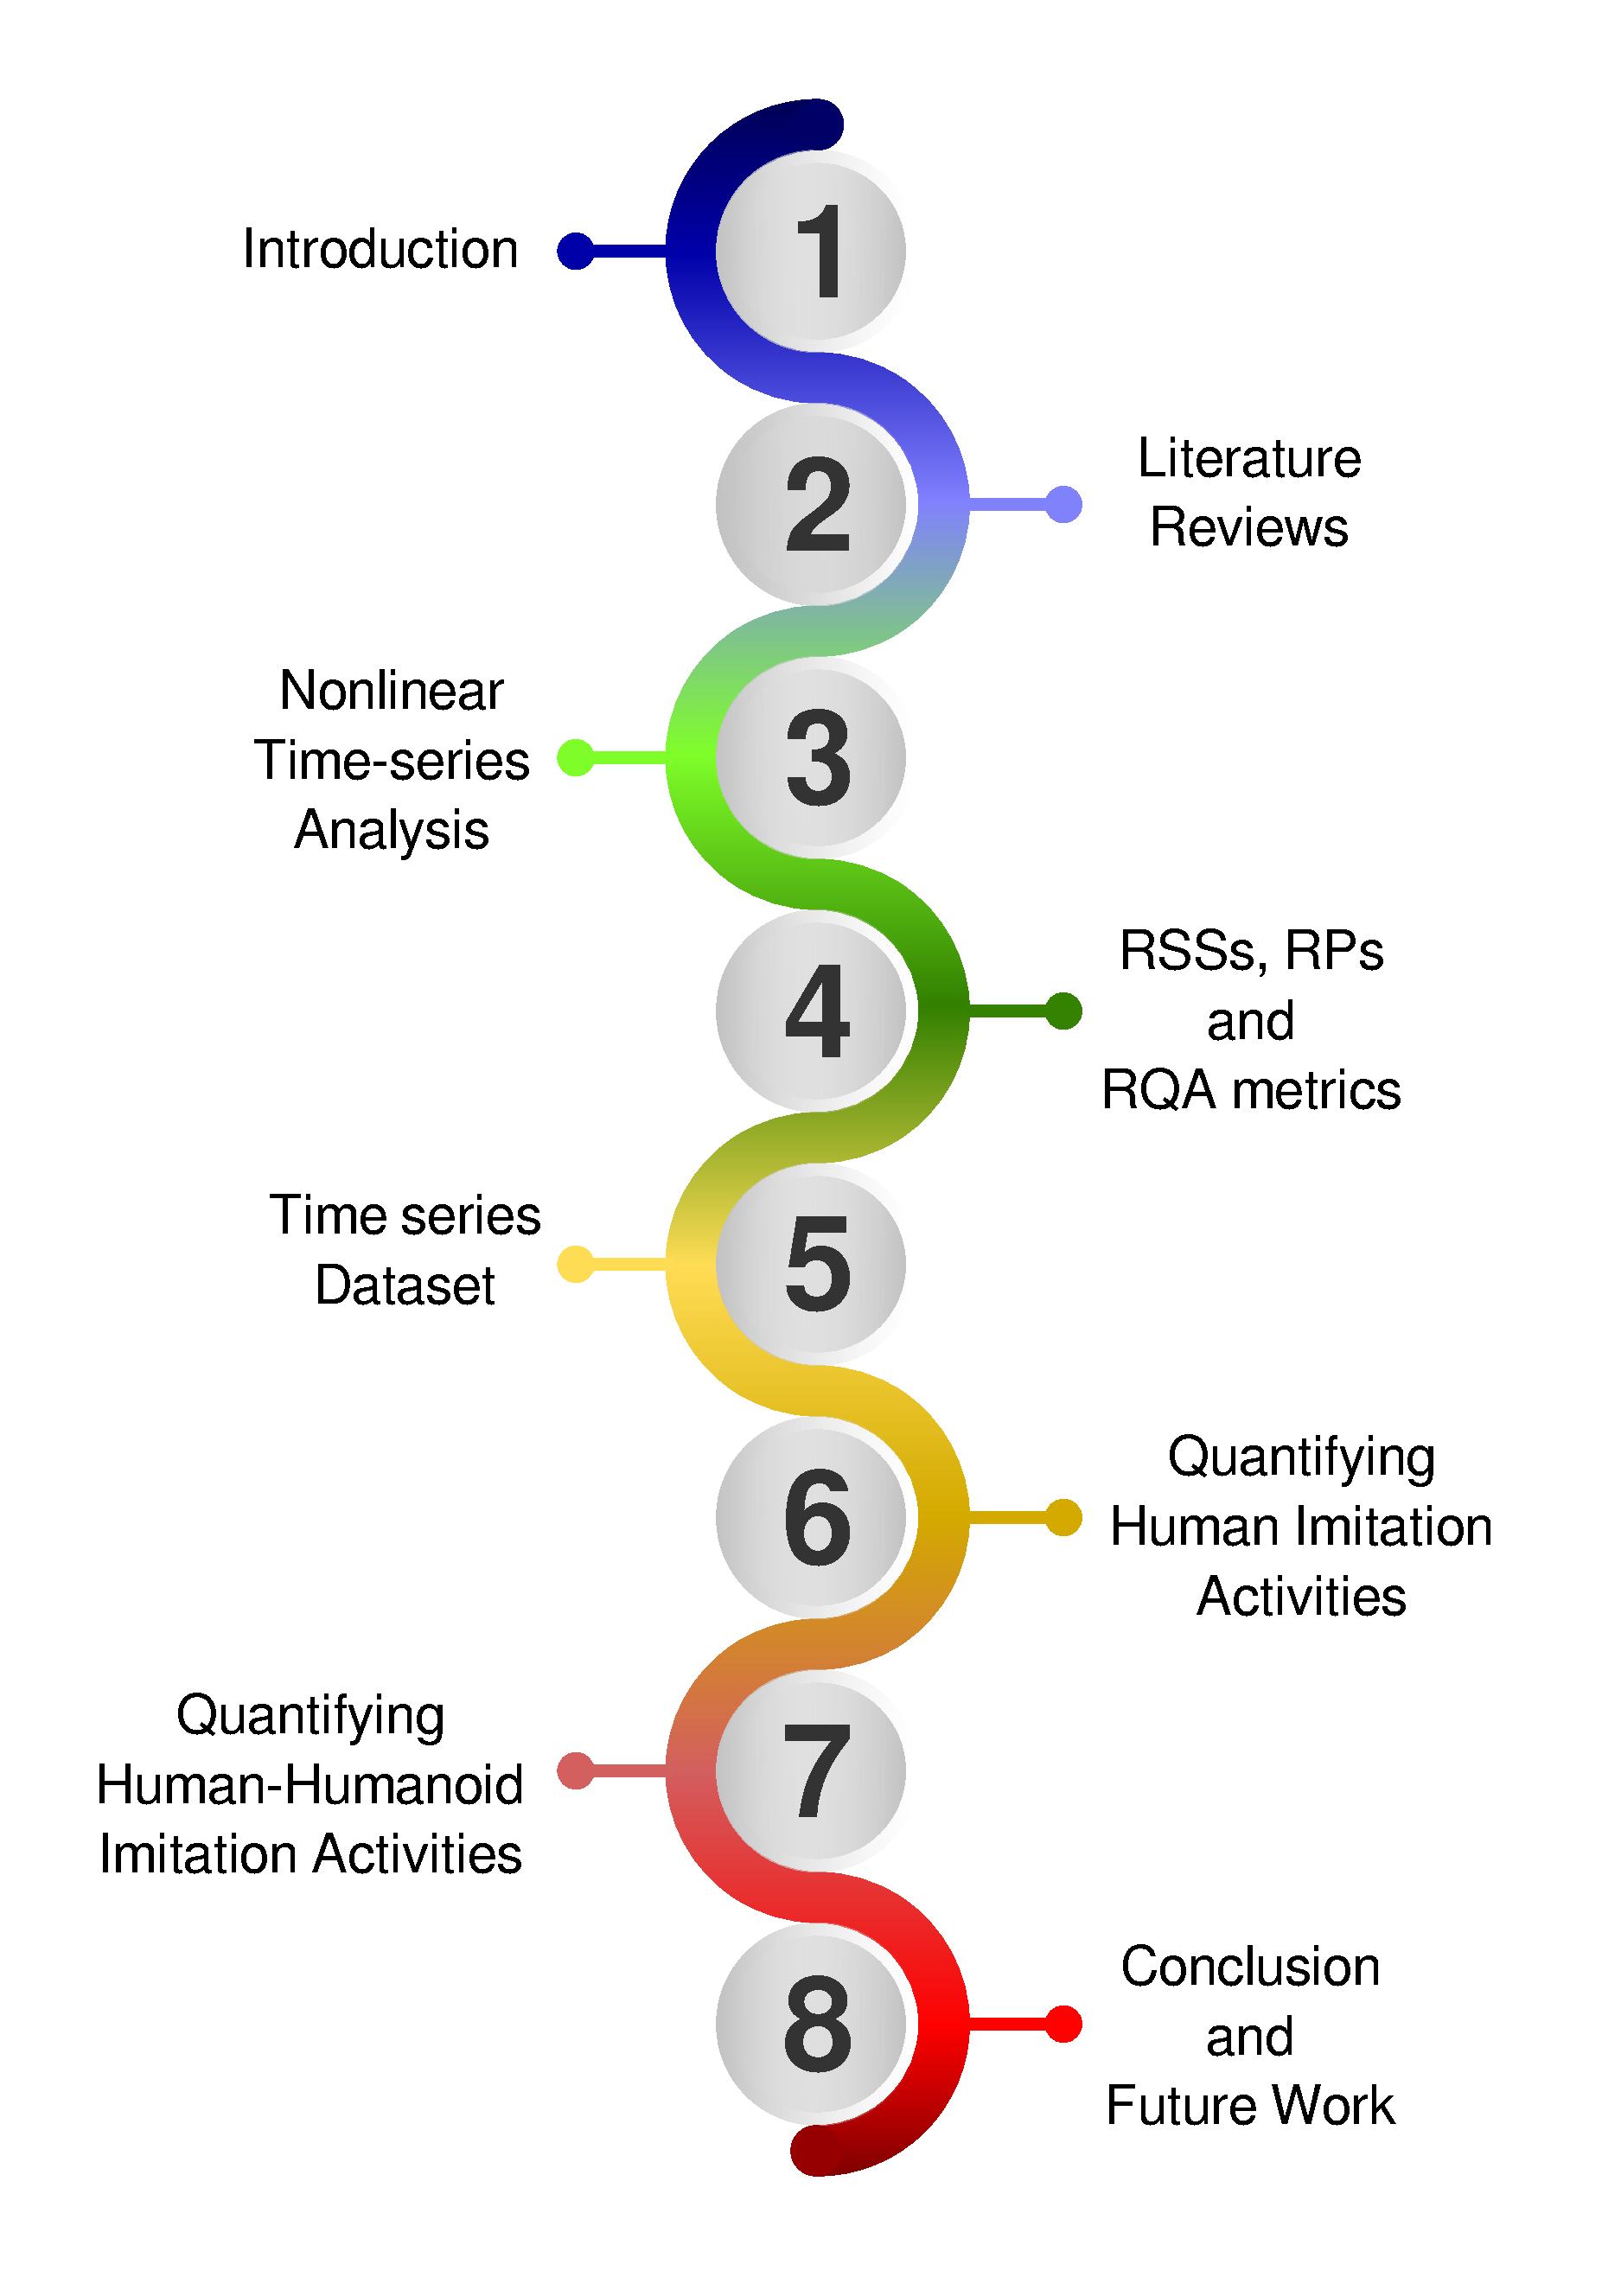
\includegraphics[width=1.0\textwidth]{thesis-structure-v01}
    \caption{
	{\bf Thesis structure.}
	One to eight numbers represent the chapter number.   
	  }
    \label{fig:ts}
\end{figure}
%%---------------------------------(FIGURE)-------------------------------------





\section{Publications}
Partial work of this thesis has been published in the following peer-reviewed conferences.
\begin{itemize}
\item Xochicale M., Baber C., and Oussalah M.,
	Understanding Movement Variability of Simplistic Gestures Using an Inertial Sensor,
	in Proceedings of the 5th ACM International Symposium on Pervasive Displays, 
	Oulu, Finland, June 2016, 
	pages 239--240.

\item Xochicale M., Baber C., and Oussalah M.,
	Analysis of the Movement Variability in Dance Activities Using Wearable Sensors,
	in Wearable Robotics: Challenges and Trends,
	Segovia, Spain, October 2016,
	pages 149--154.

\item Xochicale M., Baber C., and Oussalah M.,
	Towards the Quantification of Human-Robot Imitation Using Wearable Inertial Sensors,
	in Proceedings of the Companion of the 2017 ACM/IEEE International Conference on Human-Robot Interaction,
	Vienna, Austria, March 2017,
	pages 327--328.

\item Xochicale M., and Baber C.,
	Towards the Analysis of Movement Variability in Human-Humanoid Imitation Activities,
	in Proceedings of the 5th International Conference on Human Agent Interaction,
	Bielefeld, Germany, October 2017,
	pages 371--374.
\end{itemize}


 %Introduction
%%*******************************************************************************
%****************************** Second Chapter *********************************
%*******************************************************************************

\chapter{Quantifying Movement Variability}

%% **************************** Define Graphics Path **************************
%\ifpdf
%    \graphicspath{{chapter2/figs/raster/}{chapter2/figs/PDF/}{chapter2/figs/}}
%\else
%    \graphicspath{{chapter2/figs/vector/}{chapter2/figs/}}
%\fi
%


%**************************** %Intro  ***********************************
\section{Introduction}


It has been stated in Chapter 1 that movement variability can be modelled
and quantified using nonlinear tools mainly because the structures of the 
human physiology (lungs, neurons, etc.) suggest that many of their dynamics 
are controlled by nonlinear dynamics \citep{goldberger1990}
and data from human movement is essentially chaotic deterministic, 
meaning that it is neither deterministic nor stochastic 
\citep{hatze1986, preatoni2010, preatoni2013, stergiou2006}. 
Additionally, data from the human body is 
generally noisy, deterministic, stochastic or nonstationary 
\citep{newell1998}.
Therefore, in this chapter fundamentals of time series, nonlinear tools and
nonlinear tools with real-data will be reviewed.


%\cite{stergiou2006}
% mentioned that the reduction or increase of chaotic
%temporal representations is related to a decline of 
%"healthy flexibility associated with behavioral rigidity and inability 
%to adapt to stress placed in the human body." 
%%Before going any further with nonlinear analysis, we have to 
%

\section{Fundamentals of time-series analysis}
Biosignals from living systems can typically be nonstationary, nonlinear, 
deterministic chaotic and noisy \citep{klonowski2007, caballero2014, 
wijnants2009, gomezgarcia2014, stergiou2006, harbourne2009, stergiou2011,
hatze1986, newell1998}. Therefore, it is important to provide fundamental 
definitions of time series which will be used thought the thesis.

\subsection{Linear and nonlinear systems}
Linear systems are proportional or additive. For example, the interaction 
between variables of a linear system are negligible whereas for a nonlinear 
system such interaction of variables can produce emergent properties 
due to the initial conditions of the system \citep{klonowski2007}.

\subsection{Stationary and nonstationary signals}
Stationary signals have the same mean and variance as time progress (e.g. 
a sinusoidal signal), however such stationary signal can also be changeable
(e.g. alternative sinusoidal signal).
In contrast, when statistics of the time series change with time then 
such signal is known as nonstationary signal.
Nonstationary signals are therefore characterised by having transients and 
drifts over time. Examples of nonstationary signals are the time series of 
seasonal trends and changes \citep{kitagawa1984}, Electroencephalography (EEG) 
signals which present different and changeable intensity over time 
\citep{klonowski2007}.

\subsection{Deterministic and stochastic systems}
A deterministic systems means that is predictable. Deterministic systems 
have the characterising to have small number of variables of importance 
in the system. Deterministic systems are modelled with linear ordinary 
differential equations and their initial conditions and constants.
In contrast, stochatic systems are nonpredictable and therefore have 
bigger number of variables of equal importance and stochastic systems are 
modelled with probability theory \citep{klonowski2007}.

\subsection{Deterministic chaotic time series}

Deterministic signals can dramatically change with a slight change 
of initial conditions and then after a long time-scale, the signal can 
appear to be stochastic \citep{amato1992}. Similarly, 
\citealt[p. 11]{klonowski2007} pointed out that "chaotic systems behave 
like they were stochastic but they are also deterministic", meaning that 
chaotic systems are predictable for a short time-scale but nonpredictable 
in a long time-scale because of the initial conditions of the systems. 
Then, \citealt[p. 78]{preatoni2013}, in experiments in sport science, mentioned 
that "variability is likely to have both deterministic and a 
stochastic origin". Therefore, it can be concluded that time series for 
human body movement are neither independent nor stochastic but 
deterministic chaotic \citep{stergiou2006, harbourne2009, stergiou2011}.
%\subsubsection{Lorenz systems. A deterministic chaos system}
%replicate 3.3 of 
%\citep{klonowski2007}


\section{Quantifying Movement Variability with Nonlinear Dynamics}


\subsection{Introduction}
Previous studies have shown that movement variability is not considered 
as a undesired factor that creates errors but a signature for 
assessment of healthiness (associated with unhealthy pathological states) 
or skillfulness (associated with the functionality of movement) 
\citep{stergiou2011}. Fundamentally, movement variability can be either 
quantified based on magnitude of the variability or the dynamics and 
complexity of the variability \citep{caballero2014}. However, finding 
the right tools to quantify movement variability is still an open problem. 

For instance,
%Similarly, 
\cite{preatoni2010, preatoni2013} pointed 
out that conventional statistics (e.g. standard deviation, coefficient 
of variation, intra-class correlation coefficient) only quantify 
the overall variability.
%\cite{preatoni2010, preatoni2013} pointed out that subtle changes in the 
%neuro-muscular-skeletal system are caused by influences of environmental 
%changes, training procedures or latent pathologies. Hence, measuring such 
%variables with conventional statistics (e.g. standard deviation, 
%coefficient of variation, intra-class correlation coefficient) is only 
%for overall variability. 
Also, \cite{stergiou2011} stated that statistical tools 
(e.g. mean, standard deviation and the range) are a measure of centrality,
meaning such metrics are compared around a central point. Similarly, 
\cite{coffey2011} pointed out that the use of means and standard deviations 
led to reduction of data and information is therefore discarded.

%Additionally, \cite[p. 24]{goldberger2002b} 
%stated that "no single statistical measure can be used to assess the complexity of 
%physiologic systems" which is an illustration of the limitations of 
%


Additionally, one can apply frequency-domain tools to quantify movement 
variability.
For example, \cite{hatze1986} proposed a measure of dispersion to 
quantify the deviation of motion from a certain reference using the 
Fourier series. However, deviations of motion are from angular coordinates 
(radians) and linear coordinates (meters) which made them an unacceptable 
fusion of variables. 
\cite{vaillancourt2001} pointed out that it is rare for frequency and 
amplitude to differ in postural tremor of patients with Parkinson's disease
but differences in time-dependent structures are apparent, and associated with 
a change of regularity of postural tremor.
Then, \citep{klonowski2002, klonowski2007, klonowski2009} stated that 
frequency-domain tools require to have stationary data, otherwise using 
other type of data might create misleading results.
%One example is the decompositon of FFT into sine function
%that for instace fail to repsent a 12 hz signal with a modulated amplotude 
%into a two freuqnecy of 11 and 13 hz and the main frequency of 12Hz dissaperis.
%%%%MAKE A STRONGER STATEMENT FOR THE FOLLOWING PARAGRAPH
%In contrast, \cite{preatoni2013} mentioned that Fourier basis approach 
%may be appropriate for periodic signals while wavelet analysis may be for 
%noisy data which contains informative spikes.

%Recently, \cite{preatoni2013} investigated that movement variability is 
%considered as a compensation of noise in the neuro-musculo-skeletal system 
%and the exploration of different strategies of movements to find the most
%appropriate pattern for the actual task. 
%Such compensation of noise and adaptation of movements cannot be
%quantified entirely with the use of conventional approaches for which 
%non only the use of entropy measures (SampEn and ApEn) but 
%Lyapunov exponent \cite{abarbanel1993, smith2010}.
%

Therefore, applying either statistical tools or frequency-domain tools 
to quantify movement variability might create misleading results, 
specially when dealing with signals that are deterministic chaotic 
\citep{amato1992, dingwell2000, dingwell2007, miller2006},
considering  
%With that in mind, \cite{preatoni2010, preatoni2013} stated 
that the subtle changes in the neuro-muscular-skeletal system are caused by 
influences of environmental changes, training procedures or latent 
pathologies \citep{preatoni2010, preatoni2013}
and that movement variability involves evolution of human movement and 
exploratory nature of movement \citep{stergiou2011, caballero2014}. 
Hence, \cite{stergiou2011, preatoni2010, caballero2014} 
highlighted that movement variability can be better described and quantified 
with different nonlinear dynamics tools such as: 
%correlation dimension
largest Lyapunov exponent \citep{bruijn2009, donker2007, kurz2010b, 
yang2011},
fractal analysis \citep{delignleres2003},
entropy rate \citep{cavanaugh2010},
Sample Entropy (SampEn)  \citep{richman2000, donker2007, liao2008, 
stins2009, vaillancourt2004},
Approximate Entropy (ApEn) \citep{pincus1991, kurz2010a, sosnoff2006, 
sosnoff2009, cavanaugh2010},
Fuzzy Entropy (FuzzyEn) \citep{chen2007},
Multiscale Entropy (MSE) \citep{costa2002},
Permutation Entropy (PE) \citep{bandt2002, vakharia2015},
Quadratic Sample Entropy (QSampEn) \citep{lake2011},
Amplitude-aware permutation entropy (AAPE) \citep{azami2016},
Detrended Fluctuation Analysis (DFA) \citep{gates2007, gates2008, 
hausdorff200} and 
Recurrence Quantification Analysis (RQA) \citep{zbilut1992, trulla1996, 
marwan2008}.
%(for applications of the tools, see \cite{caballero2014}).
%\cite{caballero2014} reviewed different entropy measures and its application
%in human movevent variability.
%For example, 
%(Smith,Teulier, Sansom, Stergiou and Ulrich, 2011),
%mental fatigue  (Liu,Zhang and Zheng, 2010),
%or changes in intracranial pressure 
%(Hornero, Aboy, Abásolo, McNames and Goldstein, 2005).
%the problems with ApEn is the dpendency wht tiem series length for which,
%in 2000, Richman and Moorman proposed Sample Entropy which has been applied 
%to quantify postural control  (Menayo, Encarnación, Gea and Marcos, 2014),
%or 
%"to find differences between schizophrenia and depression"
%(Hauge, Berle, Oedegaard, Holsten and Fasmer, 2011).
%Then in 2007, Chen et al. develop Fuzzy Entropy which has less
%depency to tdata lenght and offer more robutnsess to noise.
%FuzzyEn has been used to qunatify muscle fatique 
%(Xie, Guo and Zheng, 2010)
%to qunatify the problems in satanding  balance tasks 
%(Barbado et al.,2012).
%Multiscale Entropy Costa, Goldberger and Peng (2002)
%Permutation Entropy Vakharia et al. (2014),
%Bandt and Pompe (2002).


%RQA is applied for postural fluctations or
%heart rate varialibyt that measure the regularity of time series 
%\cite{caballero2014},



%
%

%\subsection{Measures of Variability}
%%Measuring movement variability represent also a challenge where for instance 
%%traditional approaches in statistics or frequency domain tend to fail when 
%%measuring different types and sources of variability.
%
%\cite{hatze1986} proposed a measure of dispersion to quantify the deviation 
%of motion from a certain reference using the Fourier series. In this approach,
%deviations are from angular coordinates (radians) and linear coordinates 
%(meters) which made them an unacceptable fusion of variables.
%
%Hence, \cite{hatze1986} proposed the use of transentropy as a global quantifier 
%for motion variability which is able to measure dispersion considering that any 
%movement deviation on a body join may be the result of deterministic and 
%stochastic causes.
%Also, \cite{hatze1986} pointed out that transentropy, as a mesuremente of 
%motion variabilty, is fundamental to compute other metrics such as 
%average transentropy, weighted global transentropy or time transentropy.
%%\cite{hatze1986} It is also important to note that experimental work of measuring
%%running cycles, Hatzel1986 can quantify the variability between four
%%cycles of running where the initial cycle has the largest (60m) 
%%then it decreased and stay stable until (1600m) and then again
%%increased at the final phase. 
%
%\cite{vaillancourt2001} pointed out that it is rare for frequency and amplitude 
%to differ in postural tremor of patients with Parkinson's disease
%but differences in time-dependent structures are apparent, and associated with 
%a change of regularity of postural tremor.
%Therefore, \cite{vaillancourt2001} considered appreciate entropy (ApEn) 
%to quantify such regularity in time-dependent structures.
%%Entropy metrics (Approximate Entropy ApEn, Sample Entropy SamEn) quantify the 
%%regularity of time series either for kinematic or kinetic measure and therefore 
%%the increase of regularly means that there is a decrease in the complexity of 
%%the system that produce the time series therefore such decrease in complexity 
%%is associated with pathological conditions \cite{vaillancourt2001}.
%
%
%\cite{preatoni2010} pointed out that subtle changes in the 
%neuro-musculo-skeletal system are caused by influences of environmental 
%changes, training procedures or latent pathologies. Measuring such 
%variables with conventional statistics (e.g. standard deviation, 
%coefficient of variation, intra-class correlation coefficient) is 
%only for overall variability. Therefore, using nonlinear dynamics tools 
%such as sample entropy (SampEn) and approximate entropy (ApEn) can help 
%to analyse the deterministic and stochastic origin of movement variability.
%%using SampEn with original sources of ... and surrogate data where time series maintain 
%%large-scale structures like periodicity, mean, variance and spectrum and 
%%eliminate small-scale structures like chaotic, linear/nonlinear-determinism.
%%It is hence confirmed experimentally that movement variability is not noise
%%but the information concerning with regards to the  nuero-musculo-skeletal system. 
%%That is because SamEn after surrogation had an increase from 16\% to 59\%,
%%suggesting that the time series is not the outcome of a random process \cite{preatoni2010}.
%Recently, \cite{preatoni2013} investigated that movement variability is 
%considered as a compensation of noise in the neuro-musculo-skeletal system 
%and the exploration of different strategies of movements to find the most
%appropriate pattern for the actual task. 
%Such compensation of noise and adaptation of movements cannot be
%quantified entirely with the use of conventional approaches for which 
%non only the use of entropy measures (SampEn and ApEn) but 
%Lyapunov exponent \cite{abarbanel1993, smith2010}.
%%reviewed methods of nonlinear dynamics such as
%%entropy measures as one of the alternative tools compared to the traditional
%%ones to investigate the nature of movement variability in elite athletes.
%%Research on quantifying pathologies with nonlinear dynamics has been done,
%%however, very little work were reported concerning movement variability in sport 
%%science due to limited availability of data.
%
%
%

%\subsection{What to measure in movement variability (MV)?, 
%how to measure MV? and which tools are appropriate to measure MV?}

Having got many nonlinear tools to measure movement variability (MV) 
made \citealt[p. 67]{caballero2014} to raise the following question: 
"Is there a best tool to measure variability?" which leads us to 
formulate a further set of questions for this thesis on 
what to measure in MV?, how to measure MV? 
and which tools are appropriate to measure MV?

\subsection{What to measure in MV?} \label{what_to_measure_with_MV}
\cite{vaillancourt2002, vaillancourt2003} stated that there is no universal 
increase or decrease in complexity for MV as a function of age or disease 
but a dependency with the task dynamics. For example, in a constant-force 
task (where the task dynamics is of low dimension), generally older adults 
present less complexity due their inability to introduce additional degrees 
of freedom in the neuromuscular system. However, there is an increase of 
complexity in older adults or unhealthy adults when the task dynamic is 
oscillatory because these type of adults have more difficulty to reduce 
the dimension output to a lower dimension which are the intrinsic dynamics 
of their resting state.

In contrast, inspired by \cite{tononi1998} who modelled complexity 
in neural networks considering complexity versus regularity variables,
%where complex systems are neither completely random nor completely regular,
%TODO: extend the conclusions made by tononi1998
\cite{stergiou2006} proposed a model of complexity versus predictability 
variables for optimal human movement variability.
The model of \cite{stergiou2006} stated that higher complex movements are 
associated with rich behaviour of movements while lower complex movements 
are associated with poor behaviours of movements being too rigid or too 
unstable. Hence, higher complex movements are therefore characterised by 
chaotic systems, while lesser complexity of movements are characterised either 
as noisy systems or periodic systems (having either low amounts of 
predictability or hight amounts of predictability) \citep{stergiou2006}.
%FUSE PREVIOUS PARAGRAPH WITH THE FOLLOWING
%Similarly, in the neurobiology field, find the problem of assosiating random 
%molecules of gas or regular organisation of molecues of cristals with low complexity 
%but at the same time associated them with a level or regularity,
%for which \cite{tononi1996, tononi1998} proposed a statistical mesuare based on the deviation 
%form the independence (mutual information) to to capture the regularities  amongt subtes of systems.
%Hence, \cite{stergiou2006} proposed a model that relates 
%health and motor learning based on the work of \cite{tononi1996, tononi1998}.
%In the model for 
%\cite{stergiou2006} stated that greater amounts of complexity are related to
%rich behavioral states which are therefore associated with chaotic structures.
%In constrast, lesser amounts of complexity are associated with both 
%random or periodic which are also related to the amount 
%of predictability. Therefore, random and noisy systems are associated 
%with low predictability, while periodic, repeatable and rigid behaviors
%are associated with  high amounts of predictability.



%\subsection{How and with what to measure?}
%\subsection{How to measure MV? and which tools are appropriate to measure MV?}
\subsection{Which nonlinear tools are appropriate to measure MV?} 
\label{which_NT_are_appropriate_to_measure_MV}


Considering the model of \cite{stergiou2006} for movement variability,
where complexity and predictability variables of a system can 
characterise and quantify movement variability, it is important to 
find, to understand and to apply the right tools that measure such variables.

%With that in mind, \cite[p. 67]{caballero2014} raised an important question 
%regarding the quantification of movement variability: "Is there a best tool 
%to measure variability?". To the best of our knowledge, the answer is no. 
%However, let us dig in further into the literature and provide 
%state-of-the-art references that support our answer.


Originally, \cite{pincus1991, pincus1995} proposed Approximate Entropy (ApEn) 
to quantify regularity of time series.
Then, \cite{richman2000} found that the algorithm of ApEn match itself 
to avoid the occurrence of ln(0) which made ApEn dependant on the available 
data for which Sample Entropy (SampEn) were proposed as an algorithm that 
does not consider self-matching. 
Hence, SampEn values are independent of the length of time series and its 
algorithm is simpler than ApEn.
Then, instead of using single statistics, \cite{costa2002} proposed 
Multiscale Entropy (MSE) algorithm which computes SampEn of consecutive 
coarse-grained time series of the original time series defined by the 
scale factor, $\tau$.
%where the length of each time series is divided 
With MSE algorithm, \citep{costa2002} noted that 
pathology dynamics for time series of heartbeat intervals 
%e.g. "increase of regularity and decrease of variability or
%increase of variability due to loss of correlation properties", 
are associated with reduction of complexity.
Therefore, \citealt[p. 3]{costa2002} concluded that physiologic complexity 
is associated to the adaptive capacity of the organism,  
diseases states and aging which "may be defined by a sustained 
 breakdown of long-term correlations and loss of information".
%Although, for large scales healthy vs pathology signals can be
%distinguishable, the pathological signals overall and become 
%indistinguishable.
Essentially, entropy measures (AppEn and SampEn), 
quantify regularity and complexity of time series \citep{preatoni2013}.
%For instance,  Approximate Entropy (AppEn) values are in a range 
%between 0 and 2.
%AppEn values closer to 0 are associated with time series of greater 
%periodicity and regularity (e.g. sine wave) and 
%AppEn values near to 2 are associated with irregularity 
%(e.g. random time series) \citep{miller2006}.
%However, \cite{caballero2014} stated that is not clear how 
%\cite{goldberger2002b} and \cite{vaillancourt2002} applied entropy metrics 
%to analyse movement complexity.
However, \cite{goldberger1996} mentioned that the increase of irregularity 
in time series is not a synonymous of increase of physiologic complexity.
Similarly, an increase of ApEn or SampEn, "implying increase of irregularity 
and decrease in predictability" \cite[p. 25]{goldberger2002b}, is not 
synonymous of an increase of dynamical complexity when analysing physiology 
signals \citep{costa2002}.
Hence, \cite{goldberger2002b} demonstrated that ApEn as a regularity 
statistic is not a direct index of physiologic complexity where, for example, 
a randomised time series of an healthy heartbeat with multi-scale and 
complex patterns of variability show a higher value of ApEn being that 
the time series is less complex. Therefore, \citealt[p. 24]{goldberger2002b} 
concluded that the loss of physiologic complexity can be 
"better assessed using other measures which can detect and quantify the 
presence of long-range correlations in nonstatiorany series."
Hence, \cite{goldberger2002b, vaillancourt2002, costa2002} concluded that
ApEn and SampEn do not necessary show the right representation of what 
they are intent to measure. 
%Additionally, \cite[p. 24]{goldberger2002b} 
%stated that "no single statistical measure can be used to assess the complexity of 
%physiologic systems" which is an illustration of the limitations of 
%using single statiscts \citep{caballero2014}.

%However,that Fractals are irregular but 
%"not all irregular structures or erratic time series are fractal \cite{goldberger1996}.
%Hence, fractal features can also be used to assess complexity 
%of movement variability \cite{holden2005, vanorden2003}



Therefore, considering the previous cons of ApEn, SampEn and MSE, Detrended 
Fluctuation Analysis (DFA), which is based on analysing fractal features, 
can quantify long-term correlations of time series \citep{peng1995}.
%Considering that ApEn is a regularity statistic, 
%the increase of ApEn when destroying fractal and nonlinear properties 
%of heartbeat time series by a randomised prodecure 
%might be related to a breakdown in long-range correlations
%"or due to subtle perturbations in nonlinear control".
%of long auto-correlation for nonstationary time series 
%and "avoid spurious detection of apparent long-range correlations
%that are an artifac of nonstationary time series"
DFA is calculated as the root mean square fluctuation of an integrated 
and detrended time series and it is represented by a scaling exponent, 
$\alpha$, which is an indicator for roughness of time series,
e.g. "the larger the value of $\alpha$, the smoother the time series 
\citep[p. 83]{peng1995}.
However, only using  DFA can result in a false conclusion for long term 
correlations in the time series \cite[p. 5001]{rangarajan2000}, therefore 
DFA "can falsely classify certain type of time series as fractals" 
\cite[p. 80]{wijnants2009}.
With that in mind, \cite{wijnants2009} proposed the use of RQA as a 
technique that does not present any constraints with regards to length size,
stationary or statistical distribution of the time series.
Nonetheless, \cite{wijnants2009} highlighted that  SampEn index is calculated 
over the sequential values of the time series, whereas Shannon entropy in 
RQA which is computed over the distribution of deterministic lines in 
the Recurrence Plots (RP) \citep{marwan2008, trulla1996, zbilut1992}.
Similarly, \cite{rhea2011} highlighted that algorithms to compute entropy 
measures are different since ApEn and SampEn are approximations of the 
Kolmogorov-Sinai Entropy computing the likelihood that a template pattern 
repeats in the time series while RQAEn is derived from Shannon entropy 
and is computing number of line segments of varying length in the RP.
Even though with those difference in the algorithms, smaller values of 
recurrence percentage of the RQA shown the increase of practice of movement
dynamics, concluding that such recurrence percentage is indicator of 
increase of system stability \citep{wijnants2009}.



%"movement trajectories evolve in a more confined region
%through their phase-space \cite[p. 89]{wijnants2009}.
%", also SampEn drops as practice is increasing
%which indicate lower-dimensional organisation of coordinate structures 
%\cite[p. 89]{wijnants2009}.




%
%\cite{higuchi1988} introduced a method to 
%compute the fractal dimensionality for non-periodic and irregular time series
%and test its robustness against other methods.
%
%Recently, \cite{klonowski2007} 
%using higuchi method the complexity of a time series can be used in different
%scenarios of depth of anesthesia, bright light therapy, postural analysis, etc.
%
%Also, another of the advantes of Higuchi's method pointed out by 
%\cite{klonowski2002, klonowski2007, klonowski2009}
%is that fractal can be computed only in time domain wotuhgotuih
%comptuing a satate spacewhich si offent computataiton
%and requries expreitse.
%Huguchi method is robust to noise signasl \cite{klonowski2002} 
%
%However, \cite{klonowski2002, klonowski2007, klonowski2009}
%it is highlighthed that fractal dimension computed by higuchi's mehtod 
%is different than the fractal dimension computed in teh state space representtation.
%%MORE DETAILS!


Another tool to measure variability is the largest Lyapunov exponent (LyE) 
which "quantify the exponential separation of nearby trajectories
in the reconstructed state space of a time series" \citep[p. ??]{stergiou2004}.
%\cite{caballero2014} stated that local dynamic stability is defined
%as a metric of sensitivity to small perturpations with are generally 
%measured with LyE.
For instance, "LyE from a stable system with little to no divergence will 
be zero (e.g. sine wave)" and "LyE for an unstable system that has highest 
amount of divergence will be positive and relative hight in value
(e.g. 0.469 for random noise)" and for chaotic systems like the Lorenz system,
LyE is in between the two of the previous extremes (LyE$\approx0.1$) 
\cite[p. 2874]{miller2006}. However,  LyE requires to be validated using 
surrogation \citep{dingwell2000, miller2006}.
%because of the time series is deterministic chaotic.
%We refer the reader to \cite{wolf1985} for more details about LyE 
%and to \cite{theiler1992} for surrogation.

%\subsection{Is there a best tools to measure variability?}


Measuring human movement variability requires a combination of the 
pros and cons of many of the previous tools that analysis either 
(i) the dynamic complexity or (ii) the degree of regularly, stability or 
predicability in a system \citep{goldberger2002b, harbourne2009, stergiou2011}.
For instance, \cite{rangarajan2000} stated the use of both spectral analysis 
and random walk analysis, the base of DFA, is a better approach than only 
using one tool which can lead to false conclusion for long term correlations
in the time series.
Similarly, \cite{wijnants2009} selected different tools (spectral analysis, 
standard dispersion analysis, DFA, RQA and SampEn) to quantify movement 
variability that can complement the strengths of some of them and also 
compensate the weakness of others. Recently, \cite{caballero2014} proposed 
the unification of different tools to address every aspect of the dynamics 
of a systems and the characterisation of the variability. 

Although, there is no best tool to measure movement variability and an 
unification of tools to quantify human movement variability is still an 
open question, finding the right tool to measure movement variability 
for an specific problem, and knowing its strengths and weakness of such 
tool is one of the research questions for this thesis. 
%Therefore, the contribution to knowledge of this thesis is about the 
%reliability of the  Recurrence Quantification Analysis (RQA) metrics using 
%different conditions of the time series.


\section{Nonlinear analyses with real-world data} \label{nonlieaRealdata} 
Recently, \cite{huffaker2017} only highlighted that one of the caveats 
when applying nonlinear time series analysis tools is its unreliability 
when the estimated metrics come from real-world data which is generally 
short, noisy and nonstationary. Similarly, \cite{preatoni2013} mentioned 
the limitations of the use of nonlinear analyses in sport activities 
where data required to be large (e.g. number of trials, duration of the 
experiment and sampling frequency). Whereas \cite{caballero2014}, 
providing further a investigation, stated the weaknesses of different 
nonlinear tools regarding the characteristics of the time series such 
as nonstationarity, length data size, noisy, sampling rate.
%which will be explained below.
However, in the work of \cite{huffaker2017}, \cite{preatoni2013} and
\cite{caballero2014} no further exploration of the metrics with 
real-world data is presented.



%%INCORPORATE
%The lower dimension signals from biological signals are generally time series 
%of one-dimension in $\mathbb{R}$ which commonly have 
%high nonlinearity, complexity, and non-stationarity \citep{gomezgarcia2014}.
%


\subsection{Nonsationarity}
Nonstationarity of time series signals might create
spurious increase or decrease in the metrics of nonlinear tools. 
For instance, \cite{costa2007} noted that nonsatiornary in the signals might 
alter the increase of irregularity of signals for the shortest scales when 
applying MSE.  Also, \cite{dingwell2000} reported nonstationary in time series 
when using LyE, which required to be validated using surrogation 
to ensure the robustness of the metric. 
Hence, \cite{caballero2014} reported three options when dealing with 
nonstaionary data: (i) remove nonsatiornary data, (ii) use empirical mode 
decomposition (EMD), and (iii) apply nonlinear tools, such as DFT and RQA, 
which are less sensitive to nonstationary data.

To remove nonstationary data, for example, \cite{carroll1993} suggested 
to remove the trends or to eliminate the first 20 seconds of samples to 
ignore the trend of time series. %of postural sway.
Hence, \cite{vandieen2010}, in experiments with center of pressure movements 
in seated balancing, discarded the first 5 seconds of the time series 
in the start of the measurement to avoid nonstationary of the data.

Also, nonstatioinary time series can be treated with Empirical Mode 
Decomposition (EMD) method which decompose nonlinear, nonstatioanry signals 
into their intrinsic frequency components \citep{huang1998, wu-huang2004, 
wu-huang2009}. Hence, \cite{flandrin2004, costa2007} tested that EMD is a 
robust method for detrending and denoising time series and highlighted that 
 EMD does not require selection of input parameters. However, the reliability 
of EMD methods is still an open problem, for instance, an extension of EMD 
called Multivariate Empirical Mode Decomposition (MEMD) has been proposed 
to analyse multiple time series \citep{rehman2010, mandic2013}.
%and many applications have been presented using EMD 
See \citep{wu-hu2006, costa2007, daubechies2011, bonnet2014, mert2018}
for applications of EMD.

%\cite{wu-hu2006} EMD in cariorespiratory sysncronisation
%\cite{costa2007} use EMD to detrend data of postural complexity in the elderly 
%\cite{daubechies2011} proposed a different method with combine wavelet analysis and reallocation method to perform EMD
%\cite{bonnet2014} EMD for integreation of Human Walking 

Finally, one can use of nonlinear tools that are unaffected by nonsttarionary 
of time series such as Detrended Fluctuation Analys (DFA) \citep{hausdorff1995}
%, because removes local trends, \cite{hausdorff1995} %\cite{chen2002}
and Recurrence Quantification Analysis (RQA) \citep{zbilut1992, trulla1996, 
marwan2008}. 
%RQA metrics suffer from senstivitiy to the embedding parameters and 
%threshodl recurrence to which can also create unrealiable reustls.
However, \cite{bryce2012} reported negatives of DFA such as the introduction
of uncontrolled bias, computational expensiveness and mainly highlighting 
that DFA cannot provide a generic protection against the nonstationarities 
of the signals.





%Derivative
%differencing is a technique to remove trends [chatfield1989]
%"the measured physical varialbel is a derivative of
%another fundamental variable"
%\cite{rangarajan2000}



%
%\subsection{Nonlinear tools for nonstationary timeseries}
%Biosignals are tipically nonstationary \cite{klonowski2007, caballero2014, wijnants2009}.
%




\subsection{Data length}
Many of the nonlinear tools are sensitive to time series length 
\citep{caballero2014}.
For example, given that Multiscale Entropy (MSE) is considered as 
statistical measure, the data lengths are recommended to be larger to ensure 
enough samples for the analysis \citep{costa2007}. 
Also, LyE \citep{wolf1985} and  DFA \citep{peng1995} metrics are sensitive 
to data length, while SampEn \citep{rhea2011} and FuzzyEn 
\citep{richman2000, chen2007} are less sensitive the time series length.
However, the metrics of RQA \citep{webber1994, riley1999, wijnants2009}
and PE \citep{zunino2009} are less sensitive to data length.


\subsection{Sampling rate}
One solution when dealing with data length problems is the increase 
or decrease of sampling rate \citep{caballero2014}.
However, \citealt[p. 267]{duarte2008} stated "the increase of sampling rate 
frequency would only increase artificially the data points without 
adding information" which therefore is raise the problem of 
oversamping signals. 
%However no quantification were made with relationship with nonlinear tools. 
Then, \cite{rhea2011} investigated the influence of sampling rate in 
three entropy measures (ApEn, SampEn and RQAEn) concluding that
Ap and RQAEn were robust across to the increase of sampling frequency,
while SampEn presented significant difference across all sampling 
frequencies. \cite{rhea2011} noted that SampEn is more sensitive to 
coliniarities than Ap and RQAEn at higher frequencies which lead to a 
decrease of SampEn. Hence, \cite{rhea2011} concluded that because signals at 
higher frequencies appear to be more regular due to the increase of data, 
therefore producing erroneous entropy results.
%\cite{rhea2011} highlighted the algorithms to compute entropy measures
%are different since ApEn and SampEn are approximations
%of the Kolmogorov-Sinai Entropy 
%computing the likelihood that a template patter repeats in the time series
%while RQAEn is derived from Shannon entropy and is computing
%number of line segments of varying length in the RP.
%
%recommended to increase the collection time than 
%the increase of sampling frequency to obtain large data points,
%since oversampling 
%suggesting that SampEn is more robuts for shorter time series
%when colinarieties are not an issue.
Then, \cite{caballero2013} showed the robustness of SampEn and DFA tools
when using different sampling rate frequencies, stating that frequencies 
near the dynamics of the activity create a more reliable analysis of the 
dynamics using DFA values and tested the statement of \cite{duarte2008} 
that increasing the sampling rate do not increase the gain of information.
\cite{caballero2013} also stated that the decrease of sampling 
rate frequency is recommended because it presents less consumption 
of computational power.






\subsection{Noise}
Another point to consider is the noise of the signals
and how such noise affects nonlinear tools metrics \citep{caballero2014}.
For instance, \cite{rosenstein1993} tested the robustness of LyE against 
three levels of noise (lowest, moderate and highest) noting the unreliability 
of LyE exponents in hight-noise environments.
However, such case of unreliability of the LyE is unreal as the reported 
values of signal-to-noise ratios are substantially slower than the used at 
the experiments of \cite{rosenstein1993}.
Another examples is the work of \cite{chen2009} who compared the 
robustness FuzzEn, ApEn and SampEn metrics against different levels of noise, 
concluding that for a large value of the parameter $r$ of ApEn and SampEn, 
these two metrics can work fine with highest level of noise, however
when noise increase, ApEn and SampEn fail to distinguish time series with 
different level of noise, whereas FuzzEn probe to be robust to such highest 
levels of noise.
Also, \cite{bandt2002} by proposing the Permutation Entropy metric (PeEn)
showed the robustness of PeEn against observational noise and dynamical noise.


Regardless of the source of noise which can be either mechanical 
(due to recording equipment) or physiological (due to different neural noise), 
\cite{rhea2011} highlighted the importance of the effects of noise in three 
entropy measures (ApEn, SampEn and RQAEn) which resulted in different results.
For instance, values for AnEn and SampEn tended to increase as noise was 
added to the signals, while RQAEn  showed an inverse effect, e.g. RQAEn 
values decreased as noise in the signal was increased.
Similar results for synthetic data were also reported by \cite{pellecchia2005} 
where RQAEn values decreased from ($RQAEn \approx 5$) for Lorenz system to a 
($RQAEn \approx 2$) for a periodic signal with a further decrease 
($RQAEn \approx 0.3$) for a sinusoid signal with superimposed noise. 
Therefore, RQA can also be affected by noise \citep{rhea2011}.
However, the effects with regard to noise and also nonstarionarity
can be mitigated with the selection of the right parameters to perform RQA,
particularly, using embedding dimension from 10 to 20 for biological systems 
\citep{webber2005}.

Another solution in order to deal with noisy time series is the use of 
tradition filtering methods, however the attenuation of all frequencies 
of the signal along the with the noise, given a cutoff frequency, can cut 
out information that might be useful for nonlinear time-series. 
Another option is apply DFA, which additionally to the remove of local 
trends, it also reduces the noise of the signal \citep{hausdorff1995}.
Alternatively, filtering strategies for nonlinear time-series data can 
be applied which tailor in a more effective way the properties of 
nonlinear dynamics (see \citealt*{bradley2015} and references therein).


%\cite{preaotin2013}
% smoothging techinques
%if the time series are smooth and non-periodic, 
%then B-splitnes may be approapriate \cite{coffey2011}.
%if the data is noisy with informative spikes then avoiding severe smoothign 
%is necessary for which wavelet analysis may be appropriate.
%
%\cite{cencini2000}



%
 %Quantifying Movement Variability
%%*******************************************************************************
%****************************** Chapter Three **********************************
%*******************************************************************************
\chapter{Nonlinear Analysis} \label{chapter3}

%****************************** Define Graphics Path ***************************
%\ifpdf
%    \graphicspath{{chapter4/figs/raster/}{chapter4/figs/PDF/}{chapter4/figs/}}
%\else
%    \graphicspath{{chapter4/figs/vector/}{chapter4/figs/}}
%\fi
%
\graphicspath{{figs/chapter3/PDF/}}

\section{Introduction}
Nonlinear analysis investigate the dynamics of observed time-ordered data.
Methods of nonlinear analysis, for this thesis, entail determination 
of embedding parameters, state space reconstruction, uniform time-delay
embedding, recurrence plots and recurrence quantification analysis. 

The method of state space reconstruction was originally proposed by 
\cite{packard1980} and formalised by \cite{takens1981}. Since then, various 
investigations and disciplines relative to nonlinear time series analysis 
have benefited from it \citep{aguirre2009, stergiou2011, frank2010, sama2013}.
The method of reconstructed state space (RSS) is based on uniform time-delay 
embedding (UTDE) which is a simple matrix implementation considering the 
embedding 
parameters ($m$ and $\tau$), therefore, matrix represents the reconstruction
of an unknown $d-$dimensional manifold $M$ from a scalar 
time series (e.g. one-dimensional time series in $\mathbb{R}$).
A manifold, in this context, is a multidimensional curved surface within a 
space (e.g. a saddle) \citep{guastello-gregson2011}.
Henceforth, the method of state space reconstruction using a scalar time series 
can preserve dynamic invariants such as correlation dimension, 
fractal dimension, Lyaponov exponents or Kolmogorov-Sinai entropy 
\citep{bradley2015, Quintana-Duque2012, 
Quintana-Duque2013, Quintana-Duque2016, krakovska2015}.
However, 
there are still many challenging research questions to be answered  
with regards to the selection of appropriate embedding parameters 
that preserver the dynamics of a system 
for the computation of methods nonlinear analysis such as RSS, RPs and RQAs.
With that in mind, in the following sections, I describe in more 
detail the state space reconstruction theorem (RSSs), 
uniform time-delay embedding theorem (UTDE), 
methods to compute embedding parameters: 
false nearest neighbours (FNN)
and average mutual information (AMI).
I also introduce fundamentals to Recurrence plots(RPs) and 
Recurrence quantification analysis (RQA).

\section{State Space Reconstruction Theorem} \label{sec:rss}
Following the notation employed in \cite{casdagli1991, garland2016, 
gibson1992, uzal2011, uzal2010, takens1981}, the method of state space 
reconstruction is defined by:
%%********************************[EQUATION]************************************
\begin{equation}\label{eq:ssr}
  s(t)=f^t [s(0)],
\end{equation}
%%********************************[EQUATION]************************************
where $s$, $s: A \rightarrow M$ given that $A \subseteq \mathbb{R}$ and $M 
\subseteq \mathbb{R}^d$, represents a trajectory which evolves in an 
unknown $d-$dimensional manifold $M$, $f: M \rightarrow M$ is an evolution 
function and $f^t$, with time evolution $t \in \mathbb{N}$, is the $t$-th 
iteration of $f$ that corresponds to an initial position $s(0) \in M $ 
\citep{takens1981}.
Then, a point of a scalar time series $x(t)$ in $\mathbb{R}$, can be obtained 
with
%%********************************[EQUATION]************************************
\begin{equation}\label{eq:measurement}
	x(t)=h[s(t)],
\end{equation}
%%********************************[EQUATION]************************************
where $h$ is a function, $h: M \rightarrow \mathbb{R}$, defined on the 
trajectory $s(t)$.

Reconstructed state space can then be described as an $n-$dimensional state 
space defined by $y(t)=\Psi[\boldsymbol{X}(t)]$ where 
$\boldsymbol{X}(t) = \{ x(t), x(t-\tau) , ...,x(t - (m-1)\tau  ) \}$ is the 
uniform time-delay embedding with a dimension embedding $m$ and delay 
embedding $\tau$ and $ \Psi: \mathbb{R}^m \rightarrow \mathbb{R}^n$ is a 
further transformation of dimensionality (e.g. Principal Component Analysis, 
Singular Value Decomposition, etc) being $n \leq m$. With that in mind, 
uniform time-delay embedding, $\boldsymbol{X}(t)$, defines a map 
$\Phi: M \rightarrow \mathbb{R}^m$ such that $\boldsymbol{X}(t) = \Phi(s(t))$,
where $\Phi$ is a diffeomorphic map \citep{takens1981} whenever $\tau > 0$ 
and $m > 2d_{box}$ and $d_{box}$ is the box-counting dimension of 
$M$ \citep{garland2016}.
Then, if $\Phi$ is an embedding of an attractor (i.e. evolving 
trajectories) in the reconstructed state space, a composition of functions 
represented with $F^t$ is induced on the reconstructed state space:
%********************************[EQUATION]************************************
\begin{equation}\label{eq:st}
  \boldsymbol{X}(t)=F^t [\boldsymbol{X}(0)] = \Phi \circ f^t \circ \Phi ^{-1}[\boldsymbol{X}(0)].
\end{equation}
%%********************************[EQUATION]************************************
Hence, an embedding is defined as "a smooth one-to-one coordinate 
transformation with a smooth inverse" \citep[p. 54]{casdagli1991}. 
Figure~\ref{fig:ssr} illustrates the state space reconstruction.
%---------------------------------(FIGURE)-------------------------------------
\begin{figure}
  \centering
    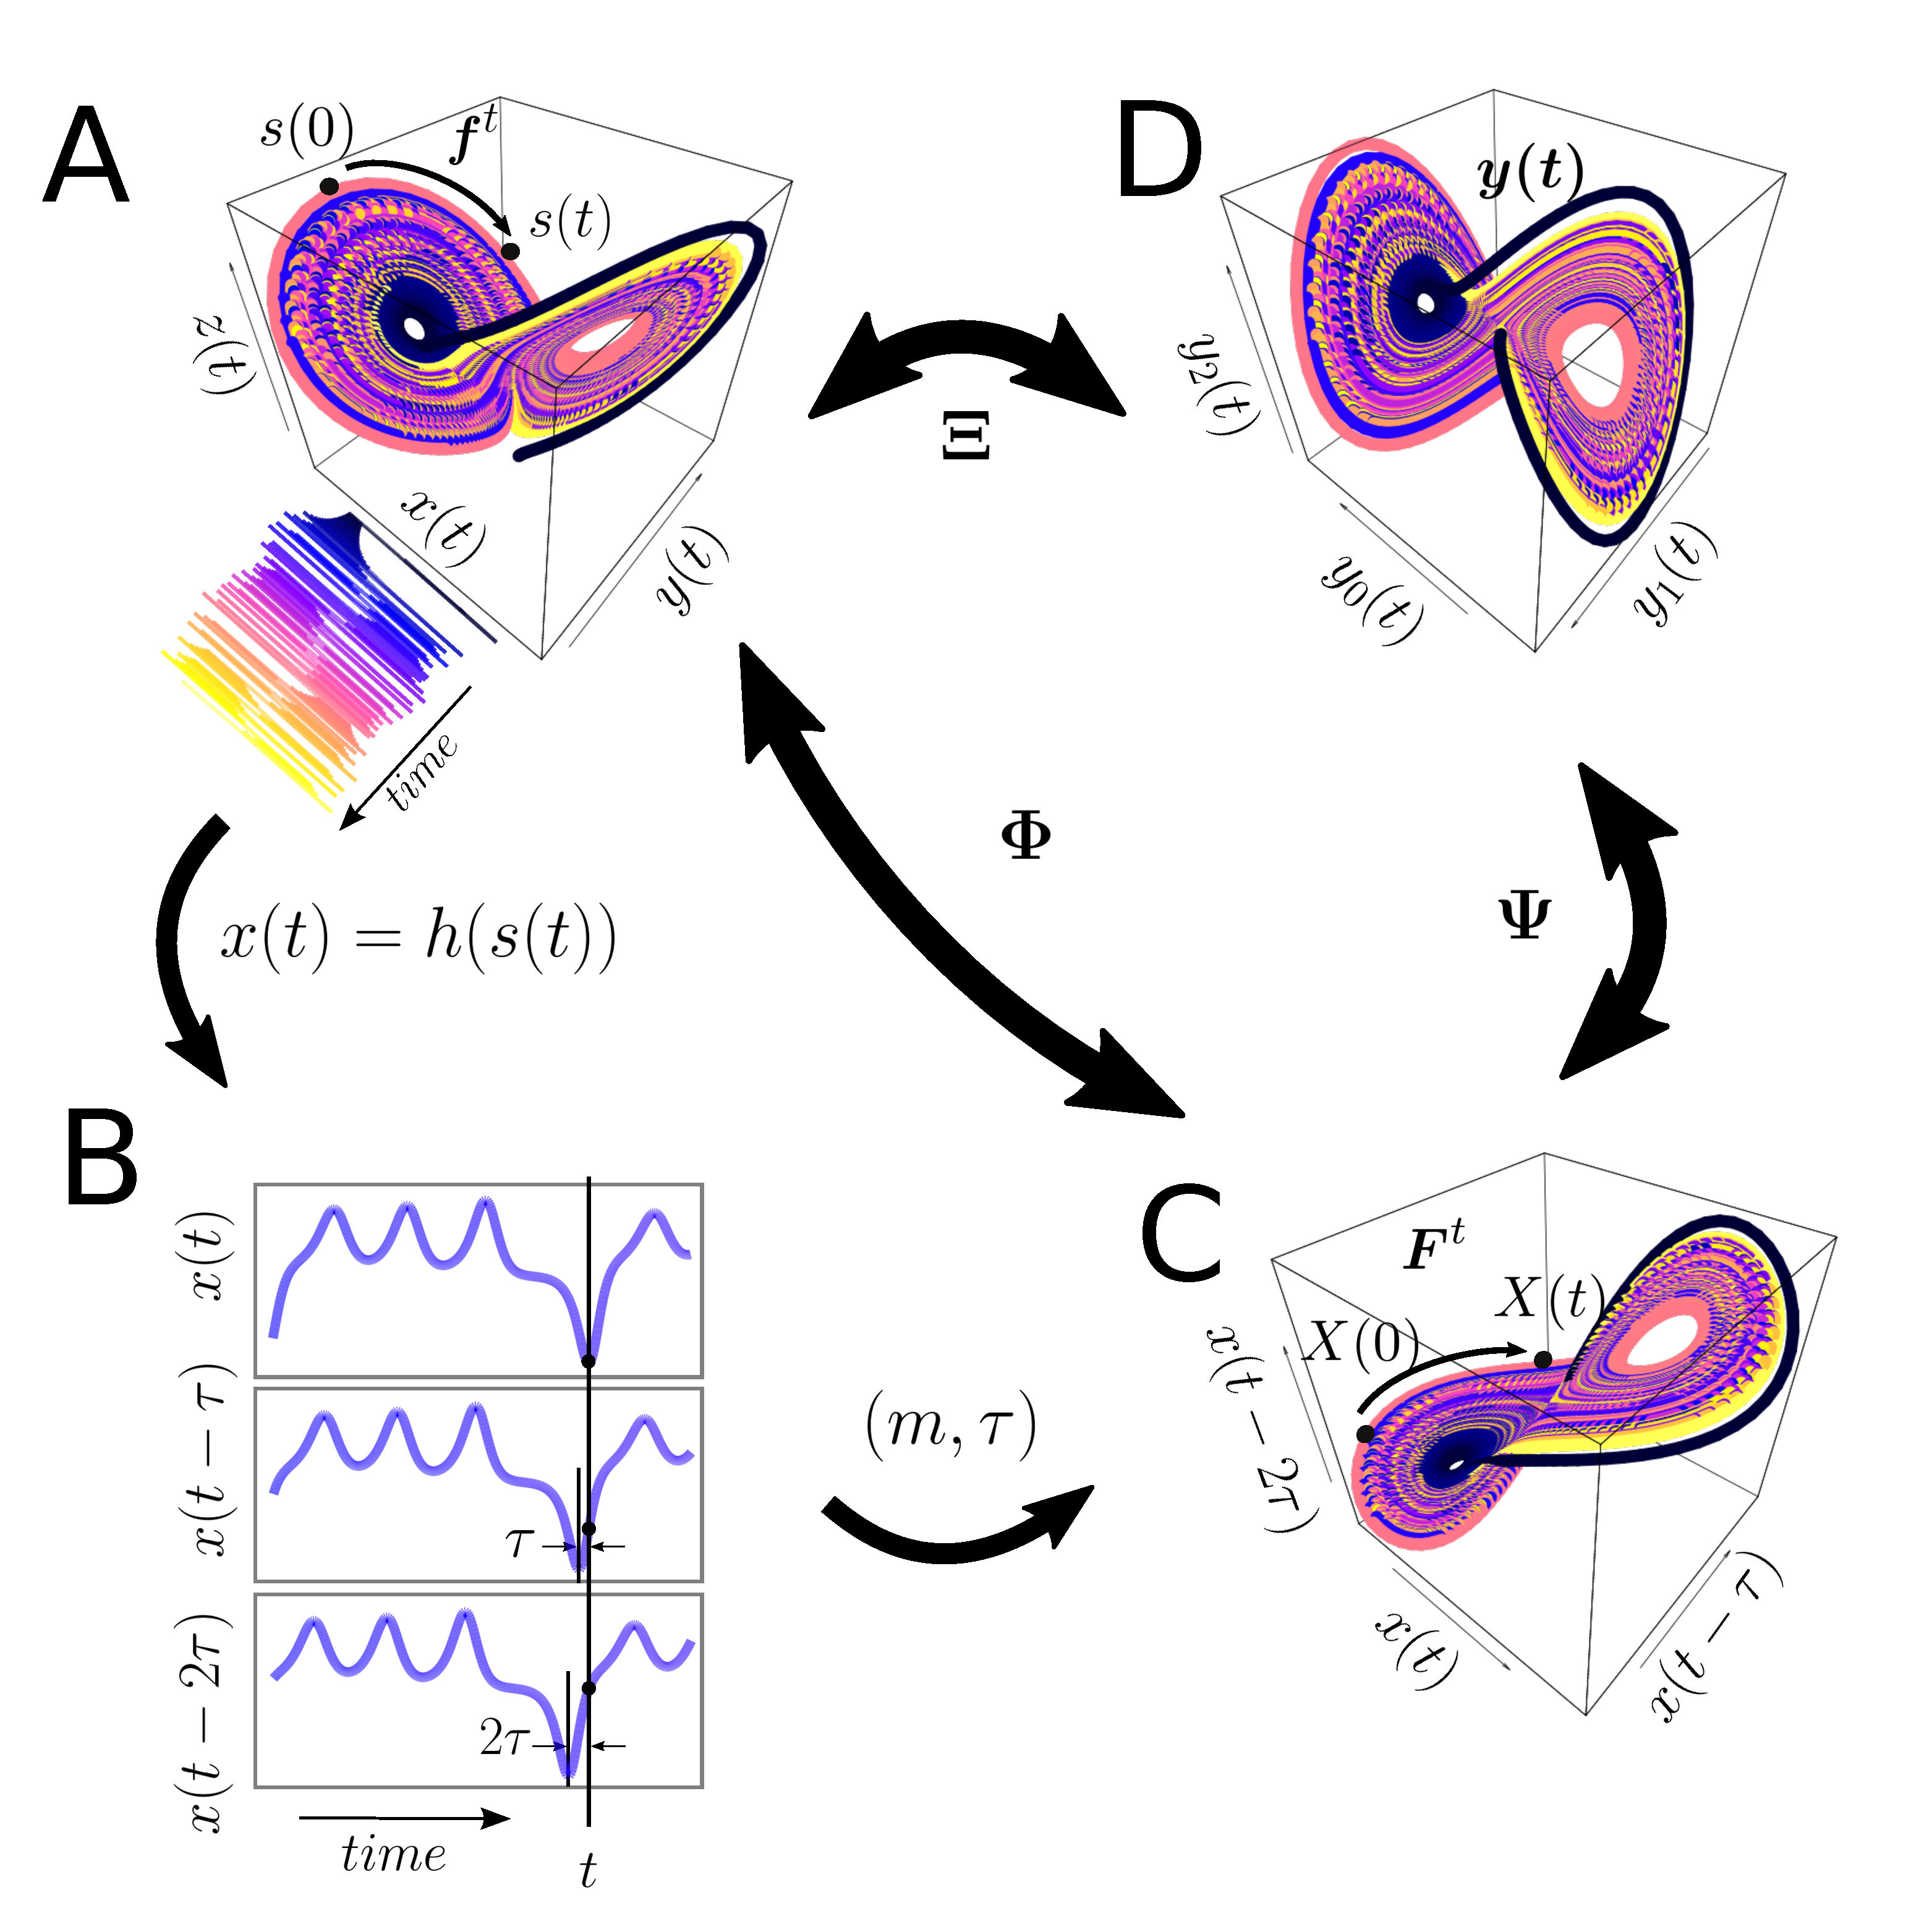
\includegraphics[width=1.0\textwidth]{rss}
    \caption[State space reconstruction methodology]{
	{\bf State space reconstruction methodology.}
	State space reconstruction is based on $x(t)=h[s(t)]= h[f^t [s(0)]]$
	where $h[ ]$ is a function $h: M \rightarrow \mathbb{R}$, defined on 
	the trajectory $s(t)$. $f$ is the true dynamical system, 
	$f:M \rightarrow M$, defined as evolution function and $f^t$, 
	with time evolution $t \in \mathbb{N}$ which is the $t$-th iteration 
	of $f$ that corresponds to an initial position $s(0) \in M $. 
	The time-delay embedding represented as the $\Phi$, maps the original
    	$d-$dimensional state $s(t)$ into the $m-$dimensional uniform 
	time-delay embedding matrix $\boldsymbol{X}(t)$.
	The transformation map $\Psi$ maps $\boldsymbol{X}(t)$ into a 
	new state $y(t)$ of dimensions $n < m$.
	(A) $M-$dimensional state space (e.g. Lorenz system);
    	(B) Delayed copies of $1-$dimensional $x(t)$ from the Lorenz system;
    	(C) $m-$dimensional reconstructed state space with 
	\texorpdfstring{$m$}{m} and    \texorpdfstring{$\tau$}{T}, and 
    	(D) $y(t)$ is the $n-$dimensional reconstructed state space.
	The total reconstruction map is represented as $\Xi = \Psi \circ \Phi $
	where $\Phi$ is the delay reconstruction map and 
	$\Psi$ is the coordinate transformation map.
	This figure is adapted from the work of 
   	\cite{Quintana-Duque2012, casdagli1991, uzal2011}
	and R code to reproduce the figure is available from \cite{hwum2018}.
    }
    \label{fig:ssr}
\end{figure}
%%---------------------------------(FIGURE)-------------------------------------

\section{Uniform Time-Delay Embedding (UTDE)}\label{sec:utimedelayembedding}
\cite{frank2010} and \cite{sama2013} refer to the state space reconstruction 
outlined in \ref{sec:rss} as "time-delay embeddings" or "delay coordinates", 
respectively. However, the term "uniform time-delay embedding" 
is considered as being more descriptive and appropriate terminology 
for this thesis.

The uniform time-delay embedding is represented as a matrix of uniform 
delayed copies of the time series $\{ \boldsymbol{x}_n \}_{n=1}^N$ where $N$ 
is the sample length of $\{ \boldsymbol{x}_n \}$ and $n$ is index for the 
samples of $\{ \boldsymbol{x}_n \}$. $\{ \boldsymbol{x}_n \}_{n=1}^N$ has a 
sample rate of $T$. The delayed copies of $\{ \boldsymbol{x}_n \}$ are 
uniformly separated by $\tau$ and represented as 
$\{\boldsymbol{ \tilde{x} }_{n- i\tau} \}$ where $i$ goes from 
$0,1, \dots, (m-1)$ (Fig~\ref{fig:utde}).
$\{\boldsymbol{ \tilde{x} }_{n- i\tau} \}$ contains information of unobserved 
state variables and encapsulates the information of the delayed copies of 
the available time series in the uniform time-delay embedding matrix 
$\boldsymbol{X}^{m}_{\tau}$, $\boldsymbol{X}^{m}_{\tau} \in \mathbb{R}^m$, 
defined as
%%********************************[EQUATION]************************************
\begin{equation}\label{eq:tde}
\boldsymbol{X}^{m}_{\tau}  =
\begin{pmatrix}
\boldsymbol{ \tilde{x} }_n \\
\boldsymbol{ \tilde{x} }_{n-\tau} \\
\boldsymbol{ \tilde{x} }_{n-2\tau} \\
\vdots \\
\boldsymbol{ \tilde{x} }_{n- (m-1) \tau} \\
\end{pmatrix}^\intercal, 
\end{equation}
%%********************************[EQUATION]************************************
where $m$ is the embedding dimension, $\tau$ is the embedding delay and
$ ^\intercal$ denotes the transpose. $m$ and $\tau$ are known as embedding 
parameters.
%%%********************************[EQUATION]************************************
The matrix dimension of $ \boldsymbol{X}_{\tau}^{m} $ is defined by
$N-(m-1)\tau$ rows and $m$ columns and $N-(m-1)\tau$ defines the length of 
each delayed copy 
of $\{ \boldsymbol{ \tilde{x} }_n \}$ in $\boldsymbol{X}^{m}_{\tau}$.
A graphical representation of uniform time-delay embedding is shown in 
Figure~\ref{fig:utde}. See Appendix \ref{appendix:a} for further details 
and explicit examples of uniform time-delay embedding methodology. 
%---------------------------------(FIGURE)-------------------------------------
\begin{figure}
 \centering
   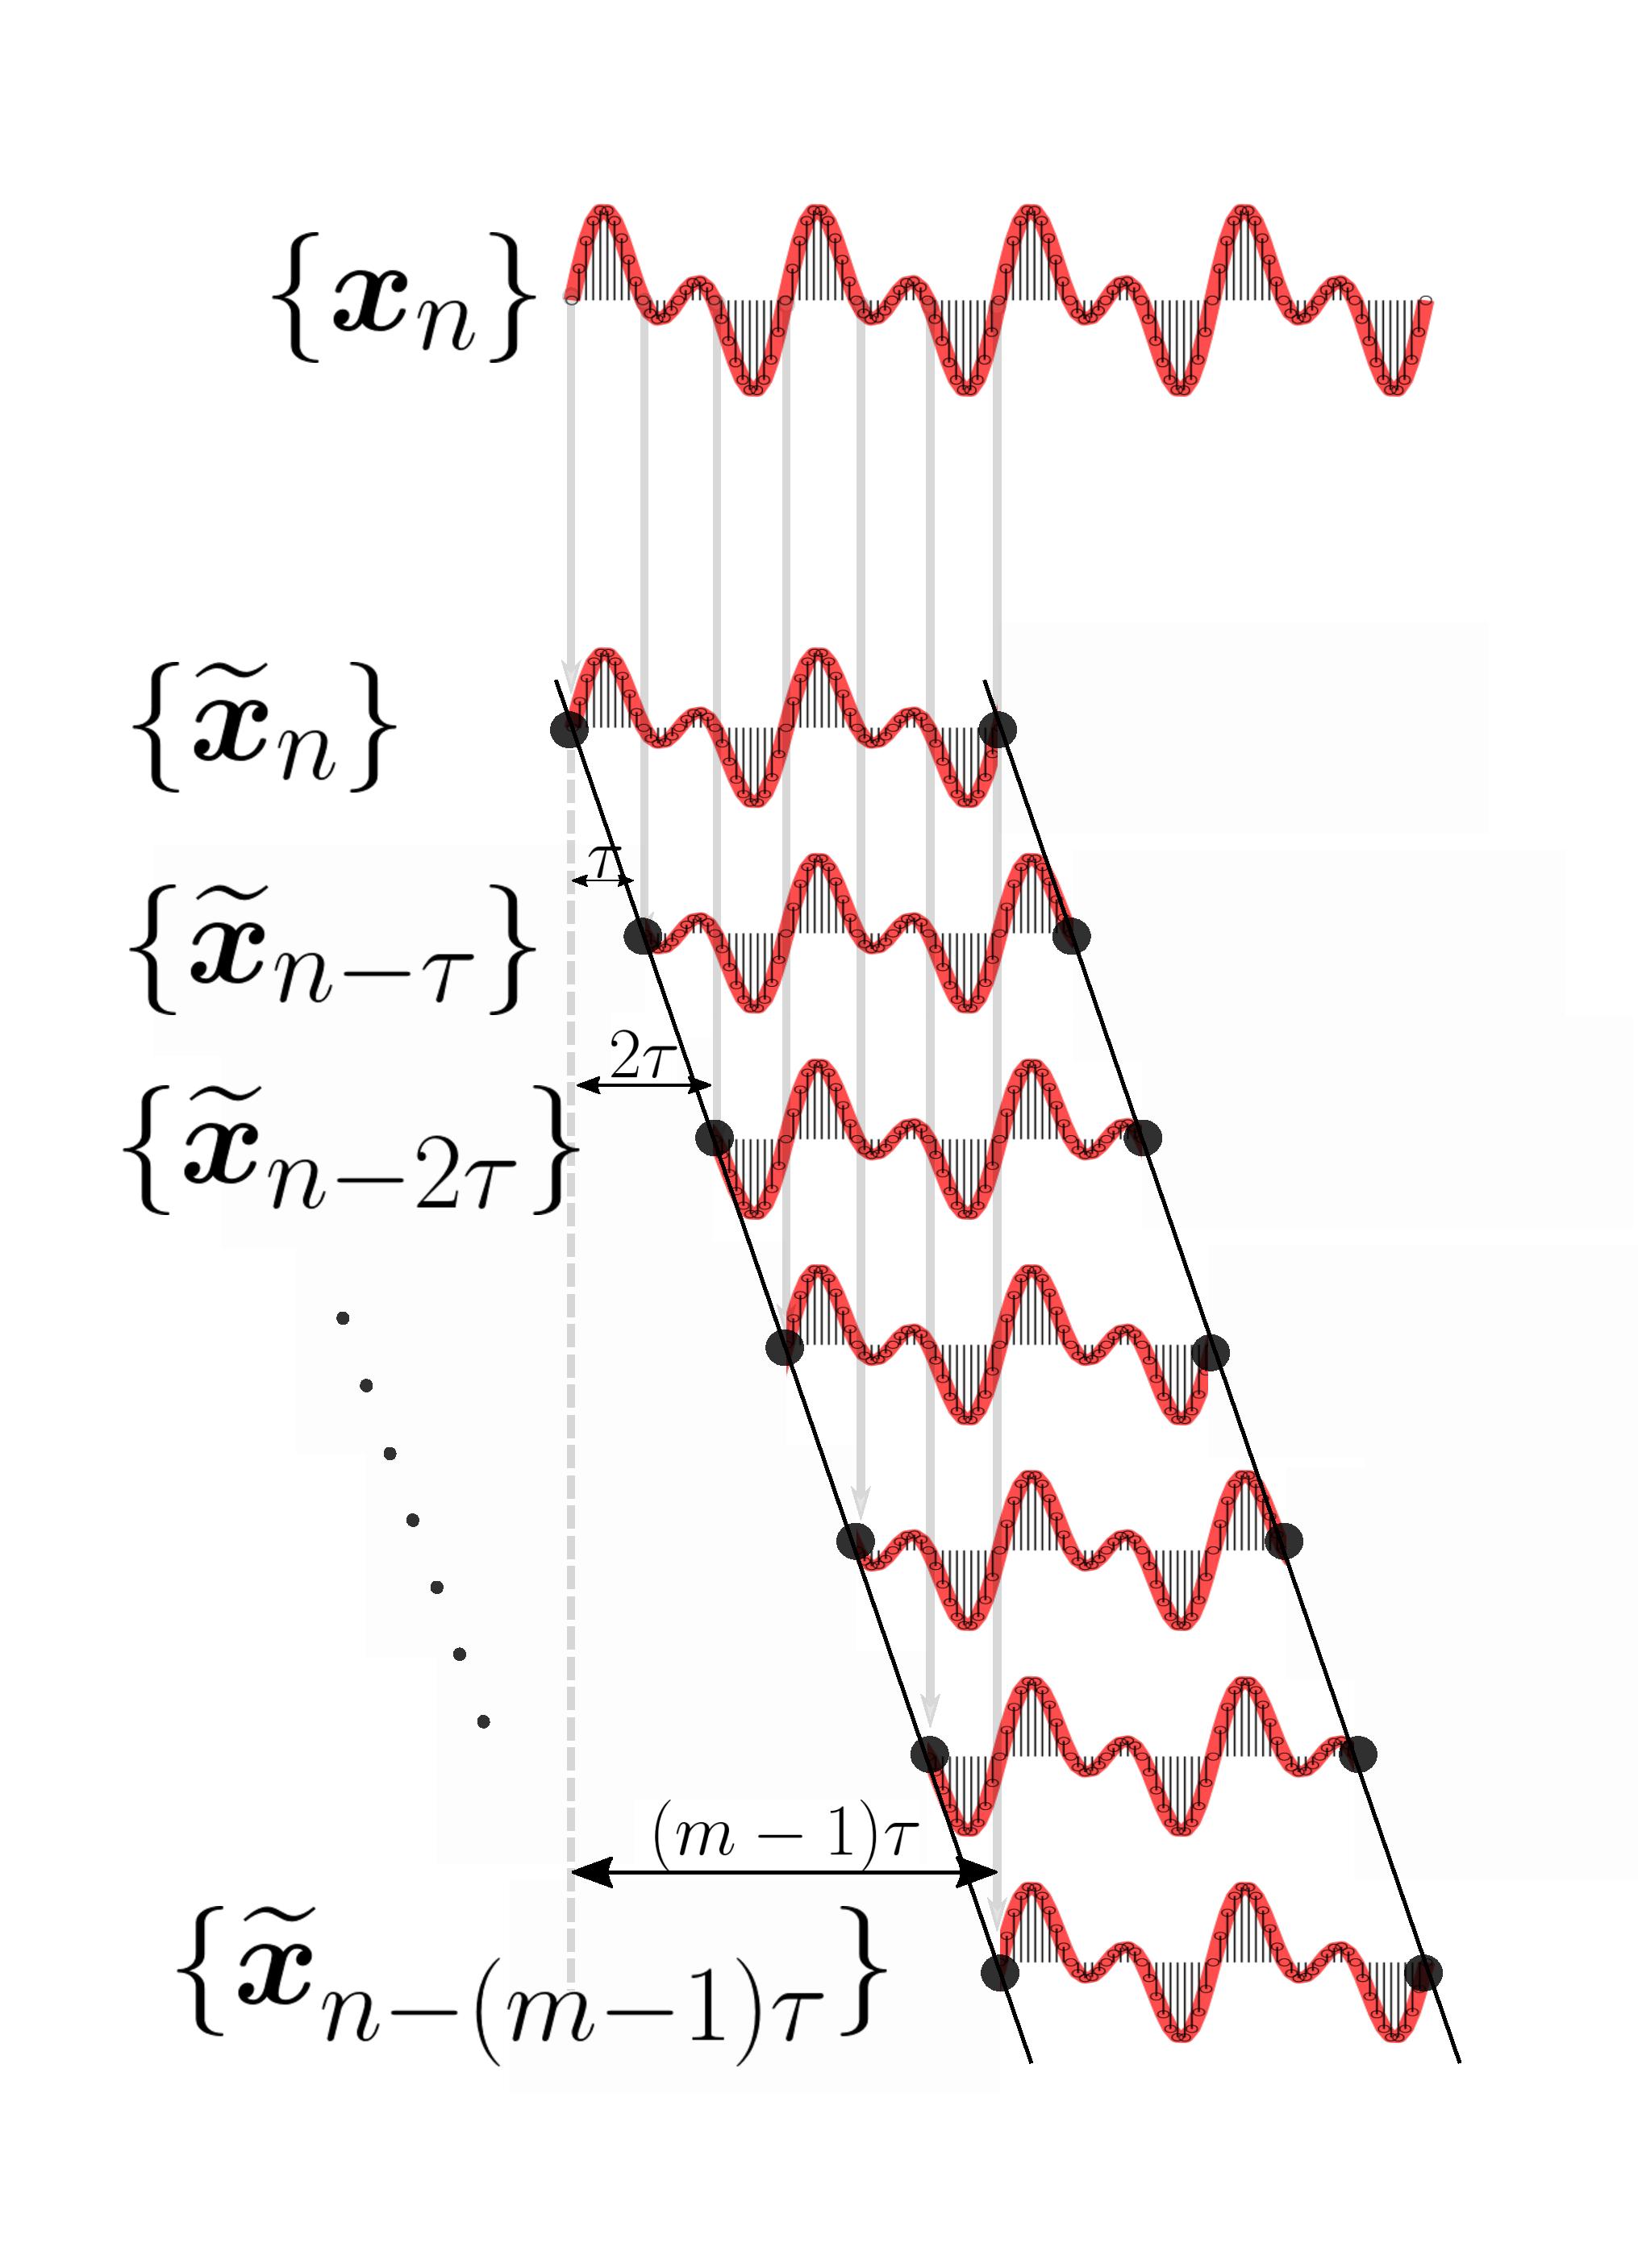
\includegraphics[width=0.95\textwidth]{utde}
   \caption
	[Uniform time-delay embedding]{
	{\bf Uniform time-delay embedding (UTDE).} 
	UTDE is illustrated as $m-1$ delayed copies
   	of $\{ \boldsymbol{x}_n \}$ which is uniformly separated by $\tau$.
	UTDE is represented as
	$\{ \boldsymbol{ \tilde{x} }_n, \dots,  
	\boldsymbol{ \tilde{x} }_{n -(m-1)\tau}   \}$ (Eq.~\ref{eq:tde}).
	R code to reproduce the figure is available \cite{hwum2018}.
   }
   \label{fig:utde}
\end{figure}
%%---------------------------------(FIGURE)-------------------------------------

\section{Estimation of Embedding Parameters}
The estimation of the embedding parameters ($m$ and $\tau$) is an essential 
step for the state space reconstruction in order to apply the method of
uniform time-delay embedding (UTDE). 
Hence, I review two of the most common 
algorithms, which will be used in this thesis, to compute the embedding
parameters: the false nearest neighbour (FNN) and the average mutual 
information (AMI).

\subsection{False Nearest Neighbours (FNN)} \label{ch3:fnn}
To select the minimum embedding dimension $m_0$, \cite{kennel1992}
used the method of false neighbours which can be understood as follows:
on one hand, when the embedding dimension is too small to unfold the attractor
(i.e. evolving trajectories in a state space) 
"not all points that lie close to each other will be neighbours and some points
appear as neighbours as a result of the attractor being projected down into an
smaller space", on the other hand, when increasing the embedding dimension 
"points that are near to each other in the sufficient embedding dimension 
should remain close as the dimension increase from $m$ to $m+1$"
\citep[p. 3]{krakovska2015}.

From a mathematical point of view, state space reconstruction is done when 
the attractor is unfolded with either the minimum embedding dimension, $m_0$, 
or any other embedding dimension value where $m \ge m_0$ \citep{kennel1992}.
In contrast, any large value of $m_0$ leads to excessive computations 
\citep{bradley2015}. Hence, \cite{Cao1997} proposed an algorithm based on the
false neighbour method where only the time-series and one delay embedding value 
are necessary to select the minimum embedding dimension. 
Cao's algorithm is based on $E(m)$, which is the mean value of all $a(i,m)$,
and defined as: 
%%********************************[EQUATION]************************************
\begin{equation}\label{eq:e}
  \begin{aligned}
E(m) &= \frac{1}{N-m\tau} \sum_{i=1}^{N-m\tau} a(i,m) \\
    &=
       \frac{1}{N-m\tau} \sum_{i=1}^{N-m\tau}
       \frac{ || \boldsymbol{X}_i(m+1) - \boldsymbol{X}_{n(i,m)}(m+1) || }
            { || \boldsymbol{X}_i(m) - \boldsymbol{X}_{n(i,m)}(m) ||  }
  \end{aligned}
\end{equation}
%%********************************[EQUATION]************************************
where $\boldsymbol{X}_i(m)$ and $\boldsymbol{X}_{n(i,m)}(m)$ are the time-delay
embeddings with $i=1,2,\dots,N-(m-1)\tau$ and 
$ n(i,m)= 1 \le n(i,m) \le N-m\tau$.
From Eq.~\ref{eq:e} $E(m)$ is only dependent on $m$ and $\tau$ for which 
$E_1(m)$ is defined as
%%********************************[EQUATION]************************************
\begin{equation}\label{eq:e1}
E_1(m) = \frac{ E(m+1) } { E(m)}.
\end{equation}
%%********************************[EQUATION]************************************
$E_1(m)$ is therefore proposed to describe the variation from $m$ to $m+1$
in order to find the minimum embedding dimension $m_0$ (Eq.~\ref{eq:e1}).
As \citealt[p. 44]{Cao1997} described: "$E_1(m)$ stops changing when $m$ is 
greater than some $m_0$, if the time series comes from a multidimensional 
state space then $m_0 + 1$ is the minimum dimension".
Additionally, \cite{Cao1997} proposed $E_2(m)$ to distinguish deterministic 
signals from stochastic signals. $E_2(m)$ is defined as
%%********************************[EQUATION]************************************
\begin{equation}\label{eq:e2}
E_2(m) = \frac{ E^* (m+1) } { E^*(m)},
\end{equation}
%%********************************[EQUATION]************************************
where
%%********************************[EQUATION]************************************
\begin{equation}\label{eq:ee}
E^*(m) = \frac{1}{N-m\tau} \sum_{i=1}^{N-m\tau}
|| \boldsymbol{X}_i(m+1) - \boldsymbol{X}_{n(i,m)}(m+1) ||.
\end{equation}
%%********************************[EQUATION]************************************
For instance, when the signal comes from random noise (values that are 
independent from each other), all $E_2(m)$ values are approximately equal 
to 1 (e.g. $E_2(m) \approx 1$). However, for deterministic data $E_2(m)$ is 
not constant for all $m$ (e.g. $E_2(m) \neq 1$).

As an example of the use of $E_1(m)$ and $E_2(m)$ values, I consider two time 
series: the solution for the $x$ variable  of the chaotic deterministic Lorenz 
system (Figure~\ref{fig:e1e2}E), and a Gaussian noise time series with 
zero mean and a variance of one (Figure~\ref{fig:e1e2}F).
I then compute $E_1(m)$ and $E_2(m)$ values for each time series.
The $E_1(m)$ values for the chaotic time series appear to be constant
after the dimension is equal to six. The determination of six is 
given that any value of $m$ can be used as $E_1(m)$ values are within 
the threshold of $1\pm0.05$ (Fig~\ref{fig:e1e2}A). 
Althought the $E_2(m)$ values for the chaotic time series tend to be closer to
one as $m$ increses, these are different to one (Fig~\ref{fig:e1e2}C), 
for which, it can be concluded that the chaotic time series comes 
from a chaotic deterministic signal.
With regard to the noise time series,  $E_1(m)$ values appeared to be constant
when $m$ is close to thirteen which is defined by the same threshold of 
$1\pm0.05$ (Figure~\ref{fig:e1e2}B). 
Then, contrary to the $E_2(m)$ values for a chaotic 
Lorenz time series, all values of $E_2(m)$ for a noise time series are 
approximately equal to one (Figure~\ref{fig:e1e2}D). 
Hence, $E_1(m)$ values then indicate the minimum 
embedding dimension of the noisy time series is thirteen, however all of 
the $E_2(m)$ values are approximately equal to one (Figure~\ref{fig:e1e2}D)
for which it can be concluded that noise time series is a stochastic signal.
%%---------------------------------(FIGURE)-------------------------------------
\begin{figure}[!h]
  \centering
  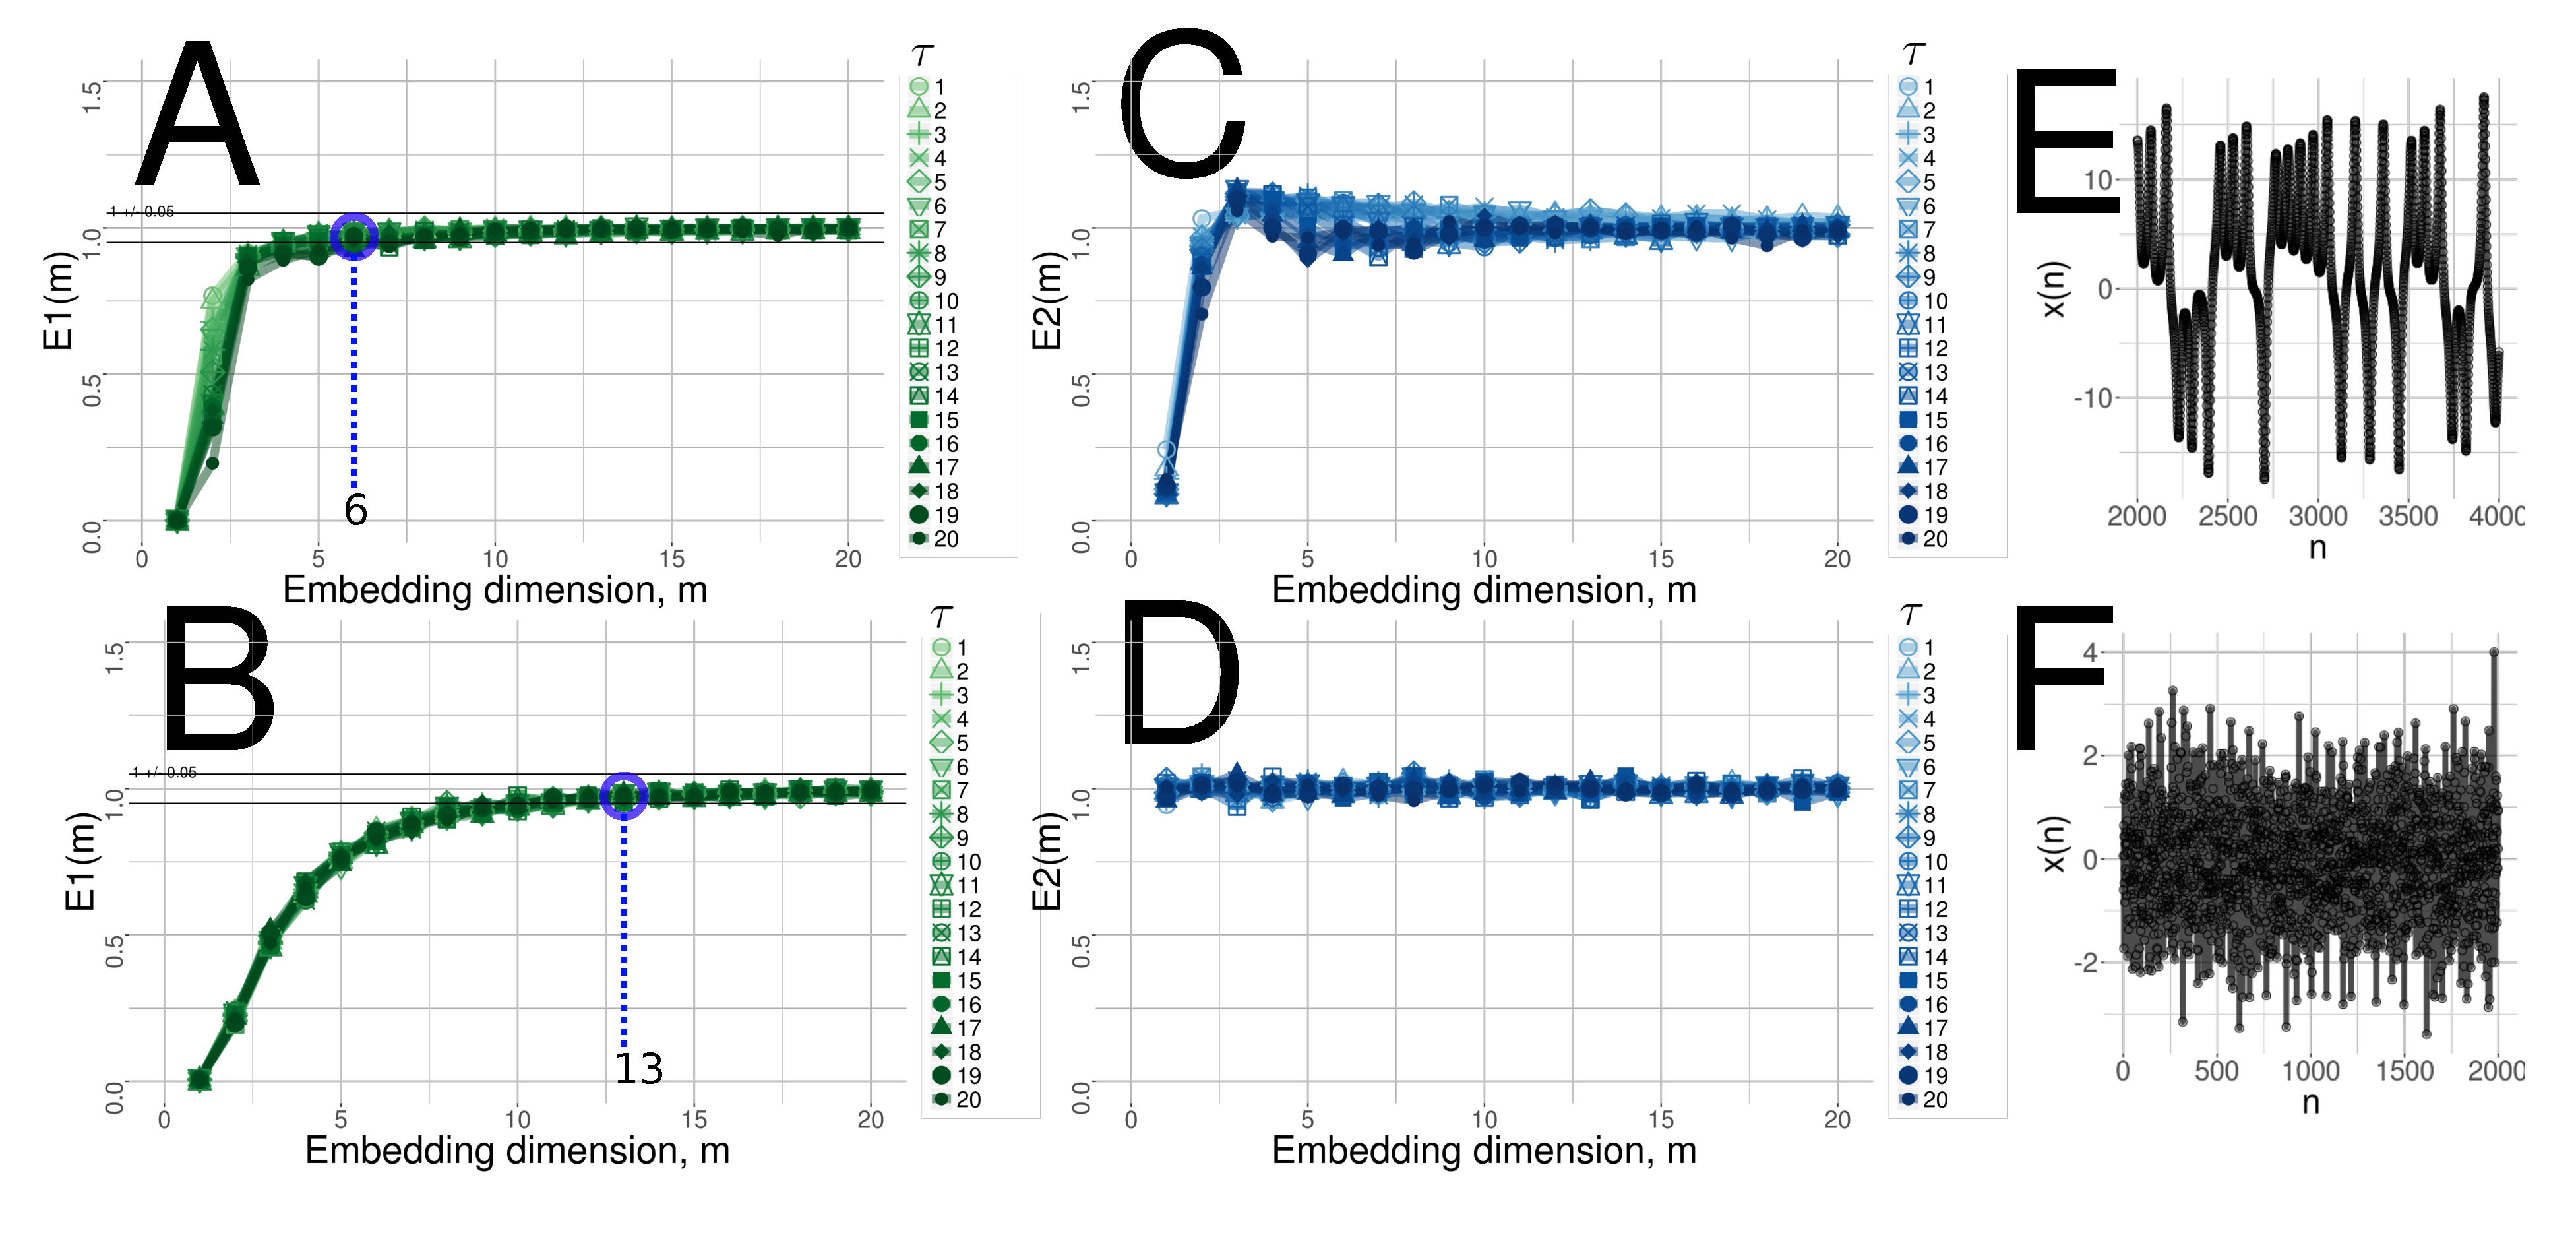
\includegraphics[width=1.0\textwidth]{cao}
    \caption
	[Minimum dimension embedding values with Cao's method]{
	{\bf Minimum dimension embedding values with Cao's method.} 
	(A, B) $E_1 (m)$ values and (C, D) $E_2(m)$ values 
	with variations of $\tau$ values from one to twenty
	for (E) chaotic and (F) random time series.
	R code to reproduce the figure is available from \cite{hwum2018}.
        }
    \label{fig:e1e2}
\end{figure}
%%---------------------------------(FIGURE)-------------------------------------

It is important to note that for this thesis not only the values for 
$E_1(m)$ and $E_2(m)$ are computed but also a variation of $\tau$ from 
1 to 20 (Figure~\ref{fig:e1e2} (A,B,C,D)) has been explored. 
The purpose of using variations for $\tau$ is to show its independence 
with regard to the $E_1(m)$ (Fig. \ref{fig:e1e2}(A,B))
and $E_2(m)$ (Fig. \ref{fig:e1e2}(C,D)).
Although \cite{Cao1997} mentioned that no parameters are required to find
the minimum embedding dimension, I found that it is necessary to define a  
threshold for which $E_1(m)$ values appear to be constant. 
Hence, for the given examples and the reported results for this thesis, 
I defined a threshold to be 0.05 
(see Fig. \ref{fig:e1e2}(A) with the parallel lines of the threshold 
near to one $1\pm0.05$).

\subsection{Average Mutual Informationi (AMI)}
When selecting the delay dimension parameter, $\tau$, one can consider the 
following two cases:
(i) when $\tau$ is too small, the elements of time-delay embedding will be 
along the bisectrix of the phase space and the reconstruction is generally 
not satisfactory, 
(ii) when $\tau$ is too large the elements of the uniform 
time-delay embedding will become spread and uncorrelated which makes 
recovering the underlying attractor (i.e. evolving trajectories in a 
state space) difficult if not impossible 
\citep{casdagli1991, emrani2014a, garcia2005e71}.

There are many approaches to compute the embedding parameters 
\citep{bradley2015}, for instance, geometry-based methodologies where 
the amount of space filled in the reconstructed state is the metric to 
compute the delay embedding \citep{mrosenstein1994} or 
theoretical approaches to estimate an optimal parameter for 
$\tau$ \cite{casdagli1991}. 
However, the autocorrelation function and the average mutual information 
(AMI) are the two most commonly used algorithms to compute the minimum 
delay embedding parameter $\tau_0$. \cite{emrani2014a} used the 
autocorrelation function in which the first zero crossing is considered 
as the minimum delay embedding parameter. However, the autocorrelation 
function is a linear statistic whereas AMI considers the nonlinear 
dynamical correlations \citep{afraser1986,krakovska2015}.
With that in mind, the AMI algorithm is described below to estimate 
the minimum delay embedding parameter, \texorpdfstring{$\tau_0$}{T}.

To compute the AMI, an histogram of $x(n)$ using $n$ bins is calculated
and then a probability distribution of data is computed \citep{kantz2003}.
AMI is therefore denoted by $I(\tau)$ which is the average mutual 
information between the original time series, $x(n)$, and the delayed time 
series, $x(n-\tau)$, delayed by $\tau$ \citep{kabiraj2012}. AMI is defined by
%%********************************[EQUATION]************************************
\begin{equation}\label{eq:ami}
I(\tau) = \sum_{i,j}^N p_{ij} \log_2 \frac{ p_{ij} }{ p_i p_j }.
\end{equation}
%%********************************[EQUATION]************************************

Probabilities are defined as follows: 
$p_i$ is the probability that $x(n)$ has a value inside the $i$-th bin of 
the histogram, $p_j$ is the probability that $x(n+\tau)$ has a value inside 
the $j$-th bin of the histogram and $p_{ij}(\tau)$ is the probability 
that $x(n)$ is in bin $i$ and $x(n+\tau)$ is in bin $j$.
The AMI is measured in bits (base 2, also called shannons) 
\citep{kantz2003, nonlinearTseries2016}.
For small $\tau$ ($\tau < 3$), AMI will be large ( $I(\tau)>6$)and as 
$m$ increase AMI will then decrease rapidly. Hence, as $\tau$ increase 
and goes to a large limit, $x(n)$ and $x(n+\tau)$ have 
nothing to do with each other and $p_(ij)$ is factorised as $p_ip_j$ for 
which AMI is close to zero.  Then, in order to obtain $\tau_0$, 
"it has to be found in the first minimum of $I(\tau)$ where $x(n+\tau)$ 
adds maximal information to the knowledge from $x(n)$" meaning that the 
redundancy between $x(n+\tau)$ and $x(n)$ is the least
\citep[p. 151]{kantz2003}.

%%---------------------------------(FIGURE)-------------------------------------
\begin{figure}[!h]
  \centering
  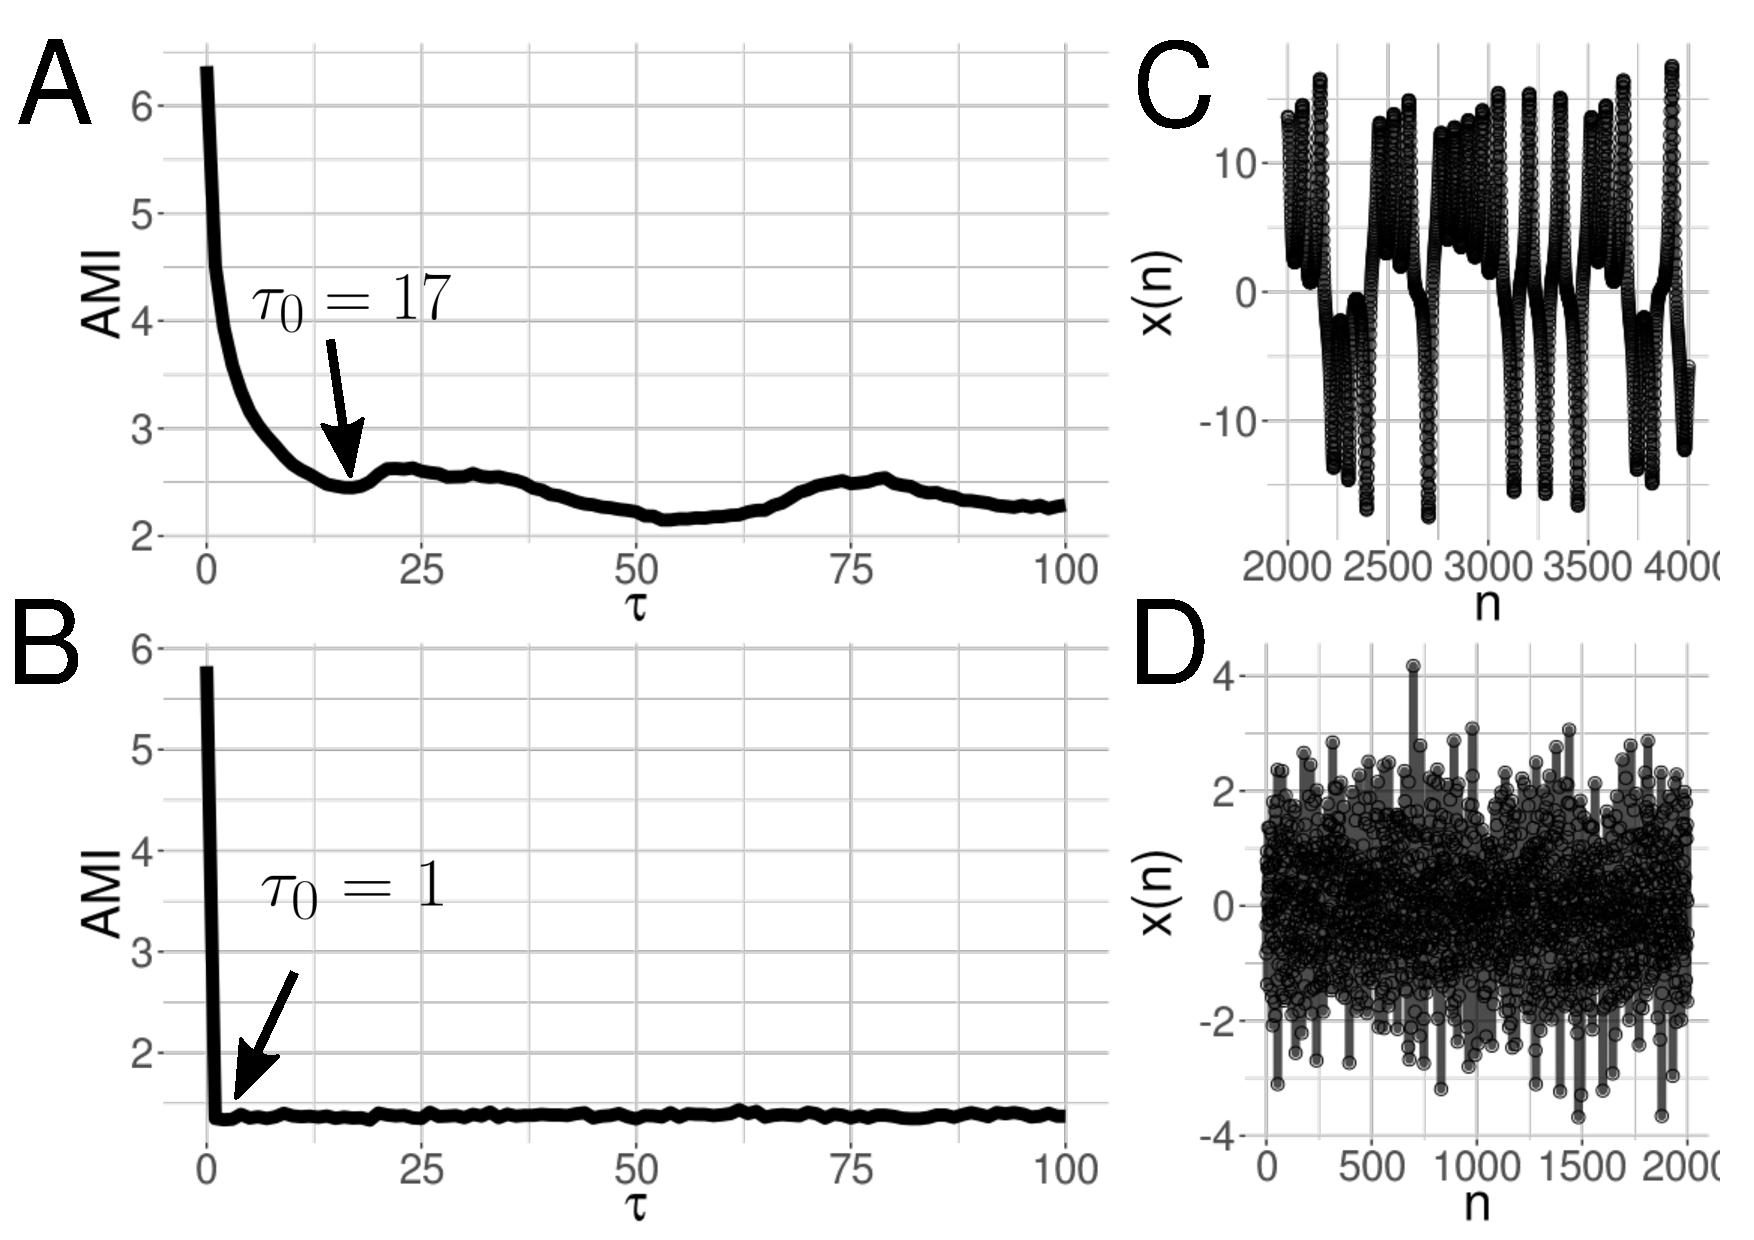
\includegraphics[width=0.7\textwidth]{ami}
    \caption
	[Minimum delay embedding values with AMI's method]{
	{\bf Minimum delay embedding values with AMI's method.} 
    	(A, B) AMI values where its first minimum value in the curve
	is the minimum time delay embedding ($\tau_0$), 
	for (C) a chaotic and (D) noise time series.
	R code to reproduce the figure is available from \cite{hwum2018}.
        }
    \label{fig:amis}
\end{figure}
%%---------------------------------(FIGURE)------------------------------------
For example, I compute the AMI for two time series:
(i) the $x$ solution of the deterministic chaotic Lorenz system, and 
(ii) a noise time series using a normal distribution with mean zero and 
standard deviation equal to one. The AMI plots are shown in 
Figure~\ref{fig:amis}, where the minimum delay embedding parameter for 
the chaotic time series is $\tau_0=17$ and for the noise time series is  
$\tau_0=1$. Hence, it can be concluded that the amount of knowledge for 
any noise time series is zero for which the first minimum embedding 
parameter is equal to one. On the contrary, the first minimum of the AMI 
for the chaotic time series is $\tau_0=17$ which is the value that maximize 
the independence in the reconstructed state space \citep{bradley2015}.

\subsection{Overall minimum embedding parameters} \label{sec:overall_minMT}
The method to select minimum embedding parameters ($m_0$ and $\tau_0$) 
for this thesis is firstly to compute $m_0$ with FNN algorithm 
(considering a threshold of 0.05 for $E_1(m)$ values) and secondly
to compute $\tau_0$ with AMI (which does not need any extra parameter).
From the previous example of the deterministic-chaotic 
Lorenz system, Fig \ref{fig:e1e2}(A) is used to determine 
the minimum dimension embedding ($m_0 =6$) and 
Fig \ref{fig:amis}(A) is used to determine the minimum delay embedding 
($\tau_0 =17$).
Therefore, with the computation of the minimum embedding parameters, the 
reconstructed attractor is created in order to ensure with $\tau_0$ the 
maximum independence between $x(t)$ and $x(t+\tau_0)$ and with $m_0$ 
allowing the trajectories in the reconstructed state space to be unfolded.

As time-series data for this thesis are multidimensional 
(i.e. more than one time series), sample mean 
of individual minimum values $m_{0_i}$ and $\tau_{0_i}$  
is used to get an 
overall value of embedding minimum embedding parameters
$\overline{m}_0$ and $\overline{\tau}_0$ (Eqs. \ref{eq:smmo} and \ref{eq:smto}): 
%, in which 
%are averaged over $N$:
%which is the total number of minimum embedding values:
%%********************************[EQUATION]************************************
\begin{equation} \label{eq:smmo}
	\overline{m}_0= \frac{1}{N} \sum^{N}_{i = 1} m_{0_i},
\end{equation}
%%********************************[EQUATION]************************************
and 
%%********************************[EQUATION]************************************
\begin{equation} \label{eq:smto}
	\overline{\tau}_0= \frac{1}{N} \sum^{N}_{i = 1} \tau_{0_i}, 
\end{equation}
%%********************************[EQUATION]************************************
where $N$ is the number of time series and $i=1,\dots, N$.

It is also important to mention that a maximum of individual minimum 
dimension embeddings, $m_{0_i}$, can be used instead of the overall 
sample mean of individual minimum dimension embeddings. The rationale
for that is because the maximum value can unfold trajectories 
in the reconstructed state space that require a lower embedding 
dimension value. However such statement might be different 
for the maximum of individual minimum embedding delay as such 
maximum might not create the maximum independence 
between $x(n)$ and $x(n+\tau)$ for multiple time-series data. 
See Chapter \ref{chapter7} for future research on optimal embedding 
parameters.

\section{Reconstructed State Space with UTDE} \label{sec:rsswithUTDE}
Given a time series $x(n)$, the UTDE matrix is computed with its 
minimum embedding parameters and then PCA is applied in order to select 
the first three axis of the rotated data to create the reconstructed 
state spaces \citep{frank2010, sama2013}.
See Fig. \ref{fig:ssr} that illustrates and describes the method of 
reconstructed state space with UTDE.

\section{Recurrence Plots (RP)}
Henri Poincar\'e in 1890 introduced the concept of recurrences in 
conservative systems, however the discovery was not put into practice until 
the development of faster computers \citep{marwan2007}, for which 
\cite{eckmann1987} introduced a method where recurrences in the dynamics of 
a system can be visualised.
The intention of \cite{eckmann1987}  was to propose a tool,
called Recurrence Plot (RP), that provides insights into high-dimensional 
dynamical systems where trajectories are very difficult to visualise.
Hence, "RP is a tool that helps us to investigate the 
$m-$dimensional phase space trajectories through a two-dimensional 
representation of its recurrences" \citep[p. 7]{marwan2015}.
Similarly, \cite{marwan2015} pointed out that in addition to the 
methodologies of the state space reconstruction and other dynamic invariants 
(e.g. Lyapunov exponent, Kolmogorov-Sinai entropy), the recurrences of the 
trajectories in the phase space can provide important clues to characterise 
the underlying process for periodicities (as Milankovitch cycles) or 
irregular cycles (as El Ni\~no Southern Oscillation). 
Such recurrences can not only be visualised using Recurrence Plots (RP) 
but also be quantified with Recurrence Quantification Analysis (RQA) metrics, 
which leads to applications of these tools in various areas such as Economics, 
Physiology, Neuroscience, Earth Science, Astrophysics and Engineering 
\citep{marwan2007}.

A recurrence plot based on time series $\{ \boldsymbol{x}_n \}$ is computed 
from the state space reconstruction with uniform time-delay embedding method 
$X(i)=\{ \boldsymbol{ \tilde{x} }_n, \dots,  
\boldsymbol{ \tilde{x} }_{n -(m-1)\tau} \}$
where $i=1,\dots,N$, $N$ is the number of considered states of $X(i)$ 
and $X(i) \in \mathbb{R}^m$ \citep{eckmann1987}.
%Then, one plots a black dot at each point $(i,j)$ in the recurrence plot
%for which $X(j)$ is in the ball of radius $\epsilon$ centred at $X(i)$ 
The recurrence plot is therefore a two-dimensional $N \times N$ square matrix, 
$\mathbf{R}$, where a black dot is placed at $(i,j)$ whenever $X(i)$ is 
sufficiently close to $X(j)$: 
%%********************************[EQUATION]************************************
\begin{equation}
\mathbf{R}^{m}_{i,j} (\epsilon) = 
	\Theta ( \epsilon_i - || X(i) - X(j) ||, \quad 
	X(i) \in \mathbb{R}^m, \quad i,j=1,\dots,N,
\end{equation}
%%********************************[EQUATION]************************************
where $N$ is the number of considered states of $X(i)$, $\epsilon$ is a 
threshold distance, $|| \cdotp ||$ a norm, and $\Theta(\cdotp)$ is the 
Heaviside function (i.e. $\Theta(x)=0$, if $x<0$, and $\Theta(x)=1$ otherwise) 
(Fig~\ref{fig:mrp}) \citep{eckmann1987, marwan2007,marwan2015}.
RP is also characterised with a line of identity (LOI) which is a black main 
diagonal line due to $ R_{i,j}=1 (i,j=1,\dots,N)$. 
%%---------------------------------(FIGURE)-------------------------------------
\begin{figure}[!h]
  \centering
    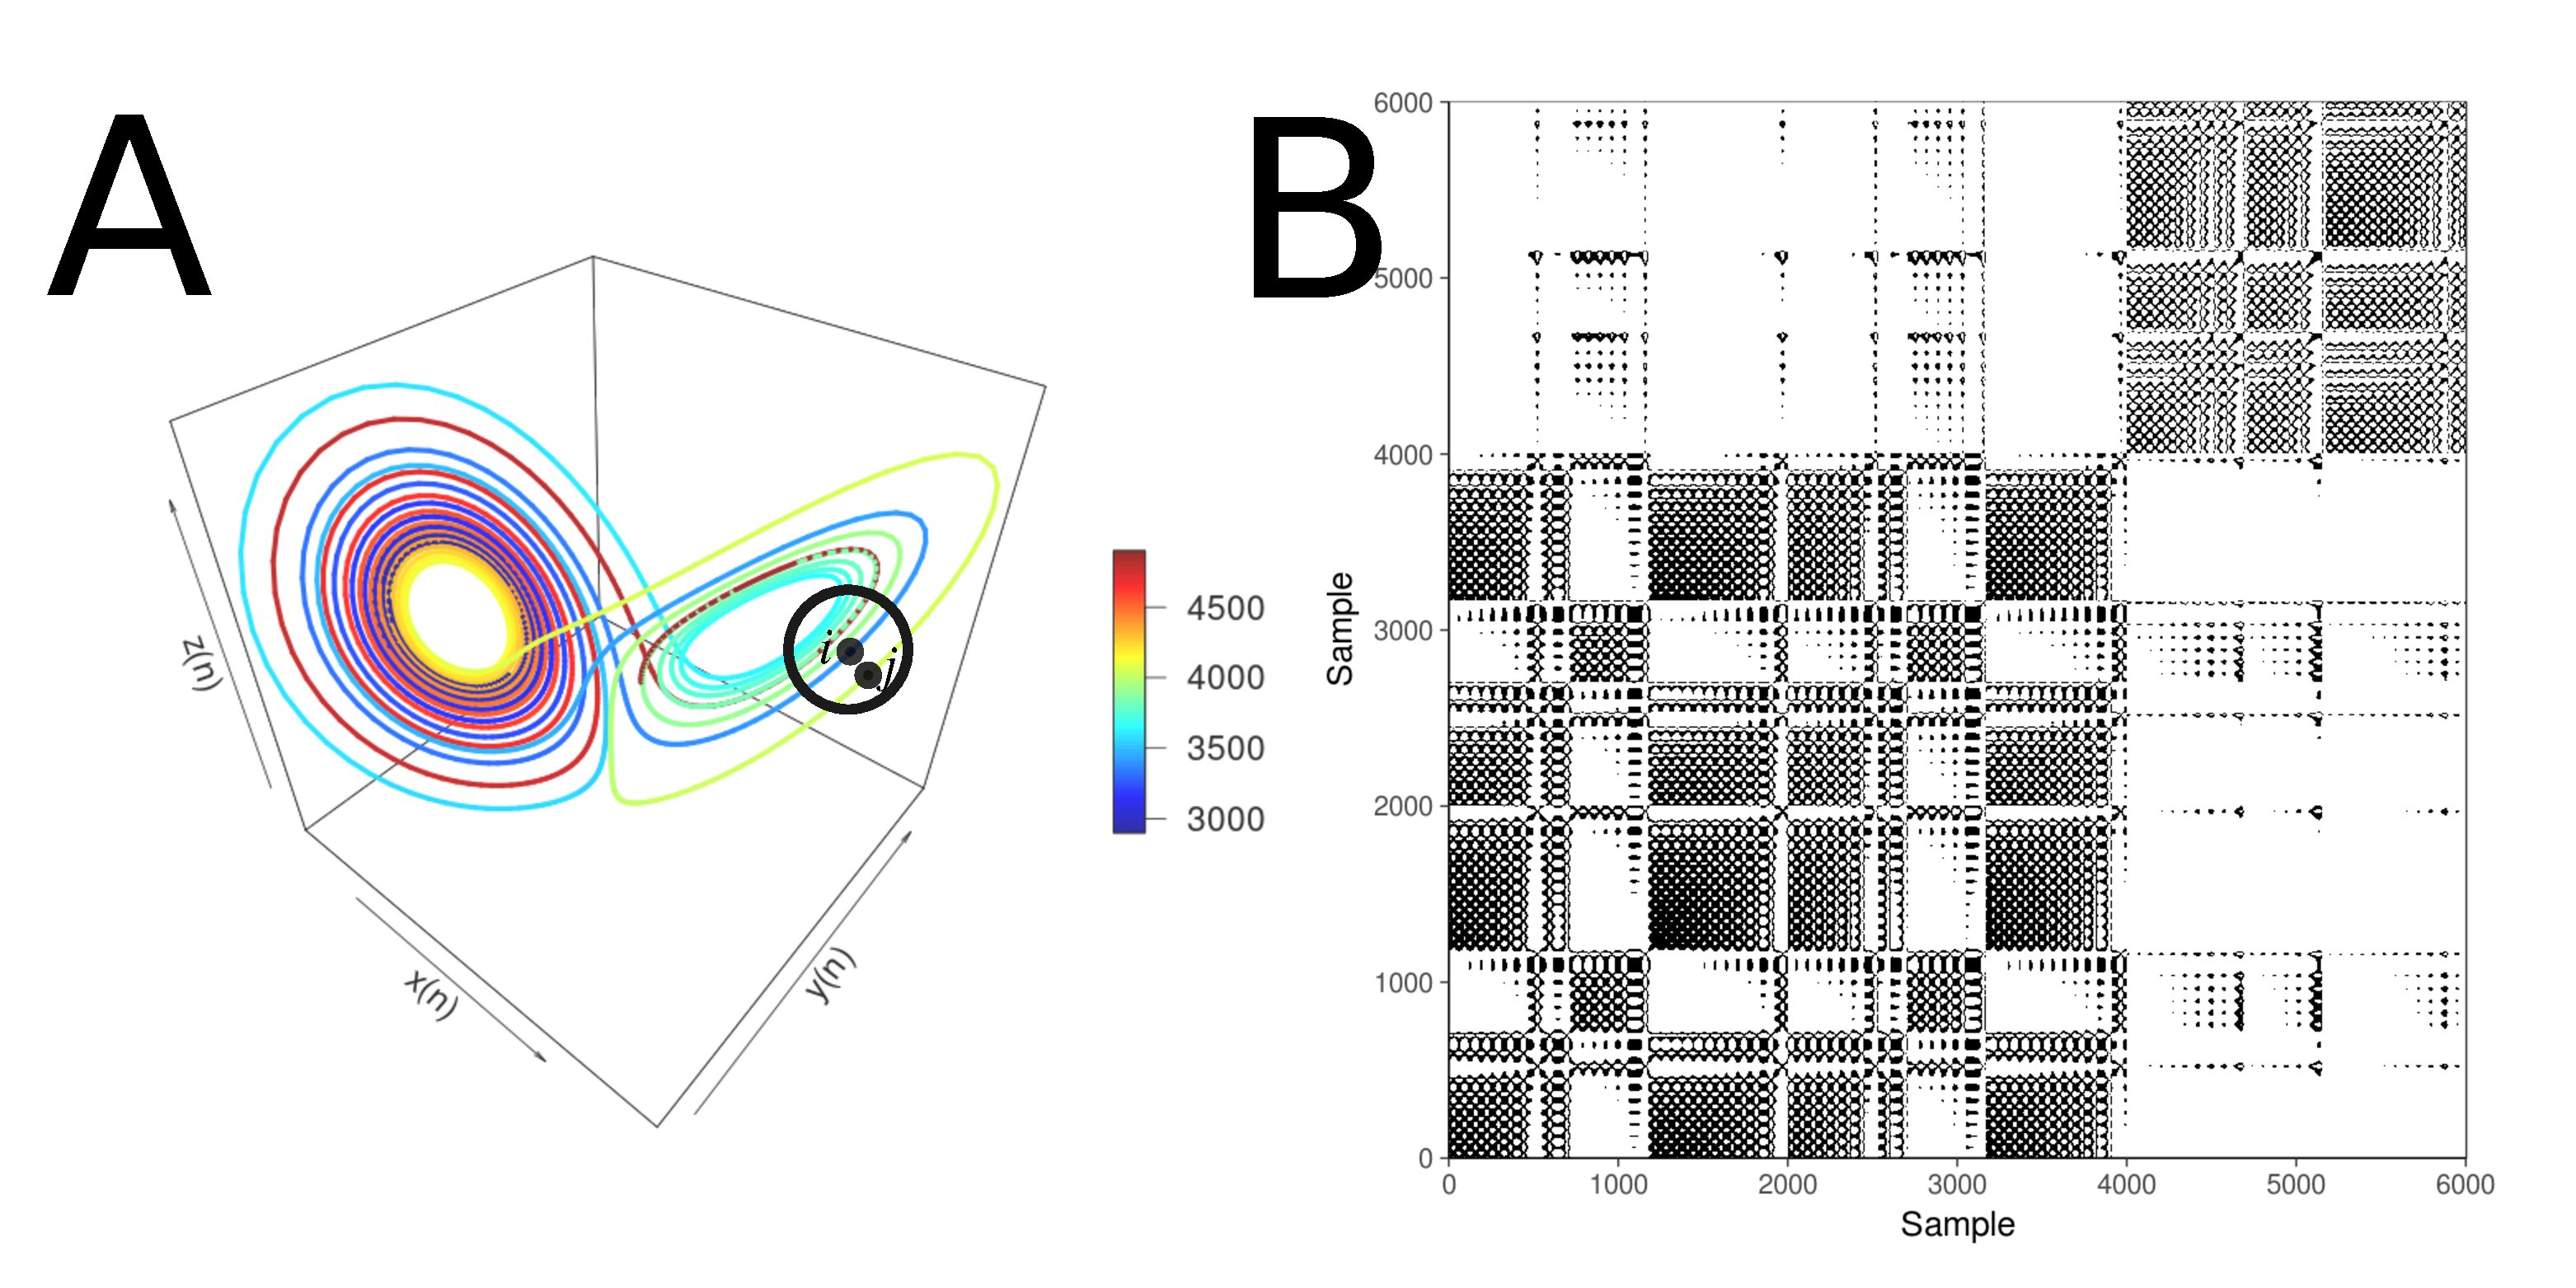
\includegraphics[width=1.0\textwidth]{rp}
    \caption
	[Recurrence Plots]{
	{\bf Recurrence Plots.} 
	(A) State space of the Lorenz system with controlling parameters 
	($\rho=28, \sigma=10, \beta=8/3$). A point, $j$, in trajectory $X()$ 
	which falls into the neighborhood (black circle) of a given point 
	at $i$ is a recurrent point and is represented as a black dot in 
	the recurrence plot at location $(i, j)$ or white otherwise.
	(B) Recurrence plot using the three components of the Lorenz 
	system and the RP with no embeddings and threshold $\epsilon=5$.
	This figure is adapted from \cite{marwan2015} and R code to 
	reproduce it is available from \cite{hwum2018}.
	}
    \label{fig:mrp}
\end{figure}
%%---------------------------------(FIGURE)-------------------------------------

\subsection{Structures of Recurrence Plots}
Pattern formations in RPs can be designated either 
as topology for large-scale patterns or texture for small-scale patterns.
In the case of topology, the following pattern formations are presented:
(i) homogeneous where uniform recurrence points are spread in the RP e.g., 
uniformly distributed noise (Figure~\ref{fig:rp2}A), 
(ii) periodic and quasi-periodic systems where diagonal lines and 
checkerboard structures represent oscillating systems, e.g., sinusoidal 
signals (Figure~\ref{fig:rp2}B), 
(iii) drift where paling or darkening recurrence points away from 
the LOI is caused by drifting systems, 
e.g., logistic map (Figure~\ref{fig:rp2}C), and
(iv) disrupted where recurrence points are presented white areas or 
bands that indicate abrupt changes in the dynamics, e.g. Brownian motion 
(Figure~\ref{fig:rp2}D) \citep{eckmann1987, marwan2015}.
Texture, for small-scale patterns, can be categorised as:
(i) single or isolated recurrence points that represent rare occurring 
states, do not persist for any time or fluctuate heavily,
(ii) dots forming diagonal lines where the length of the small-scale parallel 
lines in the diagonal are related to the ratio of determinism or 
predictability in the dynamics of the system, and
(iii) dots forming vertical and horizontal lines where the length of the 
lines represent a time length where a state does not change or change very 
slowly and the patterns formation represent discontinuities in the signal, and
(iv) dots clustering to inscribe rectangular regions which are related 
to laminar states or singularities \citep{marwan2015}.

%%---------------------------------(FIGURE)-------------------------------------
\begin{figure}
  \centering
    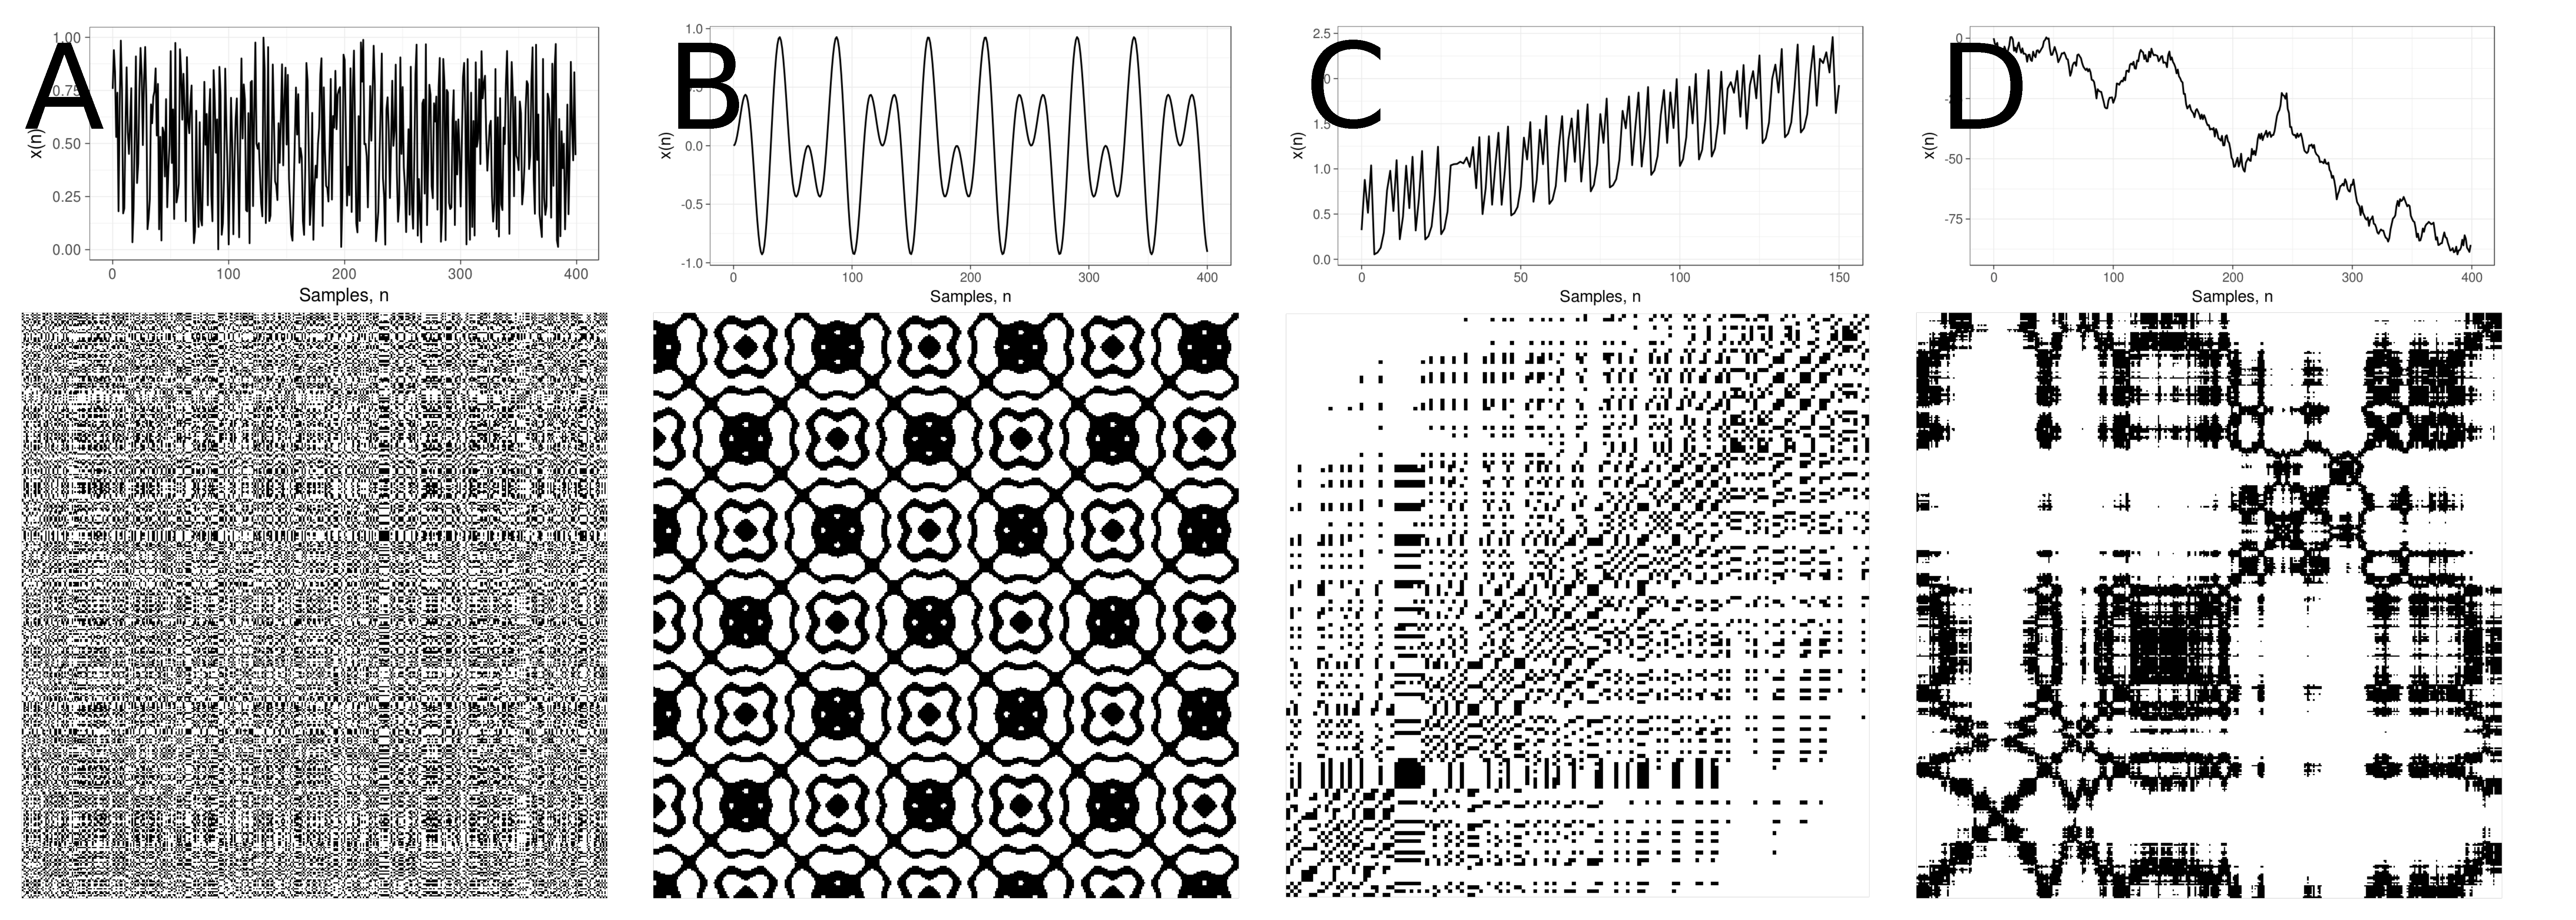
\includegraphics[width=1.0\textwidth]{rpsp}
    \caption
	[Patterns in Recurrence Plots]{
	{\bf Patterns in Recurrence Plots.} 
	Time-series with its respective recurrence plots for:
	(A) uniformly distributed noise,
	(B) super-positioned harmonic oscillation 
	($\sin{ \frac{1}{5} t} \sin{ \frac{5}{100}t) }$),
	(C) drift logistic map ($x_{i+1} = 4 x_i (1- x_i) $) corrupted 
	with a linearly increase term ($0.01 i$), and
	(D) disrupted brownian motion  ($x_{i+1} = x_i + 2rnorm(1) $).
	Figure is adapted from \cite{marwan2015} and R code to reproduce 
	the figure is available from \cite{hwum2018}.
	}
    \label{fig:rp2}
\end{figure}
%%---------------------------------(FIGURE)-------------------------------------

Although, the previous pattern descriptions of the structures in the 
RP offer an idea of the characteristics of dynamical systems from 
time-series, these descriptions might be misinterpreted and conclusions might 
tend to be subjective as these require the interpretation of a researcher(s).
Because of that, recurrence quantification analysis (RQA) offers objective
metrics to quantify the visual characteristics of recurrent 
pattern structures in the RP \citep{zbilut1992}.

\section{Recurrence Quantifications Analysis (RQA)} \label{sec:rqa}
\cite{zbilut1992} proposed metrics to investigate the density of recurrence 
points in RPs, then histograms of lengths for diagonal lines in RPs were 
studied by \cite{trulla1996}, then \cite{marwan2008} introduced the term 
Recurrence Quantification Analysis (RQA). 
There are different RQA metrics such as percentage of recurrence, 
percentage of determinism, ratio, Shannon entropy of the 
frequency distributions of the line lengths, maximal line length and 
divergence, trend and laminarity \citep{marwan2007, marwan2015}.
For this thesis, I therefore considered only four RQA metrics 
(i.e. REC, DET, RATIO and ENT) due to their relationship with the 
variables of complexity and predictability from models of movement 
variability \citep{stergiou2006, vaillancourt2002, vaillancourt2003}.

\subsection{Measures of RP based on the recurrence density}
%%%%%%%%%%%%%%%
%(1st variable) 
The percentage of recurrence (REC) or recurrence rate (RR) is defined as
%%********************************[EQUATION]************************************
\begin{equation}
	REC(\epsilon,N)= 
	\frac{1}{N^2 - N} \sum^{N}_{i \neq j = 1} 
	\mathbf{R}^{m}_{i,j}(\epsilon),
\end{equation}
%%********************************[EQUATION]************************************
which enumerates the black dots in the RP excluding the line of identity.
RR is a measure of the relative density of recurrence points in the sparse 
matrix \citep{marwan2015}.
%REC is computed as follow with the nonlinearTseries package \cite{nonlinearTseries} 
%  hist = getHistograms(neighs, ntakens, lmin, vmin)
%  # calculate the number of recurrence points from the recurrence rate. The
%  # recurrence rate counts the number of points at every distance in a concrete
%  # side of the main diagonal.
%  # Thus, sum all points for all distances, multiply by 2 (count both sides) and
%  # add the maindiagonal
%  numberRecurrencePoints = sum(hist$recurrenceHist) + ntakens
%  # calculate the recurrence rate dividing the number of recurrent points at a
%  # given distance by all points that could be at that distance
%  recurrence_rate_vector = hist$recurrenceHist[1:(ntakens - 1)] / ((ntakens - 1):1)
%  # percentage of recurrent points
%  REC = (numberRecurrencePoints) / ntakens ^ 2

\subsection{Measures of RP based on diagonal lines}
%%%%%%%%%%%%%%%
%(2nd variable) 
The percent determinism (DET) is defined as the fraction of recurrence points
that form diagonal lines and it is determined by
%%********************************[EQUATION]************************************
\begin{equation}
	DET=\frac{\sum^{N}_{l=d_{min}} l H_D{l} }{\sum^{N}_{i,j=1} 
	\mathbf{R}_{i,j}(\epsilon) },
\end{equation}
%%********************************[EQUATION]************************************
where 
%%********************************[EQUATION]************************************
\begin{equation}
	H_D(l) = \sum^{N}_{i,j=1} (1- \mathbf{R}_{i-1,j-1}(\epsilon) ) 
		(1- \mathbf{R}_{i+l,j+l}(\epsilon) ) 
		\prod^{l-1}_{k=0}  \mathbf{R}_{i+k,j+k}(\epsilon)
\end{equation}
%%********************************[EQUATION]************************************
is the histogram of the lengths of the diagonal structures in the RP.

DET can be interpreted as the predictability of the system,
for instance,  periodic signals have longer diagonal lines, 
chaotic signals have shorter diagonal lines and 
absent of diagonal lines results from stochastic 
signals \citep{marwan2007, marwan2015}. 
Similarly, DET is considered as a measurement for 
the organisation of points in RPs \citep{iwanski1998}. 
%percent determinism (DET) is computed as follow with the nonlinearTseries package \cite{nonlinearTseries}  
% calculateDiagonalParameters = function(ntakens, numberRecurrencePoints,
%                                       lmin = 2, lDiagonalHistogram,
%                                       recurrence_rate_vector, maxDistanceMD) {
%  #begin parameter computations
%  num = sum((lmin:ntakens) * lDiagonalHistogram[lmin:ntakens])
%  DET = num / numberRecurrencePoints

%%%%%%%%%%%%%
%(X variable) 
RATIO is defined as the ratio between DET and REC and it is calculated from 
the frequency distributions of the lengths of the diagonal lines.
RATIO is useful to discover dynamic transitions \citep{marwan2015}.
%  diagP = calculateDiagonalParameters(
%    ntakens, numberRecurrencePoints, lmin, hist$diagonalHist,
%    recurrence_rate_vector, maxDistanceMD
%  )
% calculateDiagonalParameters = function(ntakens, numberRecurrencePoints,
%                                       lmin = 2, lDiagonalHistogram,
%                                       recurrence_rate_vector, maxDistanceMD) {
%  #begin parameter computations
%  num = sum((lmin:ntakens) * lDiagonalHistogram[lmin:ntakens])
%  DET = num / numberRecurrencePoints
% 
%
%    RATIO = diagP$DET / REC
%

%%%%%%%%%%%%%%%
%(4th variable) 
ENT is the Shannon entropy of the frequency distribution of the diagonal line 
lengths and it is defined as
%%********************************[EQUATION]************************************
\begin{equation}
	ENT= - \sum^{N}_{l=d_{min}} p(l) \ln{p(l)} \quad where \quad 
		p(l)=\frac{ H_D(l) }{ \sum^{N}_{ l=d_{min} } H_D(l) }.
\end{equation}
%%********************************[EQUATION]************************************
ENT reflects the complexity of the deterministic structure in the system.
For instance, for uncorrelated noise or oscillations, 
the value of ENT is rather small and indicates low complexity of the system,
therefore "the higher the ENT is the more complex the dynamics are" 
\citep[p. 15]{marwan2015}.
%#'  \item \emph{ENTR}: Shannon entropy of the diagonal line lengths distribution
%
%calculateDiagonalParameters = function(ntakens, numberRecurrencePoints,
%                                       lmin = 2, lDiagonalHistogram,
%                                       recurrence_rate_vector, maxDistanceMD) {
%
%  pl = lDiagonalHistogram / sum(lDiagonalHistogram)
%  diff_0 = which(pl > 0)
%  ENTR = -sum(pl[diff_0] * log(pl[diff_0]))
 
\subsection{Some weaknesses and strengths of RP and RQA.} \label{sec:ws_rqa}
One of the main advantages of the use of RP is its capacity to detect 
small modulations in frequency or phase that are not detectable 
when using standard methods e.g. spectral or 
wavelet analysis \citep{marwan2011}.
Nonetheless, RP is a very young field in nonlinear analysis
and many research remains to be done, for instance, 
RP can create different results because of 
different values for embedding parameters and recurrence thresholds
for different size of window length of time-series data 
\citep{marwan2011, eckmann1987}.
Additionally, the selection of recurrence threshold, $\epsilon$, 
can depend on the system that is under analysis. For instance, when studying 
dynamical invariants $\epsilon$ is required to be very small, for trajectory 
reconstruction $\epsilon$ is required to have a large threshold or 
when studying dynamical transition there is little importance about the 
selection of the threshold \citep{marwan2011}. Other criteria for the 
selection of $\epsilon$ is that the recurrence threshold should be five 
times larger than the standard deviation of the observational noise
or the use of diagonal structures within the RP is suggested in order
to find the optimal recurrence threshold for (quasi-)periodic process 
\citep{marwan2011}.

\cite{iwanski1998} highlighted the importance of choosing 
appropriate embedding parameters to compute RQA 
in order to have a better intuition of the nature 
of the structure of time-series data.
In the same investigation, \cite{iwanski1998} pointed out 
that RQA metrics are quantitatively and qualitatively independent of 
embedding dimension. However, with an example, \cite{iwanski1998} 
showed that two dissimilar Recurrence Plots 
(one from the R\"{o}ssler system and 
the other from a varying-period sine wave signal) have got equal 
values for REC (2.1\%) and have got approximately equal values 
for DET (42.9\%, 45.8\%, respectively).

\subsection{3D surface plots of RQA} \label{sec:3d_rqa}
One approach to tackle some of the previously reviewed weaknesses and 
strengths of RP and RQA is the method of \cite{zbilut1992} 
in which 3D surface plots are created with an increase of 
embedding parameters ($m$ and $\tau$). 
\cite{zbilut1992} explored fluctuations and gradual 
changes in the 3D surface plots to provide information 
about the selection of embeddings parameters. 
Similarly, considering the work of \cite{webber2018}, 
\cite{marwan2015} pointed out that the creation 
of 3D surface plots are useful for visual selection of 
recurrence thresholds and embedding parameters 
(see Fig 1.16 in \cite{marwan2015}). 

With that in mind, I therefore propose a similar graphical approach 
based on the works of \cite{zbilut1992}, \cite{webber2018}, 
and \cite{marwan2015} in order to visualise fluctuations 
and changes of 3D surface plots of RQA.
Four variables are considered to create 3D surface 
plots of RQA for this thesis: 
(i) embedding dimension,
(ii) embedding delay,
(iii) recurrence threshold, and 
(iv) metrics of RQA. 
Fig \ref{fig:fig_37}(A) illustrates a 3D surface plot of RQA Entr  
with unitary increment of embedding parameters ($m$ and $\tau$)
for recurrence threshold $\epsilon=2.0$.
Then, Fig \ref{fig:fig_37}(A), with other variations of recurrence thresholds, 
is used to create Fig \ref{fig:fig_37}(B) where bands 
for values of $\tau$ are concatenated to form a long band
that is embedded into Fig \ref{fig:fig_37}(B) 
(as illustrated by the arrows).
Additionally, five time series with their 3D surface plots of 
RQA Entr are shown in Figs \ref{fig:fig_37}(C to G)
to illustrate how 3D surface plots of RQAEntr differ from each other.
%%---------------------------------(FIGURE)-------------------------------------
\begin{figure}
  \centering
    \includegraphics[width=0.95\textwidth]{fig_37}
    \caption
	[3D surface plots]{
	{\bf 3D surface plots.} 
	3D surface plots of RQA ENTR incrementing 
	(A) embedding dimensions ($m$ and $\tau$),
	(B) embedding dimensions ($m$ and $\tau$) and
	recurrence threshold ($\epsilon$).
	Four time-series data and their 3D surface plots of 
	RQA Entr for:
	(C) uniformly distribute noise,
	(D) super-positioned harmonic oscillation 
	($\sin{ \frac{1}{5} t} \sin{ \frac{5}{100}t) }$),
	(E) drift logistic map ($x_{i+1} = 4 x_i (1- x_i) $) corrupted 
	with a linearly increase term ($0.01 i$),
	(F) disrupted brownian motion  ($x_{i+1} = x_i + 2rnorm(1) $), and
	(G) $x(t)$ solution of Lorenz system.
	R code to reproduce the figure is available in \cite{xochicale2018}.
	}
    \label{fig:fig_37}
\end{figure}
%%---------------------------------(FIGURE)-------------------------------------

%FIND AN APPROPRIATE PLACE TO PUT THIS PARAGRAPH
%With that in mind, 
%I state that little has been investigated with regards to: 
%(i) the strengthens and weaknesses of different 
%methods of nonlinear analysis for real-world data
%(see Section \ref{nonlieaRealdata} for 
%non-stationary, data length size sampling rate and noise of 
%time-series data with nonlinear analysis), 
%(ii) different models for movement variability where, for instance, 
%not only the model of \cite{stergiou2006} where complexity and 
%predictability variables can characterise movement 
%variability but also it can take into account the dependencies of the 
%task dynamics \citep{vaillancourt2002, vaillancourt2003} (Section 
%\ref{what_to_measure_with_MV}), and 
%(iii) the selection and application of appropriate methods of 
%nonlinear analysis in order to quantify movement variability 
%(Section \ref{which_NT_are_appropriate_to_measure_MV}).
%
%I, therefore, explore, in this thesis, the weaknesses and strengths of 
%the window size of time series, embedding parameters for RSS with UTDE 
%and recurrence threshold for RP and RQA in order to gain a 
%better insight into the underlying time series collected from inertial 
%sensors in the context of human-humanoid imitation activities.


\newpage
\section{Final remarks}
In this chapter, fundamentals of nonlinear analysis such 
as RSS with UTDE, estimation of embedding parameters with FNN and AMI, RP, 
and four RQA metrics (REC, DET, RATIO, and ENTR) were introduced. 
It is important to note that this thesis is only focused on
applying traditional methods (FNN and AMI) to compute embedding parameters 
%is still an open challenge \citep{uzal2011, gomezgarcia2014}.
(see Chapter \ref{chapter7} for more about optimal embedding parameters
as this is still an active area of research).
Also, some weaknesses and strengths of RP and RQA metrics were presented
in order to explore, with two experiments in Chapters \ref{chapter4}, 
issues of real-world time series data analysis, 
and then present results for embedding parameters, RPs, RQAs and
3D surface plots of RQAs. 
Being 3D surface plots of RQAs, one of the contributions to
knowledge of this thesis, that exploit the effect of incrementing 
not only embedding parameters \citep{iwanski1998} but also 
recurrence thresholds 
(see Chapters \ref{chapter5} and \ref{chapter6} for results).

 %Nonlinear Analyses

%%*******************************************************************************
%****************************** Fourth Chapter *********************************
%*******************************************************************************
\chapter{Experiments} \label{chapter4}

% **************************** Define Graphics Path **************************
%\ifpdf
%    \graphicspath{{chapter4/figs/raster/}{chapter4/figs/PDF/}{chapter4/figs/}}
%\else
%    \graphicspath{{chapter4/figs/vector/}{chapter4/figs/}}
%\fi
%
\graphicspath{{figs/chapter4/PDF/}}

\section{Aims}
Two experiments are designed for this thesis: 
(i) human-image interaction (HII) and 
(ii) human-humanoid interaction (HHI), in both experiments 
participants perform simple arm movements repetitions.
Simple arm movements here means, for persons and the humanoid robot, 
the ideally use of one joint biomechanical degree of freedom moving at 
normal and faster velocities.
Hence, the aims of such experiments is not only to investigate the weaknesses and 
robustness of RSS, UTDE, embedding parameters, RP and RQA metrics regarding 
different conditions presented in real-world time series data 
(noisiness, non-stationarity, smoothness, window size lengths and structures), 
but also to present experimental scenarios where one can observe 
how the variables that model movement variability
(e.g. complexity, predictability and activity type)
affect the results of nonlinear analysis 
\citep{stergiou2006, vaillancourt2002, vaillancourt2003}.

\section{Participants}
Twenty-three participants, from now on defined as $pN$ where $N$ is the 
number of participant, were invited for two experiments to perform 
simple arm movements. 
However, it is important to note that although the same number of 
participants performed the experiments, different number of participants 
were taken into account for each of the experiments due to either 
technical problems with the sensors or 
mistaken instructions of the experiments given to the participants.

\subsection{Human-image imitation activities}
Only six participants ($p01, p04, p05, p10, p11, p15$) were considered 
for the experiment of Human-image imitation (HII) activities due to  
problems with the inertial sensors such as bluetooth disconnections and
drifting of time synchronisation (Section \ref{appendix:imus:issues}).
The six participants for this experiment were male right-handed 
healthy participants and have a mean and standard deviation (SD) 
age of mean=19.5 (SD=0.83) years.

\subsection{Human-humanoid imitation activities}
For the experiment of human-humanoid imitation (HHI) activities, 
data for only twenty participants were analysed since the instructions 
for $p01$, who was the only left-handed, were mistakenly given in a way 
that movements were differently performed from what had been planned, 
and for participants $p13$ and $p16$ data were corrupted because of  
bluetooth communications problems with the sensors 
(Section \ref{appendix:imus:issues}).
With that in mind, all of the 20 participants were right-handed 
healthy participants, being four females and sixteen males, with 
a mean and standard deviation (SD) age of mean=19.8 (SD=1.39) years.

\section{Equipment}
During the experiments, time series were collected with four neMEMSi 
Inertial Measurement Units (IMUs) with a sampling rate of 50Hz 
\citep{Comotti2014}. neMEMSi sensors provide tri-axial time series from 
the accelerometer, gyroscope and magnetometer sensors and quaternions.
See Appendix \ref{appendix:imus} for further technical information of 
NeMEMSi IMU sensors.
With regard to the human-humanoid imitation activities, NAO, 
a humanoid robot from Aldebaran \citep{gouaillier2009}, 
was programmed with Choregraphe to perform horizontal and vertical 
arm movements.
See Appendix \ref{appendix:nao} for further technical information 
regarding NAO.

\section{Ethics}
The experiments of this thesis were conducted in November 2016 and
participants confirmed reading and understanding the participant information 
sheet of the experiments and were able to withdraw from the experiment 
at any time without giving any reason.
The design of the experiments adhered to the University of Birmingham 
regulations, data were anonymised and videos were stored 
only on a personal computer in accordance with the Data Protection Act 1998.
Refer to Appendix \ref{appendix:c} for further information about the 
ethics, online participation information sheets and experiment check list.

\section{Experiments}
\subsection{Human-image imitation activities} \label{sec:experiment:hii}
In the experiment of human-image imitation (HHI), four wearable IMUs sensors 
were used and attached to the right hand of the participant 
(Figure~\ref{fig:hii} A,D). 
Then, participants performed two experiments: 
(i) an unconstrained arm movement imitation activity where participants 
only receive instructions and look at images of arm movements, and
(ii) a constrained experiment where participants hear a sound beat 
to synchronise their arm movements. 

\subsubsection{Arm movements following an image while not hearing a beat}
Participants received instructions to perform unconstrained upper arm 
movements while only looking an image for the following four activities:  
\begin{itemize}[noitemsep,topsep=0pt]
\item ten repetitions of horizontal arm movement at their comfortable velocity
(Fig. \ref{fig:hii}(A, B, C)), 
\item ten repetitions of vertical arm movement at their comfortable velocity 
(Fig. \ref{fig:hii}(D, F, E)),
\item ten repetitions of horizontal arm movement at a faster velocity than 
the comfortable velocity but not at their fastest velocity 
(Fig. \ref{fig:hii}(A, B, C)), and 
\item ten repetitions of vertical arm movement at a faster velocity than the 
comfortable velocity but not at their fastest velocity
(Fig. \ref{fig:hii}(D, F, E)).
\end{itemize}

\subsubsection{Arm movements following an image while hearing a beat}
Participants received instructions to perform constrained upper arm movements 
while listening a beat for the following four activities:  
\begin{itemize}[noitemsep,topsep=0pt]
\item ten repetitions of horizontal arm movement at normal velocity
(Fig. \ref{fig:hii}(A, B, C)), 
\item ten repetitions of vertical arm movement at normal velocity
(Fig. \ref{fig:hii}(D, F, E)), 
\item ten repetitions of horizontal arm movement at faster velocity and
(Fig. \ref{fig:hii}(A, B, C)), and 
\item ten repetitions of vertical arm movement at faster velocity
(Fig. \ref{fig:hii}(D, F, E)).
\end{itemize}

To visualise the time series of the previous activities, Figs 
\ref{fig:hii-sts} show time series using smoothed gyroscope of Y and Z 
for the sensor HS01 of participant 01.
See Appendix \ref{appendix:d:ts} for 
time series of all participants and activities. 
%%---------------------------------(FIGURE)-------------------------------------
\begin{figure}
  \centering
  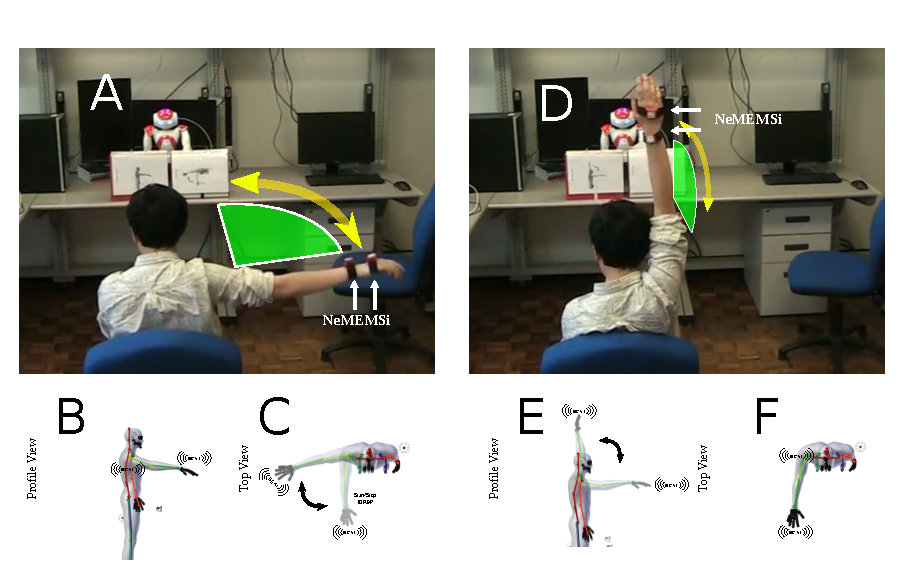
\includegraphics[width=1.0\textwidth]{hii}
    \caption
	[Human-image imitation (HII) activities]{
	{\bf Human-image imitation (HII) activities.} 
		(A) HII of horizontal arm movement, 
		(B) image of the profile view for horizontal arm movement,
		(C) image of the top view for horizontal arm movement,
		(D) HII of vertical arm movement, 
		(E) image of the profile view for vertical arm movement, and
		(F) image of the top view for horizontal arm movement.
		(B, C, F and E) show '(((BEAT)))' to indicate the participants
		arm movements synchronisation when hearing a sound beat.
        }
    \label{fig:hii}
\end{figure}
%%---------------------------------(FIGURE)------------------------------------
%%---------------------------------(FIGURE)-------------------------------------
\begin{figure}
  \centering
  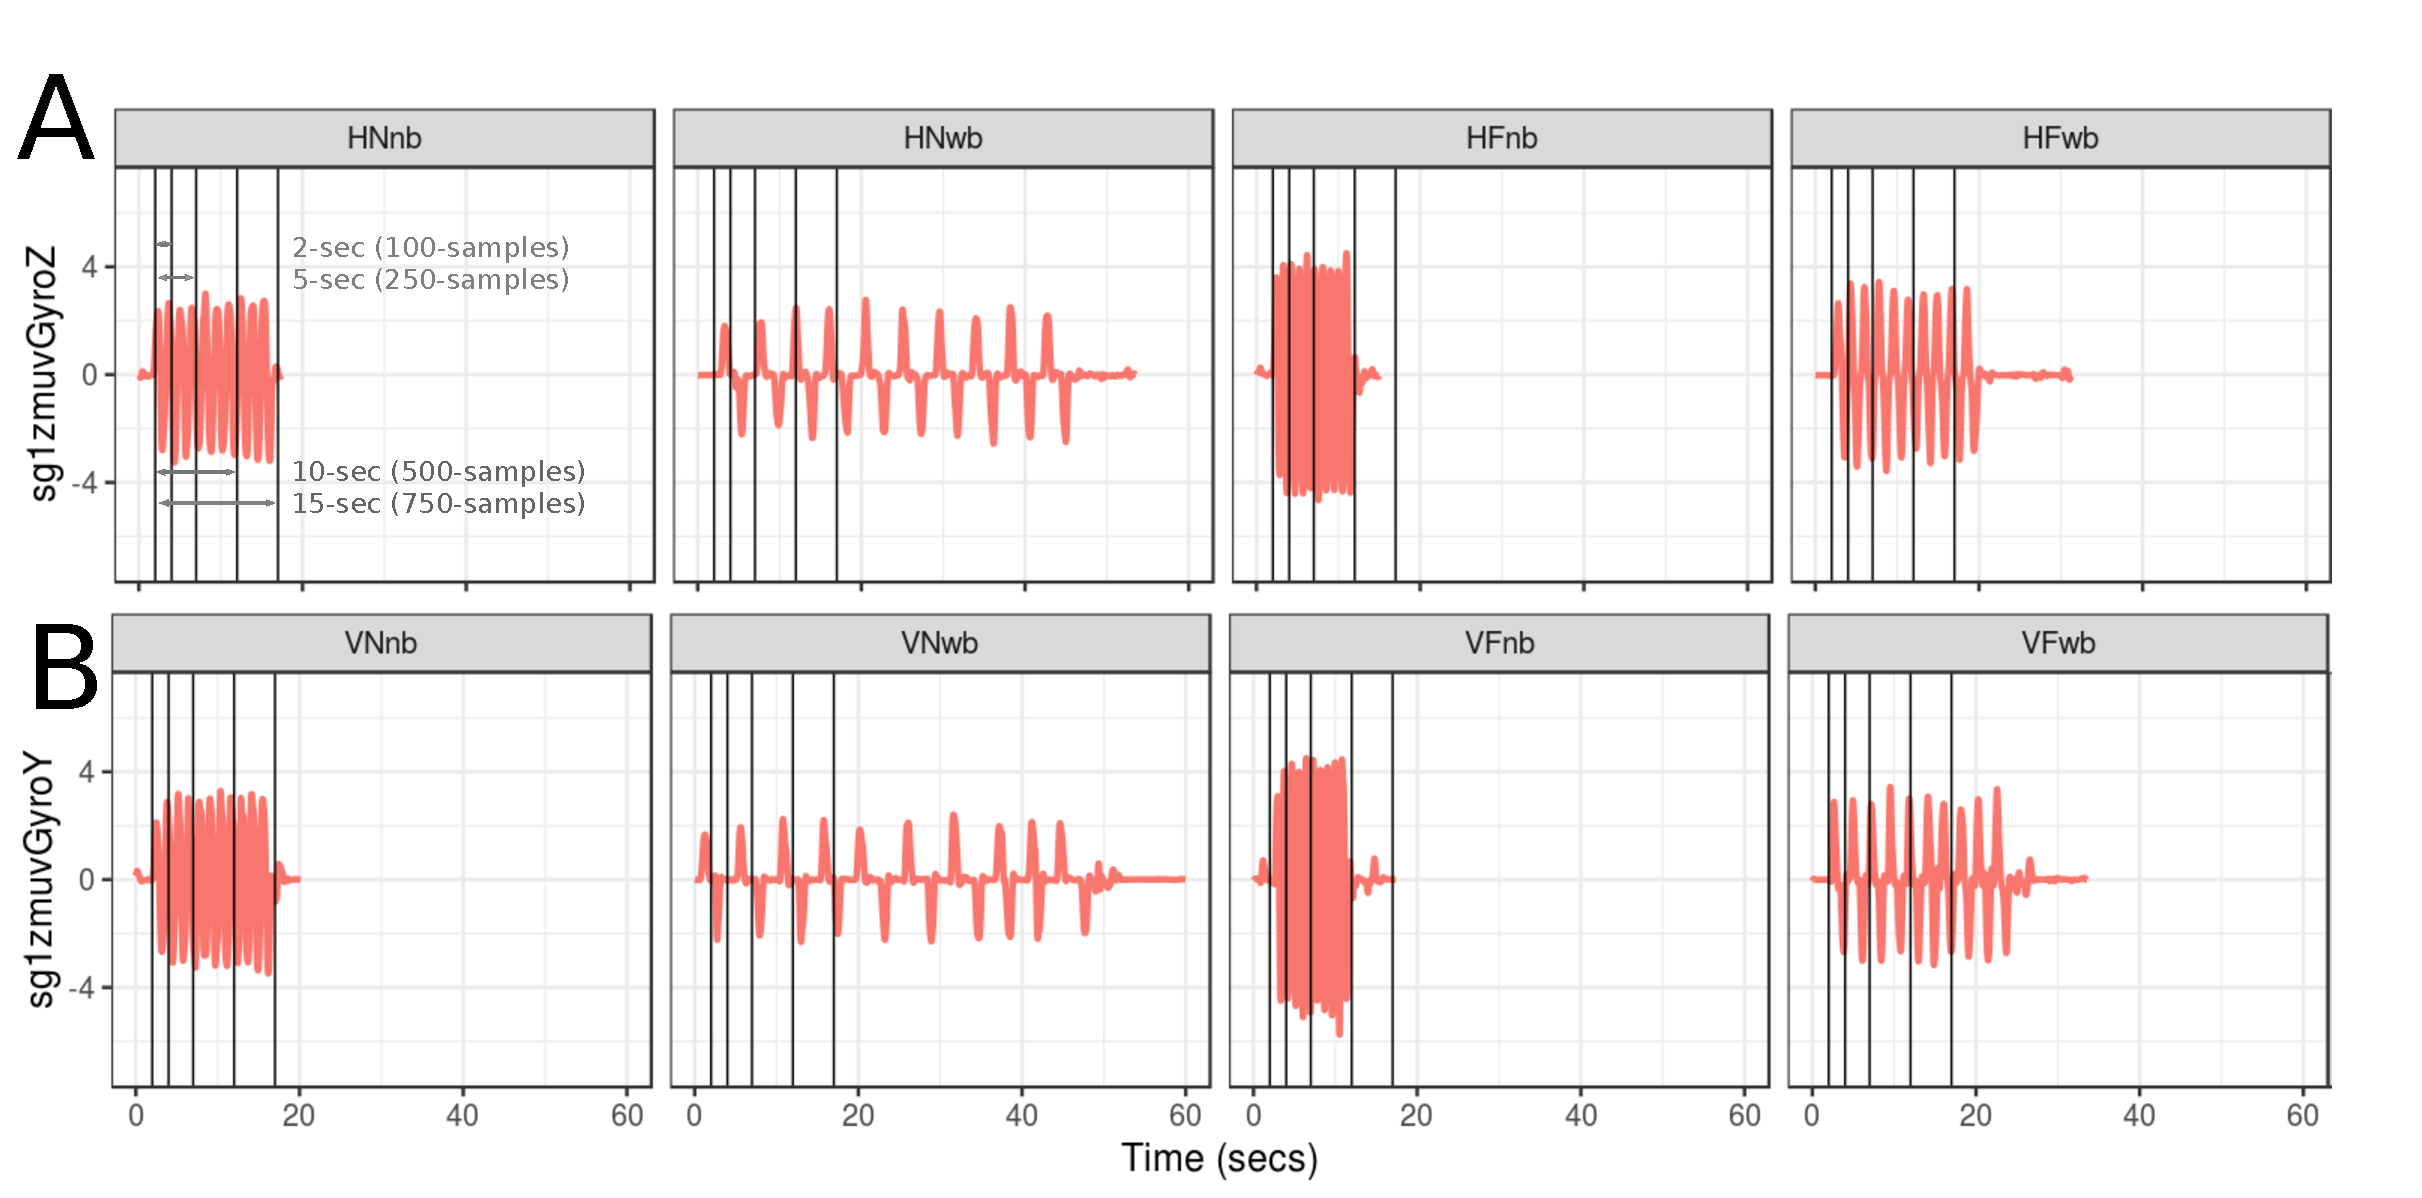
\includegraphics[width=1.0\textwidth]{fig_4_02}
    \caption
	[Time series for horizontal and vertical arm movements]{
	{\bf Time series for horizontal and vertical arm movements.} 
		Time series of smoothed data from gyroscope sensor 
		(sg1zmuvGyroZ and sg1zmuvGyroY) of participant 01 
		with sensor HS01 for different velocity arm movements: 
		(A) Horizontal Normal with no beat (HNnb),
			Horizontal Normal with beat (HNwb), 
			Horizontal Faster with no beat (HFnb) and
			Horizontal Faster with beat (HFwb), and 
		(B) Vertical Normal with no beat (HNnb),
			Vertical Normal with beat (HNwb), 
			Vertical Faster with no beat (HFnb) and
			Vertical Faster with beat (HFwb).
		Additionally, (A) presents vertical lines 
		to show window size lengths for 2-seconds 
		(100 samples), 5-seconds (250 samples), 
		10-seconds (500 samples) and 15-seconds (750 samples)
		which are presented in (B), (C) and (D).
	See Appendix \ref{appendix:d:ts} for 
	time series of all participants and activities. 
		R code to reproduce the figure is available \cite{hwum2018}.
        }
	\label{fig:hii-sts}
\end{figure}
%%---------------------------------(FIGURE)------------------------------------

\subsection{Human-humanoid imitation activities} \label{sec:experiment:hhi}
NAO is commonly used in human-robot interaction activities because 
its affordability, performance and modularity.
However, some of the limitations of NAO are related to 
(i) its 14 degrees of freedom (DOF) for arms and head,
(ii) the range of joint movement and 
(iii) joint torques and velocities \citep{gouaillier2009}. 
With that in mind, four NAO's arm movements 
that control the shoulder joint for vertical and horizontal
movements performed at normal and faster velocity 
were selected (Figs. \ref{fig:hri} B,D).
See Appendix \ref{appendix:nao} for basic and \cite{gouaillier2009}
for detailed information of NAO's mechanical and dynamic capabilities. 

For the human-humanoid imitation (HHI) experiment four wearable IMUs sensors 
were used in which two sensors were attached to the right hand of 
the participant and two sensors were attached to the left hand of 
the humanoid robot (Figure~\ref{fig:hri} A,C).
Then, in the face-to-face imitation activity, each participant was asked 
to imitate repetitions of simple horizontal and vertical arm movements 
performed by the humanoid robot in the following conditions:
\begin{itemize}[noitemsep,topsep=0pt]
\item ten repetitions of horizontal arm movement at normal (HN) and faster (HF) 
velocity (Fig.~\ref{fig:hri} A), and
\item ten repetitions of vertical arm movement at normal (VN) and faster (VF) 
velocity (Fig.~\ref{fig:hri} C).
\end{itemize}
%%---------------------------------(FIGURE)-------------------------------------
\begin{figure}
  \centering
  \includegraphics[width=1.0\textwidth]{hri}
    \caption
	[Human-humanoid imitation activities]{
	{\bf Human-humanoid imitation activities.} 
		Face-to-face human-humanoid imitation (HHI) activities for 
		(A) HHI of horizontal arm movement, 
		(B) Humanoid performing horizontal arm movement,
		(C) HHI of vertical arm movement, and 
		(D) Humanoid performing vertical arm movement.
        }
    \label{fig:hri}
\end{figure}
%%---------------------------------(FIGURE)------------------------------------

The duration of number of samples for NAO's arm movements were defined by 
normal and faster velocities of NAO's shoulder joint (Figs. \ref{fig:hri} B,D). 
Hence, the duration for one repetition of the horizontal 
arm movement at normal velocity, HN, is about 5 seconds considering that 
each repetition last around 250 samples. For horizontal arm movement at 
faster velocity, HF, each repetition were performed in around 2 seconds 
which correspond to 90 samples of data. 
The vertical arm movement at normal velocity, VN, were performed  in 6 seconds 
which is around 300 samples of data.
For vertical arm movement at faster velocity, VF, each repetition lasts 
about 2.4 seconds which correspond to 120 samples of data.
To visualise the distinction between normal and faster velocity for horizontal 
and vertical arm movements, Fig~\ref{fig:sts} shows smoothed time series 
for axes Z and Y of the gyroscope sensors with four window lengths: 
2-sec (100-samples), 5-sec (250-samples), 10-sec (500-samples) 
and 15-sec (750-samples).
See Appendix \ref{appendix:e:ts} for 
time series of all participants and activities. 
%%---------------------------------(FIGURE)-------------------------------------
\begin{figure}
  \centering
  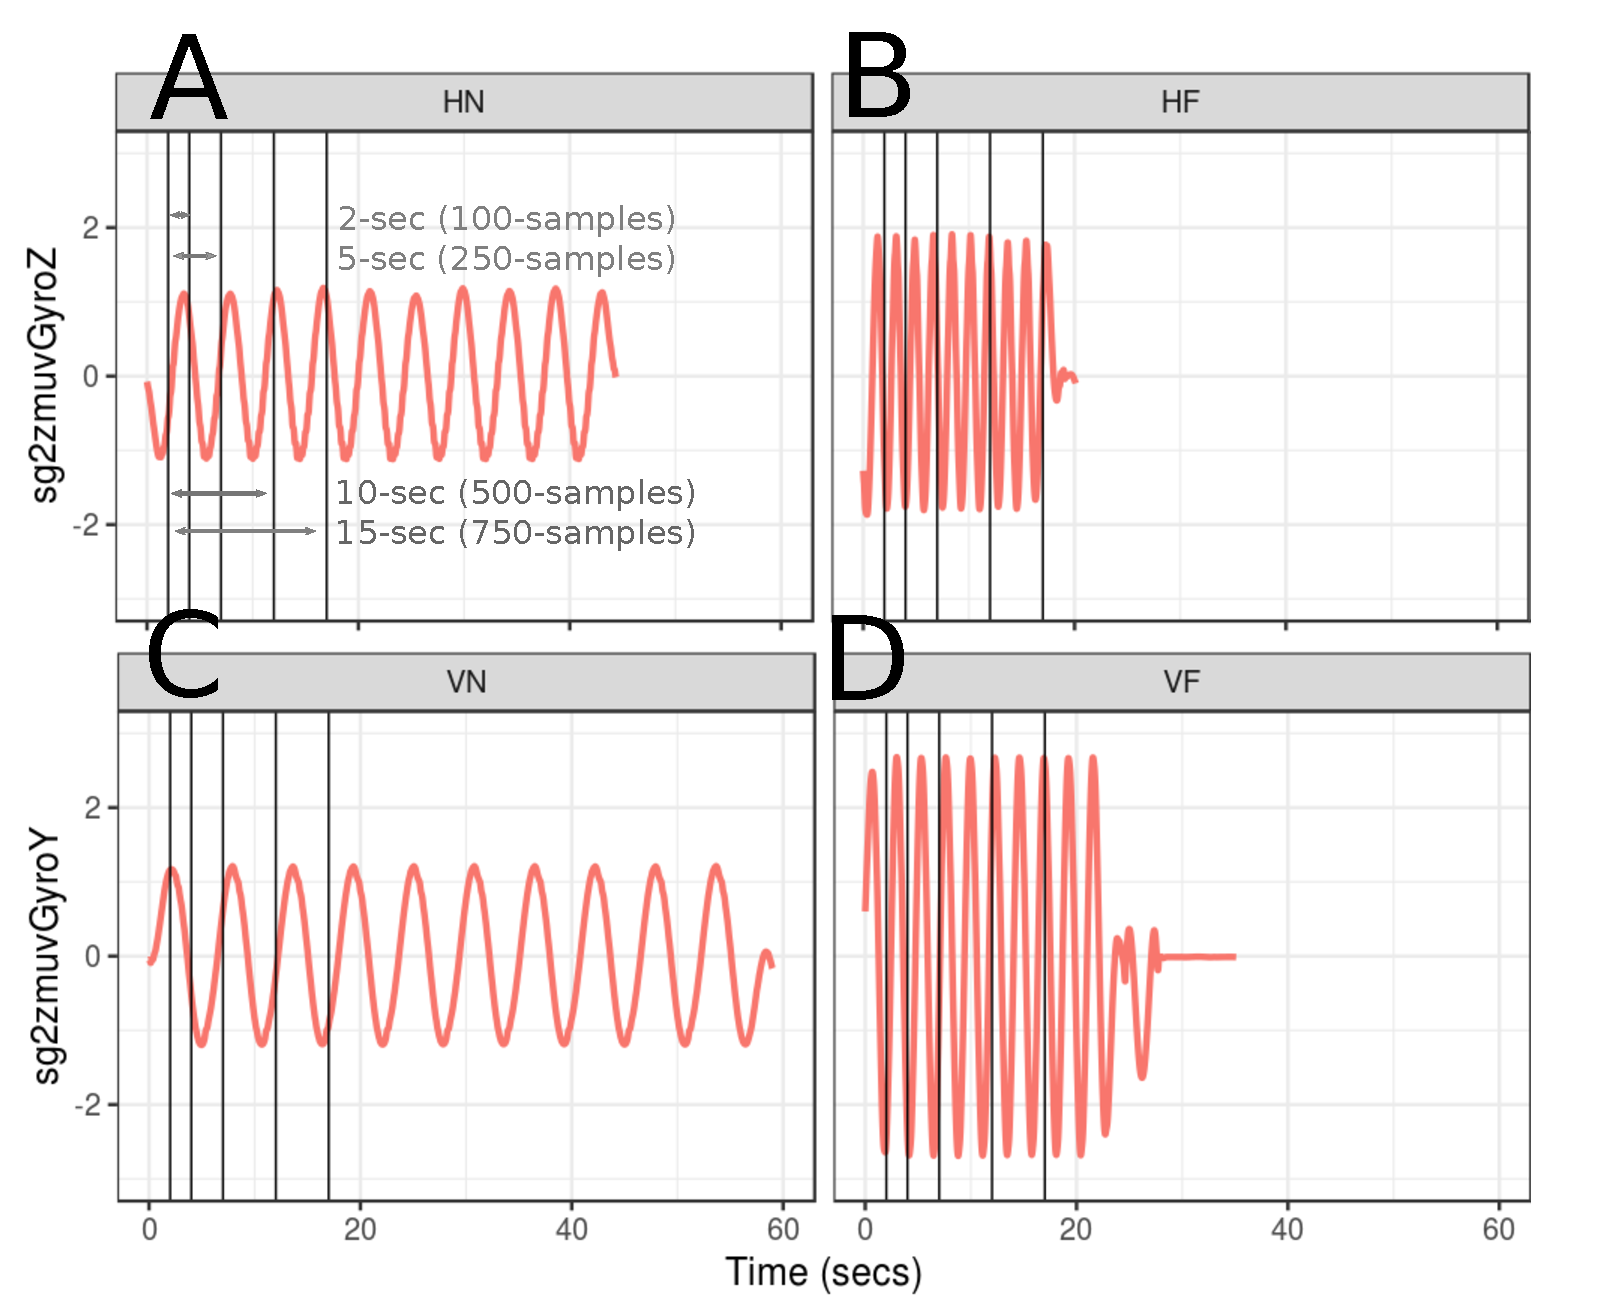
\includegraphics[width=1.0\textwidth]{fig_4_04}
    \caption
	[Time series duration of horizontal and vertical arm movements]{
	{\bf Time series duration of horizontal and vertical arm movements.} 
		Time series of smoothed data from gyroscope sensor 
		(sg1zmuvGyroZ and sg1zmuvGyroY) of NAO 
		with sensor HS01 for different velocity arm movements: 
		(A) Horizontal Normal arm movement, HN, 
		(B) Horizontal Faster arm movement, HF,
		(C) Vertical Normal arm movement, VN, and 
		(D) Vertical Faster arm movement, VF.
		Additionally, (A) presents vertical lines 
		to show window size lengths for 2-seconds 
		(100 samples), 5-seconds (250 samples), 
		10-seconds (500 samples) and 15-seconds (750 samples)
		which are presented in (B), (C) and (D).
		See Appendix \ref{appendix:e:ts} for 
		time series of all participants and activities. 
		R code to reproduce the figure is available \cite{hwum2018}.
        }
	\label{fig:sts}
\end{figure}
%%---------------------------------(FIGURE)------------------------------------

\section{Processing of time series} \label{sec:preparation_timeseries}

\subsection{Raw time-series}
For this thesis, analysis of time series is only with the accelerometer 
and gyroscope of the IMU sensors.
The justification for that is because \cite{shoaib2016} provided evidence 
of an improvement in recognition activities when only combining data 
from accelerometer and gyroscope. 
I also leave the magnetometer and quaternions time-series data for 
future investigations as these might create additional variations 
because of magnetic disturbances.

Time series from the accelerometer are defined by triaxial time series 
$A_x(n)$, $A_y(n)$, $A_z(n)$ which forms the matrix $\boldsymbol{A}$ 
(Eq.~\ref{eq:A}), and the same for data from the gyroscope which is 
defined by triaxial time-series of $G_x(n)$, $G_y(n)$, $G_z(n)$ representing 
the matrix $\boldsymbol{G}$ (Eq.~\ref{eq:G}). Both triaxial time series of 
each sensor, $a$ and $g$, are denoted with its respective axes 
subscripts $x,y,z$, where $n$ is the sample index and $N$ is the same 
maximum length of all axes for the time series.
Matrices $\boldsymbol{A}$ and $\boldsymbol{G}$ are represented as follow
%%---------------------------------(EQUATION)-----------------------------------
\begin{equation}\label{eq:A}
\boldsymbol{A} =
\begin{pmatrix}
  A_x(n) \\
  A_y(n) \\
  A_z(n)
\end{pmatrix}
=
\begin{pmatrix}
 a_x(1),a_x(2),\dots,a_x(N) \\
 a_y(1),a_y(2),\dots,a_y(N) \\
 a_z(1),a_z(2),\dots,a_z(N) 
\end{pmatrix},
\end{equation}
%%---------------------------------(EQUATION)-----------------------------------
%%---------------------------------(EQUATION)-----------------------------------
\begin{equation}\label{eq:G}
\boldsymbol{G} =
\begin{pmatrix}
 G_x(n) \\
 G_y(n) \\
 G_z(n)
\end{pmatrix}
=
\begin{pmatrix}
 g_x(1),g_x(2),\dots,g_x(N) \\
 g_y(1),g_y(2),\dots,g_y(N) \\
 g_z(1),g_z(2),\dots,g_z(N) 
\end{pmatrix},
\end{equation}
%%---------------------------------(EQUATION)-----------------------------------
where $n$ is the sample index and $N$ is the same maximum length of all axes 
for the time series.

\subsection{Postprocessing time-series}
After the collection of raw time-series from four NeMEMsi sensors,
time synchronisation alignment and interpolation were performed 
in order to create time series with same length and synchronised time.
See Appendix~\ref{appendix:b} for technical information 
about the IMU sensors and time synchronisation process.

\subsection{Window size of time-series}
With regard to the window size, \cite{shoaib2016} compared 
seven window lengths (2, 5, 10, 15, 20, 25, 30 seconds)
and tested a combination of inertial sensors (accelerometer, gyroscope and linear 
acceleration sensor) for activity recognition of repetitive 
activities (walking, jogging and biking) and less repetitive activities 
(smoking, eating, giving a talk or drinking a coffee).
\cite{shoaib2016} concluded that the increase of window size 
improved the recognition of complex activities (i.e. less repetitive 
activities which mainly involve random hand gestures).
With that in mind, four window sizes were selected 
for each of the activities, which are mainly repetitive, in this thesis: 
2-s window (100 samples), 
5-s window (250 samples), 
10-s (500 samples) and 
15-s window (750 samples).
Figures \ref{fig:hii-sts} and \ref{fig:sts} illustrate  
vertical lines to show four window size lengths which 
were chosen in order to cover a total time of 15 seconds (750 samples)
for either
(i) eight activities in human-image imitation 
or (ii) four activities in human-humanoid imitation.
Figures \ref{fig:hii-sts} and \ref{fig:sts} also show 
the starting point of time-series data from 2 seconds (100 samples) 
in order to avoid picking time-series data 
that do not correspond to the experiment 
(any movements before the experiment).
The latter statement is important for the application of methods
of nonlinear analysis as picking dynamics of time-series data 
that do not correspond to the activity
will therefore produce different results to the ones 
that only consider the duration of the activity. 

\subsection{Normalization of time-series}
Time series are normalised to have zero mean and unit variance 
using sample mean and sample standard deviation \citep{loffe2015}.
The sample mean and sample standard deviation using $x(n)$ is given by
%%---------------------------------(EQUATION)-----------------------------------
\begin{equation}\label{eq:ms}
\mu_{x(n)}= 
	\frac{1}{N} ( \sum_{i=1}^N x(i) ), \quad  
	\sigma_{x(n)} =  
	\sqrt{ \frac{  \sum_{1=1}^N ( x(i) - \mu_{x(n)} )^2 }{ N-1 }  },      
\end{equation}
%%---------------------------------(EQUATION)-----------------------------------
then the normalised data, $\hat{x}(n)$, is computed as follows
%%---------------------------------(EQUATION)-----------------------------------
\begin{equation}\label{eq:normalization}
\hat{x} (n) = \frac{   x(n) -  \mu_{x(n)}  }{   \sigma_{x(n)} }.   
\end{equation}
%%---------------------------------(EQUATION)-----------------------------------

%\newpage
\subsection{Smoothing time-series}
Applying low-pass filters is a common way to either capture low 
frequencies (below 15 Hz) that represent 99\% of the human body 
energy or to get the gravitational and body motion components of 
accelerations (below 0.3 Hz) \citep{anguita2013}.
However, filtering such information can cut-off frequencies that 
are important for the conservation of  
(i) the original properties of raw time-series data and 
(ii) the structure of the time-series data in terms of width and heights.
In addition to that, arm movements of NAO can sometimes produce 
jerky movements due to: 
(i) the control of dynamic response (fast acceleration/deceleration), 
(ii) the stiffness of the gear mechanism, or 
(iii) the high frequencies of oscillations because of resonances
(see Appendix \ref{appendix:nao} for NAO's mechanical and dynamic 
capabilities). 
Hence, instead of cutting out frequencies with a low-pass filter
for the experiments in the context of human-robot interaction, 
this thesis considers the application of Savitzky-Golay filter 
to smooth time series data in order 
to give insight into the effect of smoothness of real-world 
time series data with methods of nonlinear analysis.

Savitzky-Golay filter is based on the principle of moving 
window average which preserves the area under the curve (the zeroth moment)
and its mean position in time (the first moment) but the line width 
(the second moment) is violated and that results, for example, in the case 
of spectrometric data where a narrow spectral line is presented with 
reduced height and width \citep{press1992}.
The aim of Savitzky-Golay filtering is hence to find the filter coefficients 
$c_n$ that preserve higher momentums which are based on local least-square 
polynomial approximations 
\citep{savitzkygolay1964, press1992, schafer2011}.
Therefore, Savitzky-Golay coefficients are computed using an R function 
\texttt{sgolay(p,n,m)} where \texttt{p} is the filter order, 
\texttt{n} is the filter length (must be odd) 
and \texttt{m} is the $m$-th derivative of the filter coefficients 
\citep{Rsignal}. Smoothed signal is represented with a tilde over the 
original signal: $\tilde{x}(n)$.

 %Experiments

%%*******************************************************************************
%****************************** Fifth Chapter **********************************
%*******************************************************************************

\chapter{Quantifying Human-Image Imitation Activities} \label{chapter5}

%% **************************** Define Graphics Path **************************
%\ifpdf
%    \graphicspath{{chapter5/figs/raster/}{chapter5/figs/PDF/}{chapter5/figs/}}
%\else
%    \graphicspath{{chapter5/figs/vector/}{chapter5/figs/}}
%\fi
%

\graphicspath{{figs/chapter5/PDF/}}

\section{Introduction}
In this chapter, results for experiments of human-image imitation 
activities, described in Section \ref{sec:experiment:hii},  
are presented by including time series, minimum embedding parameters, 
the reconstructed state spaces (RSS) using 
uniform time-delay embedding technique (UTDE), 
recurrence plots (RP),
recurrent quantification analysis (RQA), and 
weaknesses and strengthens of RQA with 
three dimensional surface plots of RQA. 

Time series data for this experiment are described as follows:
\begin{itemize}

\item Six participants defined as $pN$ where $N$ is the number of 
	participant.

\item Three levels of smoothness for the normalised data 
(sg0zmuv, sg1zmuv and sg2zmuv), computed from two different filter 
lengths (29 and 159) with the same polynomial degree of 5 using the 
function \texttt{sgolay(p,n,m)} \citep{Rsignal},

\item Four window lengths: 2-sec (100 samples), 5-sec (250 samples), 
	10-sec (500 samples) and 15-sec (750 samples), and 

\item Eight velocities of arm movement activity: 
horizontal movements in normal and faster velocity with no
beat (HNnb, HFnb) and with beat (HNwb, HFwb), 
and 
vertical movements in normal and faster velocity with no
beat (VNnb, VFnb) and with beat (VNwb, VFwb).

\end{itemize}
To make the visual comparison easier, time series for only 
three participants ($p04$, $p05$, $p10$) with a window length 
of 10 seconds are considered for the following results.
See Appendix \ref{appendix:e} for further results.

%\newpage
\section{Time series}
Figures \ref{fig:tsH-hii} and \ref{fig:tsV-hii} show time series for 
horizontal and vertical arm movements of participants 
following an image while not hearing a beat (nb) and hearing a beat (wb).
Also, three levels of smoothness of normalised time series are presented
 (sg0, sg1 and sg2).
The remaining time series are presented in Appendix \ref{appendix:e:ts}.
%%---------------------------------(FIGURE)-------------------------------------
\begin{figure}
\centering
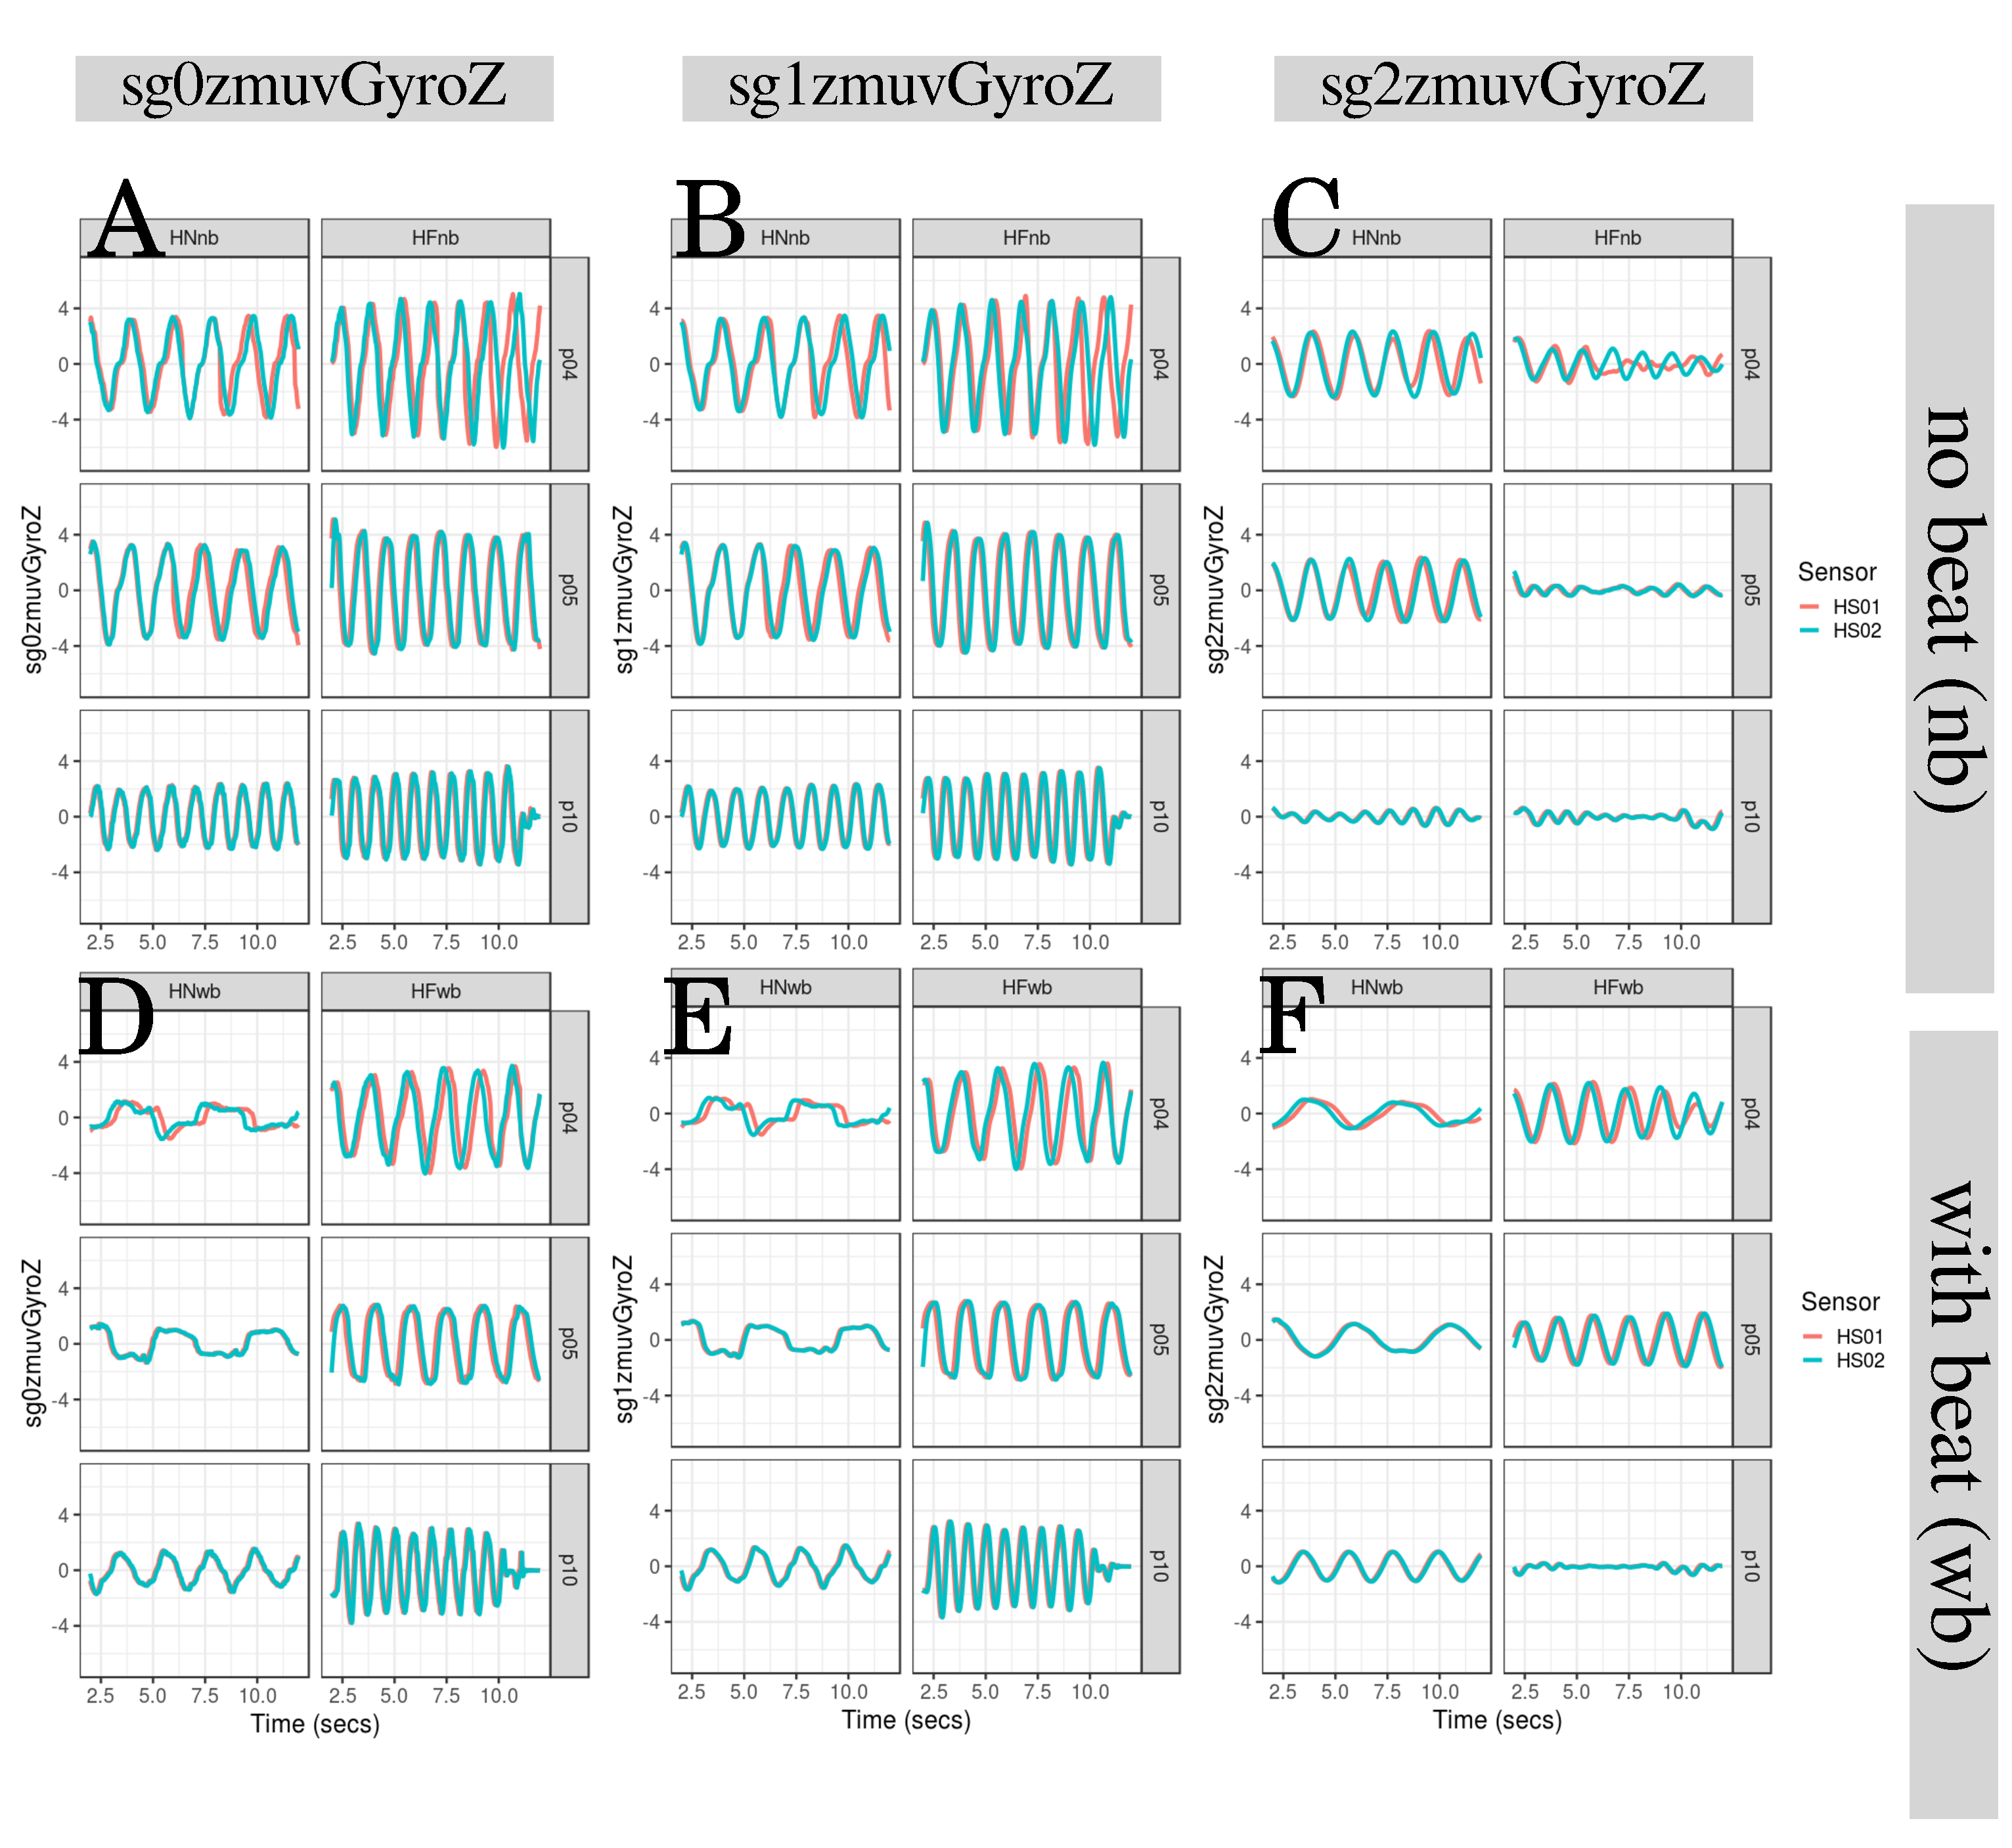
\includegraphics[width=0.99\textwidth]{fig_5_01}
    	\caption
	[Time series for horizontal arm movements]{
	{\bf Time series for horizontal arm movements.}
		Time series for (A,D) raw-normalised (sg0zmuvGyroZ), 
		(B,E) normalised-smoothed 1 (sg1zmuvGyroZ), and
		(C,F) normalised-smoothed 2 (sg2zmuvGyroZ).
		Time series are for three participants 
		($p04$, $p05$, and $p10$) 
		for horizontal movements in normal and faster velocity with
		no beat	(HNnb, HFnb) and with beat (HNwb, HFwb) using 
		the normalised GyroZ axis (zmuvGyroZ) and 
		two sensors attached to the participant wrist (HS01, HS02).
	\R code to reproduce the figure is available at 
	\codelink{https://github.com/mxochicale-phd/thesis/tree/master/0_code_data/1_code/7_figs_ch5/01_fig5.1-5.2}.
        }
    \label{fig:tsH-hii}
\end{figure}
%%---------------------------------(FIGURE)-----------------------------------
%%---------------------------------(FIGURE)-------------------------------------
\begin{figure}
\centering
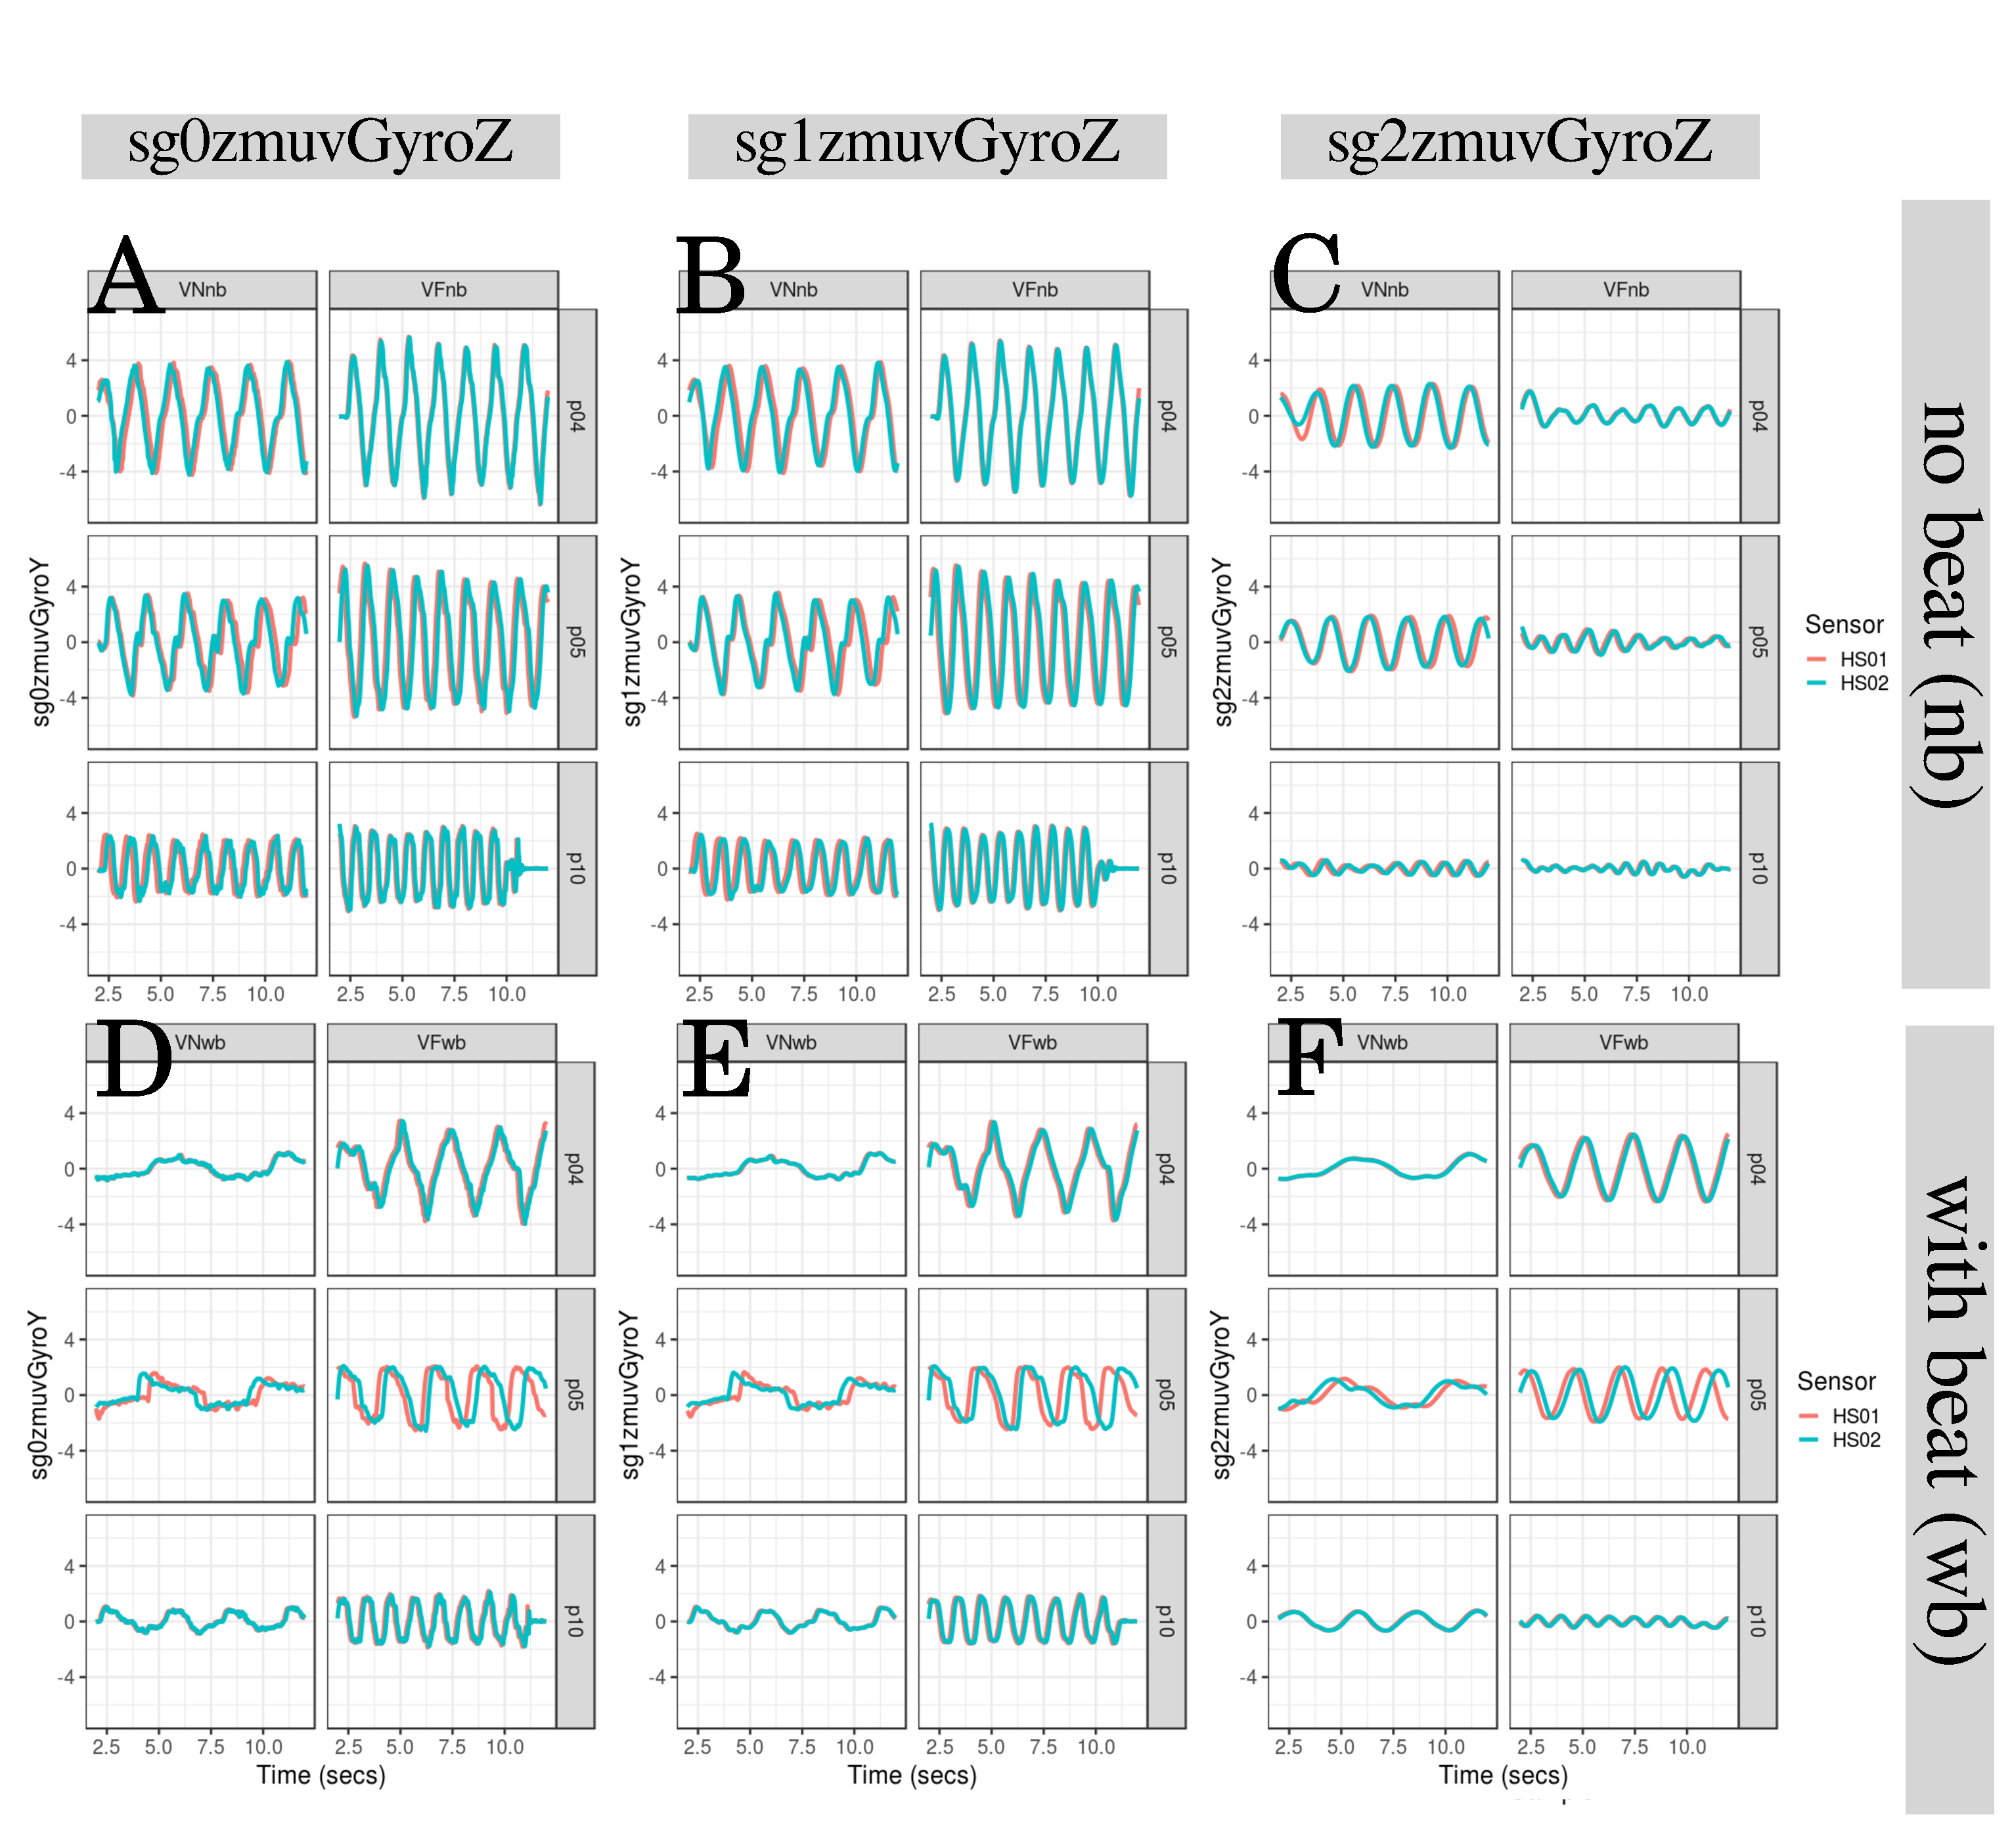
\includegraphics[width=0.99\textwidth]{fig_5_02}
    	\caption
	[Time series for vertical arm movements]{
	{\bf Time series for vertical arm movements.}
		Time series for (A,D) raw-normalised (sg0zmuvGyroY), 
		(B,E) normalised-smoothed 1 (sg1zmuvGyroY), and
		(C,F) normalised-smoothed 2 (sg2zmuvGyroY).
		Time series are for three participants 
		($p04$, $p05$, and $p10$) 
		for vertical movements in normal and faster velocity with
		no beat	(VNnb, VFnb) and with beat (VNwb, VFwb) using the 
		normalised GyroY axis (zmuvGyroY) and two sensors 
		attached to the participant wrist (HS01, HS02).
	\R code to reproduce the figure is available at 
	\codelink{https://github.com/mxochicale-phd/thesis/tree/master/0_code_data/1_code/7_figs_ch5/01_fig5.1-5.2}.
        }
    \label{fig:tsV-hii}
\end{figure}
%%---------------------------------(FIGURE)------------------------------------

\newpage
\section{Minimum Embedding Parameters} \label{mep-hii}
The first step to create Reconstructed State Spaces (RSSs) with the use of
Uniform Time-Delay Embedding (UTDE) is to compute the
average minimum embedding parameters for all participants, sensors and 
activities using False Nearest Neighbour (FNN) and 
Average Mutual Information (AMI) algorithms.

%\subsection{Minimum dimension embedding values}
Hence, Figs. \ref{fig:CAO-hii} illustrate the box plots for minimum 
embedding dimensions.
For horizontal arm movements (Figs. \ref{fig:CAO-hii}(A)), 
one can notice how the interquartile range  
appear to be near to one independently of the 
activity or sensor. 
With regards to the level of smoothness,
there is a decrease of sample mean (gray rhombus) 
as the smoothness increase.  
Similarly, for vertical arm movements (Figs. \ref{fig:CAO-hii}(B))
the interquartile range of activities and sensors 
appears to be near to one. In addition to that, 
the increase of smoothness is affected by a decrease 
in sample means (gray rhombus) meaning that there is 
a decrease of dimensionality of the dynamics of 
the time series data.
For further details of the minimum dimension values see
Figures in Appendix \ref{appendix:e:ep}.
%%---------------------------------(FIGURE)-------------------------------------
\begin{figure}
\centering
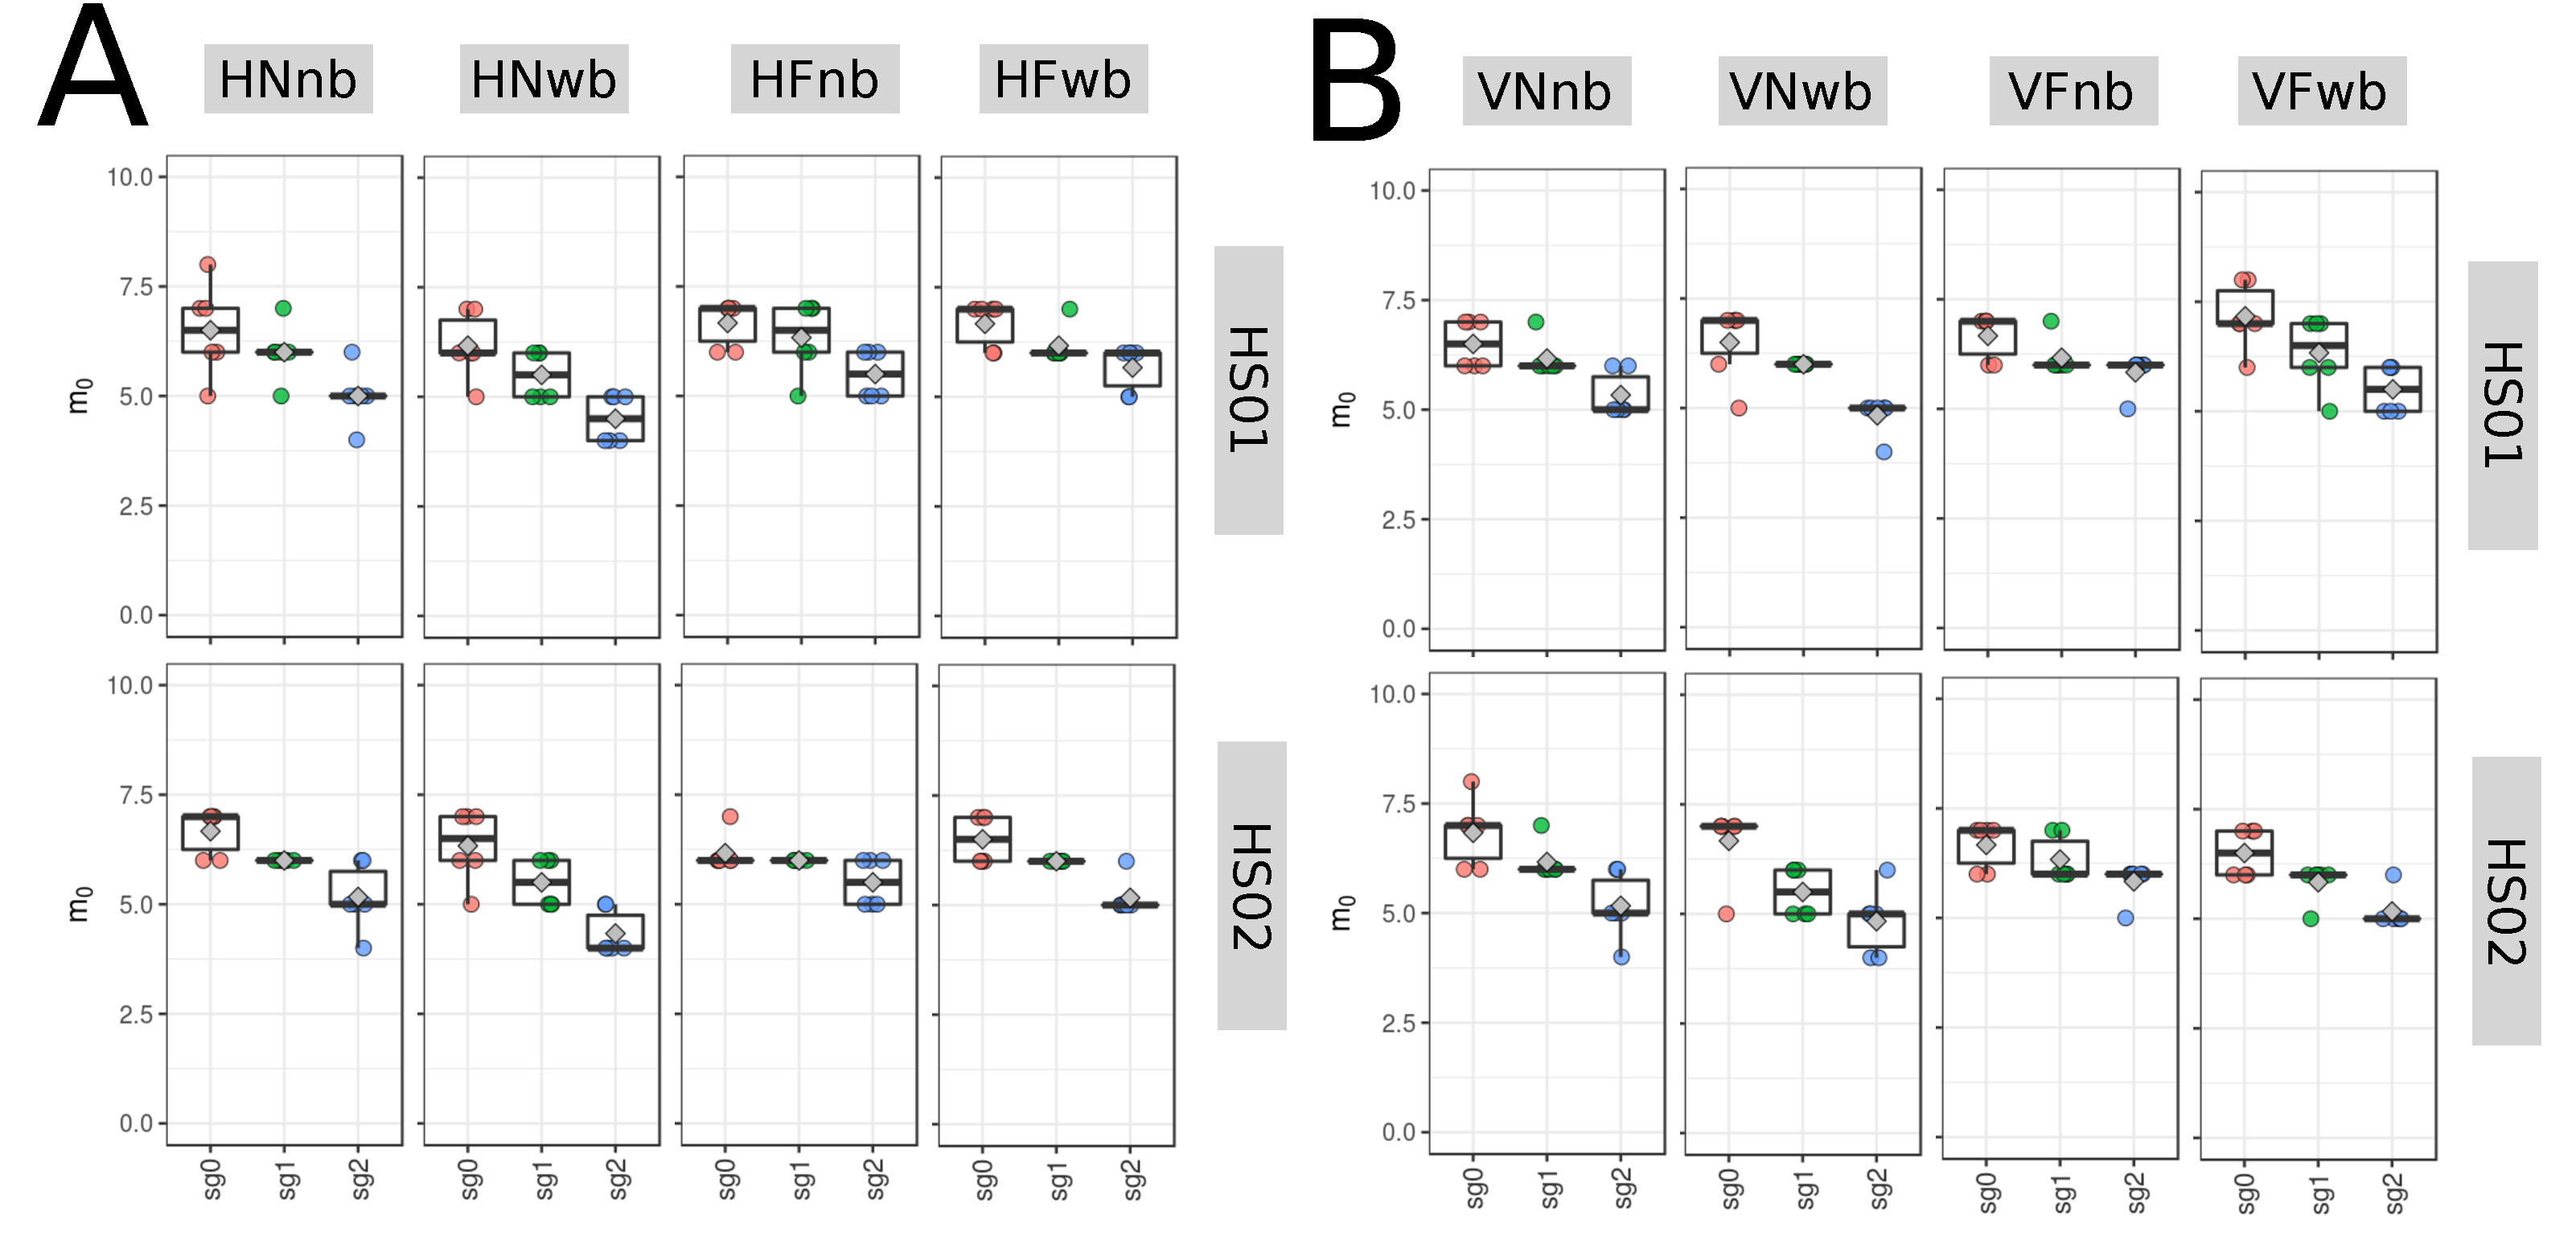
\includegraphics[width=0.95\textwidth]{fig_5_03}
	\caption
	[Box plots for minimum embedding dimensions]{
	{\bf Box plots for minimum embedding dimensions.} 
		Box plots of minimum embedding dimensions for 
		(A) horizontal and (B) vertical arm movements for
		normal  and faster velocity (N/F) with no beat (nb) 
		and with beat (wb) movements
		using sensors 01 and 02 attached to the wrist of the 
		participant (HS01, HS02).
		Minimum embedding dimensions are for six participants 
		($p01$, $p04$, $p05$, $p10$, $p11$, $p15$) with three 
		smoothed signals (sg0, sg1 and sg2)
		and window length of 10 seconds.
	\R code to reproduce the figure is available at 
	\codelink{
	https://github.com/mxochicale-phd/thesis/tree/master/0_code_data/1_code/7_figs_ch5/02_fig5.3/code
	}.
        }
    \label{fig:CAO-hii}
\end{figure}
%%---------------------------------(FIGURE)-------------------------------------

%\subsection{Minimum delay embedding values}
Figs. \ref{fig:AMI-hii} illustrate the box plots for first minimum AMI.
Box plots for horizontal arm movements (Figs. \ref{fig:AMI-hii}(A)) for 
HNwb appear more spread (interquartile range between 10 to 20) while 
other activities there is a slight variation of values 
(interquartile range between 5 to 10).
Little can be said regardless the sample mean of each axis (gray rhombus) 
which is not proportionally affected as the smoothed of the time series 
increase.
Box plots for vertical arm movements (Figs. \ref{fig:AMI-hii}(B)) 
show that the interquartile range of each activity is constant
except for the activity VFwb.
Additionally, the increase of smoothness of time series (sg0 to sg2) made 
the sample mean (gray rhombus) to increase which means that 
the maximal information to knowledge from $x(n)$ to $x(t+\tau_0)$ also 
increase.
For further details of the minimum dimension values see
Figures in Appendix \ref{appendix:e:ep}.
%%---------------------------------(FIGURE)-------------------------------------
\begin{figure}
\centering
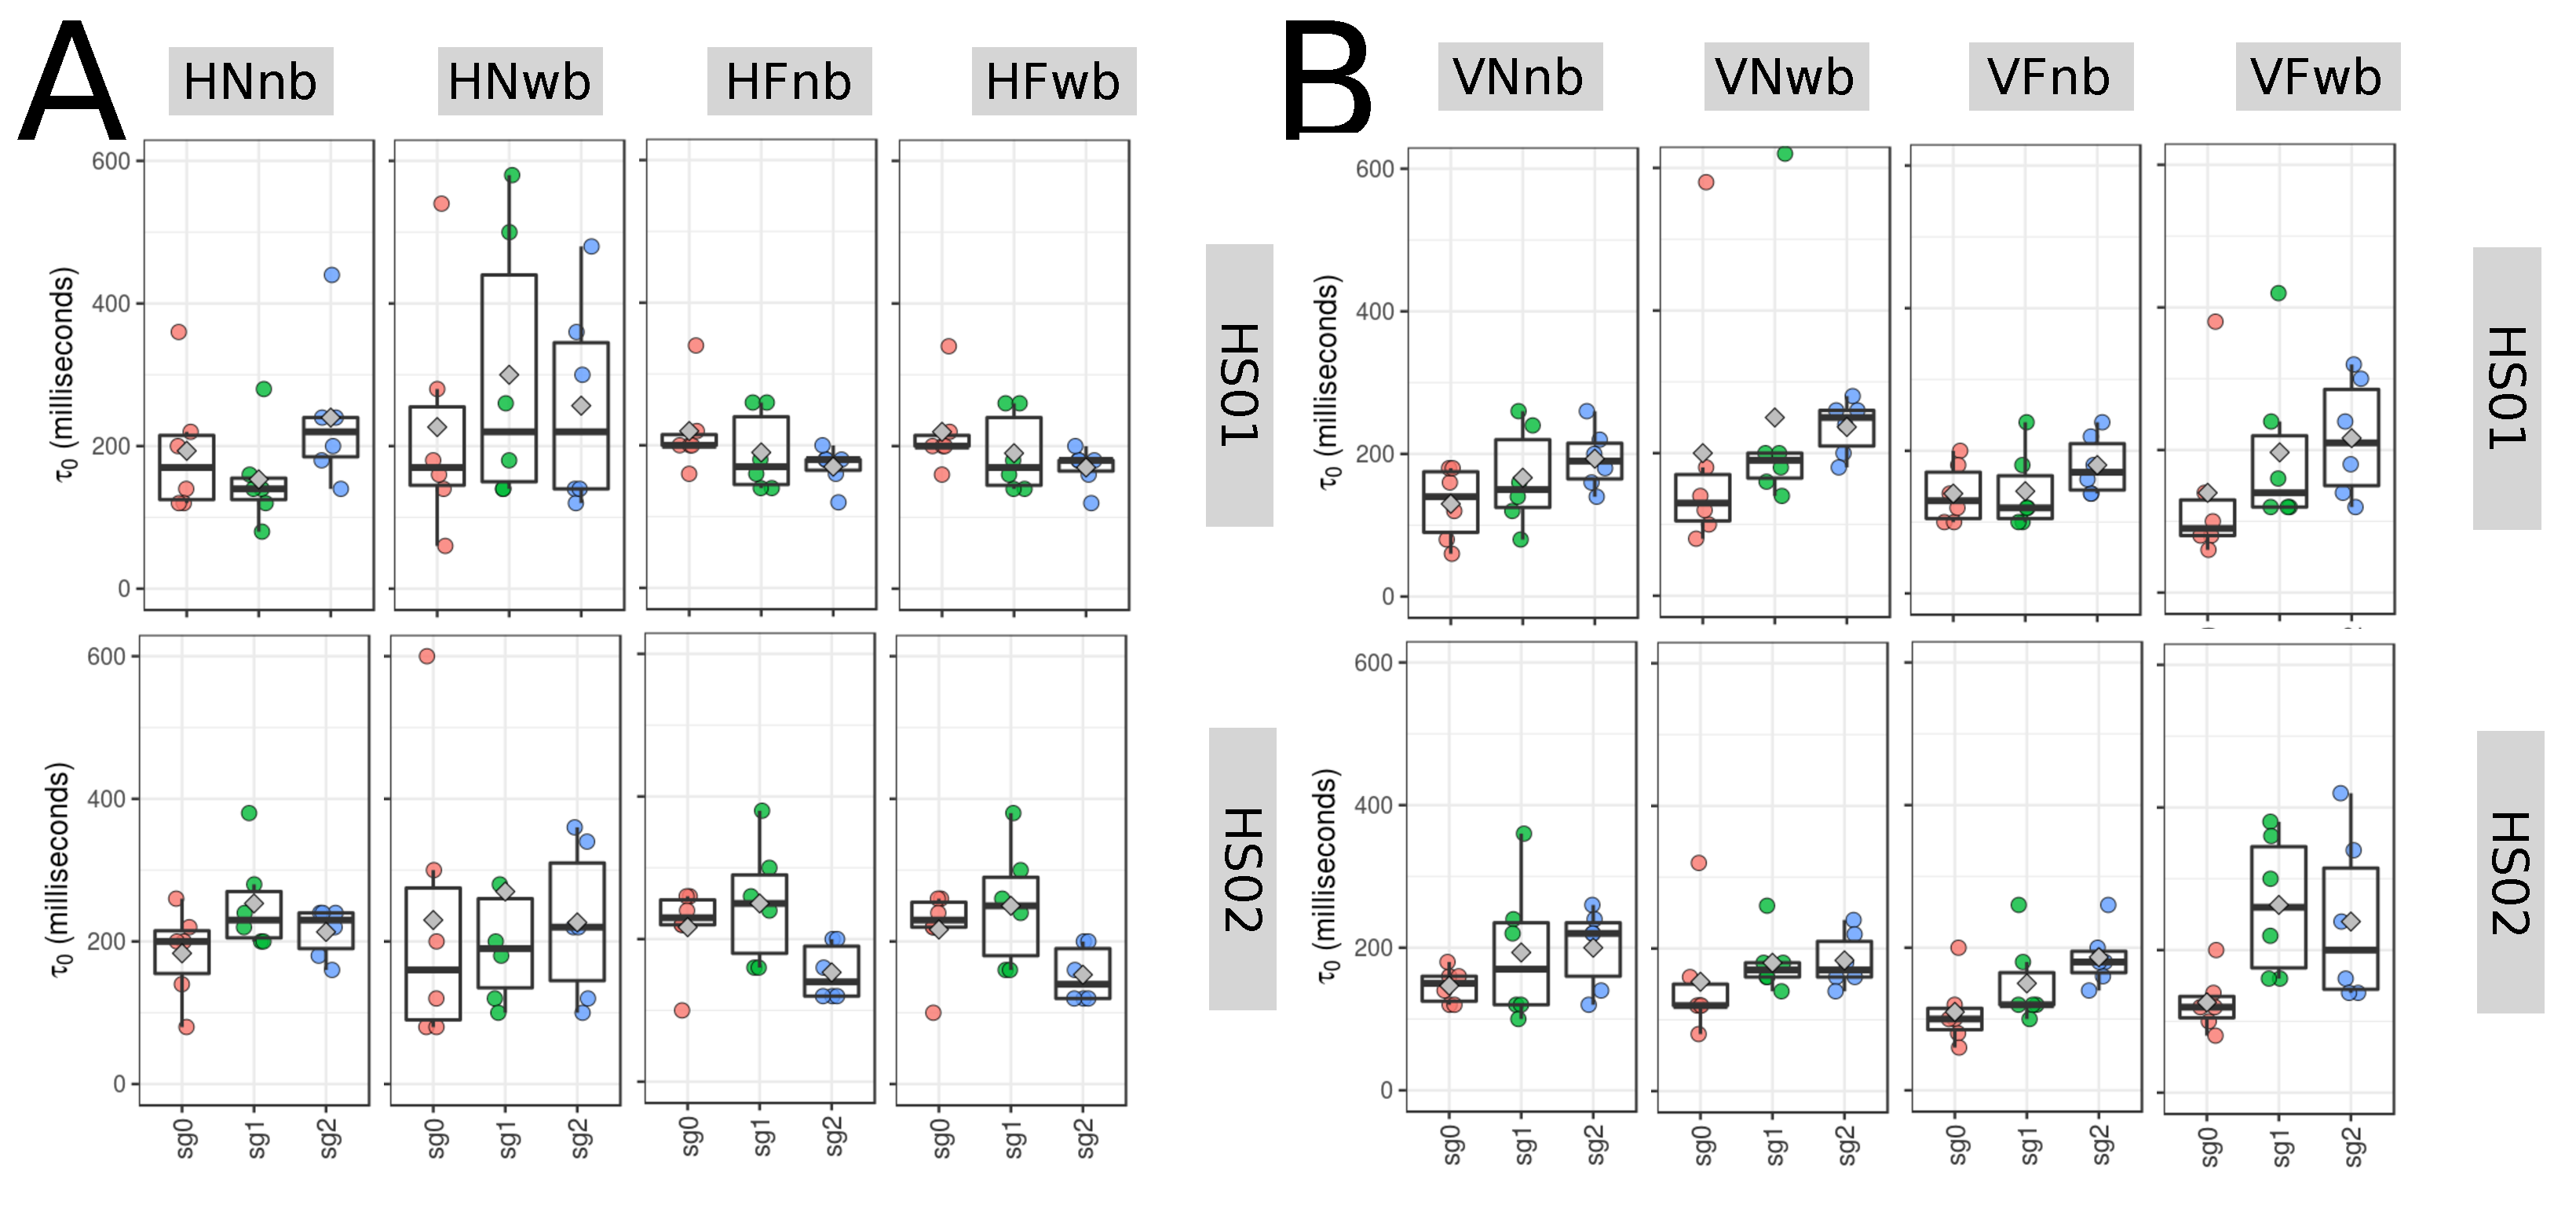
\includegraphics[width=0.95\textwidth]{fig_5_04}
	\caption
	[Box plots for 1st minimum AMI]{
	{\bf Box plots for 1st minimum AMI.} 
		Box plots of the 1st minimum AMI values for 
		(A) horizontal and (B) vertical arm movements for
		normal and faster velocity (N/F) with no beat (nb) 
		and with beat (wb) movements
		using sensors 01 and 02 attached to the wrist of the 
		participant (HS01, HS02).
		First minimum AMI values in milliseconds are 
		for six participants 
		($p01$, $p04$, $p05$, $p10$, $p11$, $p15$) with three 
		smoothed signals (sg0, sg1 and sg2)
		and window length of 10 seconds.
	\R code to reproduce the figure is available at 
	\codelink{
	https://github.com/mxochicale-phd/thesis/tree/master/0_code_data/1_code/7_figs_ch5/03_fig5.4/code
	}.
        }
    \label{fig:AMI-hii}
\end{figure}
%%---------------------------------(FIGURE)-------------------------------------

\newpage
\subsection{Average minimum embedding parameters}
Although the implementation of Uniform Time-Delay Embedding (UTDE) 
is simple, the main challenge is the selection of appropriate embedding 
parameters to reconstruct the state spaces of each time series
as these are unique in terms of its structure (modulation of amplitude, 
frequency and phase) \citep{ frank2010, sama2013, bradley2015}.
With that in mind, one problem that this thesis has faced 
is the selection of embedded parameters that 
can represent all time series. 
The solution to that problem was to compute a sample mean over 
all values for all participants, activities and sensors
(Section \ref{sec:overall_minMT}).
Hence, the average minimum embedding parameters is computed with 
a sample mean of $\overline{m}_0=6$ from the minimum values 
of $E_{1}(m)$ in Figs \ref{fig:CAO-hii} and a sample mean 
of $\overline{\tau}_0=10$ from minimum values of AMIs in Figs \ref{fig:AMI-hii}.
Hence, Reconstructed State Spaces (RSSs), Recurrence Plots (RPs) and
Recurrence Quantification Analysis (RQA) metrics
are computed with the average minimum embedding parameters 
($\overline{m_0}=6$, $\overline{\tau_0}=10$).

\section{Reconstructed state spaces with UTDE}
Reconstructed state spaces for horizontal normal and horizontal faster 
arm movements with no beat are shown in Fig \ref{fig:rss_Hnb_w500}.
The smoothness of the time series show a slightly change of smoothed 
trajectories in the RSSs for sg0zmuvGyroZ and sg1zmuvGyroZ, while the 
RSSs trajectories for sg2zmuvGyroZ appear to be distorted 
(Fig \ref{fig:rss_Hnb_w500}).
One can see slightly differences in the RSSs trajectories when comparing 
sensors HS01 and HS02 for horizontal normal arm movement with no beat 
(Fig \ref{fig:rss_Hnb_w500}(A, B)) and horizontal faster arm movements 
with no beat (Fig \ref{fig:rss_Hnb_w500}(C, D)).
With regards to the type of movement, the RSSs trajectories appear 
to change little when comparing horizontal normal with faster arm movements 
(Fig \ref{fig:rss_Hnb_w500}).

Fig \ref{fig:rss_Hwb_w500} shows trajectories of the reconstructed 
state space for horizontal normal and horizontal faster arm movements 
while beat sounds. Hence, as in Fig \ref{fig:rss_Hnb_w500}, 
it can also be noted in Fig \ref{fig:rss_Hwb_w500} that the smoothness 
of sg0zmuvGyroZ and sg1zmuvGyroZ appear to affect little the RSSs 
trajectories, while RSSs trajectories for sg2zmuvGyroZ substantially change 
so as to show different patterns. However, the trajectories in the RSS 
appear to change little when comparing the differences between the type 
of sensors HS01 and HS02 (Fig \ref{fig:rss_Hwb_w500}).
For the type of movements, trajectories show differences for horizontal
normal and horizontal faster arm movements (Fig \ref{fig:rss_Hwb_w500}).

Fig \ref{fig:rss_Vnb_w500} show trajectories for reconstructed state spaces
of vertical normal and vertical faster arm movements with no beat. 
Smoothness of the RSSs trajectories is slightly noticed for sg0zmuvGyroY and
sg1zmuvGyroY, whereas RSSs trajectories for sg2zmuvGyroY are evidently 
different (Fig \ref{fig:rss_Vnb_w500}).
When comparing the RSSs trajectories from sensors HS01 and HS02,
it can be noted little change, whereas the comparison from type of movement, 
the trajectories difference is more notable (Fig \ref{fig:rss_Vnb_w500}).

Fig \ref{fig:rss_Vwb_w500} show trajectories for reconstructed state space
of vertical normal and vertical faster arm movements for participants 
hearing a beat. Smoothness of RSSs trajectories appear to show slightly 
differences between sg0zmuvGyroY and sg1zmuvGyroY, however RSSs trajectories 
for sg2zmuvGyroY are different (Fig \ref{fig:rss_Vwb_w500}).
With regards to the type of sensor HS01 and HS02, RSSs trajectories appear 
to change little, whereas for type of activity of normal and faster arm 
movements, RSSs trajectories show evidently differences 
(Fig \ref{fig:rss_Vwb_w500}).

%%---------------------------------(FIGURE)-------------------------------------
\begin{figure}
\centering
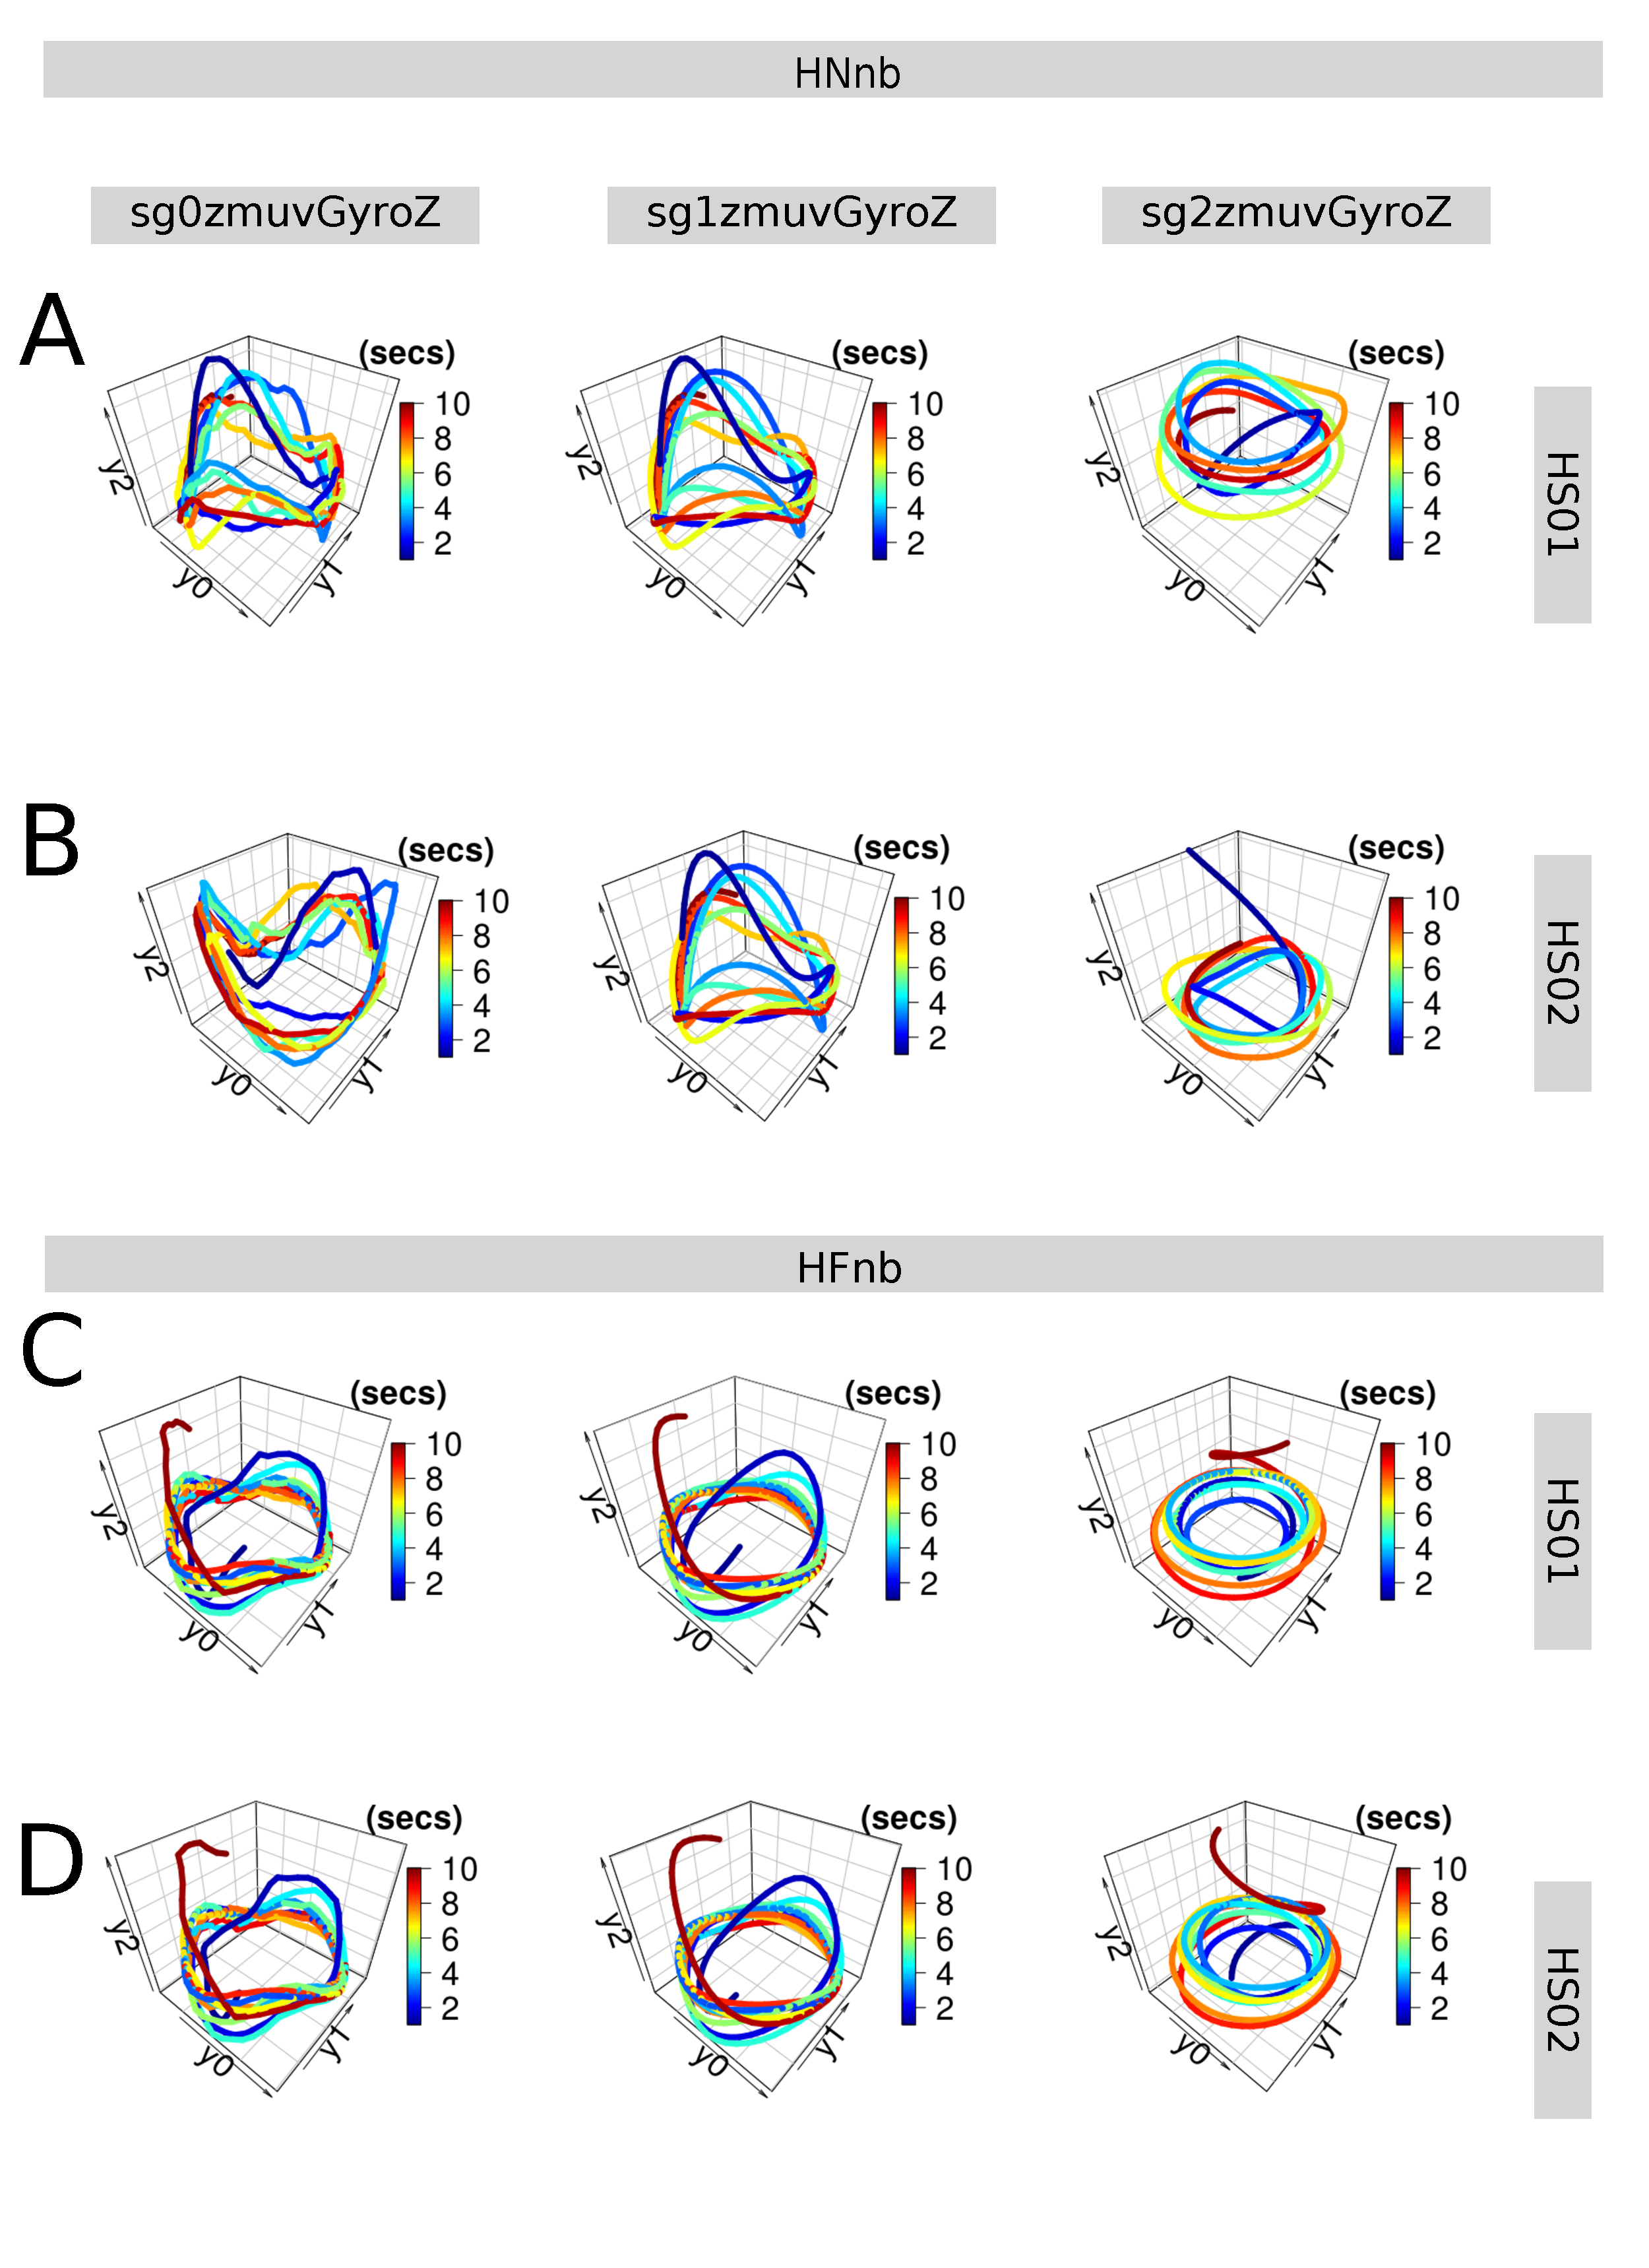
\includegraphics[height=0.8\textheight]{fig_5_05}
\caption
	[RSSs for horizontal arm movements (no beat)]{
	{\bf RSSs for horizontal arm movements (no beat).}
	Reconstructed state spaces of participant p01 for 
	(A, B) horizontal normal movements with no beat (HNnb) and 
	(C, D) horizontal faster velocity with no beat (HFnb).
	Time series for raw-normalised (sg0zmuvGyroZ), 
	normalised-smoothed 1 (sg1zmuvGyroZ) and 
	normalised-smoothed 2 (sg2zmuvGyroZ) with
	(A, C) sensor attached to the participant (HS01), and
	(B, D) sensor attached to the participant (HS02).	
	Reconstructed state spaces were computed with 
	embedding parameters $\overline{m_0}=6$, $\overline{\tau_0}=10$.
	\R code to reproduce the figure is available at 
	\codelink{
	https://github.com/mxochicale-phd/thesis/tree/master/0_code_data/1_code/7_figs_ch5/04_fig5.5-5.6-5.7-5.8/code
	}.
        }
     \label{fig:rss_Hnb_w500}
\end{figure}
%%---------------------------------(FIGURE)------------------------------------

%%---------------------------------(FIGURE)-------------------------------------
\begin{figure}
\centering
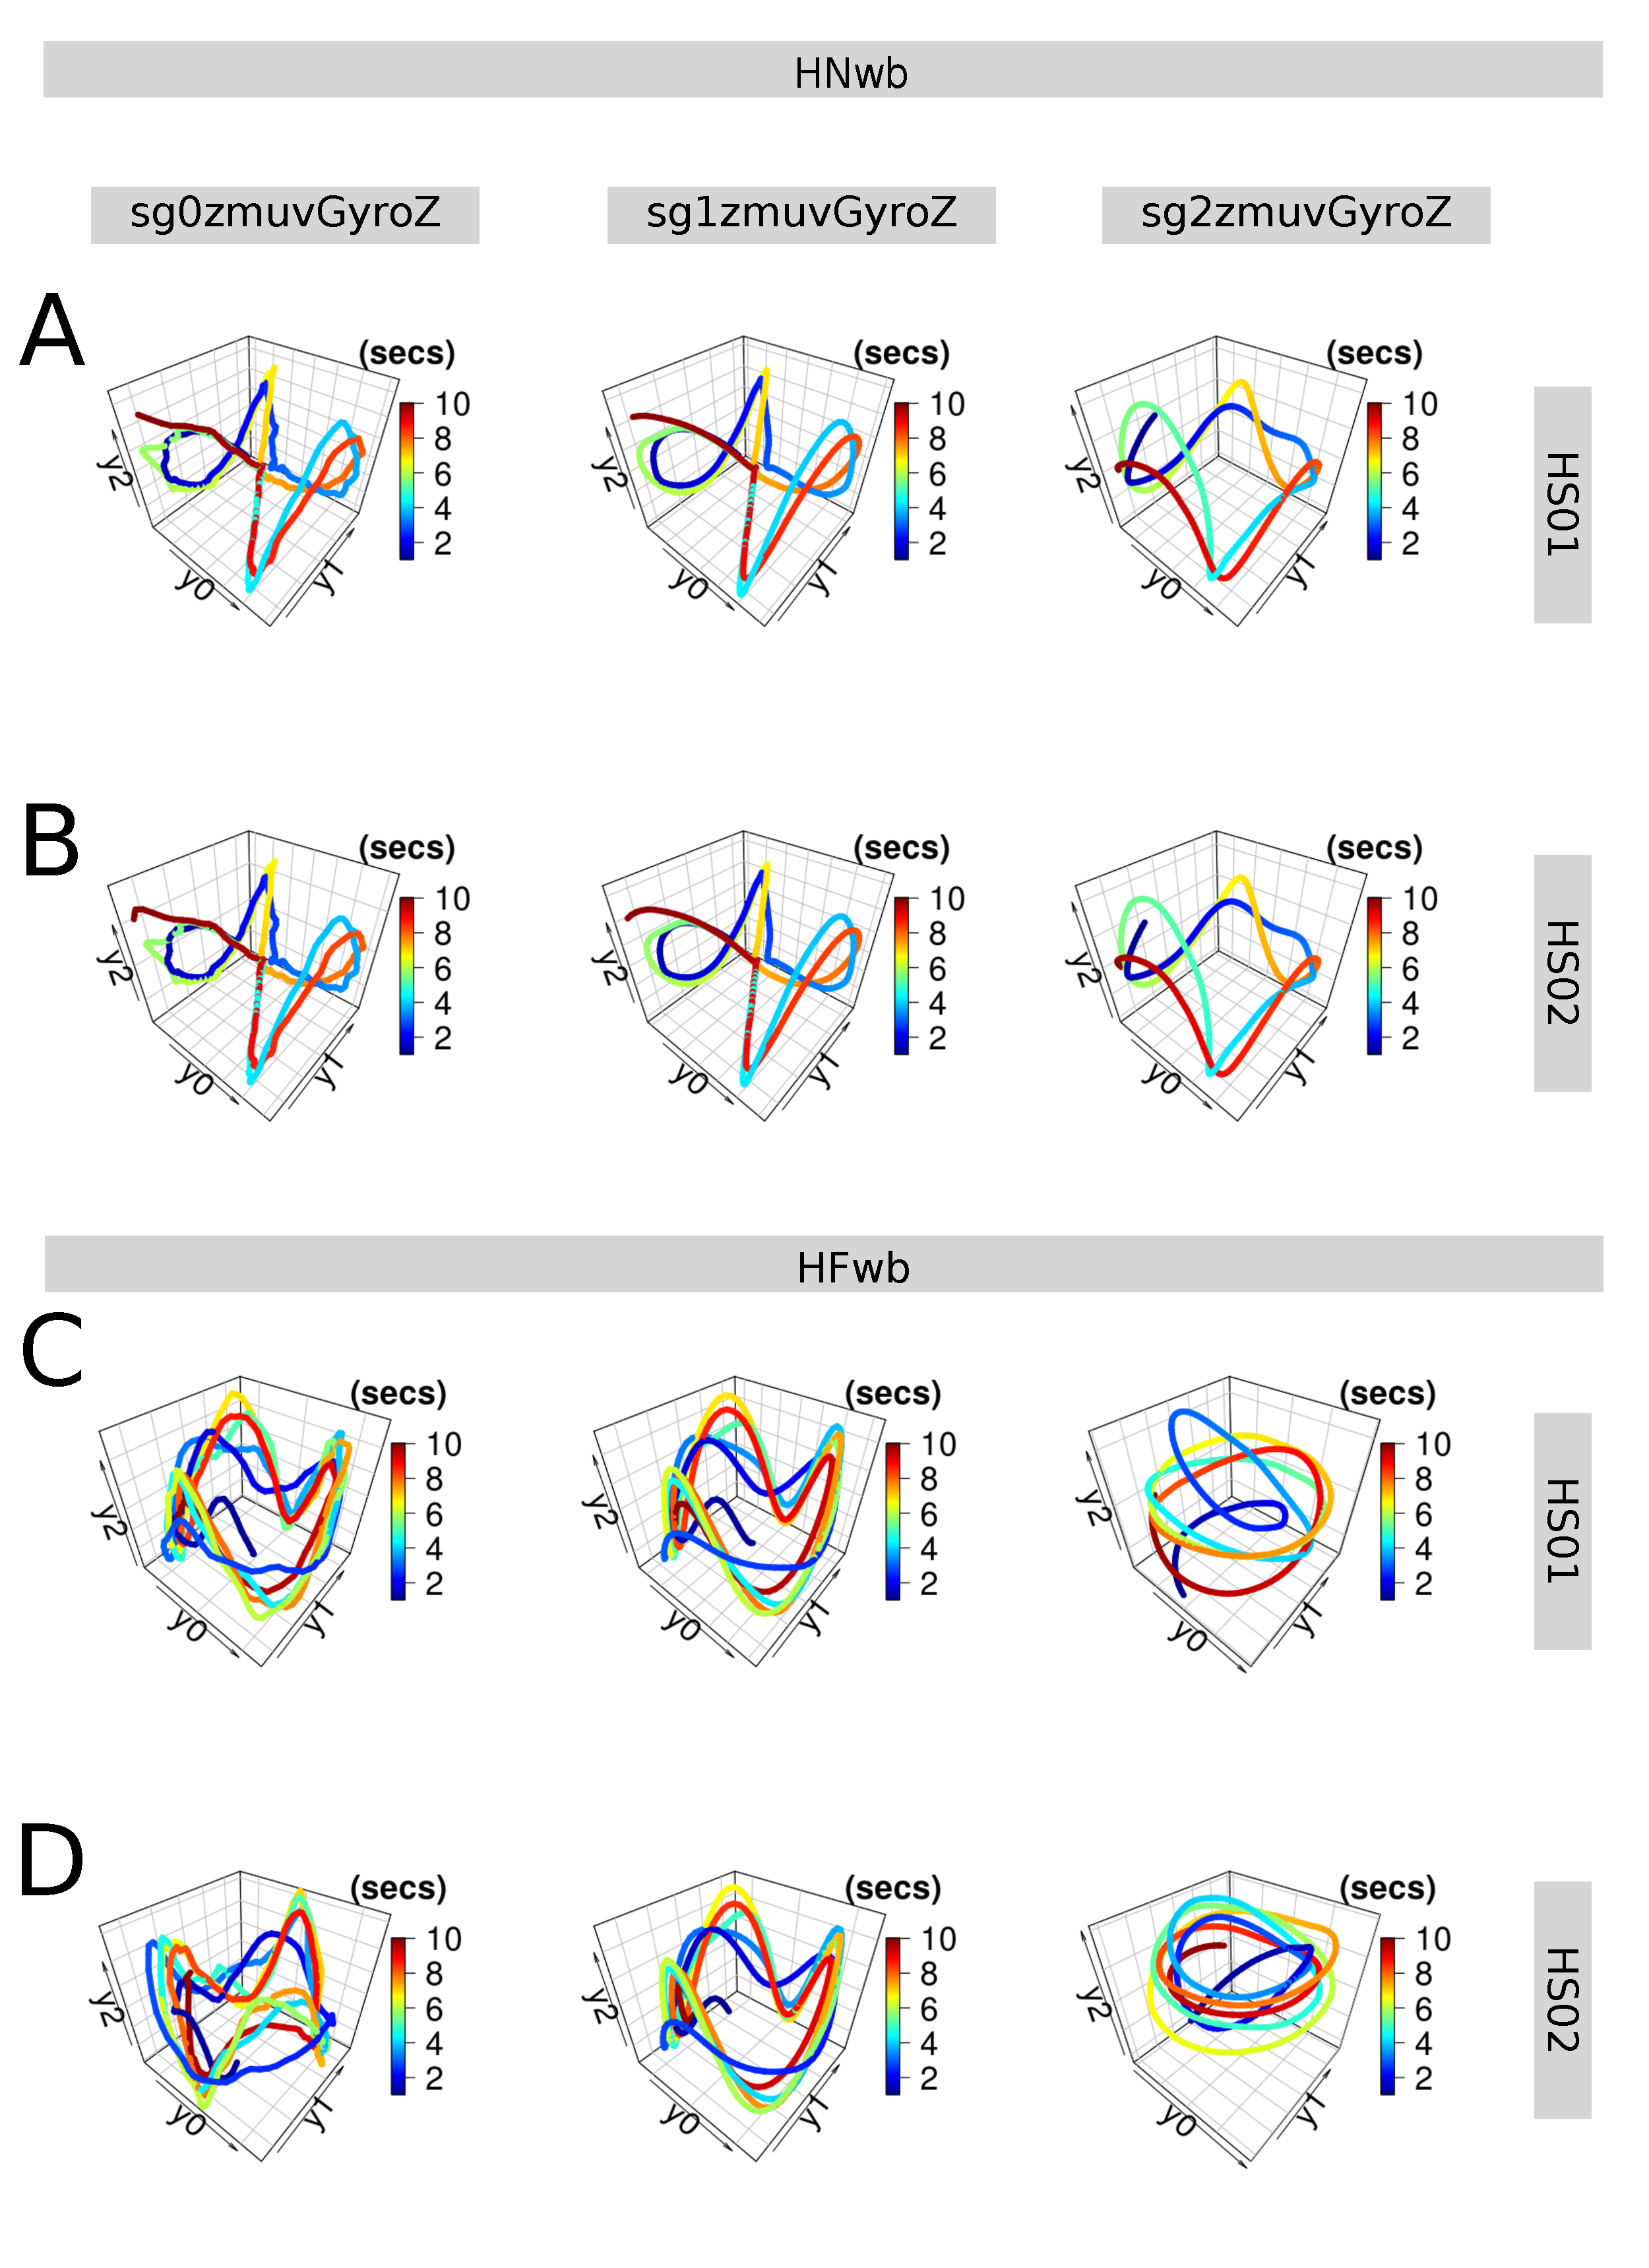
\includegraphics[height=0.8\textheight]{fig_5_06}
\caption
	[RSSs for horizontal arm movements (with beat)]{
	{\bf RSSs for horizontal arm movements (with beat).}
	Reconstructed state spaces of participant p01 for 
	(A, B) horizontal normal movements with beat (HNwb) and 
	(C, D) horizontal faster velocity with beat (HFwb).
	Time series for raw-normalised (sg0zmuvGyroZ), 
	normalised-smoothed 1 (sg1zmuvGyroZ) and 
	normalised-smoothed 2 (sg2zmuvGyroZ) with
	(A, C) sensor attached to the participant (HS01), and
	(B, D) sensor attached to the participant (HS02).	
	Reconstructed state spaces were computed with 
	embedding parameters $\overline{m_0}=6$, $\overline{\tau_0}=10$.
	\R code to reproduce the figure is available at 
	\codelink{
	https://github.com/mxochicale-phd/thesis/tree/master/0_code_data/1_code/7_figs_ch5/04_fig5.5-5.6-5.7-5.8/code
	}.
        }
     \label{fig:rss_Hwb_w500}
\end{figure}
%%---------------------------------(FIGURE)------------------------------------

%%---------------------------------(FIGURE)-------------------------------------
\begin{figure}
\centering
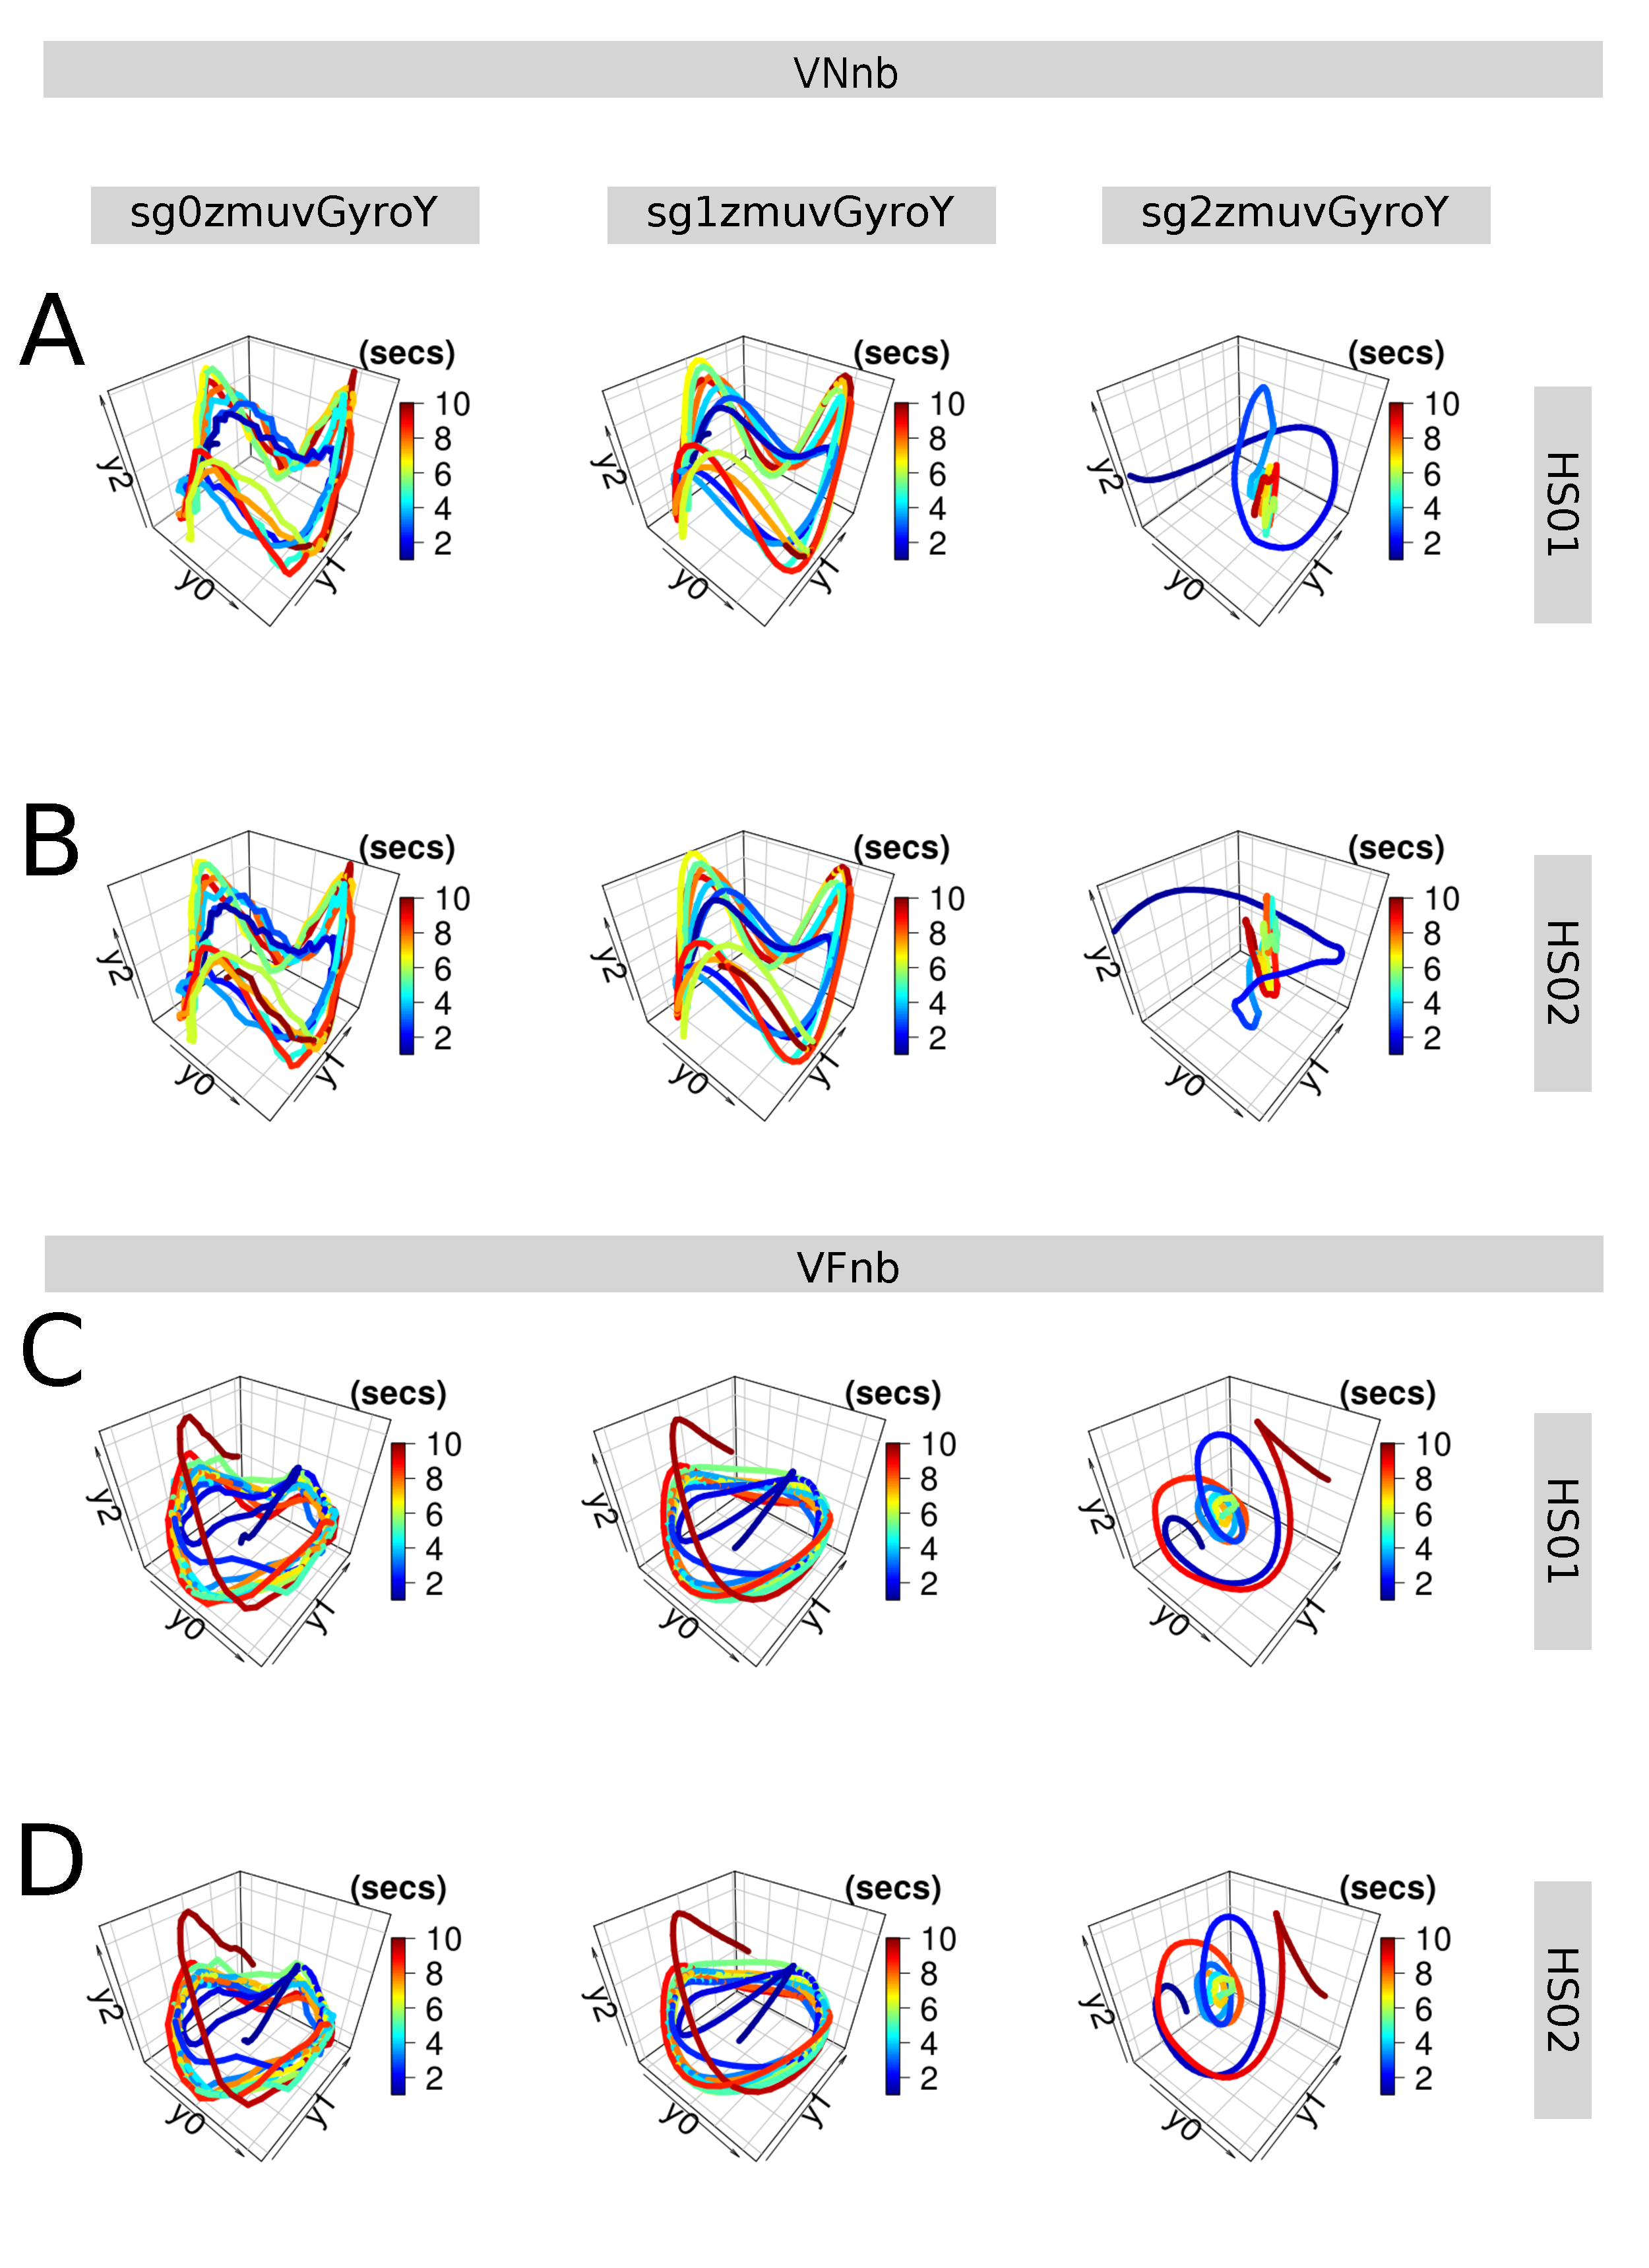
\includegraphics[height=0.8\textheight]{fig_5_07}
\caption
	[RSSs for vertical arm movements (no beat)]{
	{\bf RSSs for vertical arm movements (no beat).}
	Reconstructed state spaces of participant p01 for 
	(A, B) vertical normal movements with no beat (VNnb) and 
	(C, D) vertical faster velocity with no beat (VFnb).
	Time series for raw-normalised (sg0zmuvGyroY), 
	normalised-smoothed 1 (sg1zmuvGyroY) and 
	normalised-smoothed 2 (sg2zmuvGyroY) with
	(A, C) sensor attached to the participant (HS01), and
	(B, D) sensor attached to the participant (HS02).	
	Reconstructed state spaces were computed with 
	embedding parameters $\overline{m_0}=6$, $\overline{\tau_0}=10$.
	\R code to reproduce the figure is available at 
	\codelink{
	https://github.com/mxochicale-phd/thesis/tree/master/0_code_data/1_code/7_figs_ch5/04_fig5.5-5.6-5.7-5.8/code
	}.
        }
     \label{fig:rss_Vnb_w500}
\end{figure}
%%---------------------------------(FIGURE)------------------------------------

%%---------------------------------(FIGURE)-------------------------------------
\begin{figure}
\centering
\includegraphics[height=0.8\textheight]{fig_5_08}
\caption
	[RSSs for vertical arm movements (with beat)]{
	{\bf RSSs for vertical arm movements (with beat).}
	Reconstructed state spaces of participant p01 for 
	(A, B) vertical normal movements with beat (VNwb) and 
	(C, D) vertical faster velocity with beat (VFwb).
	Time series for raw-normalised (sg0zmuvGyroY), 
	normalised-smoothed 1 (sg1zmuvGyroY) and 
	normalised-smoothed 2 (sg2zmuvGyroY) with
	(A, C) sensor attached to the participant (HS01), and
	(B, D) sensor attached to the participant (HS02).	
	Reconstructed state spaces were computed with 
	embedding parameters $\overline{m_0}=6$, $\overline{\tau_0}=10$.
	\R code to reproduce the figure is available at 
	\codelink{
	https://github.com/mxochicale-phd/thesis/tree/master/0_code_data/1_code/7_figs_ch5/04_fig5.5-5.6-5.7-5.8/code
	}.
        }
     \label{fig:rss_Vwb_w500}
\end{figure}
%%---------------------------------(FIGURE)------------------------------------

\newpage
\section{Recurrences Plots}
Patterns of recurrence plots (RPs) are described in this section.
Recurrence plots are computed with embedding parameters 
$\overline{m_0}=6$, $\overline{\tau_0}=10$ and a recurrence 
threshold $\epsilon=1$ for participant $p01$ performing horizontal 
and vertical arm movements in normal and faster velocity 
with beat and no beat sound (Figs \ref{fig:rps_Hnb_w500}, 
\ref{fig:rps_Hwb_w500}, \ref{fig:rps_Vnb_w500} and \ref{fig:rps_Vwb_w500}).

Figs \ref{fig:rps_Hnb_w500} show recurrence plots for horizontal normal
and horizontal faster arm movements with no beat sound. 
For horizontal normal arm movements with no beat, patterns in 
RPs for sg0zmuvGyroZ and sg1zmuvGyroZ look similar, however
patterns in RPs for sg2zmuvGyroZ are different,
such behavior of RPs patterns is similar with regards to the smoothness 
presented in horizontal and faster arm movements with beat
(Fig \ref{fig:rps_Hwb_w500}).
With regards to the type of sensor, there is little visual differences in 
RPs patters, while patterns of RPs for different activities present diagonal 
lines that appear to be closer and more dense for horizontal faster 
arm movement than horizontal normal arm movements (Fig \ref{fig:rps_Hnb_w500}).

Figs \ref{fig:rps_Hwb_w500} show patterns of RPs for horizontal normal
and faster arm movements while participants listen to a beat. 
For these patterns in the RPs, the type activities for normal and 
faster arm movements can be easily noticed in the patterns,
as well as the change of smoothness between sg0zmuvGyroZ and sg1zmuvGyroZ
with the patterns for sg2zmuvGyroZ. It can also noted that there is 
little visual differences between the RP patters for sensor HS01 and HS02.

Figs \ref{fig:rps_Vnb_w500} show patterns of RPs for vertical normal
and faster arm movements while no hearing a beat. One can note
the evidently differences of patterns between the levels of smoothness 
where, for instance, patterns of RPs from sg0zmuvGyroY and sg1zmuvGyroY 
looks similar while RPs for sg2zmuvGyroY are completely black.
Similarly, one can see little visual changes when comparing RPs patterns 
between sensors HS01 and HS02. 
However, the RPs patterns create a more dense presence of diagonal lines
for faster arm movements than for normal arm movements. 

Figs \ref{fig:rps_Vwb_w500} show RPs patterns for vertical normal and 
faster arm movements for participants hearing a beat. 
Patterns of RP for vertical normal and vertical faster arm movements are 
visually noticeable as well as RPs patterns for changes in 
the increase of smoothness between sg0zmuvGyroY and sg1zmuvGyroY and 
with sg2zmuvGyroY. Once can also note that there is little visual 
changes of RPs patterns from different sensors.
%%---------------------------------(FIGURE)------------------------------------
\begin{figure}
\centering
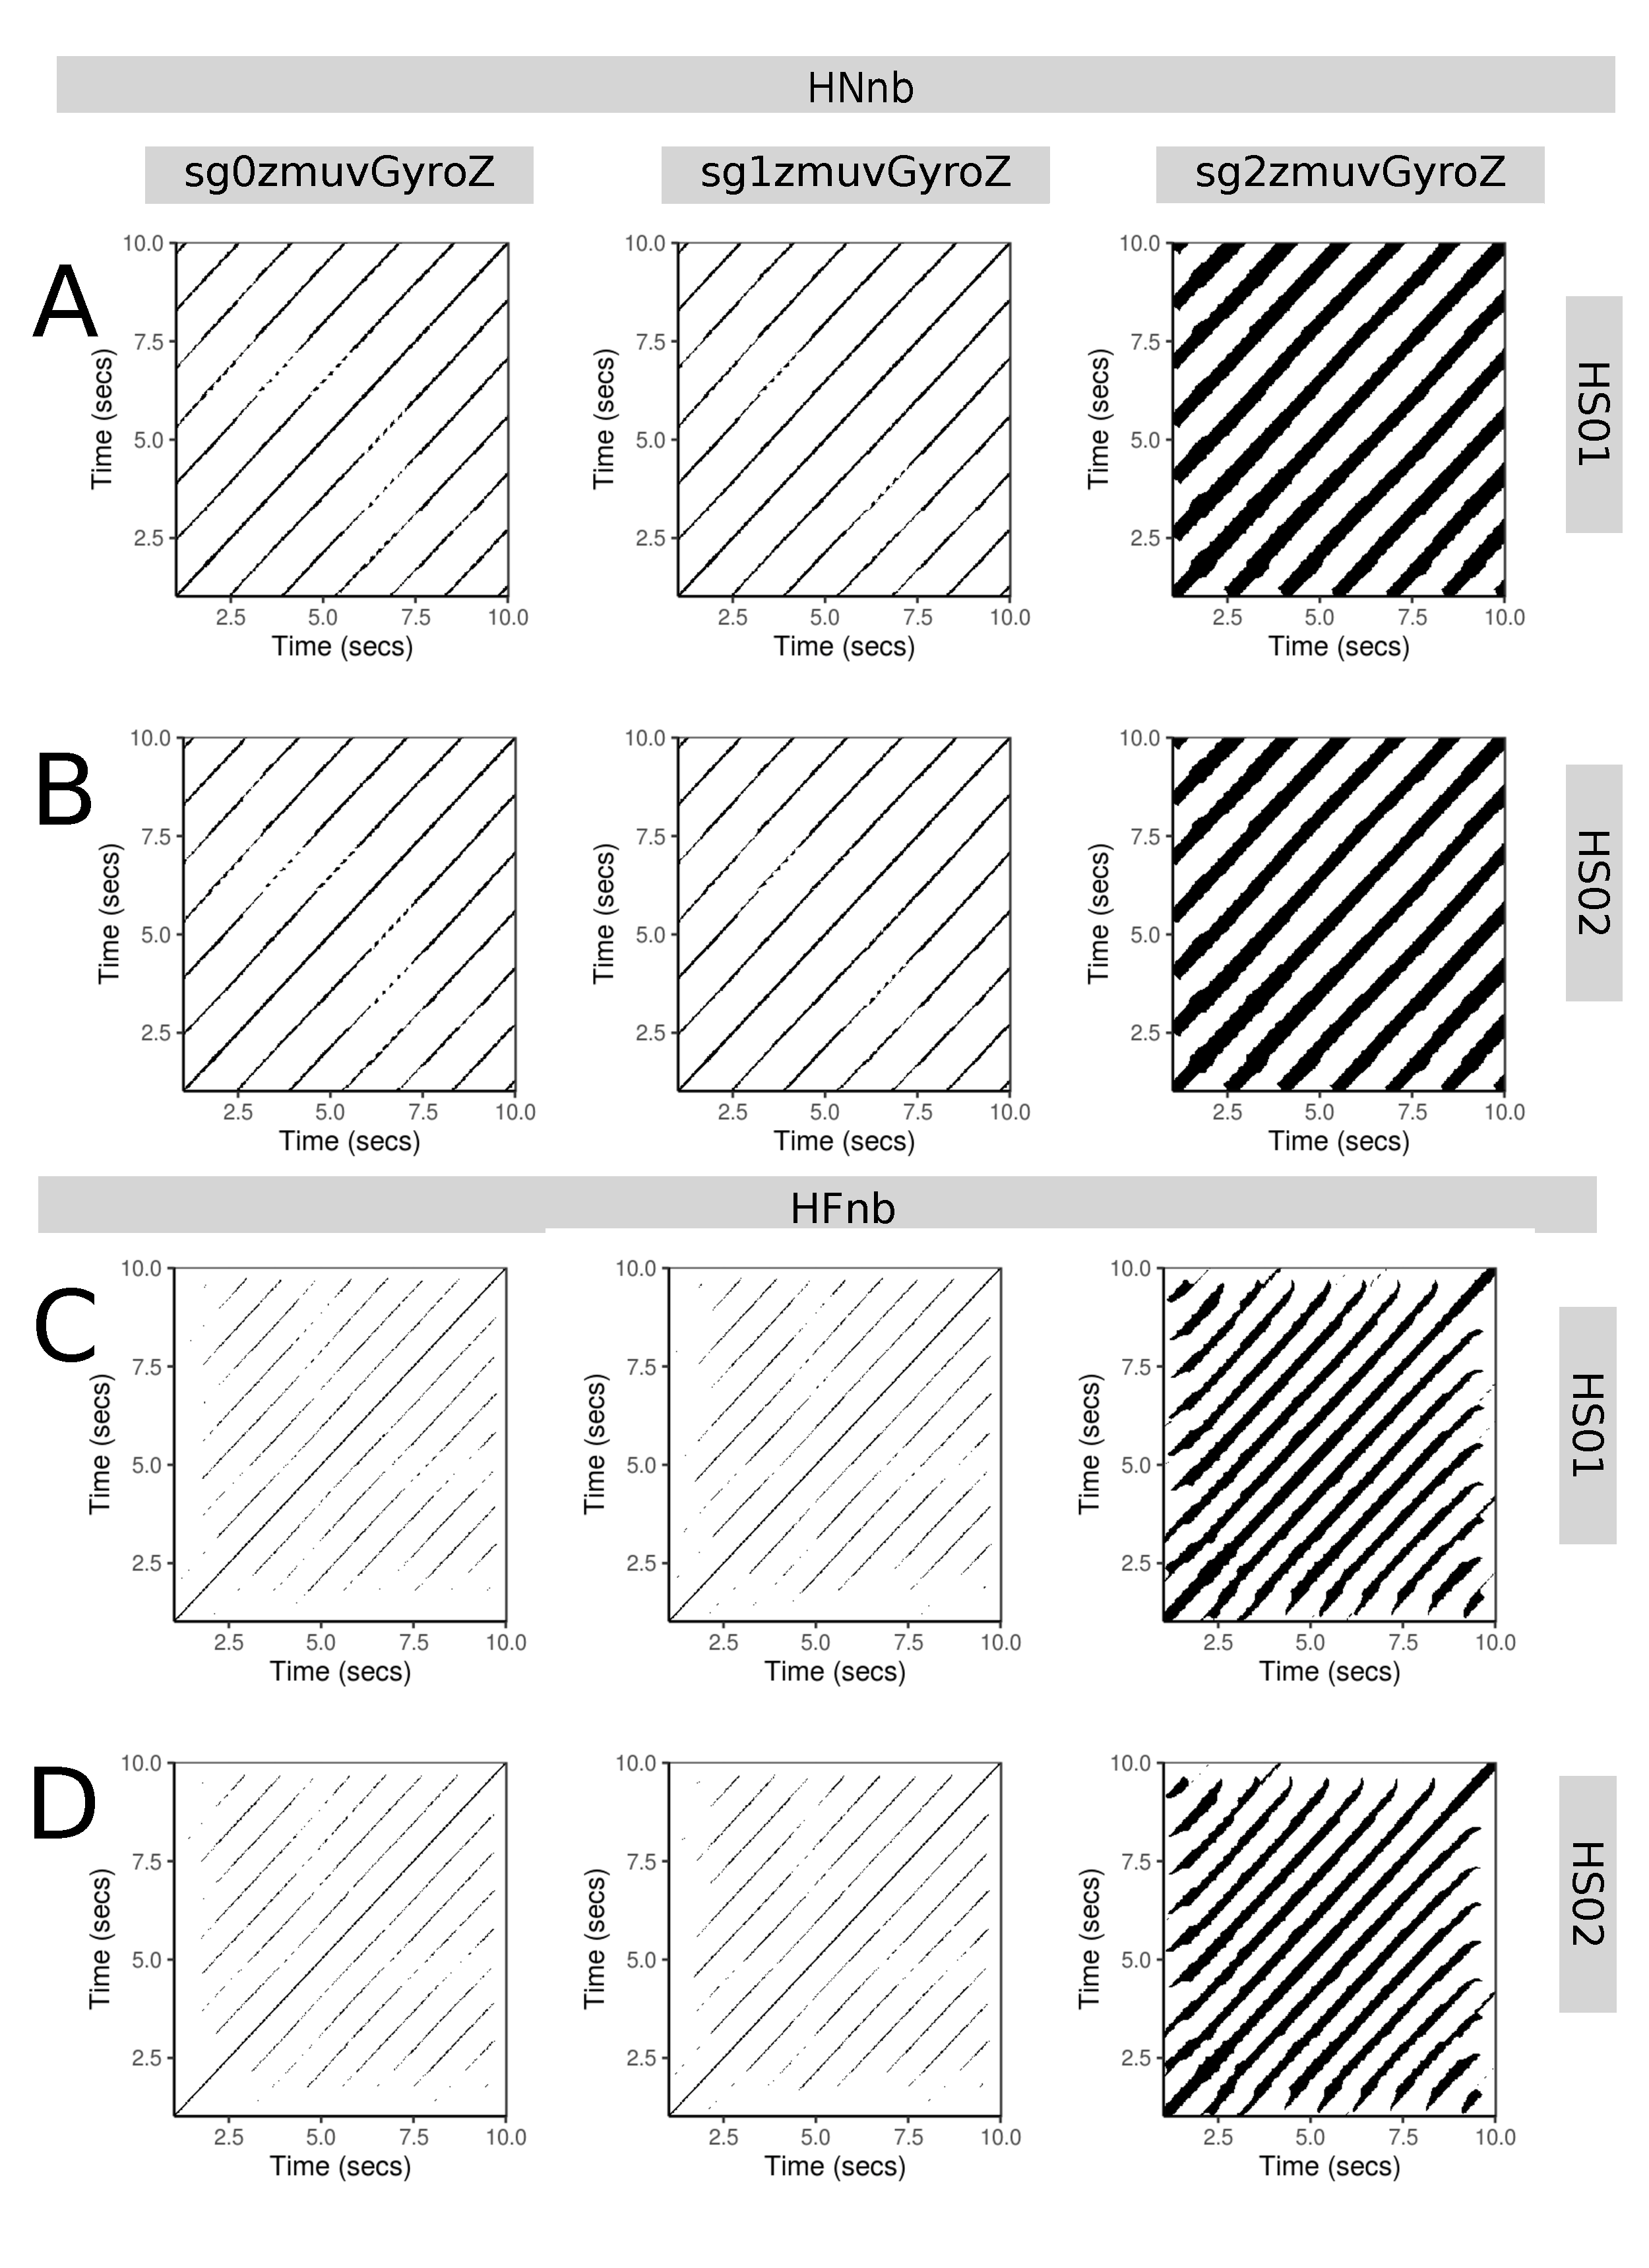
\includegraphics[height=0.8\textheight]{fig_5_09}
\caption
	[RPs for horizontal arm movements (no beat)]{
	{\bf RPs for horizontal arm movements (no beat).}	
	Recurrence plots of participant p01 for 
	(A, B) horizontal normal movements with no beat (HNnb) and
	(C, D) horizontal faster movements with no beat (HFnb).
	Time series for raw-normalised (sg0zmuvGyroZ), 
	normalised-smoothed 1 (sg1zmuvGyroZ) and 
	normalised-smoothed 2 (sg2zmuvGyroZ) with
	(A, C) sensor 01 attached to the participant (HS01), and
	(B, D) sensor 02 attached to the participant (HS02).
	Recurrence plots were computed with 
	embedding parameters $\overline{m_0}=6$, $\overline{\tau_0}=10$ and 
	recurrence threshold $\epsilon=1$.
	\R code to reproduce the figure is available at 
	\codelink{
	https://github.com/mxochicale-phd/thesis/tree/master/0_code_data/1_code/7_figs_ch5/05_fig5.9-5.10-5.11-5.12/code
	}.
        }
    \label{fig:rps_Hnb_w500}
\end{figure}
%%---------------------------------(FIGURE)------------------------------------
%%---------------------------------(FIGURE)------------------------------------
\begin{figure}
\centering
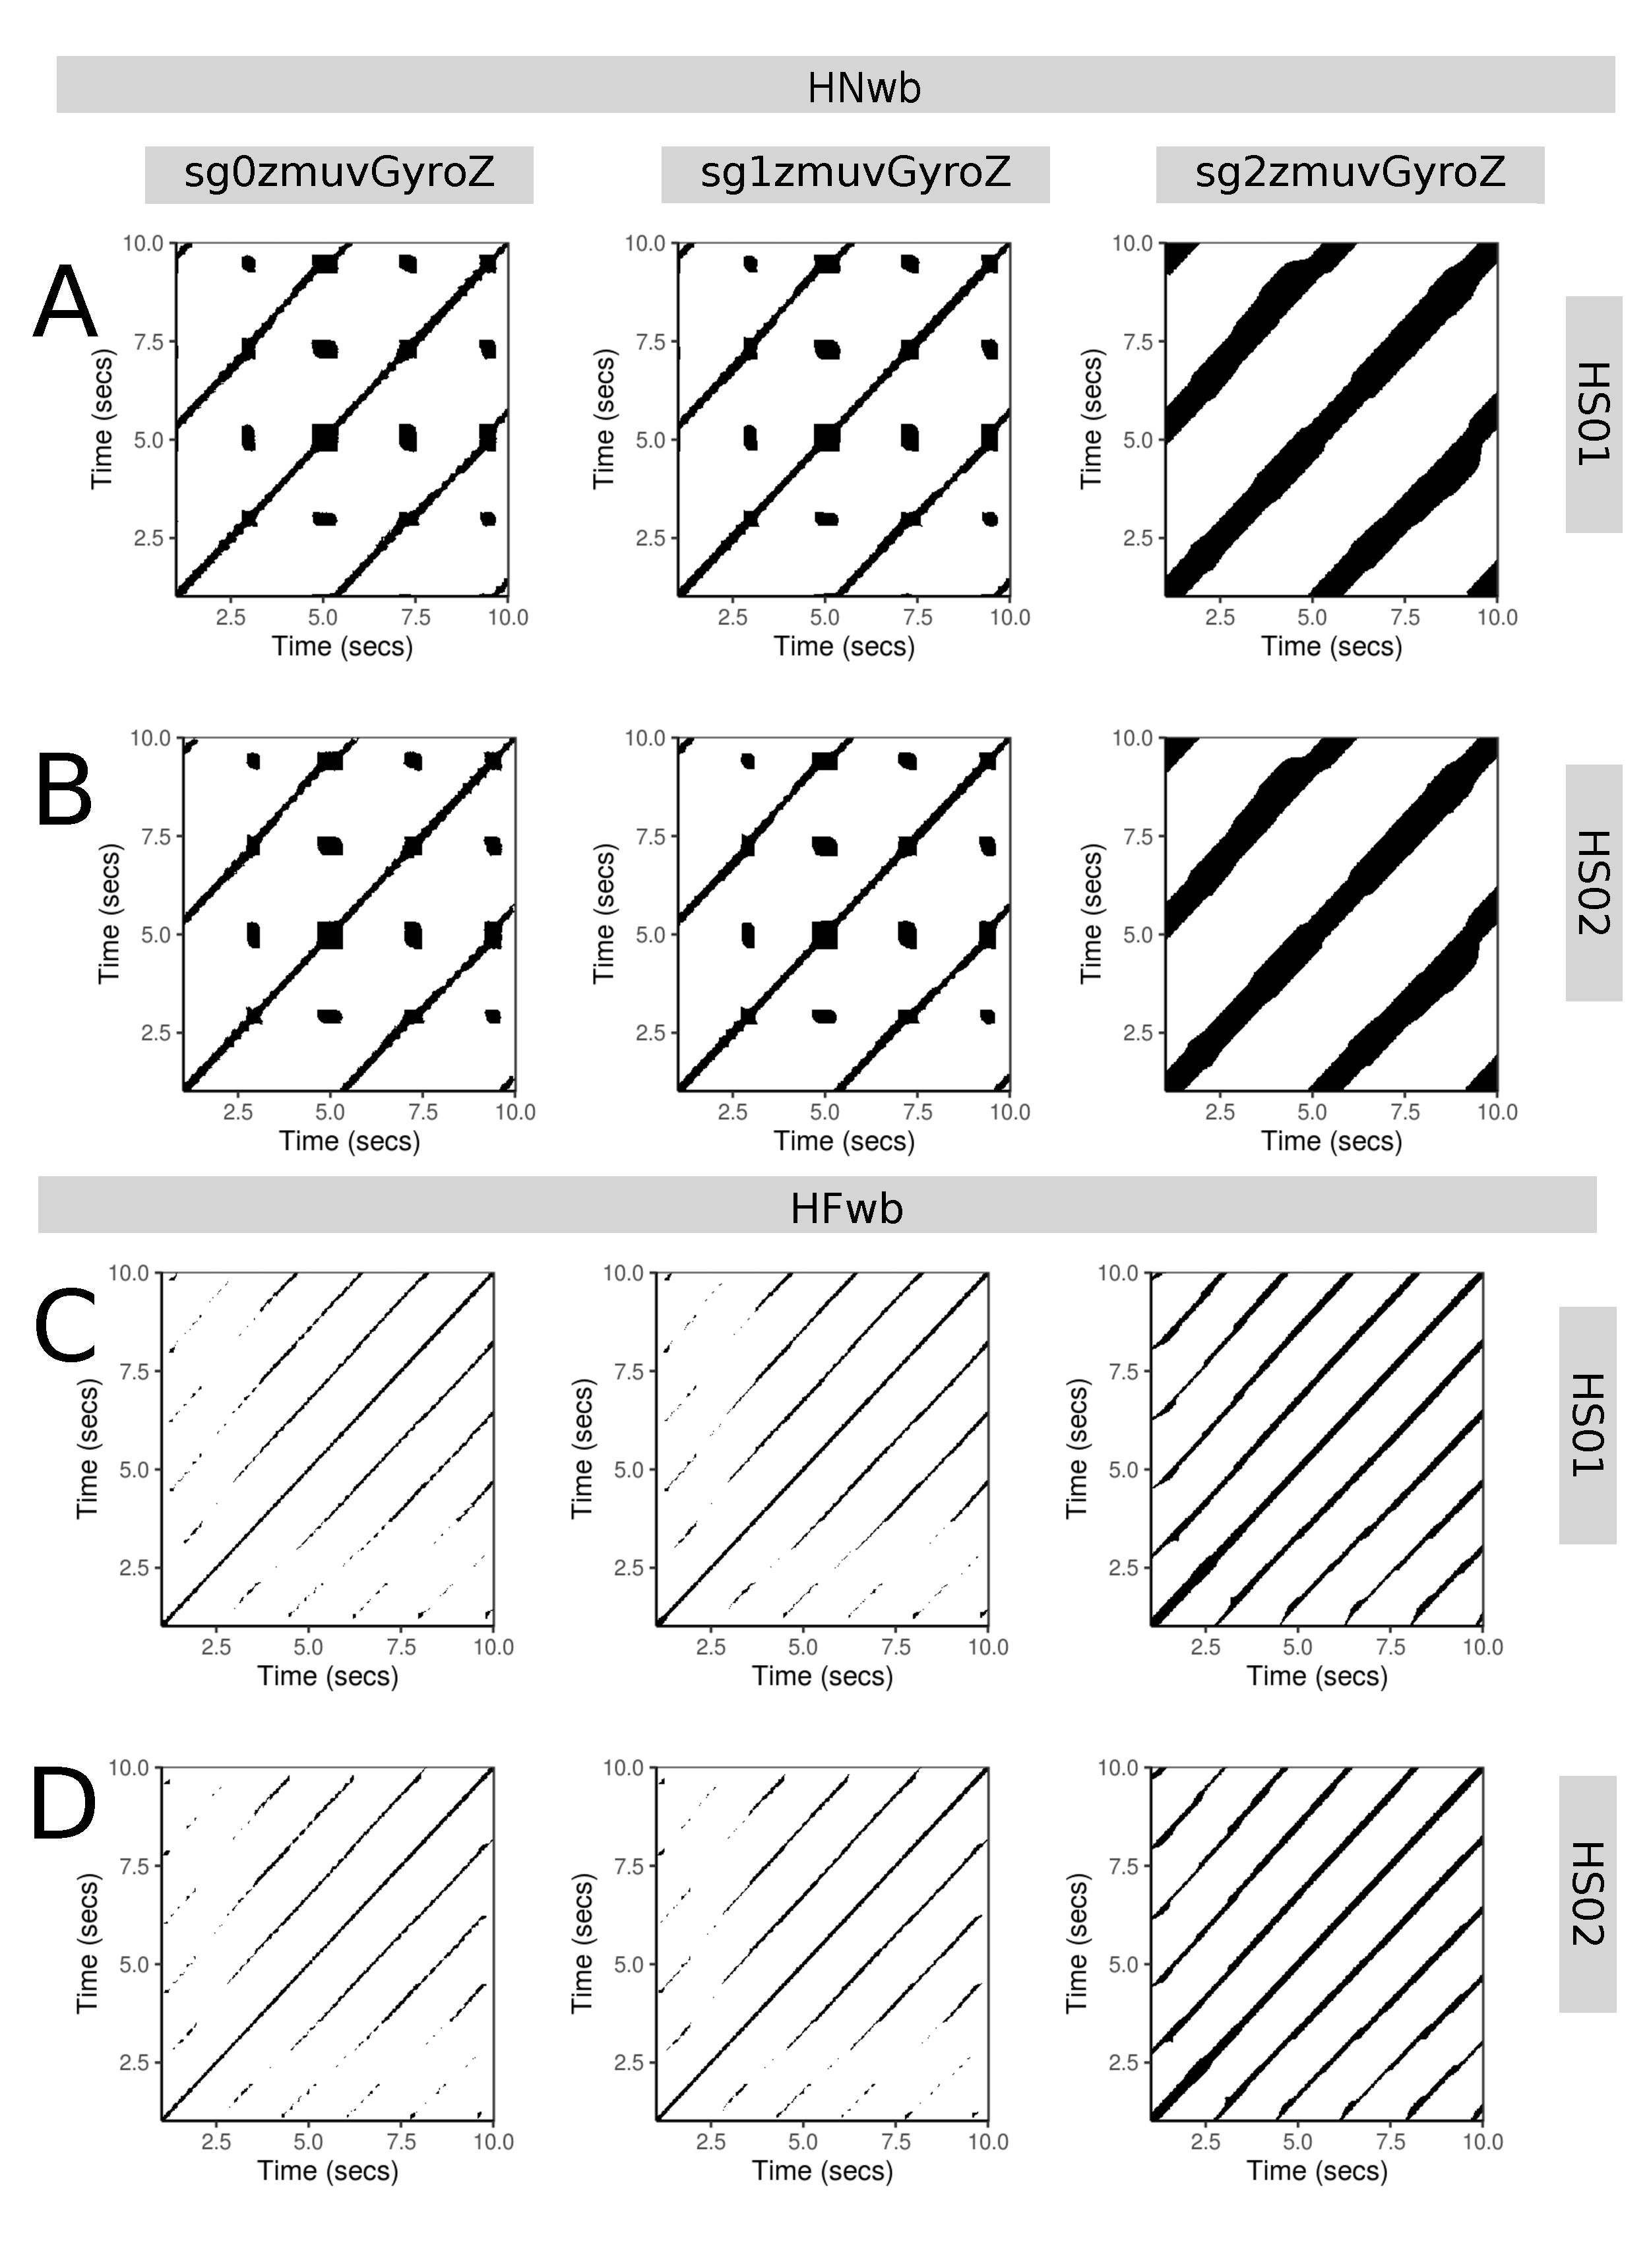
\includegraphics[height=0.8\textheight]{fig_5_10}
\caption
	[RPs for horizontal arm movements (with beat)]{
	{\bf RPs for horizontal arm movements (with beat).}	
	Recurrence plots of participant p01 for 
	(A, B) horizontal normal movements with beat (HNwb) and
	(C, D) horizontal faster movements with beat (HFwb).
	Time series for raw-normalised (sg0zmuvGyroZ), 
	normalised-smoothed 1 (sg1zmuvGyroZ) and 
	normalised-smoothed 2 (sg2zmuvGyroZ) with
	(A, C) sensor 01 attached to the participant (HS01), and
	(B, D) sensor 02 attached to the participant (HS02).
	Recurrence plots were computed with 
	embedding parameters $\overline{m_0}=6$, $\overline{\tau_0}=10$ and 
	recurrence threshold $\epsilon=1$.
	\R code to reproduce the figure is available at 
	\codelink{
	https://github.com/mxochicale-phd/thesis/tree/master/0_code_data/1_code/7_figs_ch5/05_fig5.9-5.10-5.11-5.12/code
	}.
        }
    \label{fig:rps_Hwb_w500}
\end{figure}
%%---------------------------------(FIGURE)------------------------------------
%%---------------------------------(FIGURE)-----------------------------------
\begin{figure}
\centering
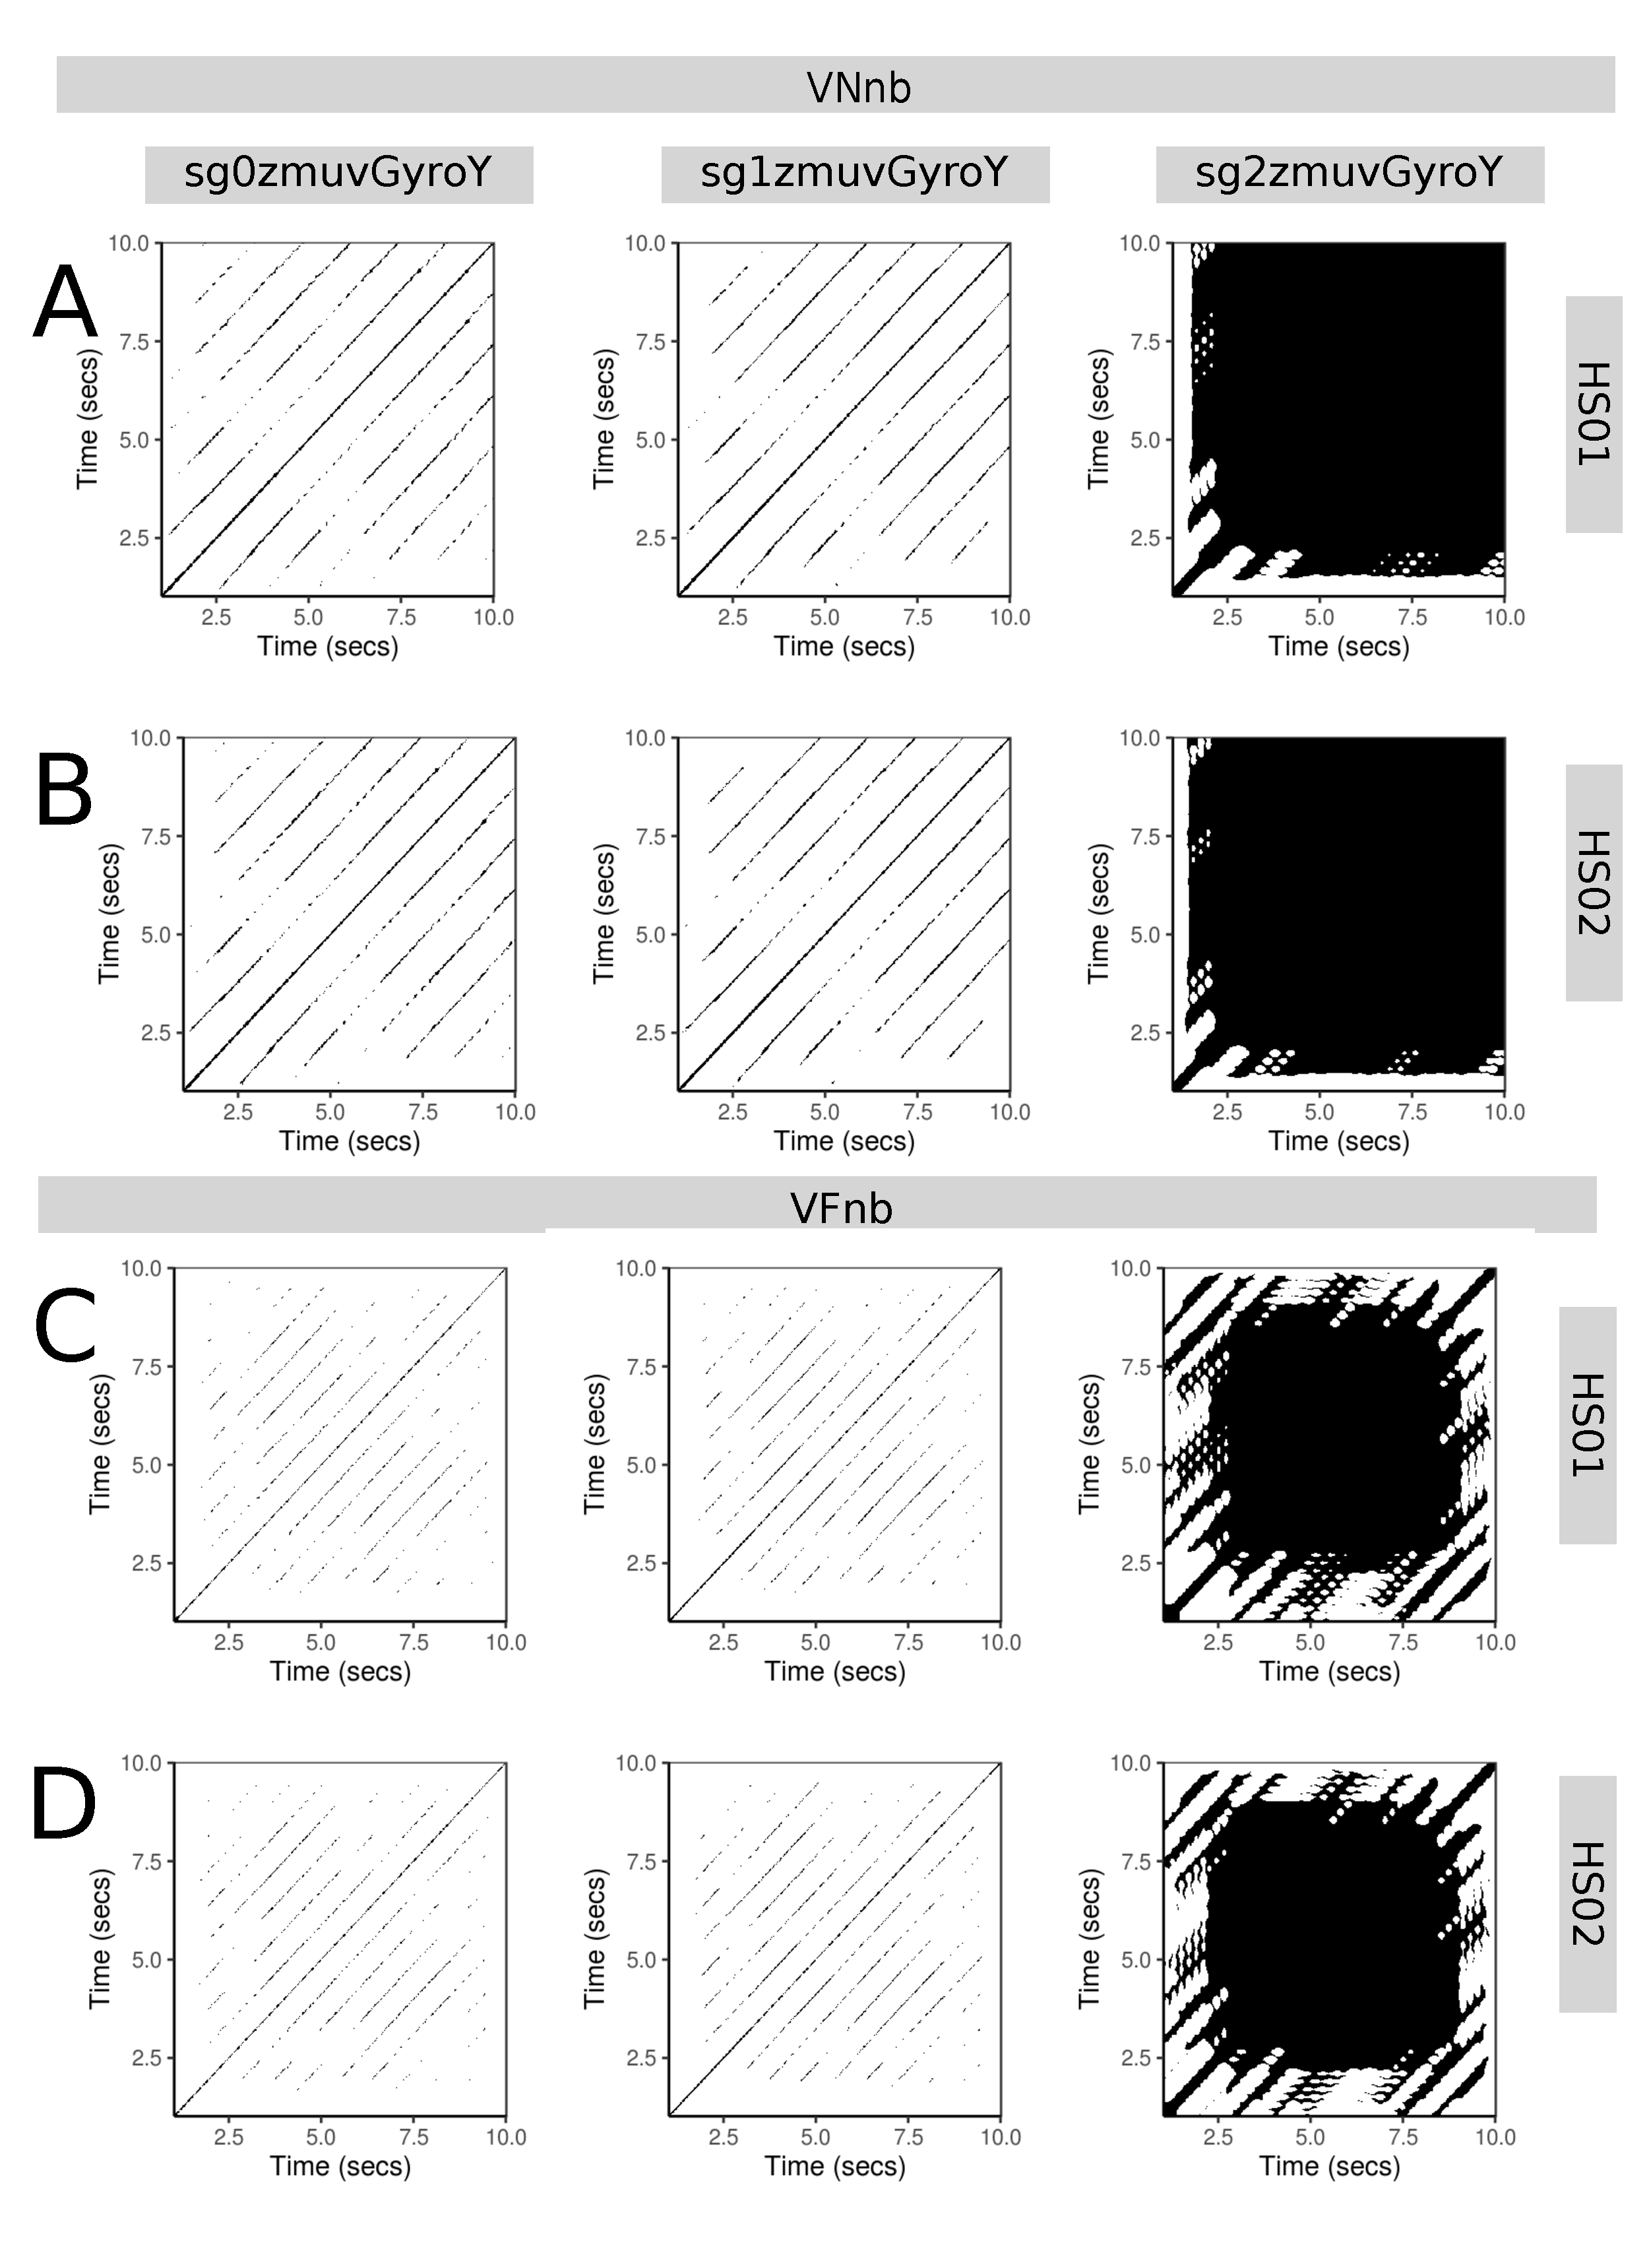
\includegraphics[height=0.8\textheight]{fig_5_11}
\caption
	[RPs for vertical arm movements (no beat)]{
	{\bf RPs for vertical arm movements (no beat).}	
	Recurrence plots of participant p01 for 
	(A, B) vertical normal movements with no beat (VNnb) and
	(C, D) vertical faster movements with no beat (VFnb).
	Time series for raw-normalised (sg0zmuvGyroY), 
	normalised-smoothed 1 (sg1zmuvGyroY) and 
	normalised-smoothed 2 (sg2zmuvGyroY) with
	(A, C) sensor 01 attached to the participant (HS01), and
	(B, D) sensor 02 attached to the participant (HS02).
	Recurrence plots were computed with 
	embedding parameters $\overline{m_0}=6$, $\overline{\tau_0}=10$ and 
	recurrence threshold $\epsilon=1$.
	\R code to reproduce the figure is available at 
	\codelink{
	https://github.com/mxochicale-phd/thesis/tree/master/0_code_data/1_code/7_figs_ch5/05_fig5.9-5.10-5.11-5.12/code
	}.
        }
    \label{fig:rps_Vnb_w500}
\end{figure}
%%---------------------------------(FIGURE)------------------------------------
%%---------------------------------(FIGURE)-----------------------------------
\begin{figure}
\centering
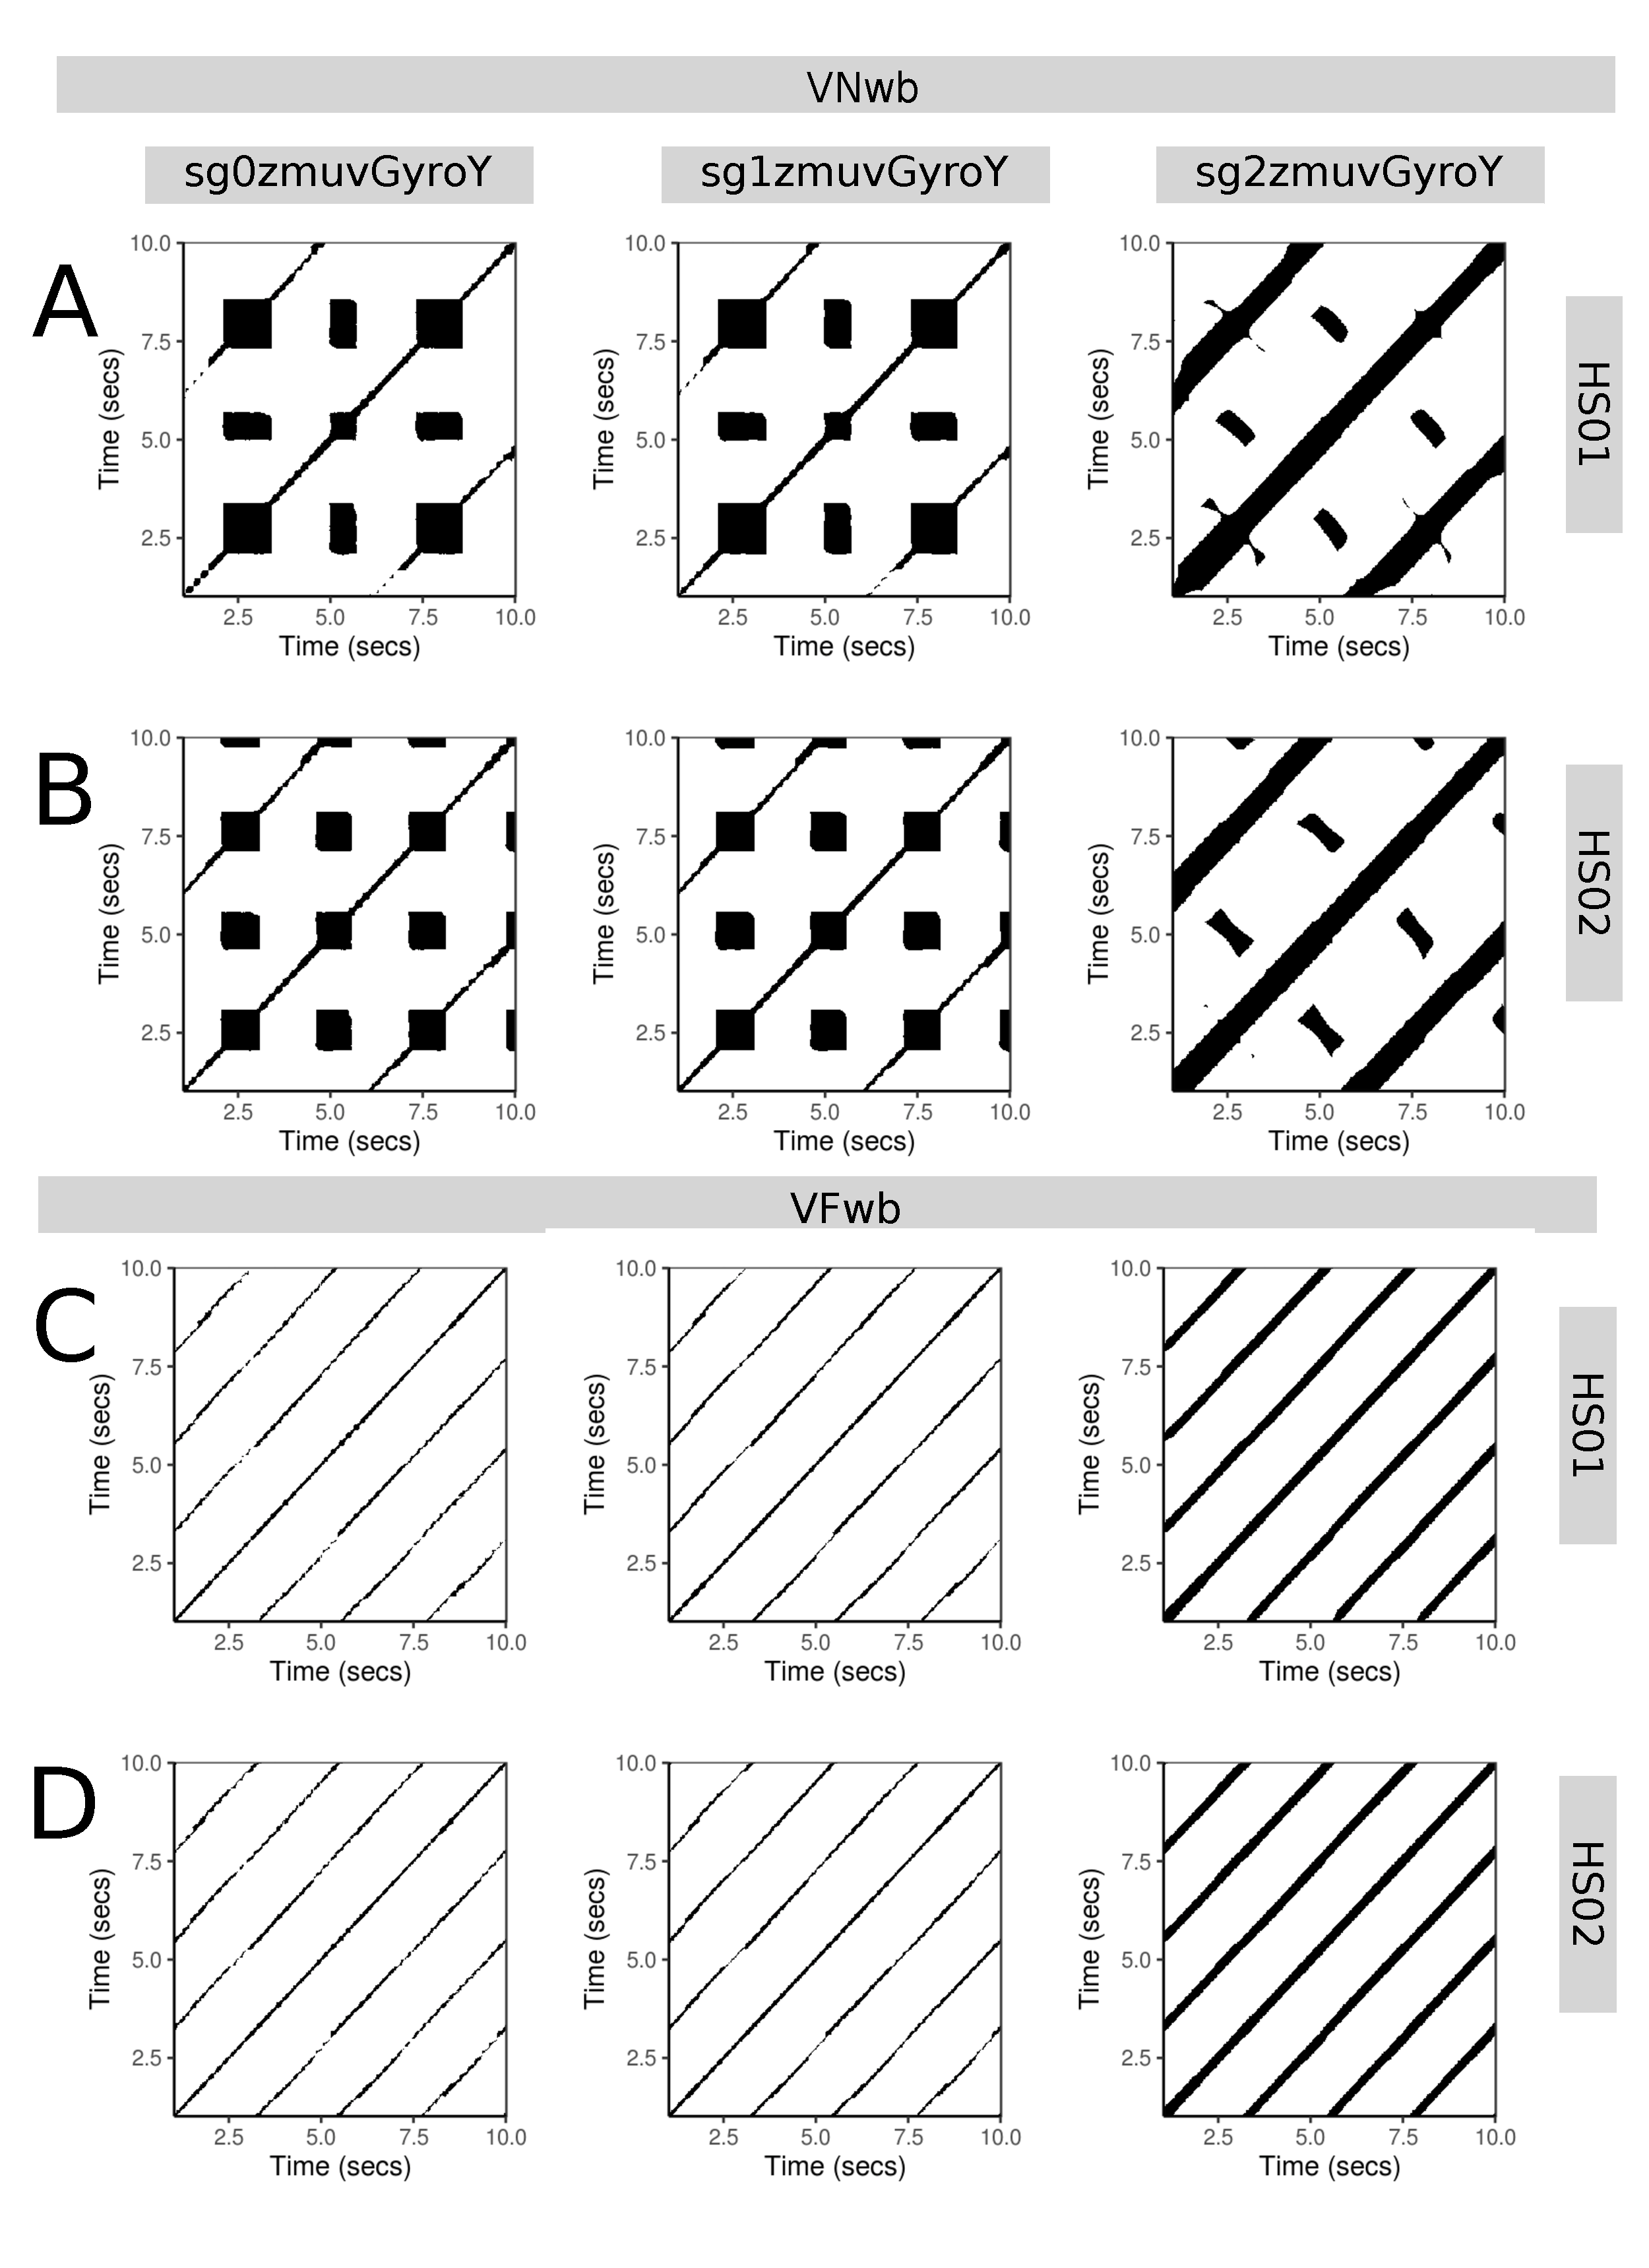
\includegraphics[height=0.8\textheight]{fig_5_12}
\caption
	[RPs for vertical arm movements (with beat)]{
	{\bf RPs for vertical arm movements (with beat).}	
	Recurrence plots of participant p01 for 
	(A, B) vertical normal movements with beat (VNwb) and
	(C, D) vertical faster movements with beat (VFwb).
	Time series for raw-normalised (sg0zmuvGyroY), 
	normalised-smoothed 1 (sg1zmuvGyroY) and 
	normalised-smoothed 2 (sg2zmuvGyroY) with
	(A, C) sensor 01 attached to the participant (HS01), and
	(B, D) sensor 02 attached to the participant (HS02).
	Recurrence plots were computed with 
	embedding parameters $\overline{m_0}=6$, $\overline{\tau_0}=10$ and 
	recurrence threshold $\epsilon=1$.
	\R code to reproduce the figure is available at 
	\codelink{
	https://github.com/mxochicale-phd/thesis/tree/master/0_code_data/1_code/7_figs_ch5/05_fig5.9-5.10-5.11-5.12/code
	}.
        }
    \label{fig:rps_Vwb_w500}
\end{figure}
%%---------------------------------(FIGURE)------------------------------------

\newpage
\section{Recurrence Quantification Analysis} \label{ch5:rqas}
In this section is shown Recurrence Quantification Analysis (RQA) metrics 
(REC, DET, RATIO and ENTR) of six participants ($p01, p04, p05, p10, p11, p15$)
for horizontal arm movements (HNnb, HNwb, HFnb, HFwb) 
and vertical arm movements (VNnb, VNwb, VFnb, VFwb)  
with sensors HS01 and HS02, and three smoothed time series 
(sg0zmuvGyro, sg1zmuvGyro and  sg2zmuvGyro).
I hence compute four metrics of RQA metrics (REC, DET, RATIO and ENTR) with 
embedding parameters $\overline{m_0}=6$, $\overline{\tau_0}=10$ and 
recurrence threshold $\epsilon=1$.
 
\subsection*{REC values}
Figs \ref{fig:BPRQAH}(A) and \ref{fig:BPRQAV}(A) 
show box plots of REC values, representing \% of black 
dots in the RPs, for horizontal arm movements and 
vertical arm movements. 
In figs \ref{fig:BPRQAH}(A) can be noted that the interquartile range for sg2 
is greater than the sg0 and sg1 for activities HNnb and HFnb, while
REC values for activities HNwb and HFwb appear to increase 
its sample mean (gray rhombus) as the smoothness increase.
Similarly, in figs \ref{fig:BPRQAV}(A) can be seen that there is a large 
interquartile range for sg2 in activities with no beat (VNnb, VFnb), while
activities with beat (VNwb and VFwb) appear to be increase its sample
mean (gray rhombus) as the smoothness of the time series increase. 
REC values from sensors HS01 and HS01 appear to differ little 
for both horizontal and vertical arm movements. 
For further details of individual REC values of participants, see 
Figs \ref{fig:rqa_rec_H} and \ref{fig:rqa_rec_V} in 
Section \ref{appendix:e:rpas}.

\subsection*{DET values}
DET values, representing predictability and organisation of the RPs, appear
to be constant irregardless of the source of time series 
(Figs \ref{fig:BPRQAH}(B) and \ref{fig:BPRQAV}(B) ).
However, it can be noted a slight increase of DET values as the 
smoothness increase.
For further details of individual DET values of participants, see 
Figs \ref{fig:rqa_det_H}, \ref{fig:rqa_det_V} in
Section \ref{appendix:e:rpas}.

\subsection*{RATIO values}
RATIO values, representing dynamics transitions, for horizontal and 
vertical arm movements are shown in Figs 
\ref{fig:BPRQAH}(C) and \ref{fig:BPRQAV}(C).
In Figs \ref{fig:BPRQAH}(C), for vertical arm movements, 
can be noted that HNwb activity
present the less interquartile range while other seem to have similar
interquartile range. Also, the increase of smoothness makes RATIO
values to decrease (see gray rhombus).
Similarly, in Figs \ref{fig:BPRQAV}(C), for vertical arm movements, 
is shown that VNwb has the less interquartile range as well as 
sg2 for VFnb and VFwb activities. 
The increase of smoothness of time series affect in the way that 
the sample mean values of RATIO values (gray rhombus) decrease. 
For further details of individual DET values of participants, see 
Figs \ref{fig:rqa_ratio_H}, \ref{fig:rqa_ratio_V} in
Section \ref{appendix:e:rpas}.

\subsection*{ENTR values}
Figs \ref{fig:BPRQAH}(D) and \ref{fig:BPRQAV}(D) show ENTR values, 
representing the complexity of the structure of time series, 
for horizontal and vertical arm movements.
Generally, figs \ref{fig:BPRQAH}(D) and \ref{fig:BPRQAV}(D) 
illustrate that the increase of smoothness causes an increase of 
sample mean (gray rhombus) of ENTR values in each of 
the activities and sensors. 
For both vertical and horizontal ENTR values for Nwb seems 
to be a bit higher than Nnb, while Fnb and Fwb appear to be 
have similar values.
Also, there is little change between HS01 and HS02 sensors.
For further details of individual ENTR values of participants, see 
Figs \ref{fig:rqa_entr_H}, \ref{fig:rqa_entr_V} in
Section \ref{appendix:e:rpas}.

%%---------------------------------(FIGURE)-------------------------------------
\begin{figure}
\centering
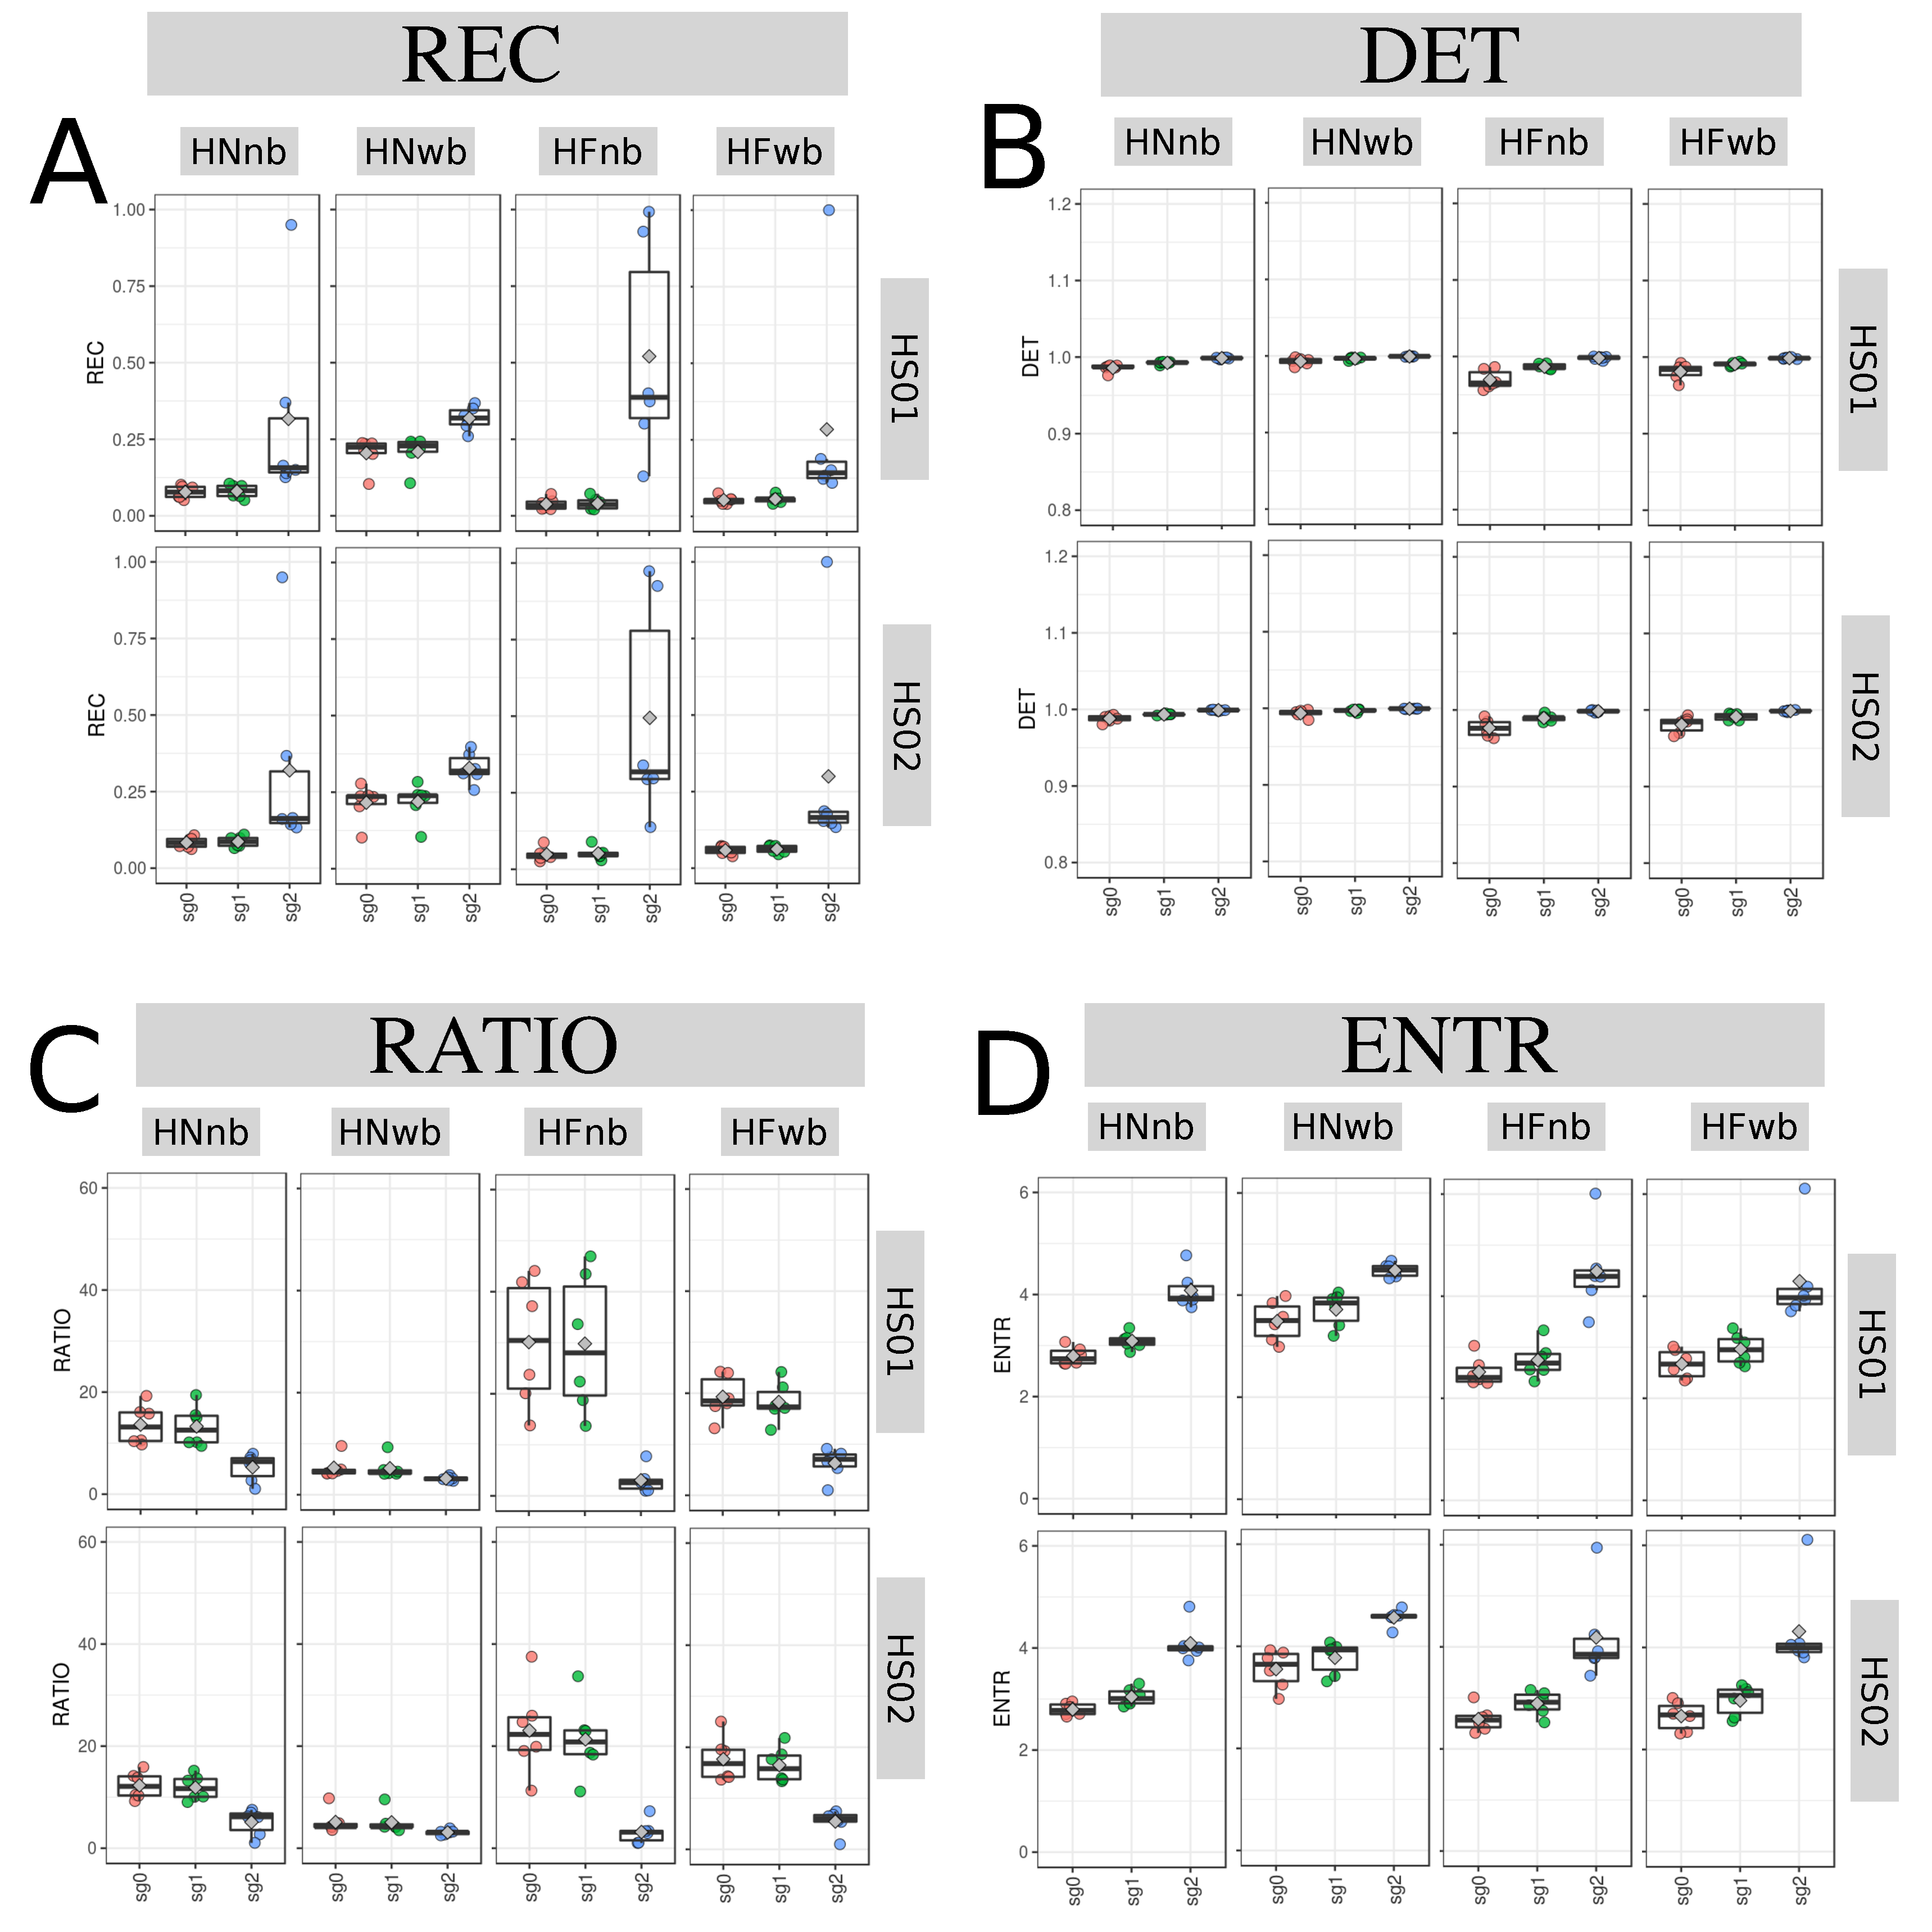
\includegraphics[width=1.0\textwidth]{fig_5_13}
	\caption
	[Box plots of RQA values for horizontal arm movements]{
	{\bf Box plots of RQA values for horizontal arm movements.}
	Box plots of (A) REC, (B) DET, (C) RATIO, and (D) ENTR values 
	for 6 participants performing HNnb, HNwb, HFnb and HFwb movements
	with sensors HS01, HS02 and three smoothed-normalised  
	time series (sg0, sg1 and sg2).
	RQA values were computed with 
	embedding parameters $\overline{m_0}=6$, $\overline{\tau_0}=10$ and 
	recurrence threshold $\epsilon=1$.
	\R code to reproduce the figure is available at 
	\codelink{
	https://github.com/mxochicale-phd/thesis/tree/master/0_code_data/1_code/7_figs_ch5/06_fig5.13-5.14/code
	}.
        }
    \label{fig:BPRQAH}
\end{figure}
%%---------------------------------(FIGURE)-------------------------------------

%%---------------------------------(FIGURE)-------------------------------------
\begin{figure}
\centering
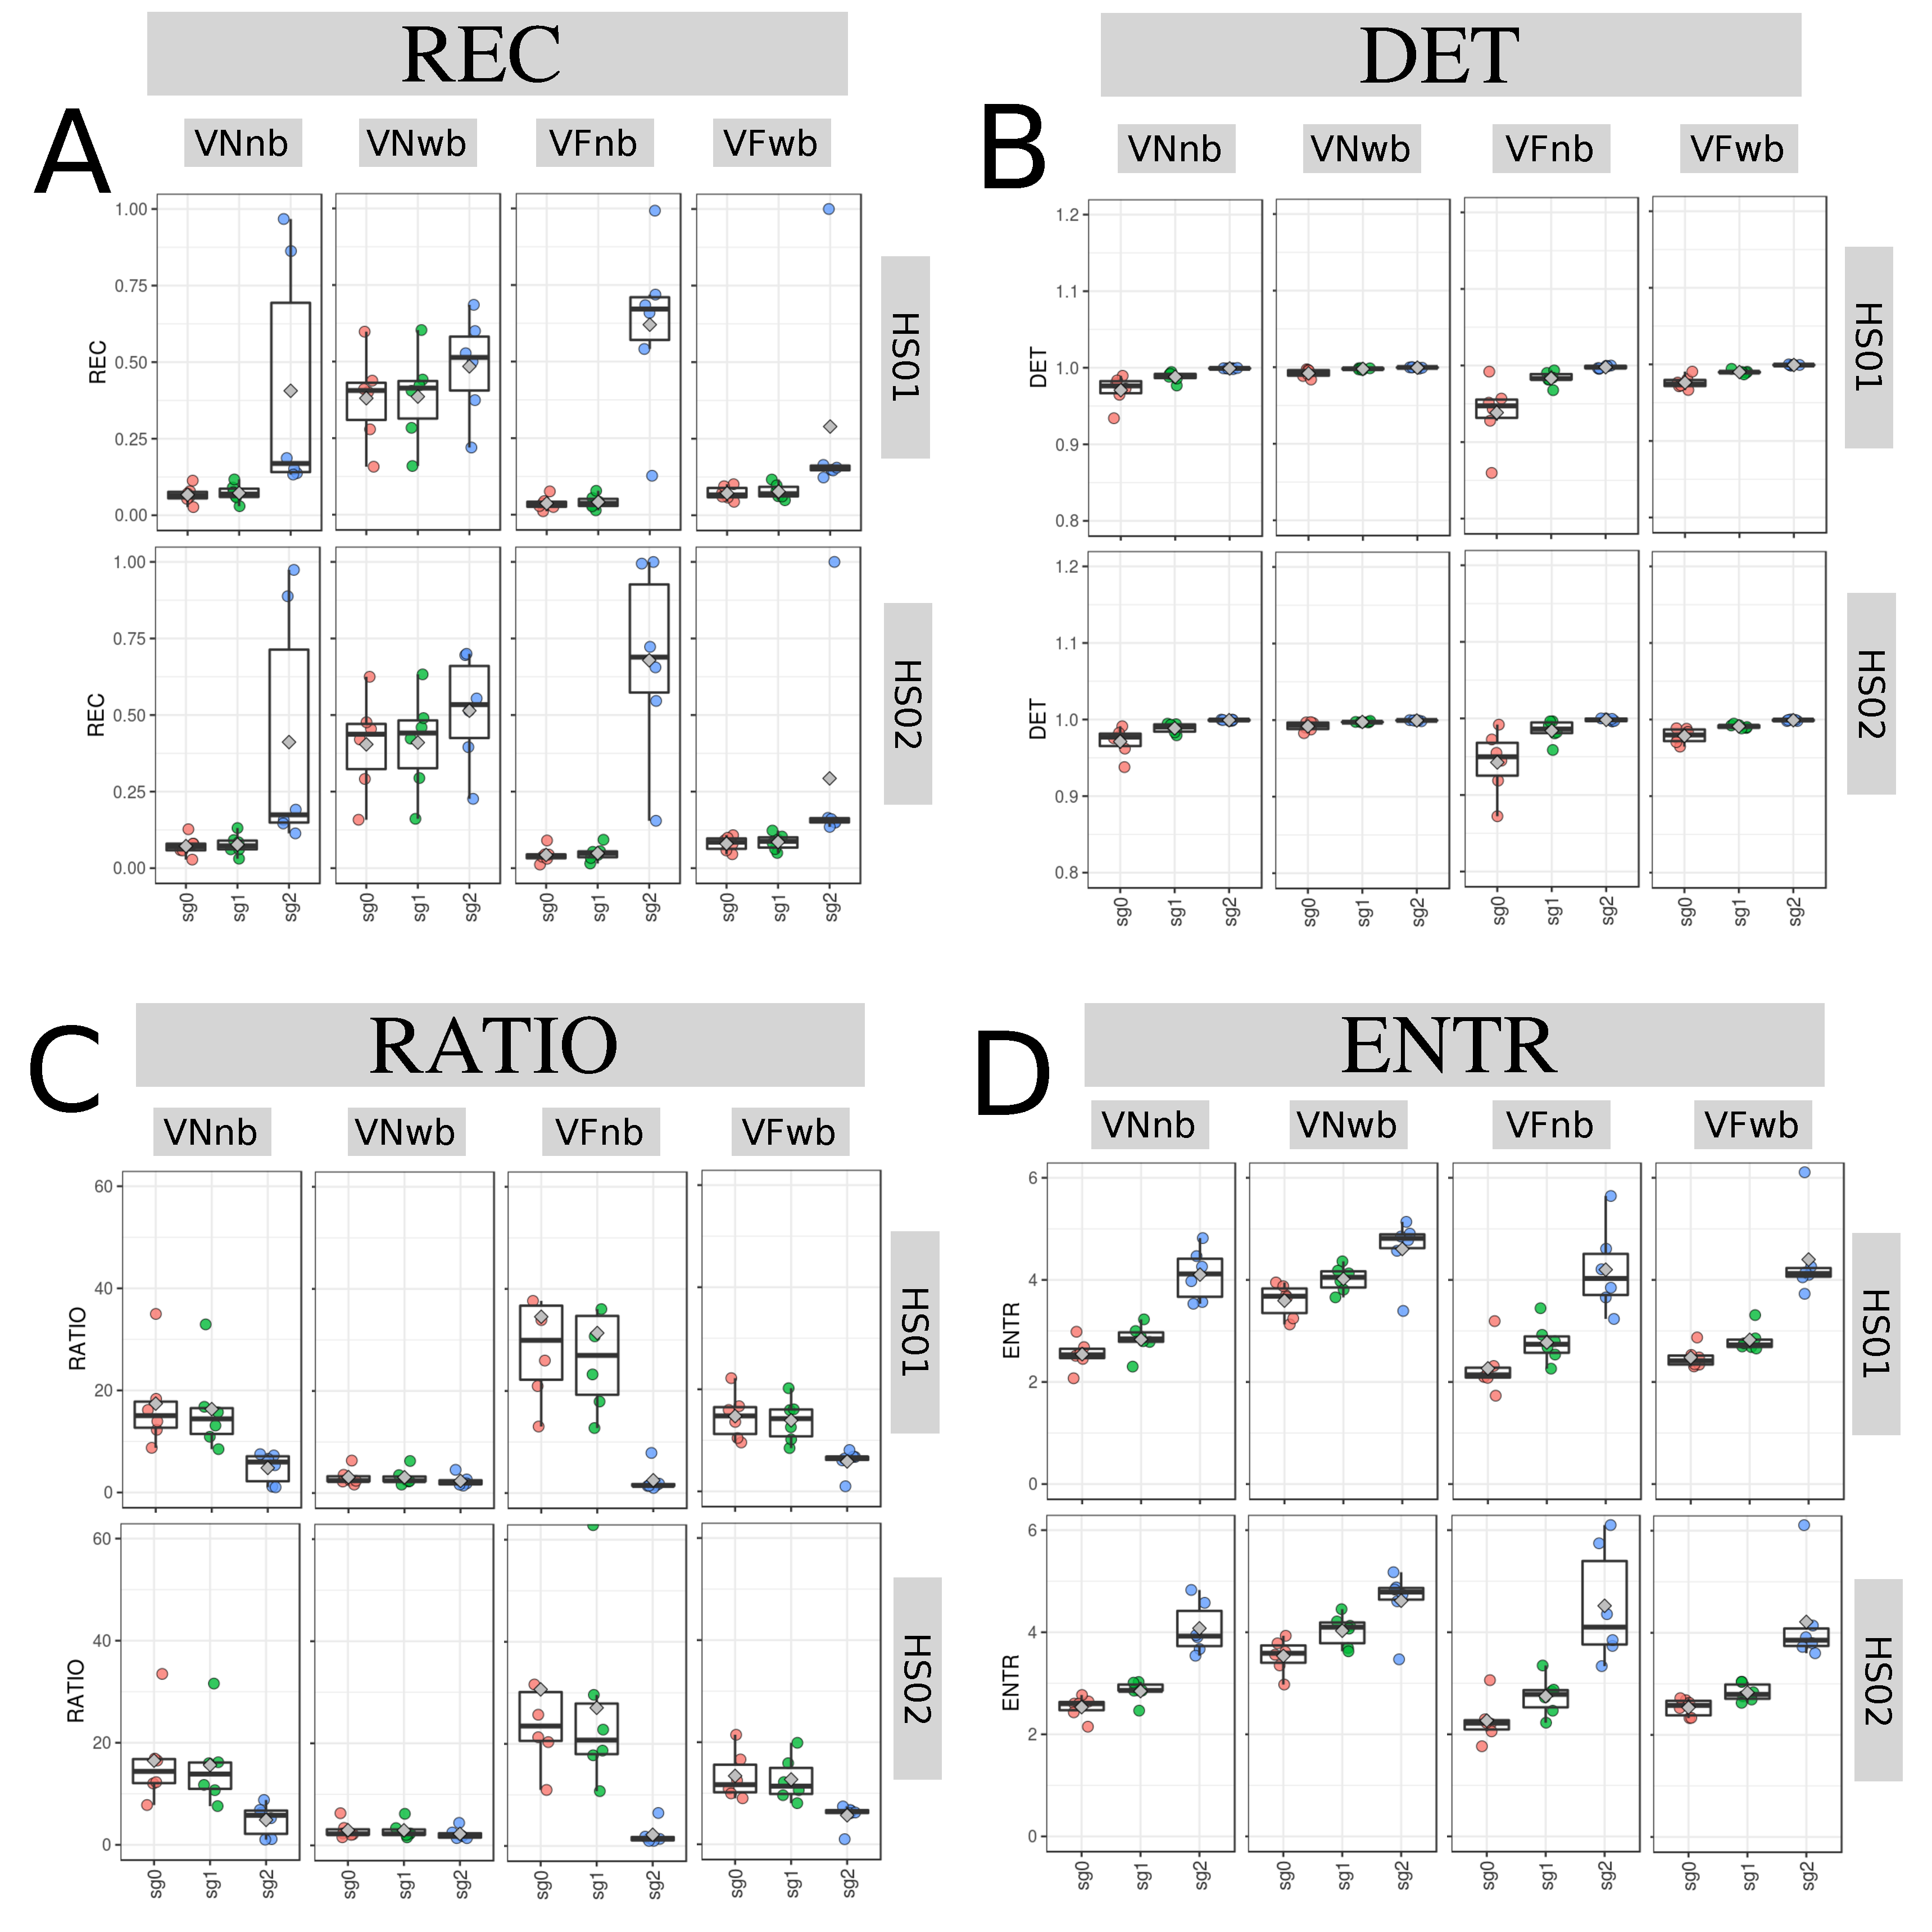
\includegraphics[width=1.0\textwidth]{fig_5_14}
	\caption
	[Box plots for RQA values for vertical arm movements]{
	{\bf Box plots for RQA values for vertical arm movements.} 
 	Box plots of (A) REC, (B) DET, (C) RATIO, and (D) ENTR values 
	for 6 participants performing VNnb, VNwb, VFnb and VFwb movements
	with sensors HS01, HS02 and three smoothed-normalised  
	time series (sg0, sg1 and sg2).
	RQA values were computed with 
	embedding parameters $\overline{m_0}=6$, $\overline{\tau_0}=10$ and 
	recurrence threshold $\epsilon=1$.
	\R code to reproduce the figure is available at 
	\codelink{
	https://github.com/mxochicale-phd/thesis/tree/master/0_code_data/1_code/7_figs_ch5/06_fig5.13-5.14/code
	}.
        }
    \label{fig:BPRQAV}
\end{figure}
%%---------------------------------(FIGURE)-------------------------------------

\newpage
\section{Weaknesses and strengths of RQA} \label{wsRQAhii}
Surfaces for RQA metrics (REC, DET, RATIO, ENTR) are computed with the 
variation of embedding values by an increase of one 
($0 \ge m \le 10$, $0 \ge \tau \le 10$) 
and recurrence thresholds by an increase of 0.1 ($0.2 \ge \epsilon \le 3$).
Hence, different characteristics of 3D surface plots of RQA 
are shown by considering different activities, sensors, 
window lengths and level of smoothness and participants.

Figs \ref{fig:topo_rqas_w500} show the 3D surface plots for RQA metrics 
(REC, DET, RATIO, ENTR) using time series of participant $p01$, 
sensor HS01, activity HNnb, sg0zmuvGyroZ axis and a 10 
seconds window length.
The 3D surface plot of REC values, representing the \% of recurrence dots 
in the RP, show highest values of REC when embedding values 
are near to 1 and the recurrence threshold is at the maximum 
($\epsilon = 3$ for this surface plot). Similarly, it can be seen a decrease
of REC values as the embedding dimension and embedding delay values 
increase, however there is an increase of REC values as the recurrence 
threshold is increasing (Fig \ref{fig:topo_rqas_w500}(A)).
Regarding the 3D surface plots of DET values, representing predictability 
and organisation of the RPs, Fig \ref{fig:topo_rqas_w500}(B) show slightly 
uniform values when varying both embedding parameters and recurrence 
threshold with the exception of embedding parameters near to 1 and 
recurrence thresholds near to 0.2 where the DET values are smaller.
3D surface for RATIO values, representing dynamic transitions, show 
a plateau with low values recurrence threshold values greater than 1.0.
However, there is a fluctuated increase of RATIO values as the embedding 
values increase given that the recurrence threshold is lower 
than 1 (Fig \ref{fig:topo_rqas_w500}(C)).
For ENTR values, representing the complexity of the structure of the 
time series, Fig \ref{fig:topo_rqas_w500}(D) show a maximum value of 
ENTR when embedding parameters are near to 1 and recurrence threshold values
are near to 3.0. It can also be noted fluctuations in the 3D surface 
when ENTR values are greater than 2.5 (red surface) for embedding 
dimensions between 3 to 9 and a decrease of ENTR values per each 
embedding dimension for delay embedding values (yellow surface).
Additionally, ENTR values decrease as the embedding dimension and 
delay embedding decrease.
%%---------------------------------(FIGURE)-----------------------------------
\begin{figure}[h!]
\centering
\includegraphics[width=1.0\textwidth]{fig_5_15}
    \caption
	[3D surface plots of RQA metrics]{
	{\bf 3D surface plots of RQA metrics.}
	3D surface plots of RQA metrics (A) REC, (B) DET, (C) RATIO and 
	(D) ENTR with an increasing pair of embedding parameters 
	($0 \le m_0 \le 10$, $0 \le \tau_0 \le 10$) 
	and recurrence thresholds ($ 0.2 \le \epsilon_r \le 3 $).
	RQA metrics are computed with the time series of participant $p01$ using 
	HS01 sensor, HNnb activity, sg0zmuvGyroZ axis and 10 seconds 
	for window length.
	\R code to reproduce the figure is available at 
	\codelink{
	https://github.com/mxochicale-phd/thesis/tree/master/0_code_data/1_code/7_figs_ch5/07_fig5.15/code
	}.
	}
\label{fig:topo_rqas_w500}
\end{figure}
%%---------------------------------(FIGURE)------------------------------------

\newpage
\subsection{Sensors and activities}
Figs \ref{fig:topo_s_hs01_H_w500} and \ref{fig:topo_s_hs02_H_w500} show
3D surface plots of RQA metrics (REC, DET, RATIO, ENTR) for horizontal arm 
movements (HNnb, HNwb, HFnb, HFwb) using sensor HS01 and HS02 
for participant $p01$ with sg0zmuvGyroZ axis and 10 seconds window length.
Hence, Figs \ref{fig:topo_s_hs01_H_w500} present 3D surface plots of RQA metrics 
for HS01, where 3D surface plots of REC values 
(Fig \ref{fig:topo_s_hs01_H_w500}(A)) appear to be similar across 
the activities (HNnb, HFnb, HFwb) with the exception of HNwb which 
decrease of REC values is mainly affected by the increase of recurrence 
threshold and slightly affected to the increase of embedding dimension 
parameters. For DET values, 3D surface plots in Figs \ref{fig:topo_s_hs01_H_w500}(B)
appear to show values near to 1.0 (red colour surface), however HNwb 
shown fluctuations of DET values as the embedding dimension increase, 
it can also be noted a decrease of DET values for certain values of 
recurrence threshold (2.6 for HNwb, 0.3 for HFnb, and 0.3 for HFwb).
For Fig \ref{fig:topo_s_hs01_H_w500}(C)), 3D surface plots of RATIO values 
appear to be similar, showing a plateau for values between 0 to 50 
(blue surface) and the increase of peaks is different for each of the 
activities.
For Fig \ref{fig:topo_s_hs01_H_w500}(D), ENTR values present different 
surface formations, for instance, 
HNnb show fluctuated higher values of ENTR (red colour surface),
whereas for activity HNwb the ENTR values are higher (red colour surface) 
for recurrence threshold near to 3.0,
ENTR values for HFnb appear to be higher when embedding dimension is near 
to 10, while higher values for ENTR values for HFwb appear to be 
when the recurrence threshold is near to 0.2.

Then, looking and comparing visually one by one of the 3D surface plots 
for sensors HS01 and HS02 in Figs \ref{fig:topo_s_hs01_H_w500} 
and \ref{fig:topo_s_hs02_H_w500}, one can notice little differences in the 
shape of the surface plots.
Similarly, there is little variations in the surface plots for vertical arm 
movements with the sensors HS01 and HS02 
(Figs \ref{fig:topo_s_hs01_V_w500} and \ref{fig:topo_s_hs02_V_w500}).

With regards to horizontal and vertical movements, 
3D surface plots appear to be similar for REC, DET and RATIO values
with sensor HS01
(Figs \ref{fig:topo_s_hs01_H_w500} and \ref{fig:topo_s_hs01_V_w500})
and sensor HS02
(Figs \ref{fig:topo_s_hs02_H_w500} and \ref{fig:topo_s_hs02_V_w500}), 
however 3D surface plots of ENTR values in each of the arm movements
presents distinguishable variations in the surface plots,
see Figs \ref{fig:topo_s_hs01_H_w500}(D) and \ref{fig:topo_s_hs01_V_w500}(D) 
for horizontal and vertical arm movements with sensor HS01 and
Figs \ref{fig:topo_s_hs02_H_w500}(D) and \ref{fig:topo_s_hs02_V_w500}(D) 
for horizontal and vertical arm movements with sensor HS02.

%%---------------------------------(FIGURE)------------------------------------
\begin{figure}
\centering
\includegraphics[width=1.0\textwidth]{fig_5_16}
    \caption
	[3D surface plots of RQA metrics for horizontal arm movements with HS01]{
	{\bf 3D surface plots of RQA metrics for horizontal arm movements with HS01.}
	3D surface plots for (A) REC, (B) DET, (C) RATIO and (D) ENTR values 
	with increasing pair of embedding parameters 
	($0 \le m \le 10$, $0 \le \tau \le 10$) 
	and recurrence thresholds ($ 0.2 \le \epsilon \le 3 $).
	RQA metrics are computed with the time series of participant $p01$ 
	for sensors HS01, horizontal arm movement activities 
	(HNnb, HNwb, HFnb, HFwb) and 
	sg0zmuvGyroZ axis with 10 seconds window length. 
	\R code to reproduce the figure is available at 
	\codelink{
	https://github.com/mxochicale-phd/thesis/tree/master/0_code_data/1_code/7_figs_ch5/08_fig5.16-5.17-5.18-5.19/code	
	}.
	}
\label{fig:topo_s_hs01_H_w500}
\end{figure}
%%---------------------------------(FIGURE)------------------------------------

%%---------------------------------(FIGURE)------------------------------------
\begin{figure}
\centering
\includegraphics[width=1.0\textwidth]{fig_5_17}
    \caption
	[3D surface plots of RQA metrics for horizontal arm movements with HS02]{
	{\bf 3D surface plots of RQA metrics for horizontal arm movements with HS02.}
	3D surface plots for (A) REC, (B) DET, (C) RATIO and (D) ENTR values 
	with increasing pair of embedding parameters 
	($0 \le m \le 10$, $0 \le \tau \le 10$) 
	and recurrence thresholds ($ 0.2 \le \epsilon \le 3 $).
	RQA metrics are computed with the time series of participant $p01$ 
	for sensors HS02, horizontal arm movement activities 
	(HNnb, HNwb, HFnb, HFwb) and 
	sg0zmuvGyroZ axis with 10 seconds window length. 
 	\R code to reproduce the figure is available at 
	\codelink{
	https://github.com/mxochicale-phd/thesis/tree/master/0_code_data/1_code/7_figs_ch5/08_fig5.16-5.17-5.18-5.19/code	
	}.
	}
\label{fig:topo_s_hs02_H_w500}
\end{figure}
%%---------------------------------(FIGURE)------------------------------------

%%---------------------------------(FIGURE)-----------------------------------
\begin{figure}
\centering
\includegraphics[width=1.0\textwidth]{fig_5_18}
    \caption
	[3D surface plots of RQA metrics for vertical arm movements with HS01]{
	{\bf 3D surface plots of RQA metrics for vertical arm movements with HS01.}
	3D surface plots for (A) REC, (B) DET, (C) RATIO and (D) ENTR values 
	with increasing pair of embedding parameters 
	($0 \le m \le 10$, $0 \le \tau \le 10$) 
	and recurrence thresholds ($ 0.2 \le \epsilon \le 3 $).
	RQA metrics are computed with the time series of participant $p01$ 
	for sensors HS01, vertical arm movements activities 
	(VNnb, VNwb, VFnb, VFwb) and 
	sg0zmuvGyroY axis with 10 seconds window length. 
 	\R code to reproduce the figure is available at 
	\codelink{
	https://github.com/mxochicale-phd/thesis/tree/master/0_code_data/1_code/7_figs_ch5/08_fig5.16-5.17-5.18-5.19/code	
	}.
	}
\label{fig:topo_s_hs01_V_w500}
\end{figure}
%%---------------------------------(FIGURE)------------------------------------


%%---------------------------------(FIGURE)------------------------------------
\begin{figure}
\centering
\includegraphics[width=1.0\textwidth]{fig_5_19}
    \caption
	[3D surface plots of RQA metrics for vertical arm movements with HS02]{
	{\bf 3D surface plots of RQA metrics for vertical arm movements with HS02.}
	3D surface plots for (A) REC, (B) DET, (C) RATIO and (D) ENTR values 
	with increasing pair of embedding parameters 
	($0 \le m \le 10$, $0 \le \tau \le 10$) 
	and recurrence thresholds ($ 0.2 \le \epsilon \le 3 $).
	RQA metrics are computed with the time series of participant $p01$ 
	for sensors HS02, vertical arm movements activities 
	(VNnb, VNwb, VFnb, VFwb) and 
	sg0zmuvGyroY axis with 10 seconds window length. 
 	\R code to reproduce the figure is available at 
	\codelink{
	https://github.com/mxochicale-phd/thesis/tree/master/0_code_data/1_code/7_figs_ch5/08_fig5.16-5.17-5.18-5.19/code	
	}.
	}
\label{fig:topo_s_hs02_V_w500}
\end{figure}
%%---------------------------------(FIGURE)------------------------------------

\newpage
\subsection{Window size}
3D surface plots of REC values with a short window length (2-secs) 
can affect the shape of 3D surface, however for window size of 
5-sec, 10-sec and 15-sec, the 3D surface plots appear to show little changes 
(Figs \ref{fig:topo_windows_hii}(A)).
For instance, one can see 3D surface plots of DET values with a window of 
2 seconds window length is slightly different to other surface plots but 
keeping the plateau (red surface) in each of the surface plots
(Figs \ref{fig:topo_windows_hii}(B)).
Similarly, the 3D surface plots of RATIO values preserve the same plateau 
(blue surface) with little variations in the surface plots as window length 
is incrementing (Figs \ref{fig:topo_windows_hii}(C)).
3D surface plots of ENTR values appear to have similar aspects as the 
fluctuations of the curves keeps the same values (red and yellow colours).
It can also be noted that the smoothness of 3D surface plots decrease as the 
embedding dimension parameters increase and such smoothness is also affected 
by the window length (see Figs \ref{fig:topo_windows_hii}(D)).

%---------------------------------(FIGURE)-------------------------------------
\begin{figure}
\centering
\includegraphics[width=1.0\textwidth]{fig_5_20}
    \caption
	[3D surface plots of RQA metrics for different window lengths]{
	{\bf 3D surface plots of RQA metrics for different window lengths.}
	3D surface plots for four window lengths (w2-sec, w5-sec, w10-sec and  w15-sec)
	and for (A) REC, (B) DET, (C) RATIO, and (D) ENTR values
	with increasing pair of embedding parameters 
	($0 \le m \le 10$, $0 \le \tau \le 10$) 
	and recurrence thresholds ($ 0.2 \le \epsilon \le 3 $).
	RQA metrics are computed with the time series of participant $p01$ 
	using HS01 sensor, HNnb activity and sg0zmuvGyroZ axis.
	\R code to reproduce the figure is available at 
	\codelink{
	https://github.com/mxochicale-phd/thesis/tree/master/0_code_data/1_code/7_figs_ch5/09_fig5.20/code
	}.
       }
\label{fig:topo_windows_hii}
\end{figure}
%%---------------------------------(FIGURE)------------------------------------

\subsection{Smoothness}
Figs \ref{fig:topo_smoothness_hii} show the effects of three levels of 
smoothness (sg0zmuvGyroZ, sg1zmuvGyroZ and sg2zmuvGyroZ) in the RQA metrics.
Generally, 3D surface plots from sg2zmuvGyroZ are affected by the smoothness.
It can also be noted that REC values and ENTR values present a slightly 
different surface plots (see Figs \ref{fig:topo_smoothness_hii}(A, D)), 
while DET and RATIO values appear to be similar which is mainly reflected in 
the colour of the curves (see Figs \ref{fig:topo_smoothness_hii}(B, C)).
In Figs \ref{fig:topo_smoothness_hii}(A), 3D surface plots for REC values tend be 
smoothed as the smoothness of the time series increase to the point where 
the increase of recurrence threshold affects the shape of the surface plots.
Similarly, in Figs  \ref{fig:topo_smoothness_hii}(D), 
3D surface for ENTR values is affected by the smoothness of the 
time series to the point that the fluctuations in the surface does change 
drastically the shape by showing only an increase of ENTR values as
the recurrence threshold increase.

%%---------------------------------(FIGURE)------------------------------------
\begin{figure}
\centering
\includegraphics[width=0.9\textwidth]{fig_5_21}
    \caption
	[3D surface plots of RQA metrics with three levels of smoothness]{
	{\bf 3D surface plots of RQA metrics with three levels of smoothness.}
	3D surface plots for 
	three levels of smoothness (sg0zmuvGyroZ, sg1zmuvGyroZ, and sg2zmuvGyroZ) 
	and for (A) REC, (B) DET, (C) RATIO, and (D) ENTR values 
	with increasing pair of embedding parameters 
	($0 \le m \le 10$, $0 \le \tau \le 10$) 
	and recurrence thresholds ($ 0.2 \le \epsilon \le 3 $).
	RQA metrics are computed with the time series of participant $p01$ with
	HS01 sensor, HNnb activity and 10 seconds window length.
	\R code to reproduce the figure is available at 
	\codelink{
	https://github.com/mxochicale-phd/thesis/tree/master/0_code_data/1_code/7_figs_ch5/10_fig5.21/code
	}.
 }
\label{fig:topo_smoothness_hii}
\end{figure}
%%---------------------------------(FIGURE)------------------------------------

\newpage
\subsection{Participants}
The shape of 3D surface plots of RQA metrics is also affected when using 
time series from different participants (Figs \ref{fig:topo_participants_hii}).
For instance, 3D surface of DET values show slightly but noticeable 
differences in the fluctuations when embedding dimension and recurrence 
threshold increase (Figs \ref{fig:topo_participants_hii}(B)) which is similar 
for ENTR values where the fluctuations of the 3D surface plots changes for each 
of the participants (Figs \ref{fig:topo_participants_hii}(D)).
However, the shape of 3D surface plots for RET values and RATIO values 
is little affected by the change of participants 
(Figs \ref{fig:topo_participants_hii}(A, C)).

%%---------------------------------(FIGURE)------------------------------------
\begin{figure}
\centering
\includegraphics[width=1.0\textwidth]{fig_5_22}
    \caption
	[3D surface plots of RQA metrics with four participants]{
	{\bf 3D surface plots of RQA metrics with four participants.}
	3D surface plots for participants $p01$, $p04$, $p05$ and $p10$
	and for (A) REC, (B) DET, (C) RATIO, and (D) ENTR 
	with increasing pair of embedding parameters 
	($0 \le m \le 10$, $0 \le \tau \le 10$) 
	and recurrence thresholds ($ 0.2 \le \epsilon \le 3 $).
	RQA metrics are computed with the time series of
	sg0zmuvGyroZ axis, HS01 sensor, HNnb activity and 
	10 seconds window length.
	\R code to reproduce the figure is available at 
	\codelink{
	https://github.com/mxochicale-phd/thesis/tree/master/0_code_data/1_code/7_figs_ch5/11_fig5.22/code
	}.
 }
\label{fig:topo_participants_hii}
\end{figure}
%%---------------------------------(FIGURE)-------------------------------------

\newpage
\subsection{Final remarks}
Different sources of time series (participants, sensors, 
activities, window length or level of smoothness) produce different
results in nonlinear analysis methods 
(e.g. FNN, AMI, RSSs with UTDE, RPs and RQAs) 
and these results are sensitive 
to different parameters of nonlinear analysis
methods (e.g., minimum dimension threshold, 
embedding parameters or recurrence thresholds).
That said, 3D surface plots of RQA metrics with the 
variation of embedding parameters and recurrence thresholds
appear to be helpful to understand the dynamics of 
any type of time series data.
That is the case of 3D surface plots of ENTR values which with 
only the selection of variation of range of parameters
(e.g., embedding parameters or recurrence thresholds),
the 3D surface plots show clearly differences in the shape 
of 3D surface plots irregardless of the source of the time series. 
Hence, computing 3D surface plots of ENTR values
with little parametrisation might be of help to understand 
the dynamics of human movement variability from different
sources of time series data.

 %Quantifying Human Imitation Activities
%*******************************************************************************
%****************************** Sixth Chapter *********************************
%*******************************************************************************

\chapter{Quantifying Human-Humanoid Imitation Activities} \label{chapter6}

%% **************************** Define Graphics Path **************************
%\ifpdf
%    \graphicspath{{chapter7/figs/raster/}{chapter7/figs/PDF/}{chapter7/figs/}}
%\else
%    \graphicspath{{chapter7/figs/vector/}{chapter7/figs/}}
%\fi
\graphicspath{{figs/chapter6/PDF/}}

\section{Introduction} 
Considering the experiment of Human-Humanoid Imitation Activities
(Section \ref{sec:experiment:hhi}), 
we investigated the robustness and weaknesses of the reconstructed 
state spaces (RSSs) using the uniform time-delay embedding technique (UTDE) 
and recurrence plots (RPs) for recurrent quantification analysis (RQA) 
methodologies for the following conditions of time series data: 
\begin{itemize}

\item Three levels of smoothness for the normalised data 
(sg0zmuv, sg1zmuv and sg2zmuv), computed from two different filter 
lengths (29 and 159) with the same polynomial degree of 5 using the 
function \texttt{sgolay(p,n,m)} \citep{Rsignal},

\item Four velocities of arm movement activity: horizontal normal (HN), 
	horizontal faster (HF), vertical normal (VN) and 
	vertical faster (VF), and
\item Four window length size: 2-sec (100 samples), 5-sec (250 samples), 
	10-sec (500 samples) and 15-sec (750 samples).
\end{itemize}

Further details about the processing of time series are presented in
Section \ref{sec:preparation_timeseries}.

\section{Time series}
To make visual comparison easier, we only present a 10-sec (500 samples) 
window length time series for three participants ($p01$, $p02$ and $p03$) 
performing horizontal 
arm movements using axis GyroZ (Figs. \ref{fig:tsH})
and  vertical arm movements using axis GyroY (Figs. \ref{fig:tsV}). 
Other data are presented in Appendix \ref{appendix:d}.
We consider different levels of smoothness of the normalised data 
with two different Savitzky-Golay filter lengths (29 and 159) 
with the same polynomial degree of 5 using \texttt{sgolay(p,n,m)} 
\citep{Rsignal}. 
%%---------------------------------(FIGURE)-------------------------------------
\begin{figure}[!h]
  \centering
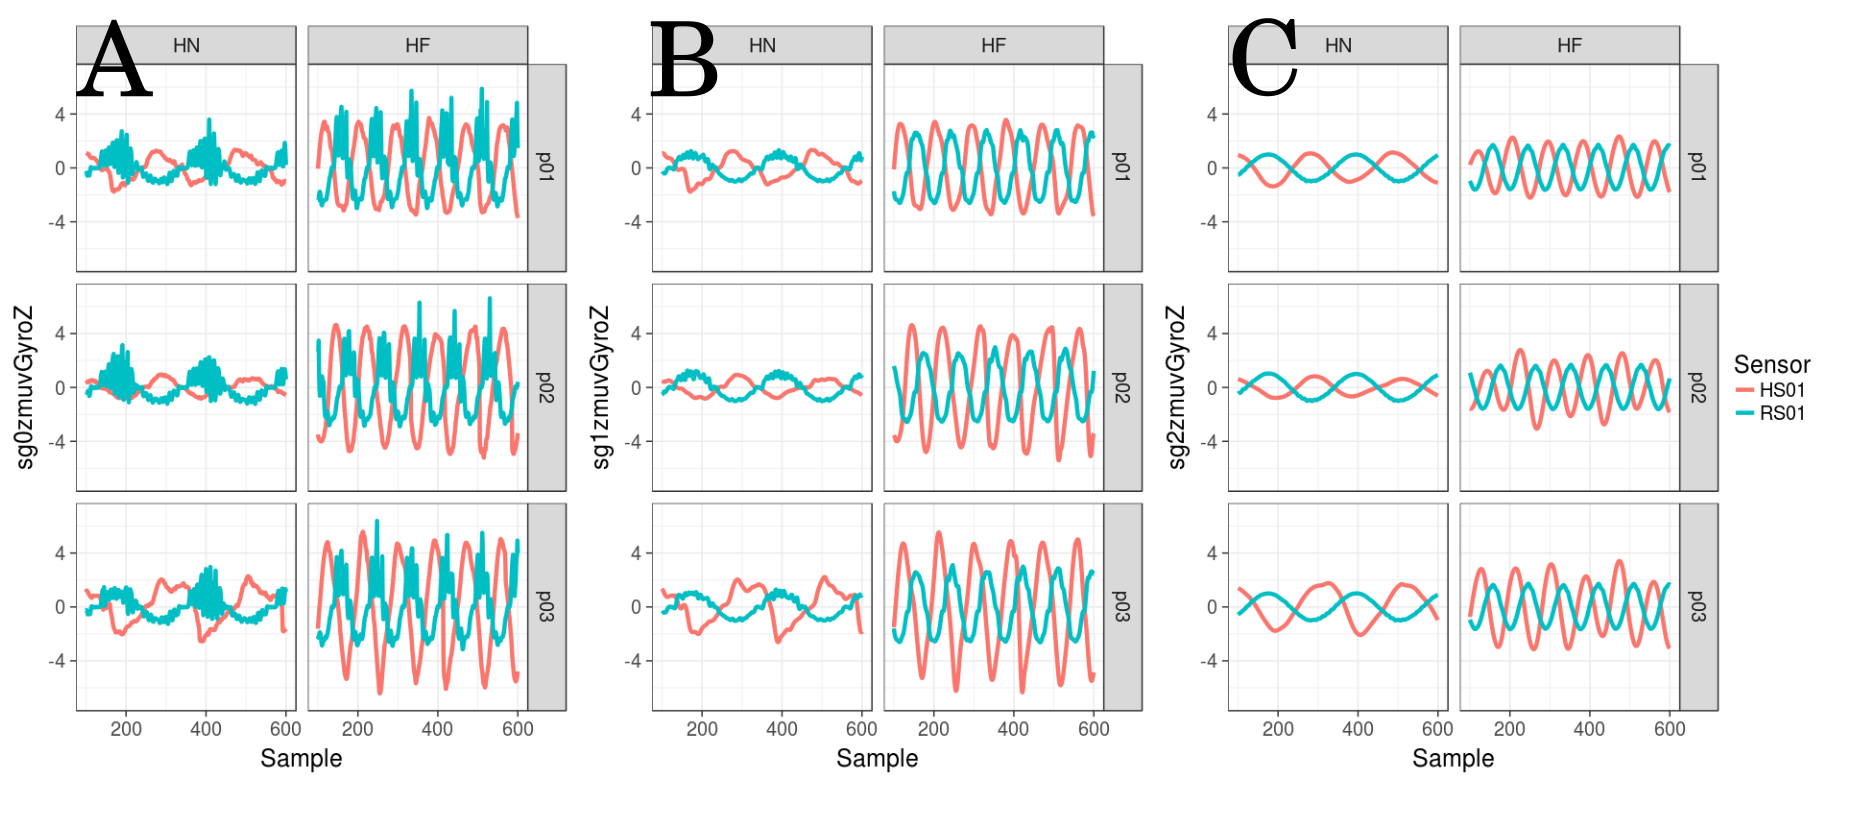
\includegraphics[width=1.0\textwidth]{tsHv03}
    	\caption
	[Time series for horizontal arm movements]{
	{\bf Time series for horizontal arm movements.}
		(A) raw-normalised (sg0zmuvGyroZ), 
		(B) normalised-smoothed 1 (sg1zmuvGyroZ) and
		(C) normalised-smoothed 2 (sg2zmuvGyroZ).
		Time series are only for three participants 
		($p01$, $p02$, and $p03$) 
		for horizontal movements in normal and faster velocity (HN, HF) 
		with the normalised GyroZ axis (zmuvGyroZ) 
		and with one sensor attached to the participant (HS01) 
		and other sensor attached to the robot (RS01).	
	R code to reproduce the figure is available from \cite{hwum2018}.
        }
    \label{fig:tsH}
\end{figure}
%%---------------------------------(FIGURE)------------------------------------
%%---------------------------------(FIGURE)-------------------------------------
\begin{figure}[!h]
  \centering
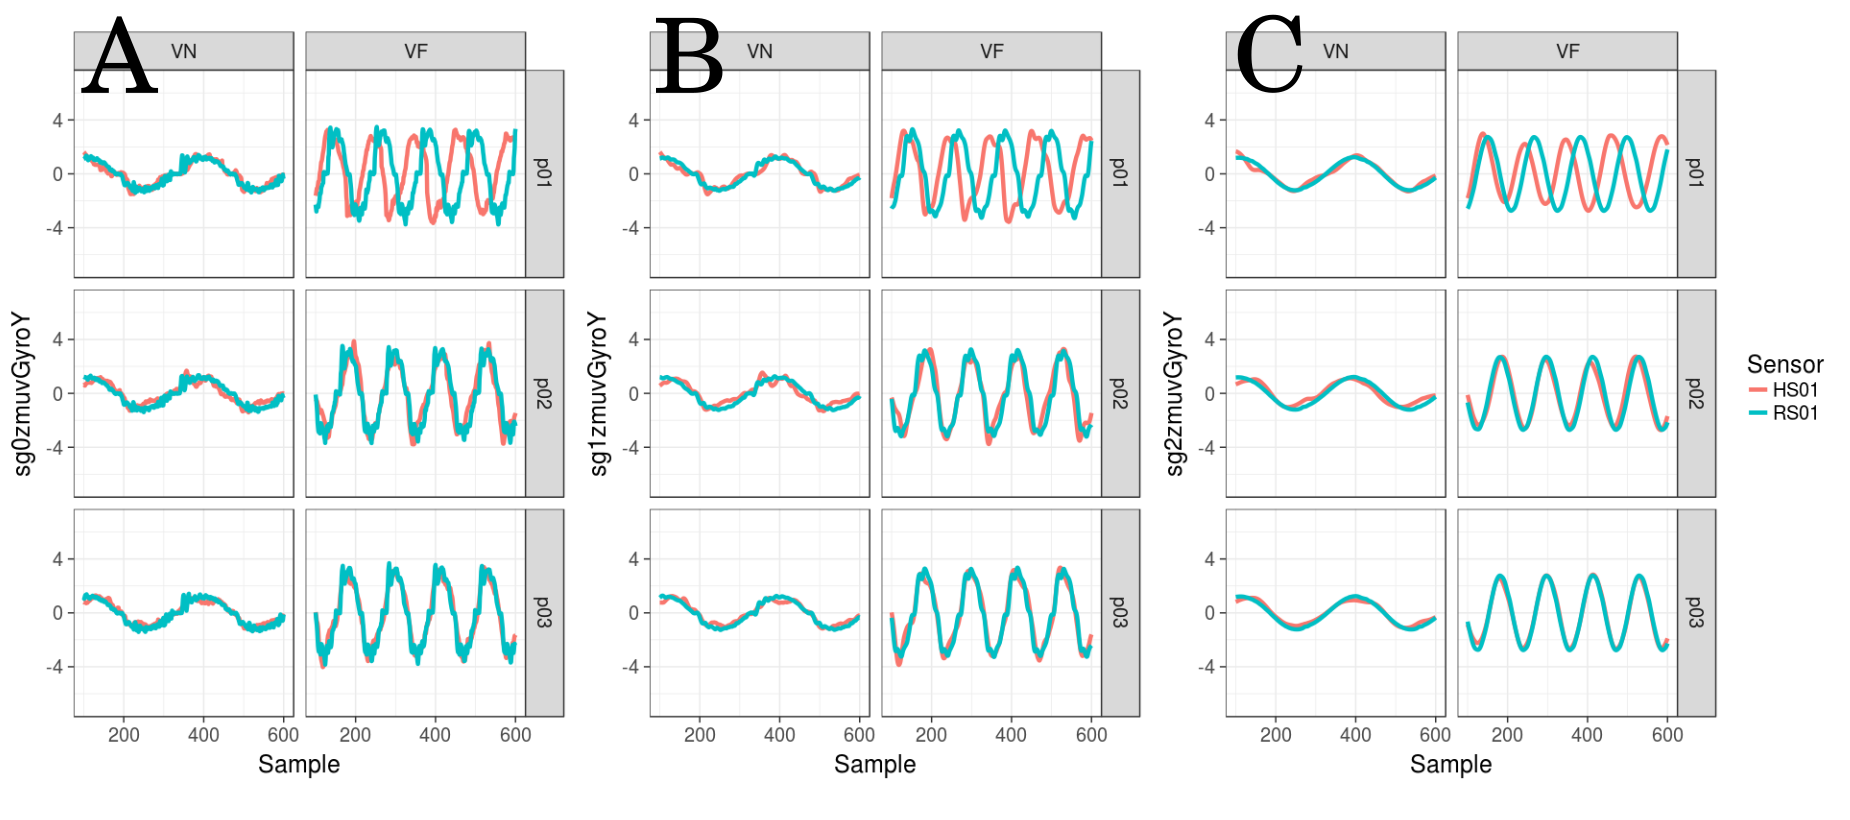
\includegraphics[width=1.0\textwidth]{tsVv03}
	\caption
	[Time series for vertical arm movements]{
	{\bf Time series for vertical arm movements.}
		(A) raw-normalised (sg0zmuvGyroY), 
		(B) normalised-smoothed 1 (sg1zmuvGyroY) and
		(C) normalised-smoothed 2 (sg2zmuvGyroY).
		Time series are only for three participants 
		($p01$, $p02$, and $p03$) 
		for vertical movements in normal and faster velocity (VN, VF) 
		with the normalised GyroY axis (zmuvGyroY) 
		and with one sensor attached to the participant (HS01) 
		and other sensor attached to the robot (RS01).
		R code to reproduce the figure is available 
		from \cite{hwum2018}.
        }
    \label{fig:tsV}
\end{figure}
%%---------------------------------(FIGURE)------------------------------------







\section{Minimum Embedding Parameters}
As mentioned in Section \ref{mep-hii} in Chapter \ref{chapter5}, 
we computed minimum embedding parameters using FNN and AMI algorithms
for time series of this section.

Hence, Figs \ref{fig:CAOAMI-hhi}(A) show box plots of the minimum embedding 
dimensions of twenty participants performing horizontal and vertical arm
movements at normal and faster velocities (HN, HF, VN and VF) with 
attached sensors to participants (HS01) and to the robot (RS01).
Generally, Figs \ref{fig:CAOAMI-hhi}(A) show that minimum embedding values 
appear to be constant for sensor RS01 as their interquartile range 
in the box plots are near to 0.1 with the exception of two axis. 
Minimum embedding values for sensor HS01 appear to show more variations 
as their interquartile range of the box plots are near to 1 
with four exceptions.
Additionally, it can be seen in Figs \ref{fig:CAOAMI-hhi}(A) that there is a 
decrease of mean values (rhombus) in the box plots
as smoothness of time series increase. 
See Figs. \ref{fig:caoH} and \ref{fig:caoV} in appendix \ref{appendix:e:ep} 
for detailed values of embedding dimensions for each participant.

Similarly, the first minimum values of AMI values 
for participants ($p01$ to $p20$), activities (HN, HF, VN, and VF) and 
sensors (HS01, RS01) are shown in the box plots of 
Figs \ref{fig:CAOAMI-hhi}(B).
It can be seen that values for HS01 tend to be more spread as the smoothness 
of the time series is increasing 
(see the increase of both mean (rhombus) and interquartile range).
However, AMI values for RS01 do not show such increase in relation with
the increase of smoothness excepting for HF and VF
(see the increase of both mean (rhombus) and interquartile range) 
(Figs \ref{fig:CAOAMI-hhi}(B)).
See Figs. \ref{fig:amiH} and \ref{fig:amiV} in appendix \ref{appendix:e:ep} 
for more details about AMI values for each participant.
%%---------------------------------(FIGURE)-------------------------------------
\begin{figure}
\centering
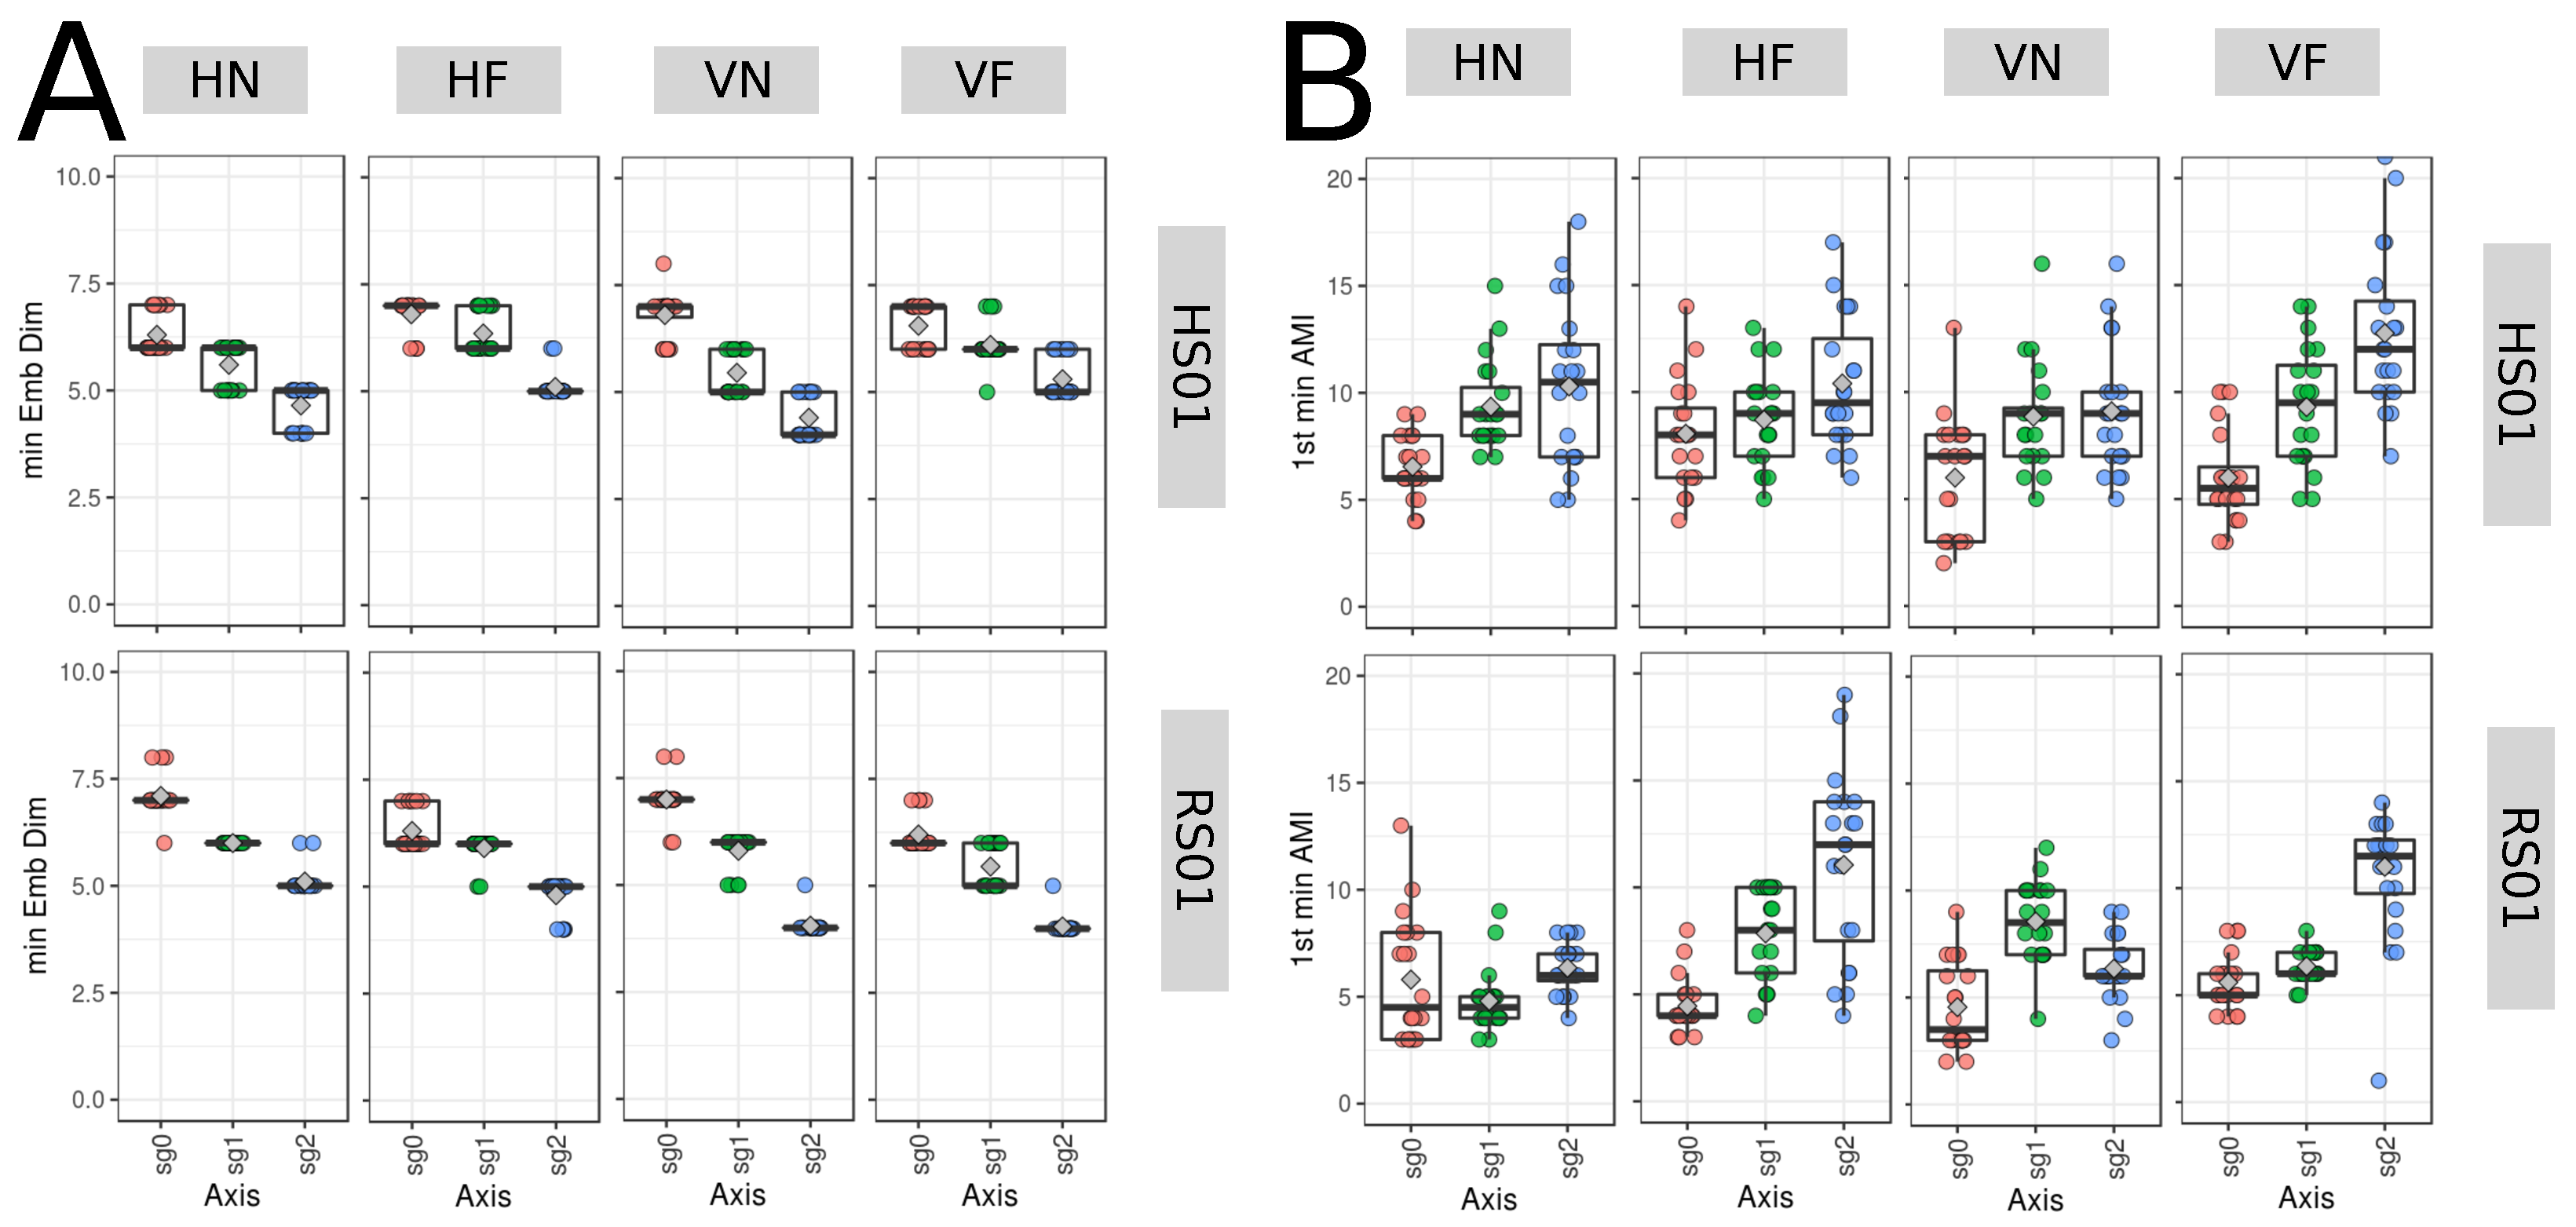
\includegraphics[width=1.0\textwidth]{CAOAMI}
	\caption
	[Box plots of minimum embedding parameters]{
	{\bf Box plots of minimum embedding parameters.} 
		Box plots of (A) minimum embedding dimensions 
		and (B) first minimum AMI values for 
		Horizontal Normal (HN), Horizontal Faster (HF),
		Vertical Normal (VN) and Vertical Faster (VF)
		with sensors attached to participants (HS01) and
		sensor attached to robot (RS01).
		Minimum embedding dimensions are for twenty participants 
		($p01$ to $p20$) with three smoothed signals 
		(sg0zmuvGyroZ (sg0) , sg1zmuvGyroZ (sg1) and sg2zmuvGyroZ (sg2))
		and window length of 10-sec (500 samples).
		R code to reproduce the figure is available 
		from \cite{hwum2018}.
        }
    \label{fig:CAOAMI-hhi}
\end{figure}
%%---------------------------------(FIGURE)------------------------------------




%%%---------------------------------(FIGURE)-------------------------------------
%\begin{figure}
%\centering
%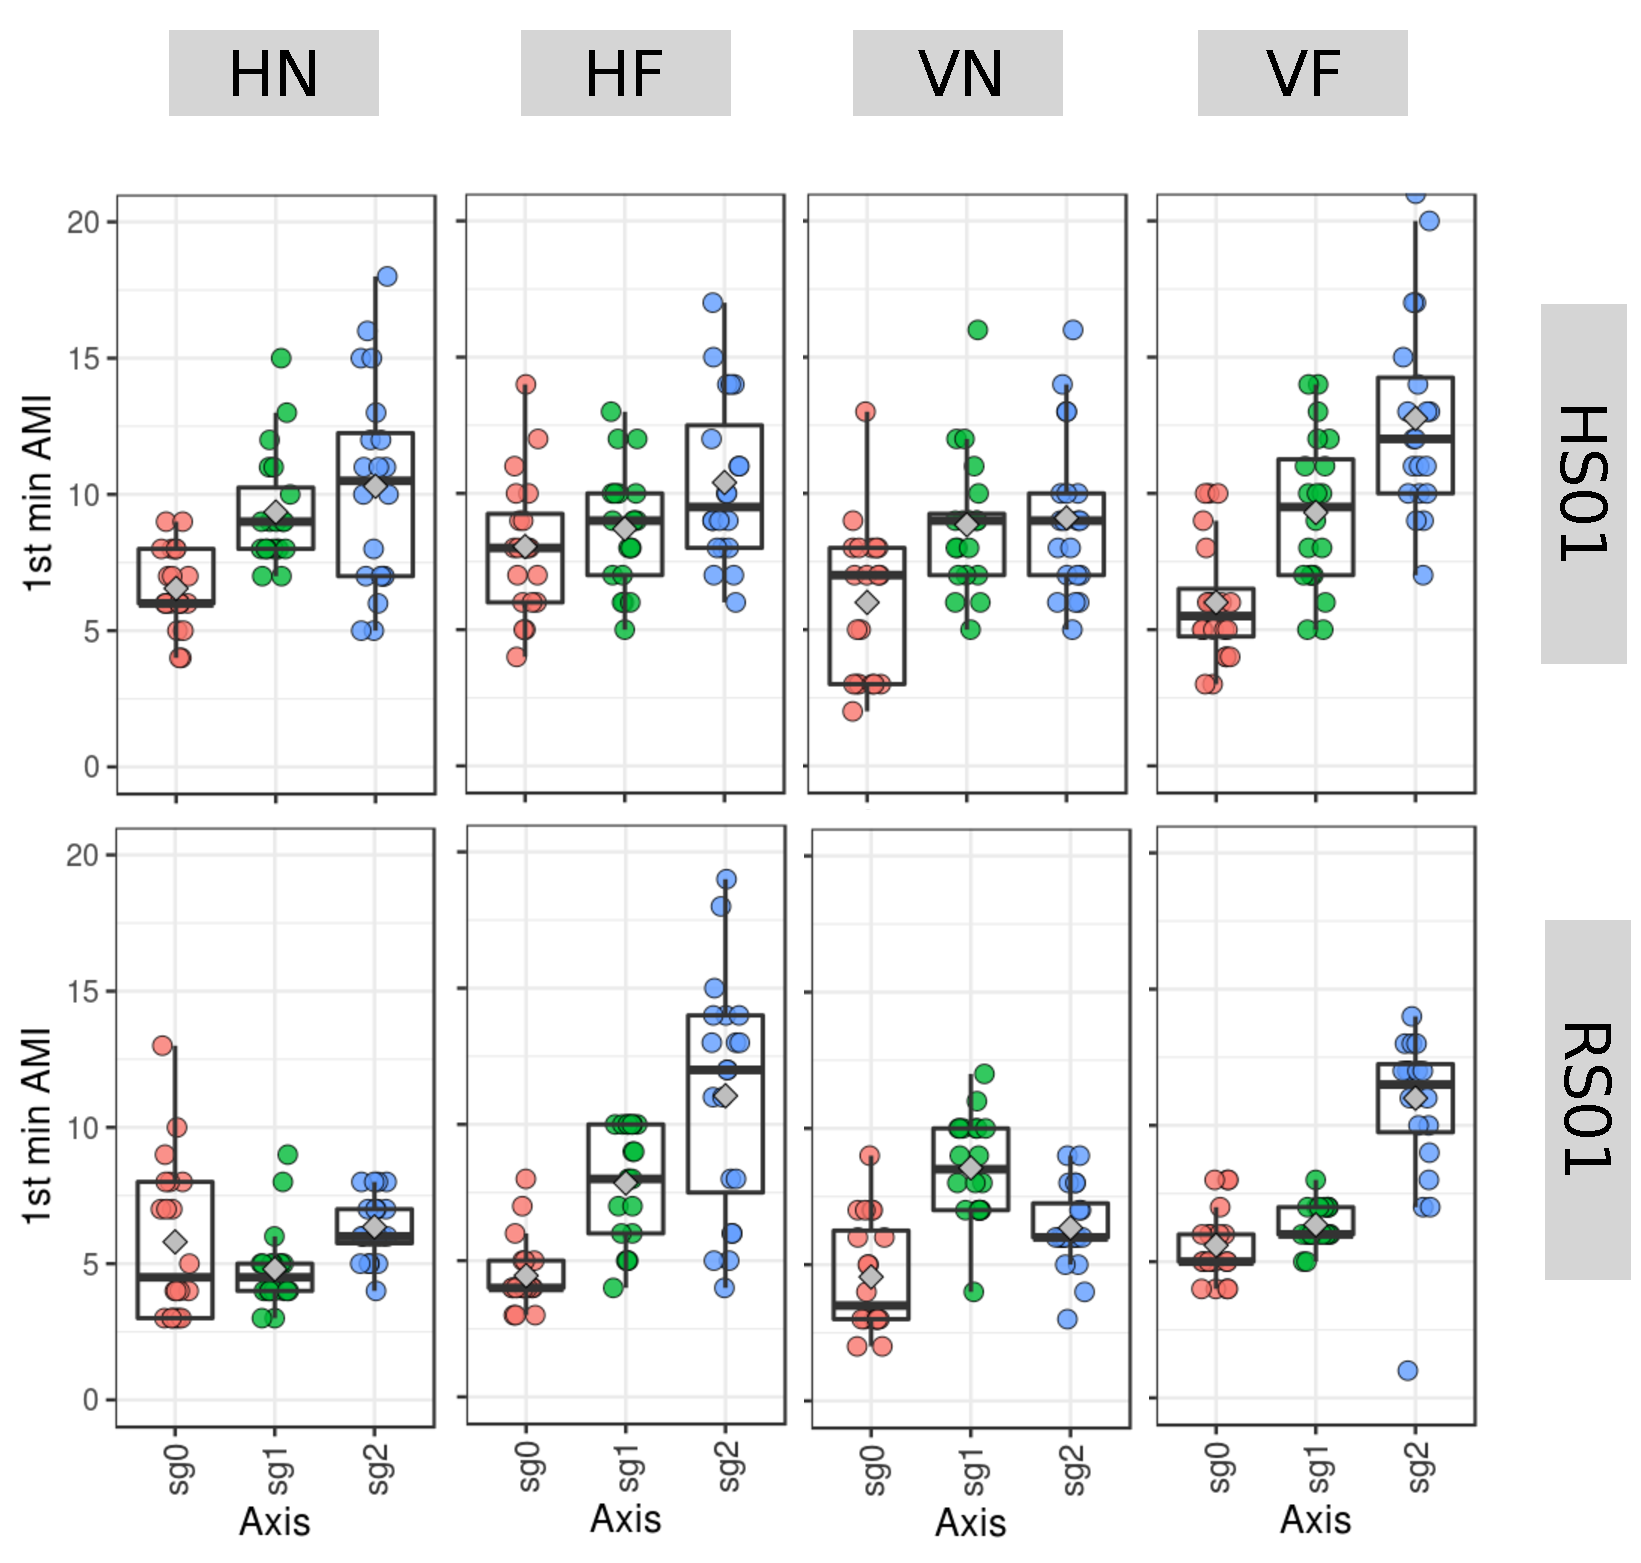
\includegraphics[width=1.0\textwidth]{AMI}
%	\caption{
%	{\bf First minimum AMI values.} 
%		Box plots of first minimum AMI values are for 
%		Horizontal Normal (HN), Horizontal Faster (HF),
%		Vertical Normal (VN) and Vertical Faster (VF)
%		with sensor attached to participants (HS01) and
%		sensor attached to robot (RS01).
%		First inimum AMI values are for twenty participants 
%		($p01$ to $p20$) with three smoothed signals 
%		(sg0zmuvGyroZ (sg0) , sg1zmuvGyroZ (sg1) and sg2zmuvGyroZ (sg2))
%		and window length of 10-sec (500 samples).
%		R code to reproduce the figure is available 
%		from \cite{hwum2018}.
%        }
%    \label{fig:AMI}
%\end{figure}
%%%---------------------------------(FIGURE)------------------------------------
%



\newpage
\subsection{Average minimum embedding parameters}
Following the Section \ref{sec:overall_minMT} to compute the overall average 
of minimum embedding parameters, the sample mean for the 
minimum values of $E_{1}(m)$ from Figs \ref{fig:CAOAMI-hhi}(A) 
is $\overline{m}_0=6$ and the sample 
mean for minimum values of AMIs from Figs~\ref{fig:CAOAMI-hhi}(B)
is $\overline{\tau}_0=8$, for which the overall average minimum embedding 
parameters is ($\overline{m_0}=6$, $\overline{\tau_0}=8$).
Hence, we use the average minimum embedding parameters 
($\overline{m_0}=6$, $\overline{\tau_0}=8$) to compute 
Reconstructed State Spaces (RSSs), Recurrence Plots (RPs) and
Recurrence Quantification Analysis (RQA) metrics for human-humanoid activities.


%\newpage
\section{Reconstructed state spaces with UTDE}
Considering Section \ref{sec:rsswithUTDE} and time series for participant $p01$ 
(Figs \ref{fig:tsH}, \ref{fig:tsV}) the reconstructed state spaces
for horizontal arm movements (Figs~\ref{fig:rss_aHw10}) and
 vertical arm movements  (Figs~\ref{fig:rss_aVw10}) 
are computed with $\overline{m_0}=6$ and $\overline{\tau_0}=8$ 


The trajectories of the RSSs for horizontal normal and faster from 
HS01 and RS01 are slightly smoothed as the time-series 
smoothness increase (Figs~\ref{fig:rss_aHw10}). 
Although the frequency of the movement increase from normal to faster velocity
activities, the trajectories RSSs in Figs~\ref{fig:rss_aHw10}(B)
show highers oscillations specially for a maximum values of smoothness
(sg2zmuvGyroZ), while the trajectories in the RSS for HF in 
Figs~\ref{fig:rss_aHw10}(D) show a lower and smoothed oscillations 
as the smoothness increase.
In contrast, the time series for vertical movements are less noisy and 
well structured (Figs \ref{fig:tsV}) for which the trajectories in the RSSs 
seem to be less organised, specially for Fig \ref{fig:rss_aVw10}(A,C), 
while time series for vertical faster movements (VF) which have more 
periods (Figs \ref{fig:tsV}) present trajectories in the RSS with 
well defined patters (\ref{fig:rss_aVw10}(C,D)).
It is important to note that the smoothness of time series also create 
an effect on smoothness in the trajectories of the RSS, being the RS01 
more organised and more persistent while trajectories for HS01 are 
more changeable (Figs. \ref{fig:rss_aHw10}, \ref{fig:rss_aVw10}).


%%---------------------------------(FIGURE)-------------------------------------
\begin{figure}
\centering
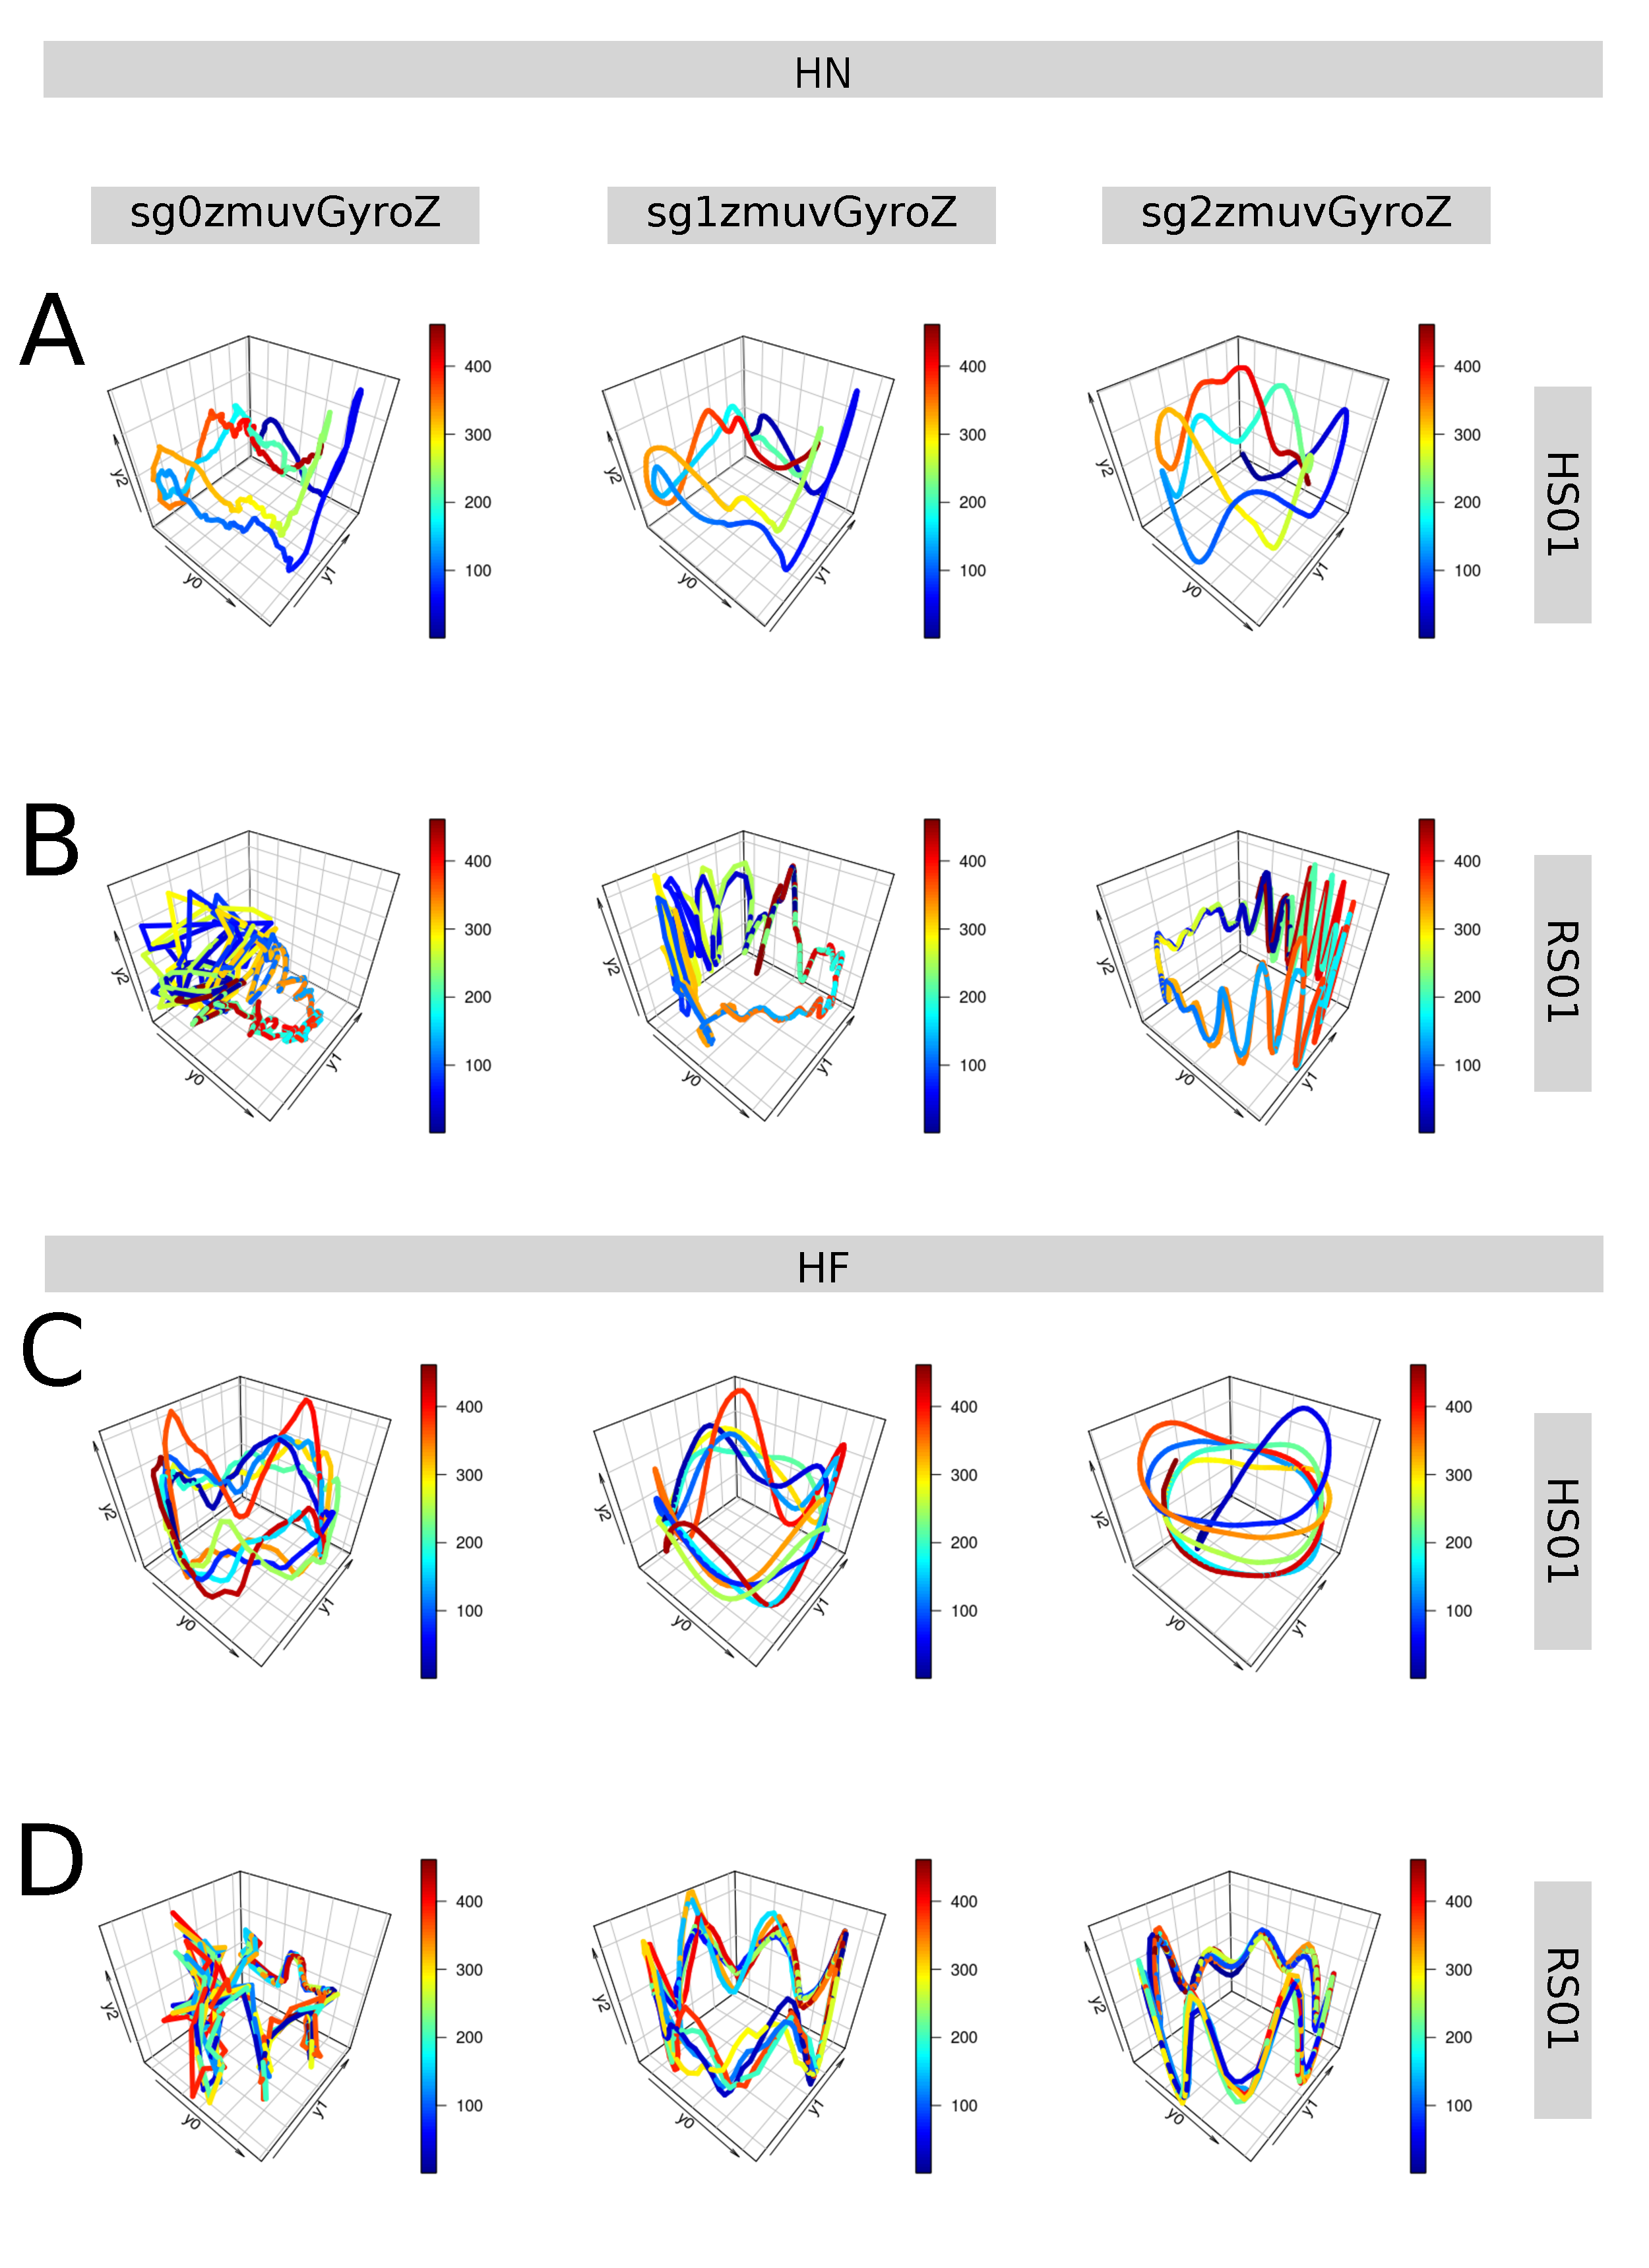
\includegraphics[height=0.85\textheight]{rss_aH}
\caption
	[RSSs for horizontal arm movements]{
	{\bf RSSs for horizontal arm movements.}
	Reconstructed state spaces %for time series of Figure \ref{fig:tsH}.
	of participant p01 for horizontal movements in normal and faster 
	velocity (HN, HF) with raw-normalised (sg0zmuvGyroZ), 
	normalised-smoothed 1 (sg1zmuvGyroZ) and 
	normalised-smoothed 2 (sg2zmuvGyroZ) time series of the 
	sensors attached to the participant (HS01) and other sensor 
	attached to the robot (RS01).	
	Reconstructed state spaces were computed with 
	embedding parameters $m=6$, $\tau=8$.
	R code to reproduce the figure is available from \cite{hwum2018}.
        }
    \label{fig:rss_aHw10}
\end{figure}
%%---------------------------------(FIGURE)------------------------------------



%%---------------------------------(FIGURE)-------------------------------------
\begin{figure}
\centering
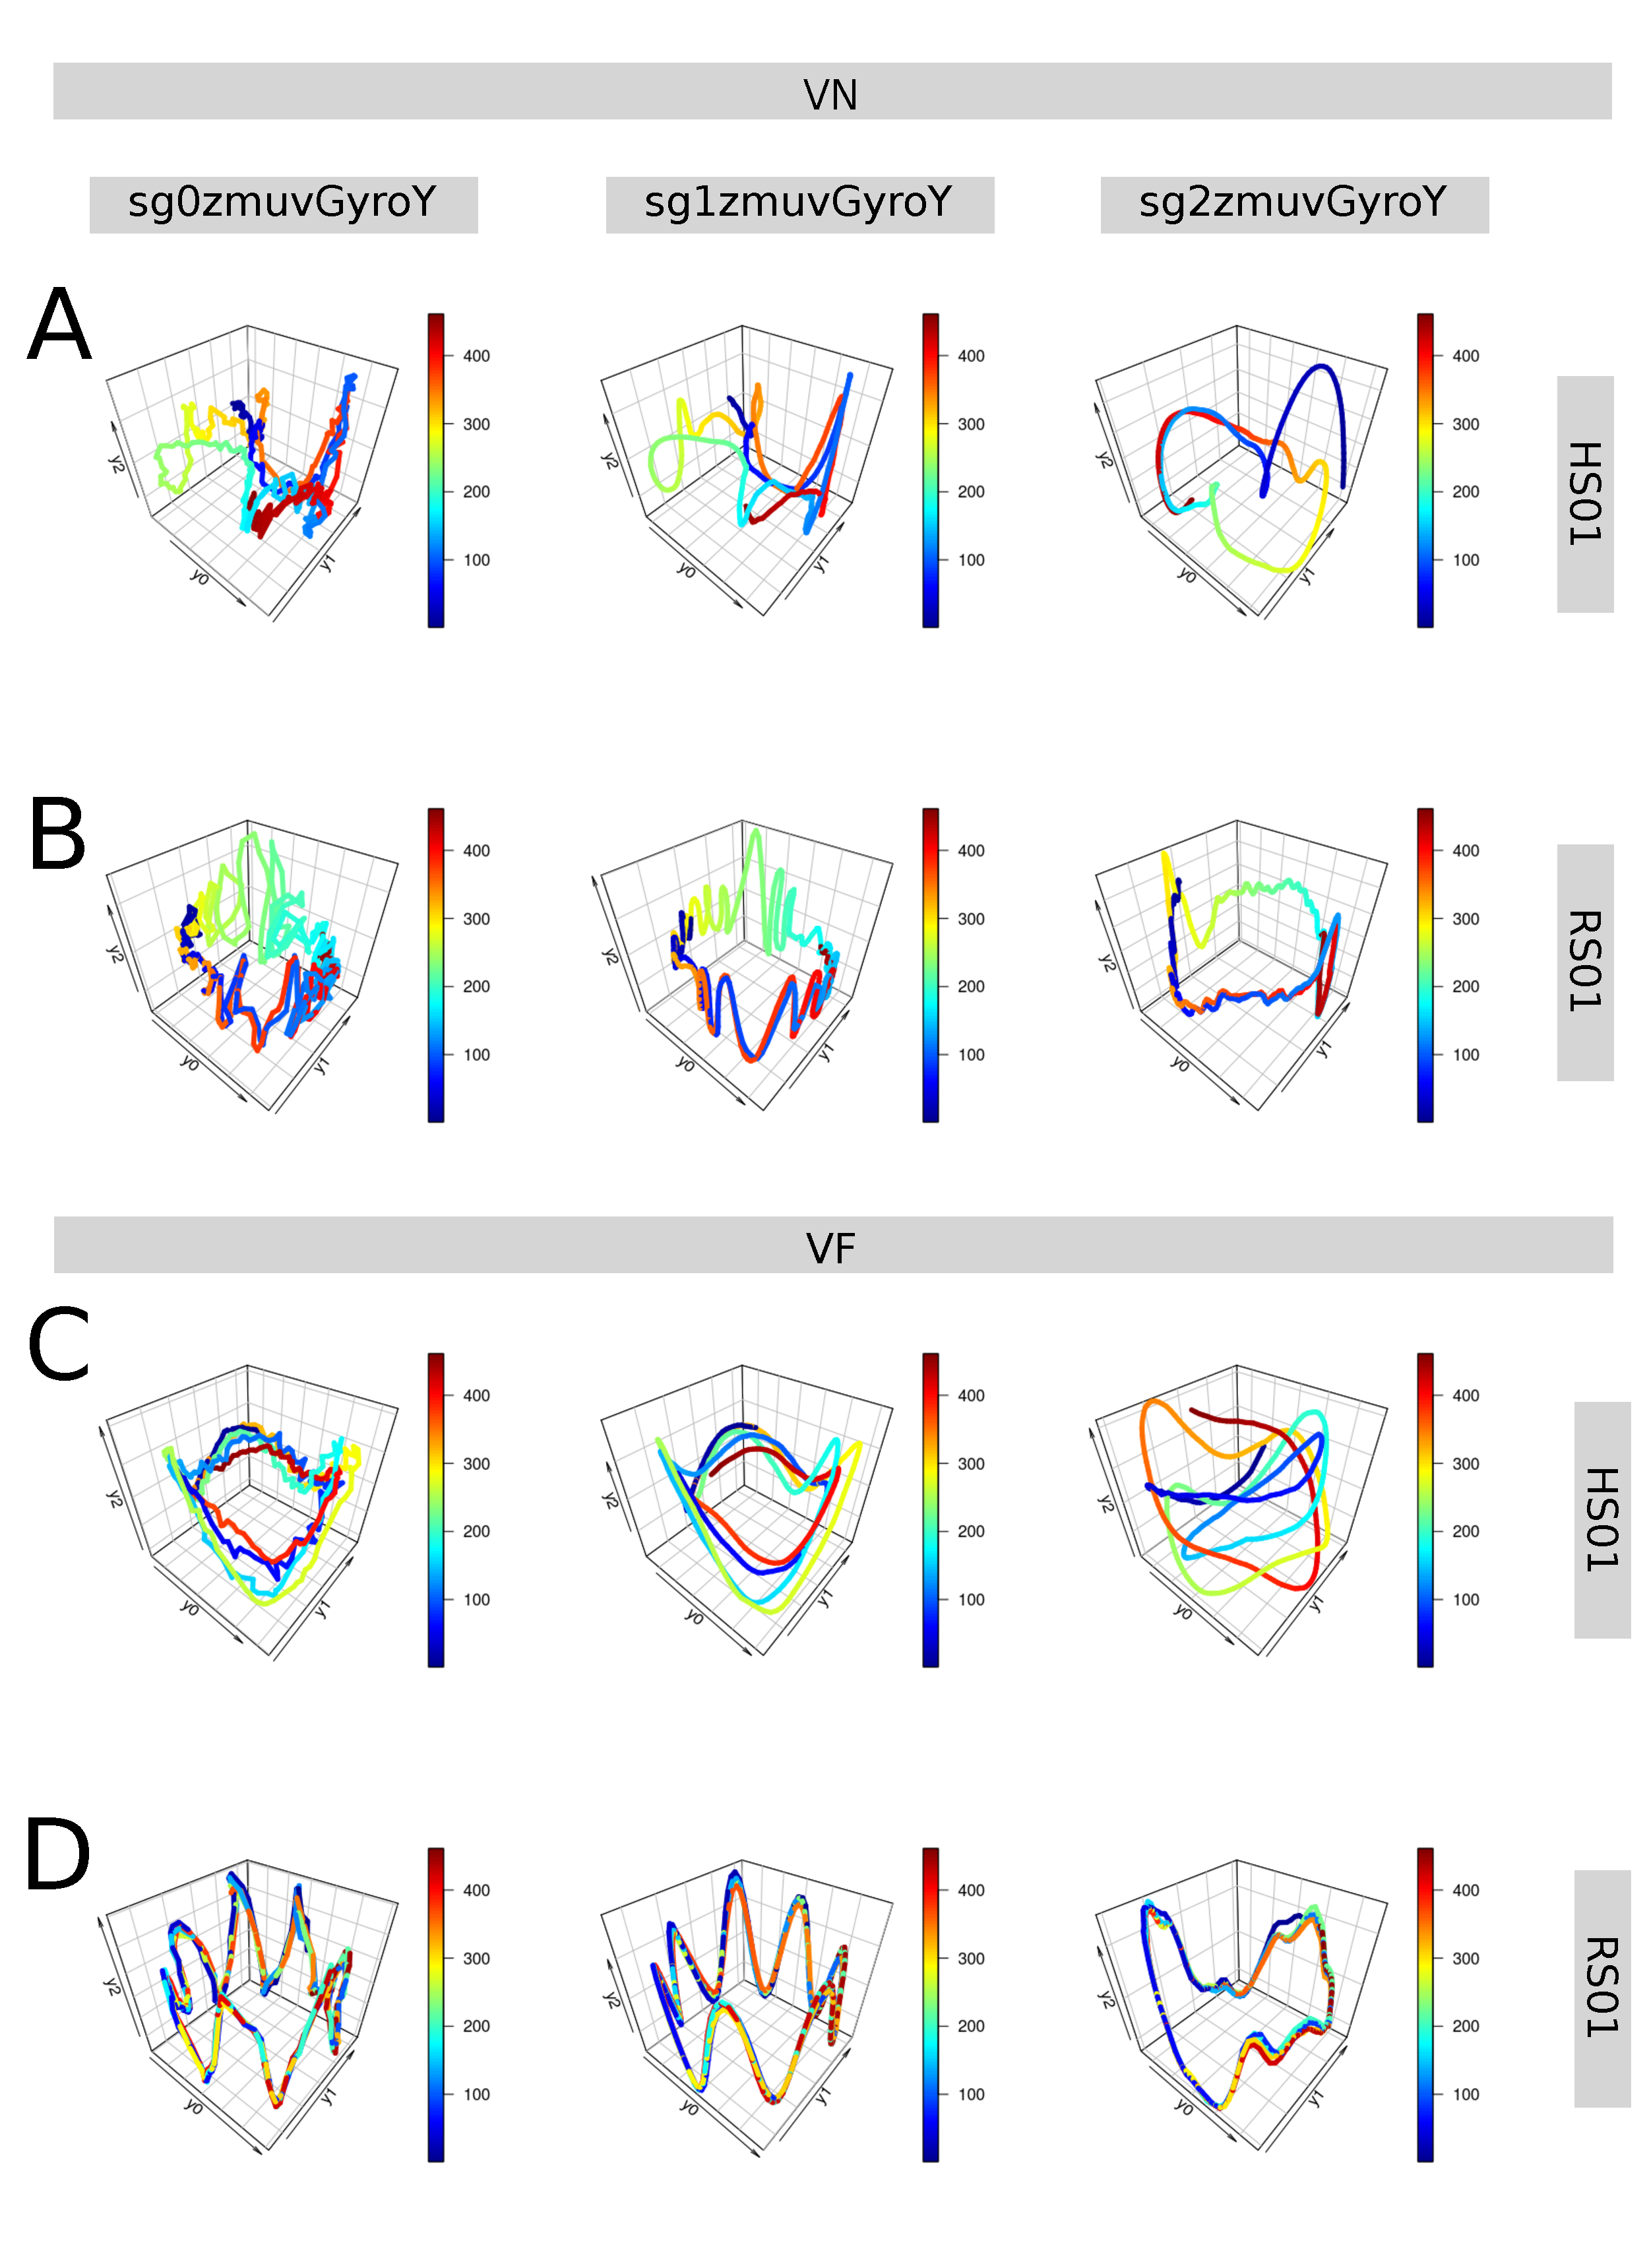
\includegraphics[height=0.85\textheight]{rss_aV}
    \caption
	[RSSs for vertical arm movements]{
	{\bf RSSs for vertical arm movements.}
	Reconstructed state spaces %for time series of Figure \ref{fig:tsV}.
	of participant p01 for vertical movements in normal and faster 
	velocity (VN, VF) with raw-normalised (sg0zmuvGyroZ), 
	normalised-smoothed 1 (sg1zmuvGyroZ) and 
	normalised-smoothed 2 (sg2zmuvGyroZ) time series of the 
	sensors attached to the participant (HS01) and other sensor 
	attached to the robot (RS01).	
	Reconstructed state spaces were computed with 
	embedding parameters $m=6$, $\tau=8$.
	R code to reproduce the figure is available from \cite{hwum2018}.
        }
    \label{fig:rss_aVw10}
\end{figure}
%%---------------------------------(FIGURE)------------------------------------

Therefore, one can observe by eye the differences in each of the trajectories 
in the reconstructed state spaces 
(Figs~\ref{fig:rss_aHw10}, \ref{fig:rss_aVw10}), 
however one might be not objective when quantifying those differences 
since such observations might vary from person to person.
With that in mind, in our early experiments, we tried to objectively 
quantify those differences using euclidean distances between 
the origin to each of the points in the trajectories in the trajectories of 
the RSSs, however these created suspicious metrics, specially 
for trajectories which looked very messy.
Hence, we proposed to apply Recurrence Quantification Analyses (RQA) 
in order to have a more objective quantification of the differences 
in each of the cases of the time series.


\newpage
\section{Recurrences Plots}
Considering the time series of Figs~\ref{fig:tsH} and \ref{fig:tsV}, 
we computed its Recurrence Plots for horizontal arm movements 
(Fig~\ref{fig:rp_aH}) and vertical arm movements (Fig~\ref{fig:rp_aV}) 
using the average embedding parameters ($m=6$, $\tau=8$) and a recurrence 
threshold of $\epsilon=1$. For the selection of the recurrence threshold,
\cite{marwan2011} pointed out that choosing an appropriate 
recurrence threshold is crucial to get meaningful representations in the RPs, 
however, for this thesis where quantifying movement variability is our aim,
we give little importance to the selection of the recurrence threshold 
for the RPs as long as it is able to represent the dynamical transitions 
in each of the time series.

In general, the increase of smoothness in time series results in thicker 
and better defined diagonal lines in the RPs 
(Figs~\ref{fig:rp_aH}, \ref{fig:rp_aV}).
Additionally, due to the changes in velocities of the movements 
the patterns in the RPs present an increase of diagonal lines 
and a decrease of line thickness.
%(Figs~\ref{fig:rp_aH}, \ref{fig:rp_aV}).
Although, the patterns of RPs show consistency with the movements type 
and velocities changes, it can be noticed that patterns of the RPs for 
HS01 are not well defined while patterns of the RPs for RS01 
shown a more consistent pattern (Fig~\ref{fig:rp_aH}, \ref{fig:rp_aV}). 

It is important to note that only RPs for participant 01 are presented
in (Fig~\ref{fig:rp_aV}, \ref{fig:rp_aH}), however
other RPs for all participants are presented in Appendix \ref{appendix:d:rps}.
With that in mind, we can highlight that, as similar as, the 
Reconstructed State Spaces (Figs~\ref{fig:rss_aHw10}, \ref{fig:rss_aVw10}), 
the patterns in the RPs can be easily noticed by eye for different conditions 
of the time series (Figs~\ref{fig:rp_aH}, Fig~\ref{fig:rp_aV}),
however these characteristics in the patterns of the RPs are subjective 
for the person who analysed them and might vary from person to person. 
That lead us to apply Recurrence Quantification Analysis (RQA) in order 
to have an objective quantification metric for the movement variability 
for each of the conditions of the time series.
%%---------------------------------(FIGURE)-------------------------------------
\begin{figure}
\centering
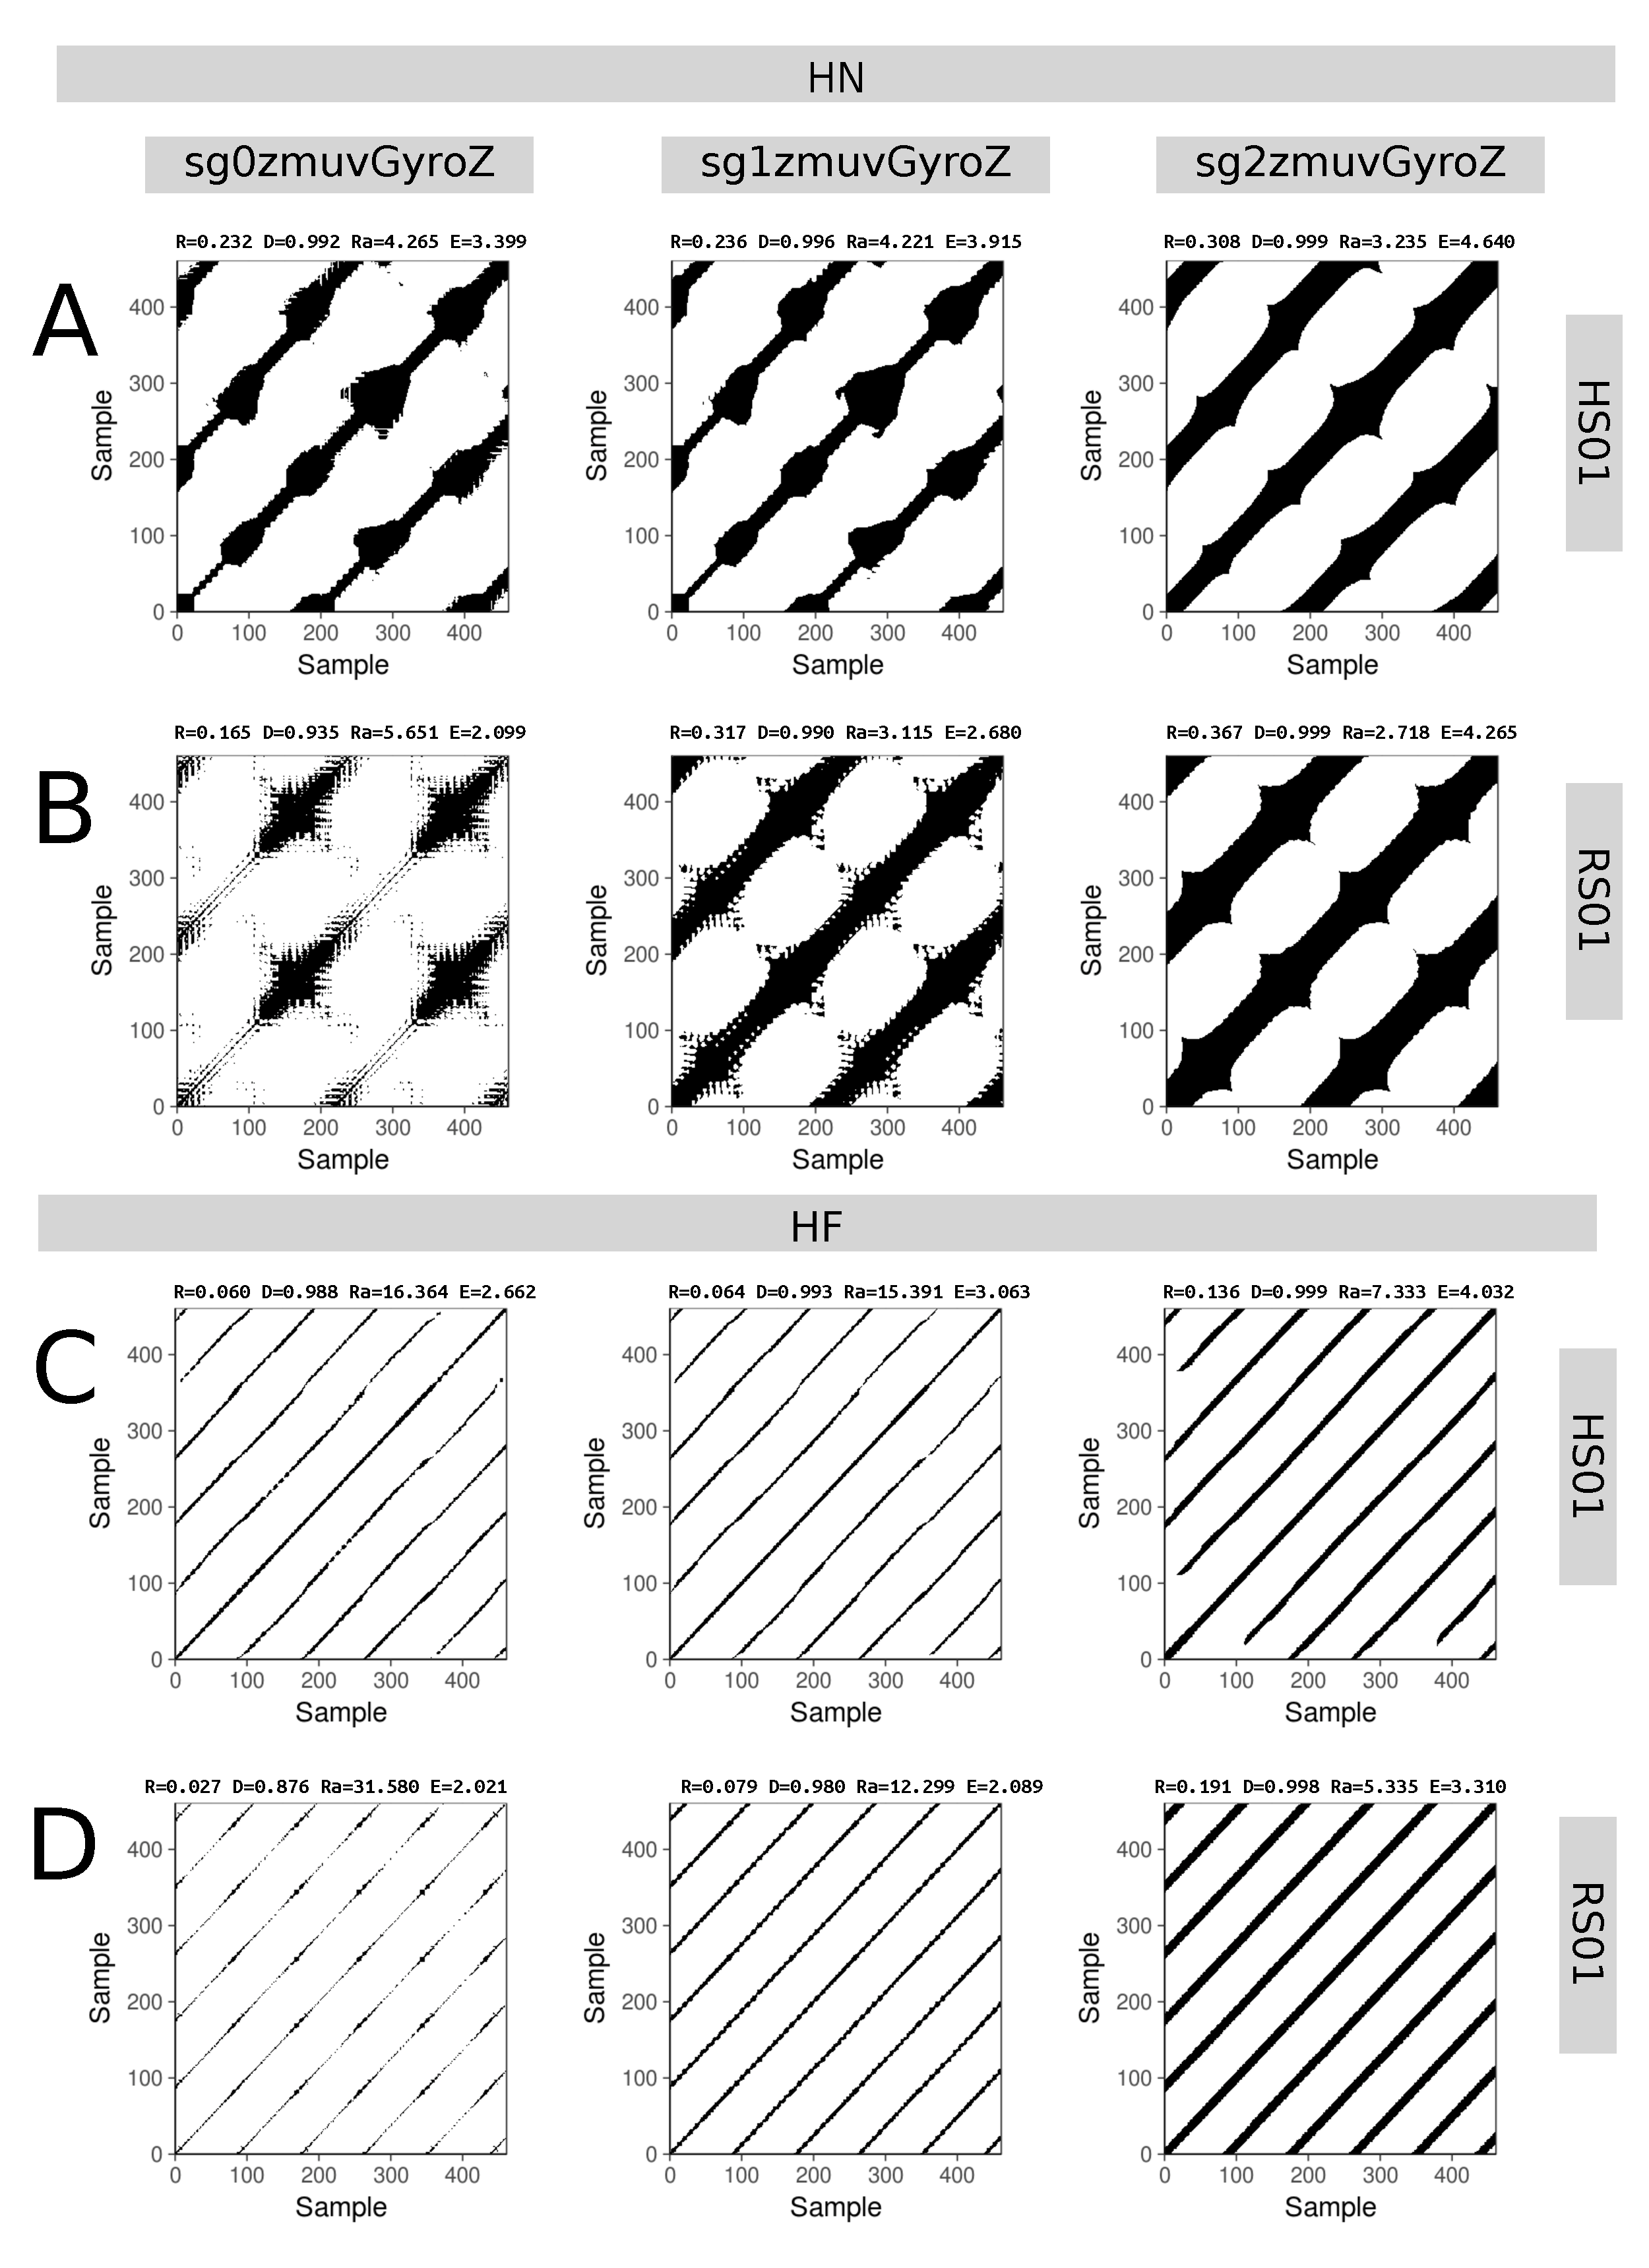
\includegraphics[height=0.80\textheight]{rp_aH}
\caption
	[RPs for horizontal arm movements]{
	{\bf RPs for horizontal arm movements.}	
	Recurrence plots %for time series of Figure \ref{fig:tsV}.
	of participant $p01$ for horizontal movements in normal and faster 
	velocity (HN, HF) with time series of raw-normalised (sg0zmuvGyroZ), 
	normalised-smoothed 1 (sg1zmuvGyroZ) and 
	normalised-smoothed 2 (sg2zmuvGyroZ), and 
	sensors attached to the participant (HS01) and to the robot (RS01).
	Recurrence plots were computed with 
	embedding parameters $m=6$, $\tau=8$ and $\epsilon=1$.
	R code to reproduce the figure is available from \cite{hwum2018}.
        }
    \label{fig:rp_aH}
\end{figure}
%%---------------------------------(FIGURE)------------------------------------
%%---------------------------------(FIGURE)-------------------------------------
\begin{figure}
\centering
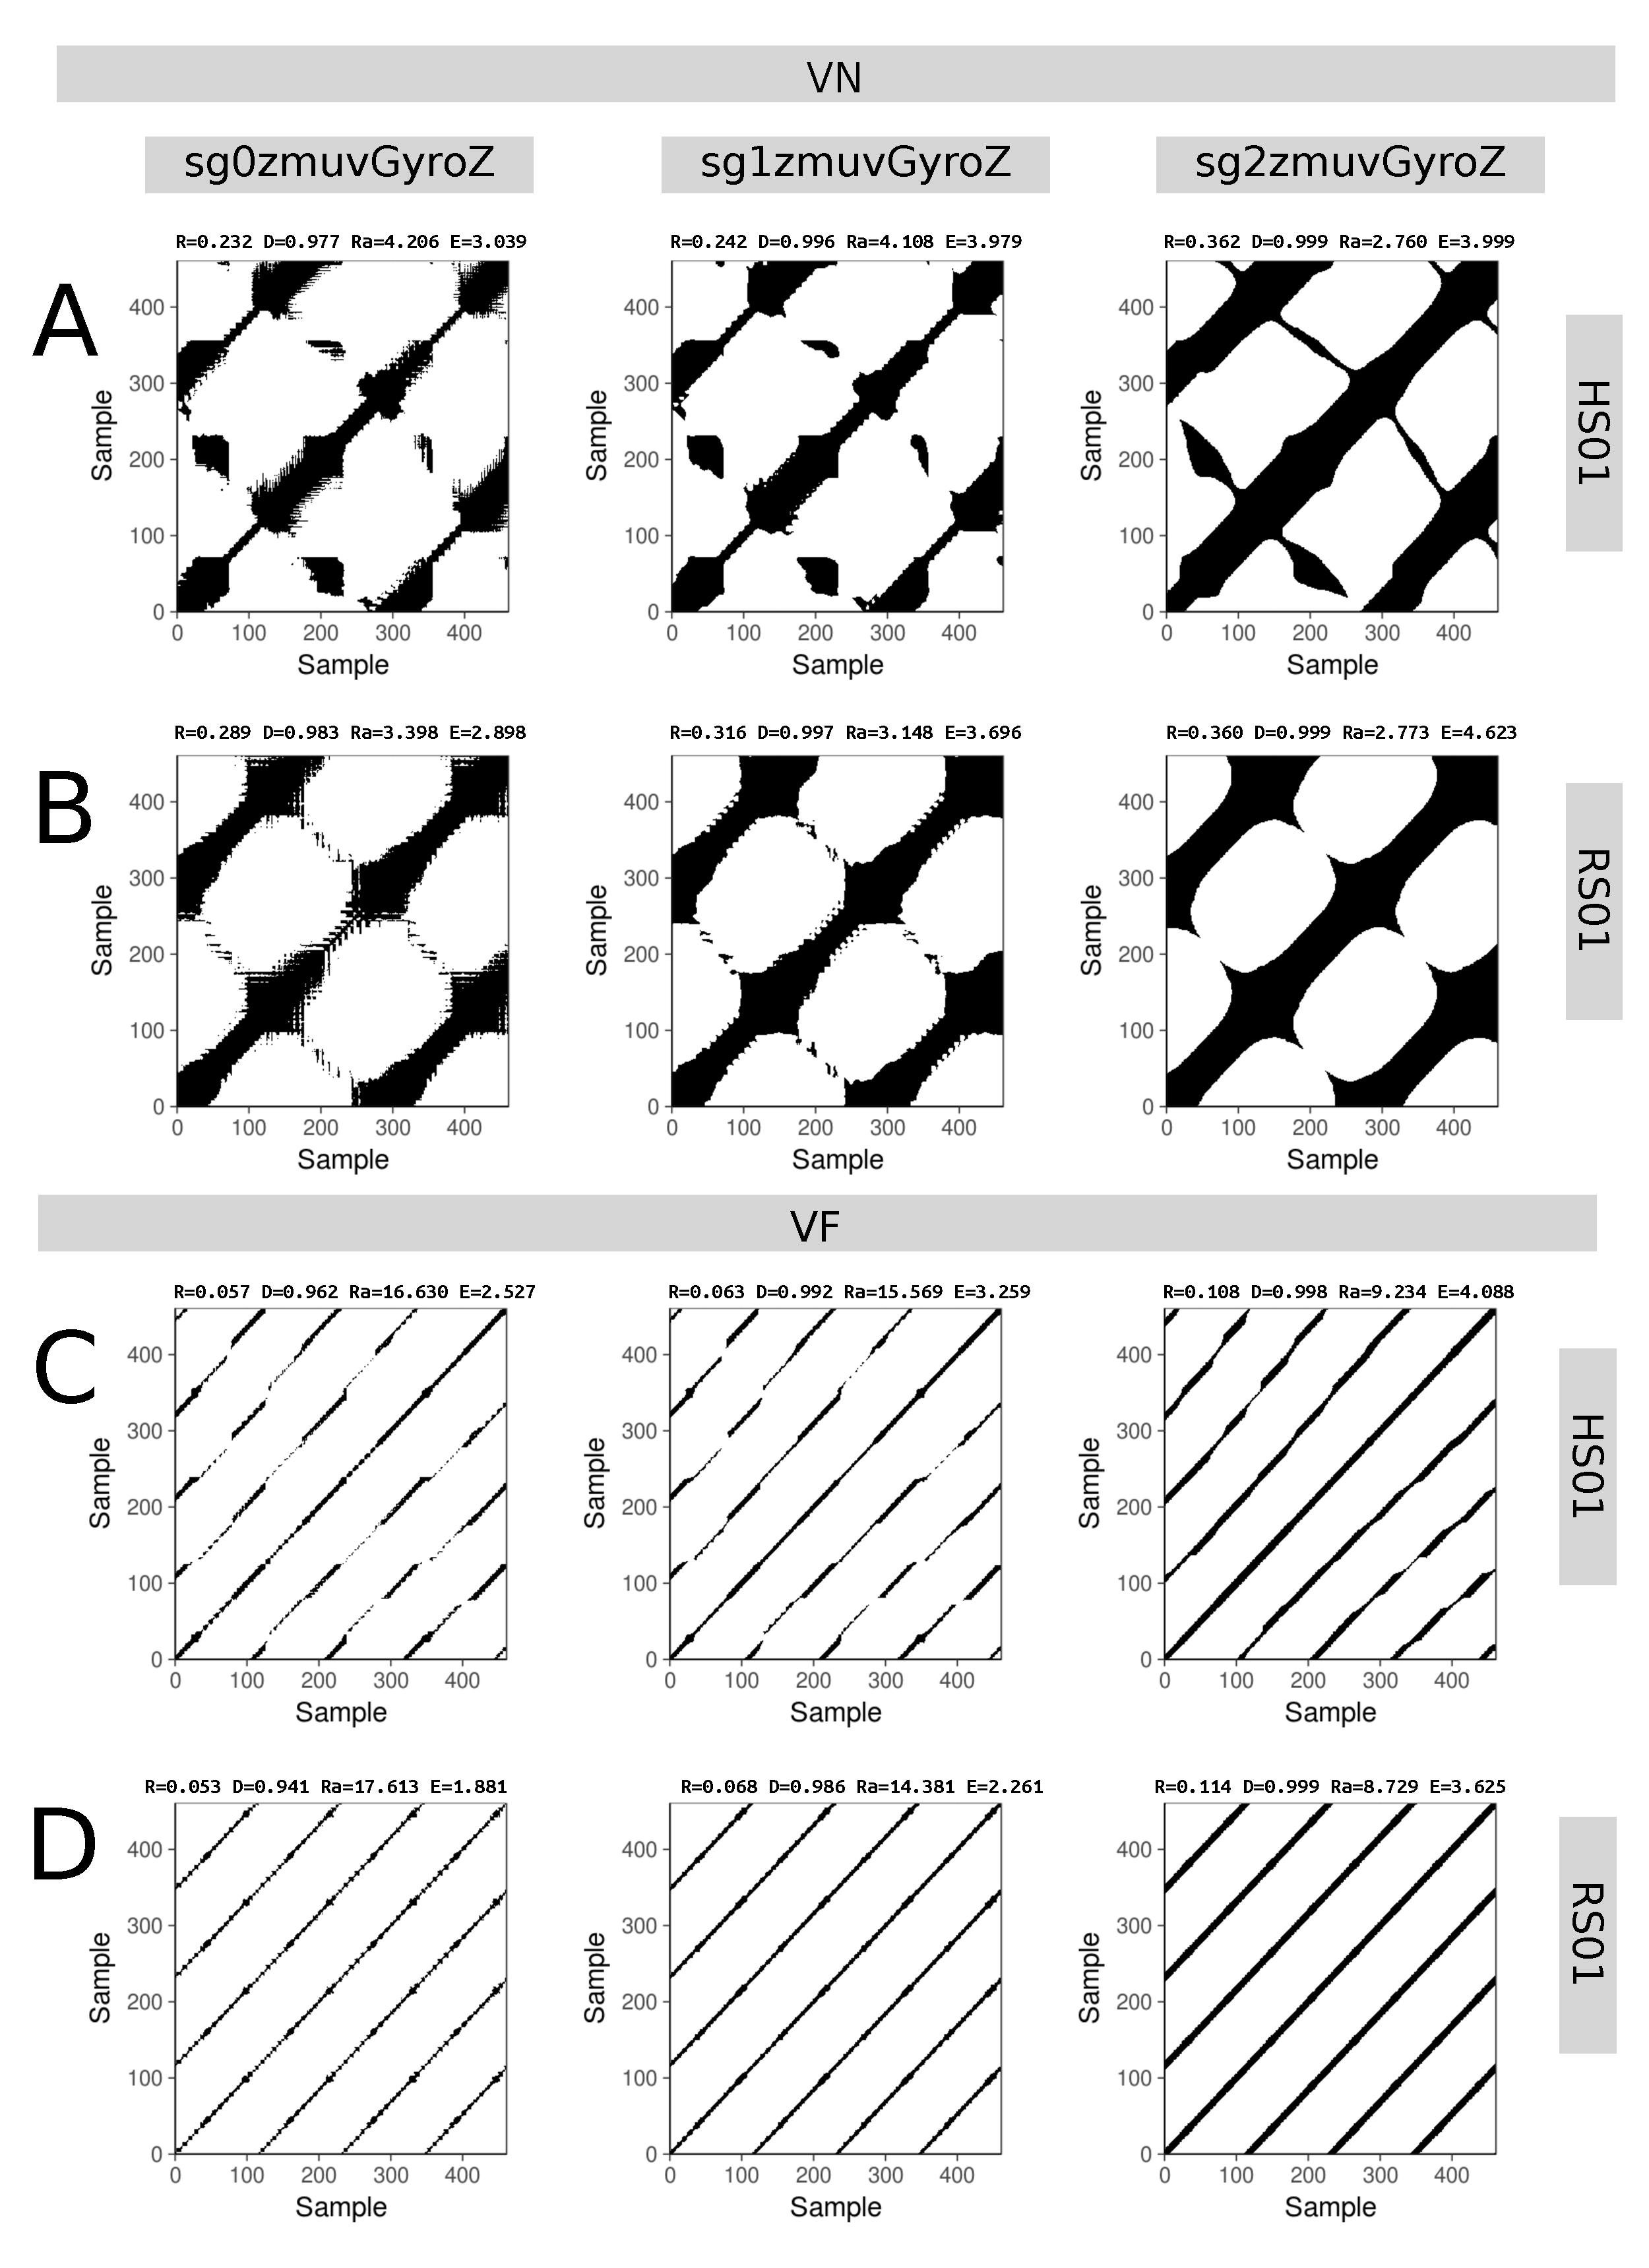
\includegraphics[height=0.80\textheight]{rp_aV}
\caption
	[RPs for vertical arm movements]{
	{\bf RPs for vertical arm movements.}	
	Recurrence plots %for time series of Figure \ref{fig:tsV}.
	of participant $p01$ for vertical movements in normal and faster 
	velocity (VN, VF) with time series of raw-normalised (sg0zmuvGyroZ), 
	normalised-smoothed 1 (sg1zmuvGyroZ) and 
	normalised-smoothed 2 (sg2zmuvGyroZ), and 
	sensors attached to the participant (HS01) and to the robot (RS01).
	Recurrence plots were computed with 
	embedding parameters $m=6$, $\tau=8$ and $\epsilon=1$.
	R code to reproduce the figure is available from \cite{hwum2018}.
        }
    \label{fig:rp_aV}
\end{figure}
%%---------------------------------(FIGURE)------------------------------------




\newpage
\section{Recurrence Quantification Analysis} \label{ch6:rqas}
Considering the RPs for 20 participants performing four activities 
(HN, HF, VN and VF) with sensors attached to the human (HS01) and to the 
humanoid robot (RS01) and with the increase of smoothness of time series 
(sg0zmuvGyroZ, sg1zmuvGyroZ and sg2zmuvGyroZ), 
we hence compute four metrics of RQA metrics (REC, DET, RATIO and ENTR) with 
embedding parameters $m=6$, $\tau=8$ and recurrence threshold $\epsilon=1$.
 

%\newpage
\subsection*{REC values}
It can be seen in the box plots of Figs~\ref{fig:RQABP}(A) that REC values, 
representing the \% of black dots in the RPs, 
are more spread for HN and VN movements (higher interquartile range) 
than HF and VF movements (lower interquartile range) for HS01 sensor. 
In contrast, REC values for RS01 sensor present little variation 
(interquartile range of 0.01).
With regard to the increase of smoothness of time series 
(sg0, sg1 and sg2), REC values present little 
variation as the smoothness is increasing for time series from HS01 
(changes of mean values (rhombus)) while REC values are more affected with 
the smoothness for data from RS01 
(see the incremental changes of mean values (rhombus)).
See Figs~\ref{fig:rec_aH} and \ref{fig:rec_aV} in appendix \ref{appendix:e:ep} 
for more details about individual REC values for each participant.
%%%---------------------------------(FIGURE)-------------------------------------
%\begin{figure}
%\centering
%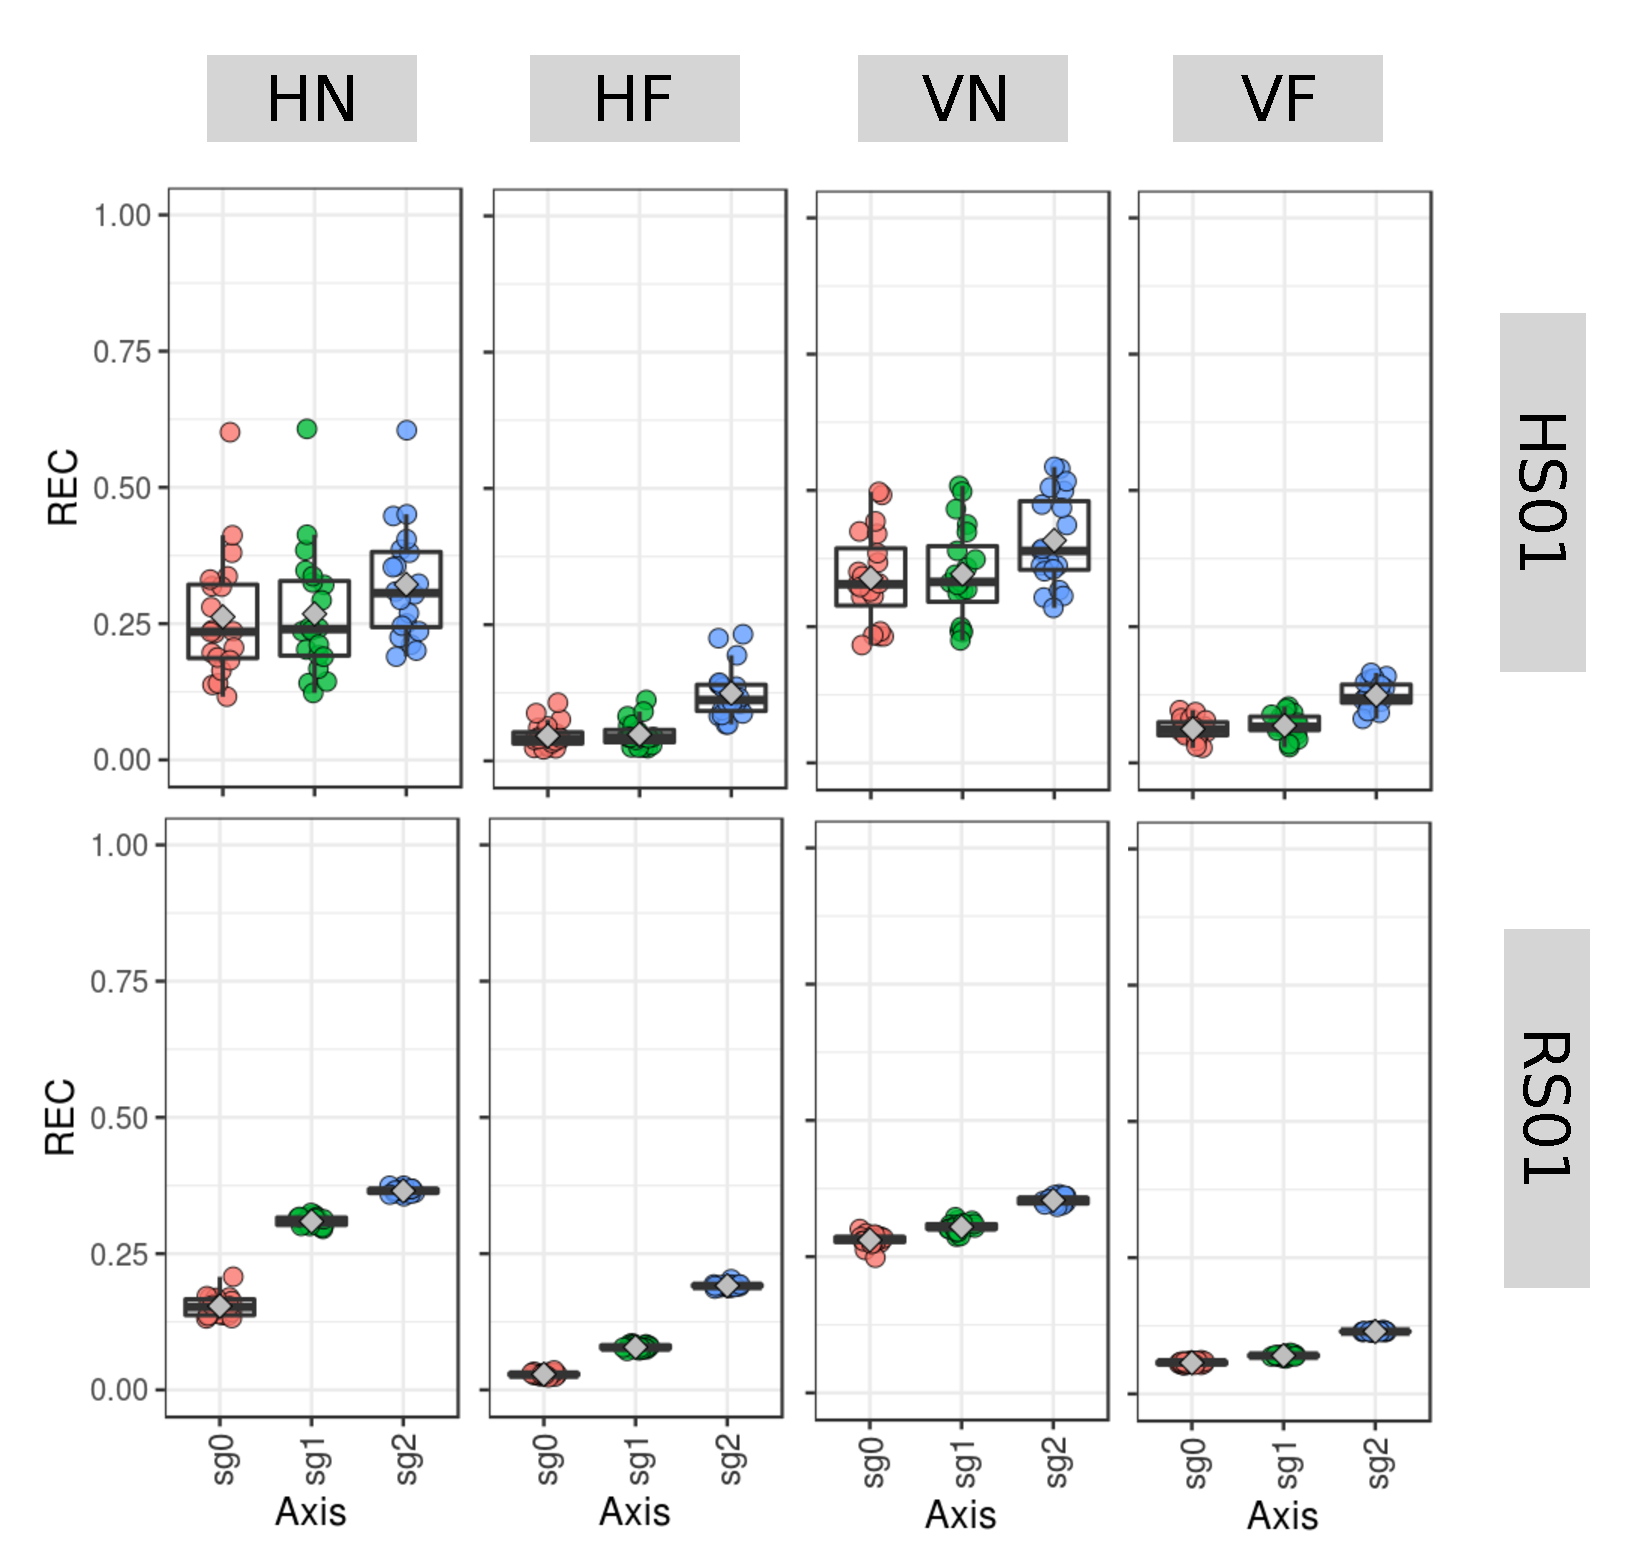
\includegraphics[width=0.6\textwidth]{rec-bp}
%    \caption{
%	{\bf Box plots for REC values.}	
%	REC values (representing \% of black dots in the RPs) for 
%	20 participants performing HN, HF, VN and VF movements
%	with sensors HS01, RS01 and three smoothed-normalised 
%	time series (sg0, sg1 and sg2).
%	REC values were computed with 
%	embedding parameters $m=6$, $\tau=8$ and $\epsilon=1$.
%	R code to reproduce the figure is available from \cite{hwum2018}.
%        }
%    \label{fig:REC}
%\end{figure}
%%%---------------------------------(FIGURE)------------------------------------
%


%\newpage
\subsection*{DET values}
Figs \ref{fig:RQABP}(B) illustrate DET values, 
representing predictability and organisation of the RPs, 
which change very little (interquartile range is around 0.1) 
for type of movement, level of smoothness or type of sensor.
See Figs~\ref{fig:det_aH} and \ref{fig:det_aV} in appendix \ref{appendix:e:ep} 
for more details about individual DET values for each participant.
%

%%%---------------------------------(FIGURE)-------------------------------------
%\begin{figure}
%\centering
%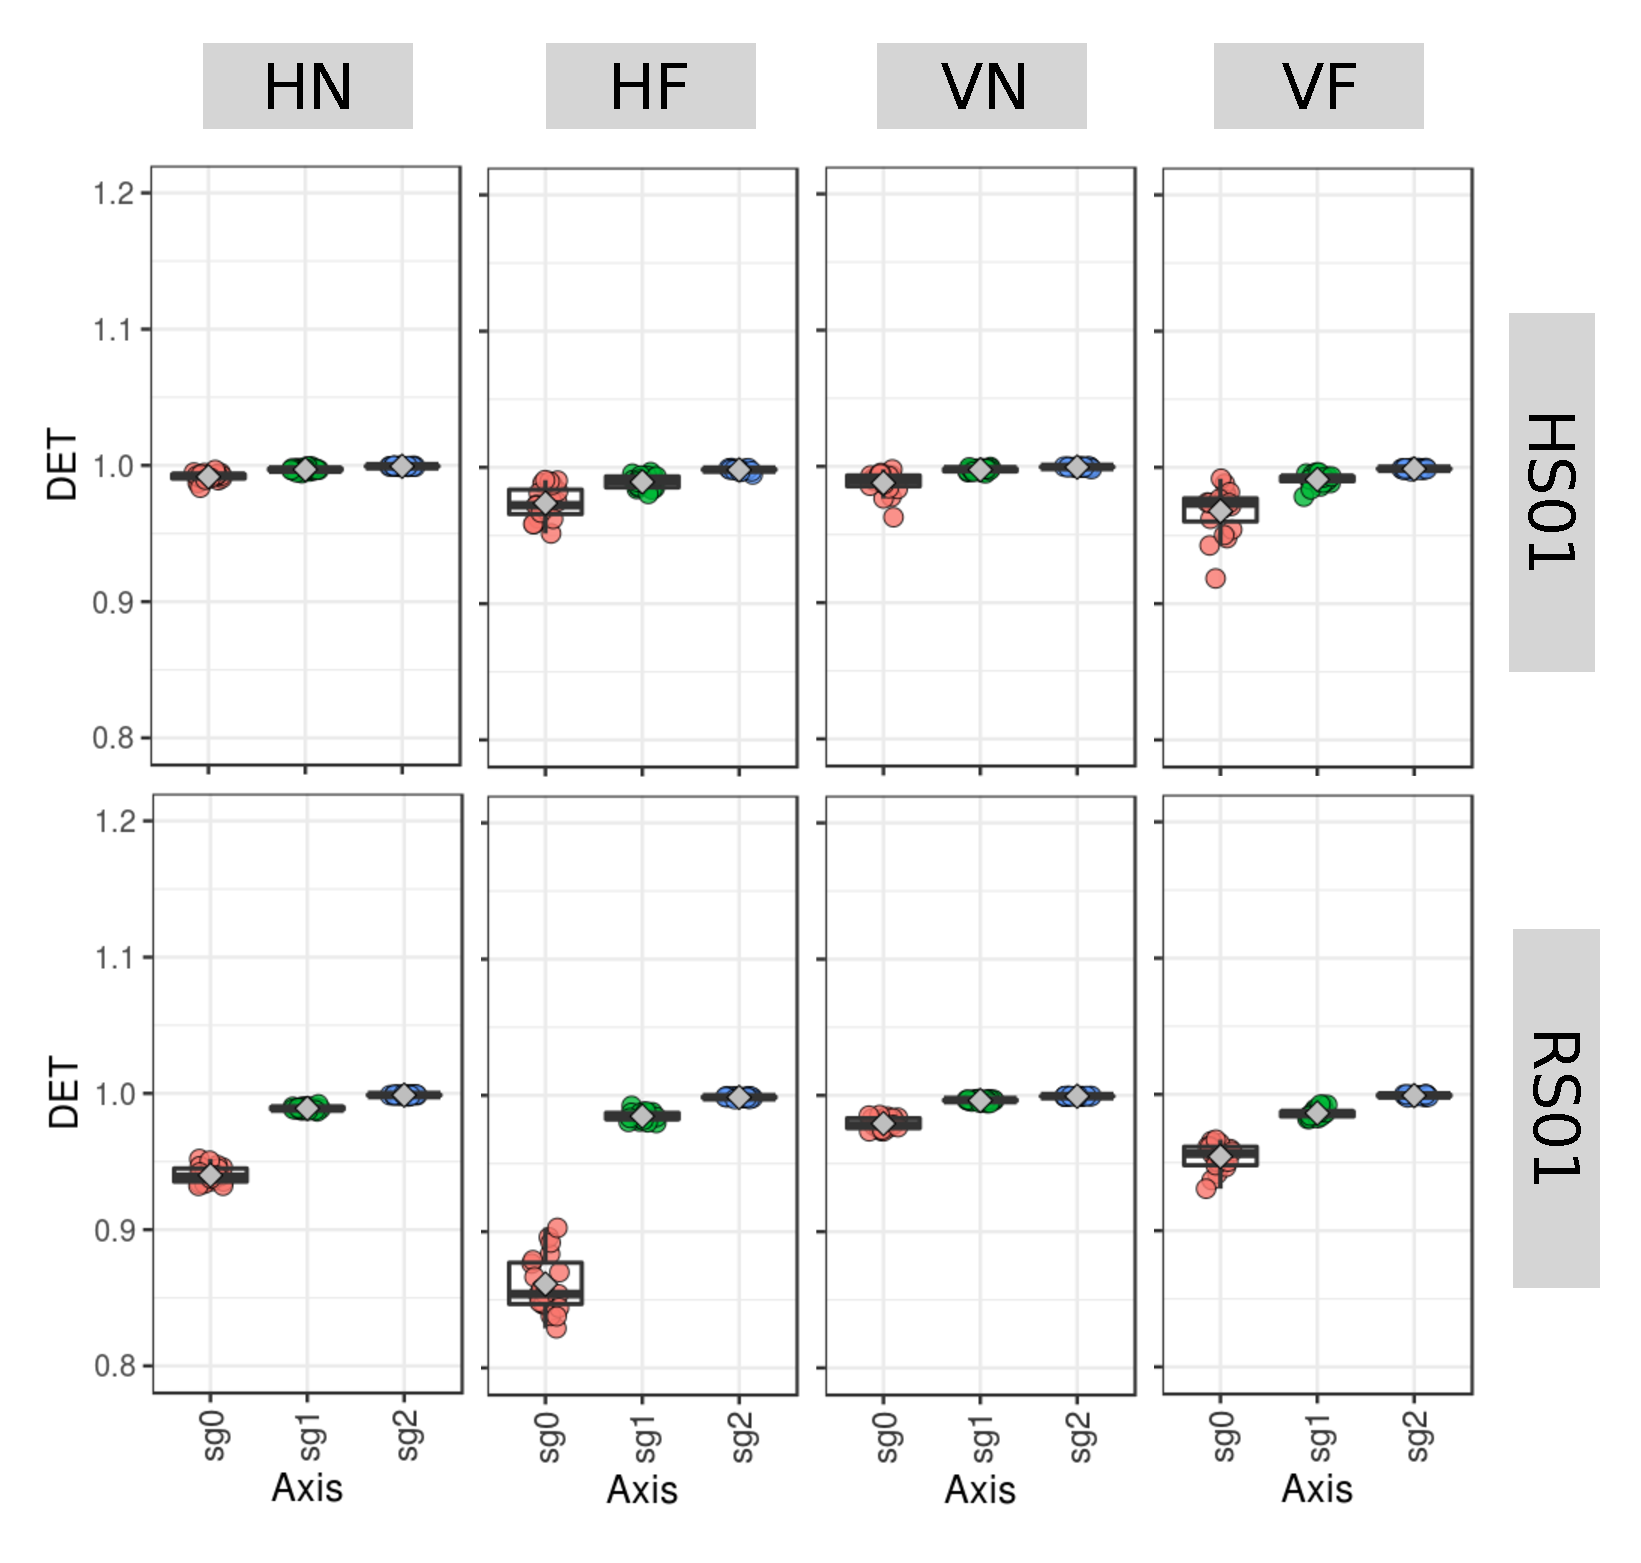
\includegraphics[width=0.6\textwidth]{det-bp}
%    \caption{
%	{\bf Box plots for DET values.}	
%    	DET values (representing predictability and organisation of the RPs)
%	for 20 participants performing HN, HF, VN and VF movements
%	with sensors HS01, RS01 and three smoothed-normalised 
%	time series (sg0, sg1 and sg2).
%	DET values were computed with 
%	embedding parameters $m=6$, $\tau=8$ and $\epsilon=1$.
%	R code to reproduce the figure is available from \cite{hwum2018}.
%        }
%    \label{fig:DET}
%\end{figure}
%%%---------------------------------(FIGURE)------------------------------------
%

%\newpage
\subsection*{RATIO values}
Figs \ref{fig:RQABP}(C) present RATIO values, representing dynamic transitions, 
for horizontal and vertical movements.
It can be seen that RATIO values for HS01 sensor vary less 
for HN movements (interquartile range around 2)
than HF movements (interquartile range around 5).
%which is a similar behaviour of RATIO values for oRS01 sensor.
It can also be noticed a decrease of variation in RATIO values as the 
smoothness of the time series is increasing (grey rhombus).
See Figs~\ref{fig:ratio_aH} and \ref{fig:ratio_aV} in appendix 
\ref{appendix:e:ep} 
for more details about individual RATIO values for each participant.
%%%---------------------------------(FIGURE)-------------------------------------
%\begin{figure}
%\centering
%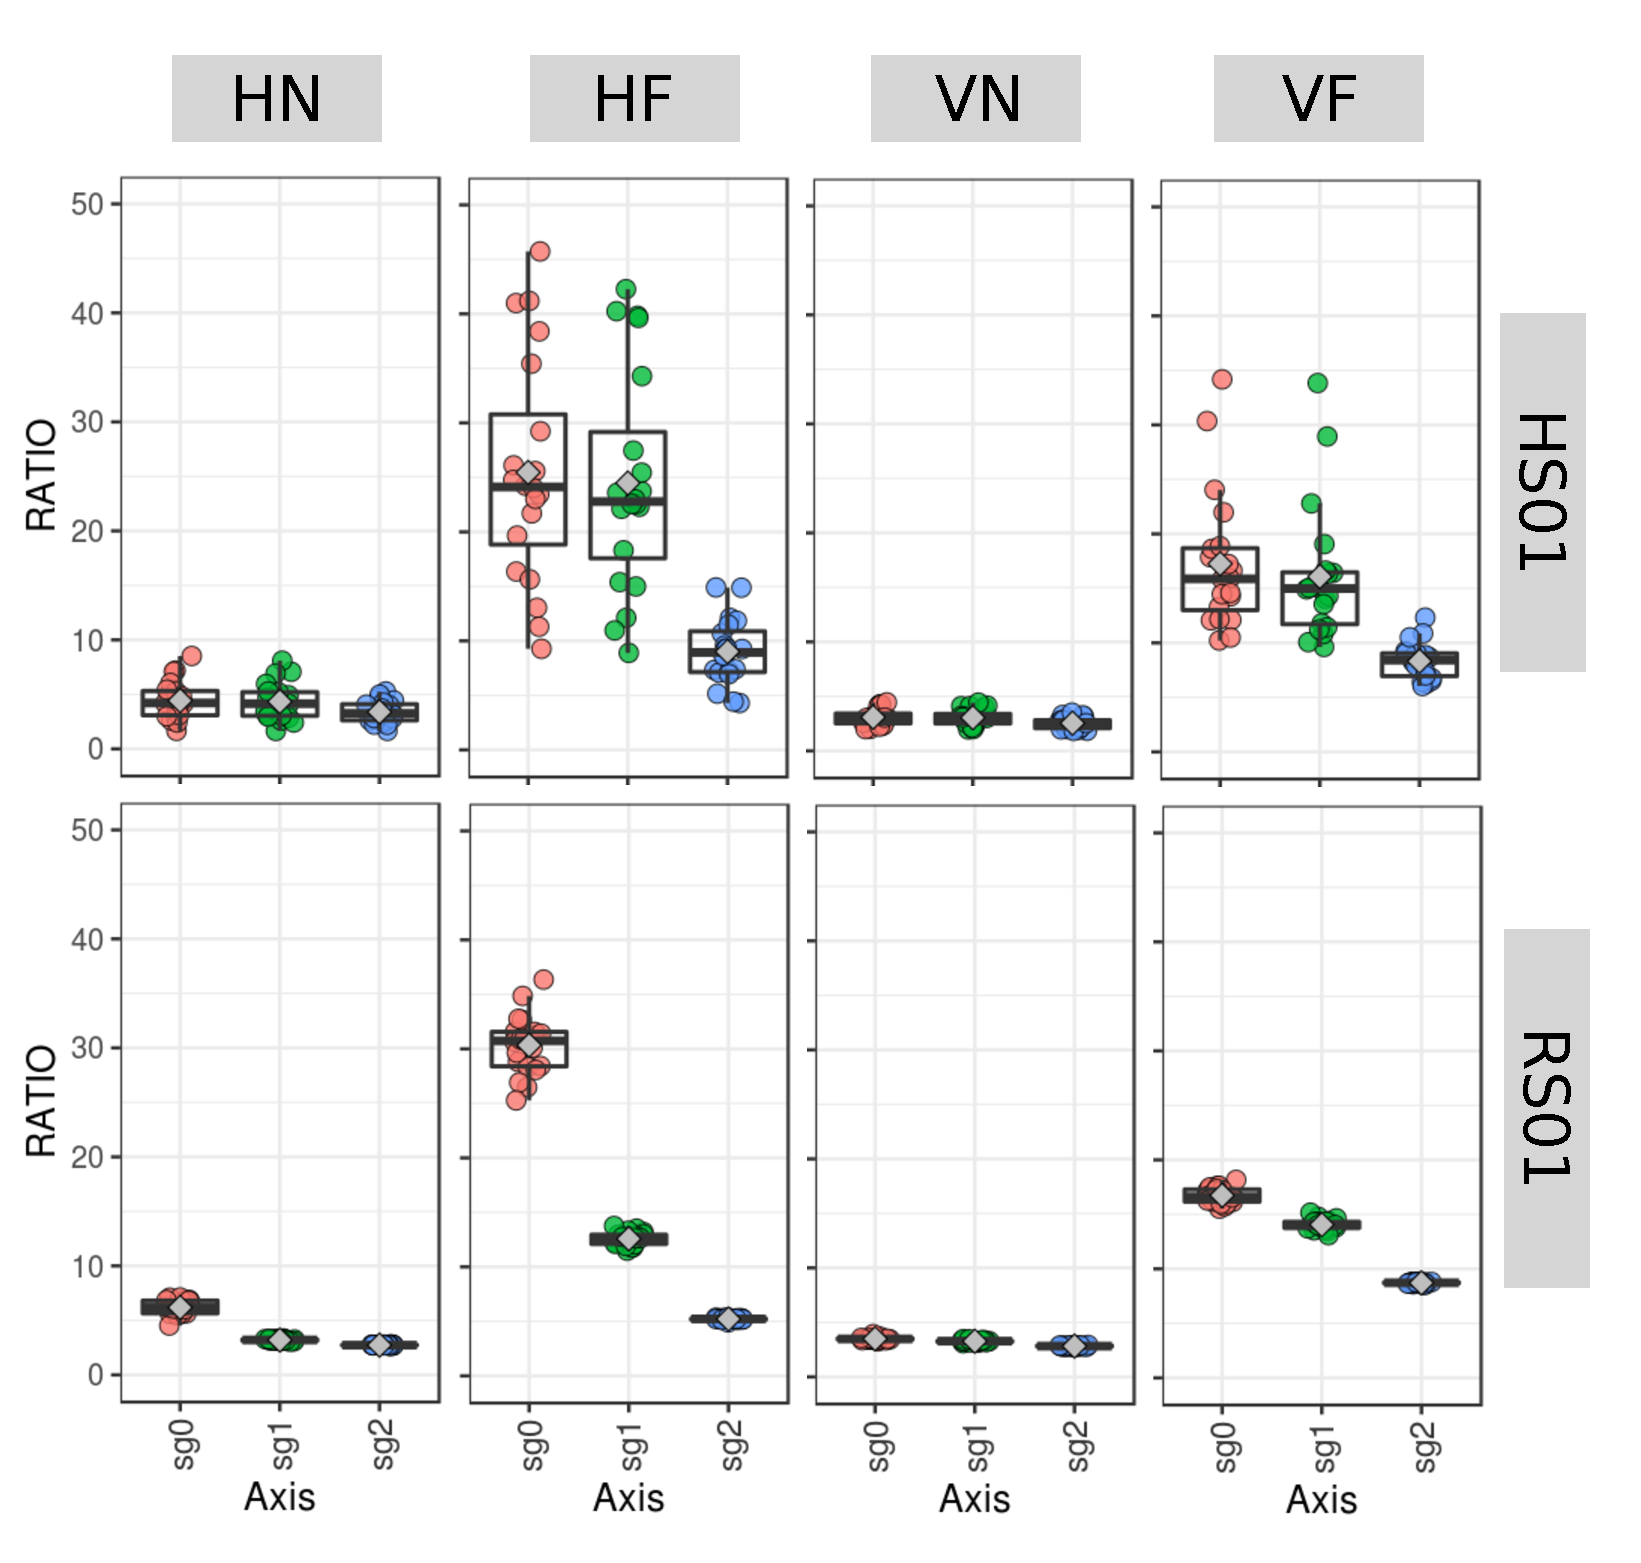
\includegraphics[width=0.6\textwidth]{ratio-bp}
%    \caption{
%	{\bf Box plots for RATIO values.}
%	RATIO (representing dynamic transitions) for 
%	20 participants performing HN, HF, VN and VF movements
%	with sensors HS01, RS01 and three smoothed-normalised 
%	time series (sg0, sg1 and sg2).
%	RATIO values were computed with 
%	embedding parameters $m=6$, $\tau=8$ and $\epsilon=1$.
%	R code to reproduce the figure is available from \cite{hwum2018}.
%        }
%    \label{fig:RATIO}
%\end{figure}
%%%---------------------------------(FIGURE)------------------------------------
%


%\newpage
\subsection*{ENTR values}
Fig. \ref{fig:RQABP}(D) show ENTR values, representing the complexity of 
the structure the time series, for both horizontal and vertical movements.
ENTR values for HS01 sensor show more variation 
(interquartile range around 0.5)
than ENTR values for RS01 sensor which appear 
to be more constant (interquartile range 0.1).
It can also be said that the smoothness of time series affects
each of the axis by an increase of mean values (see gray rhombos).
See Figs~\ref{fig:entr_aH} and \ref{fig:entr_aV} in appendix
\ref{appendix:e:ep}
for more details about individual ENTR values for each participant.
%%%---------------------------------(FIGURE)-------------------------------------
%\begin{figure}
%\centering
%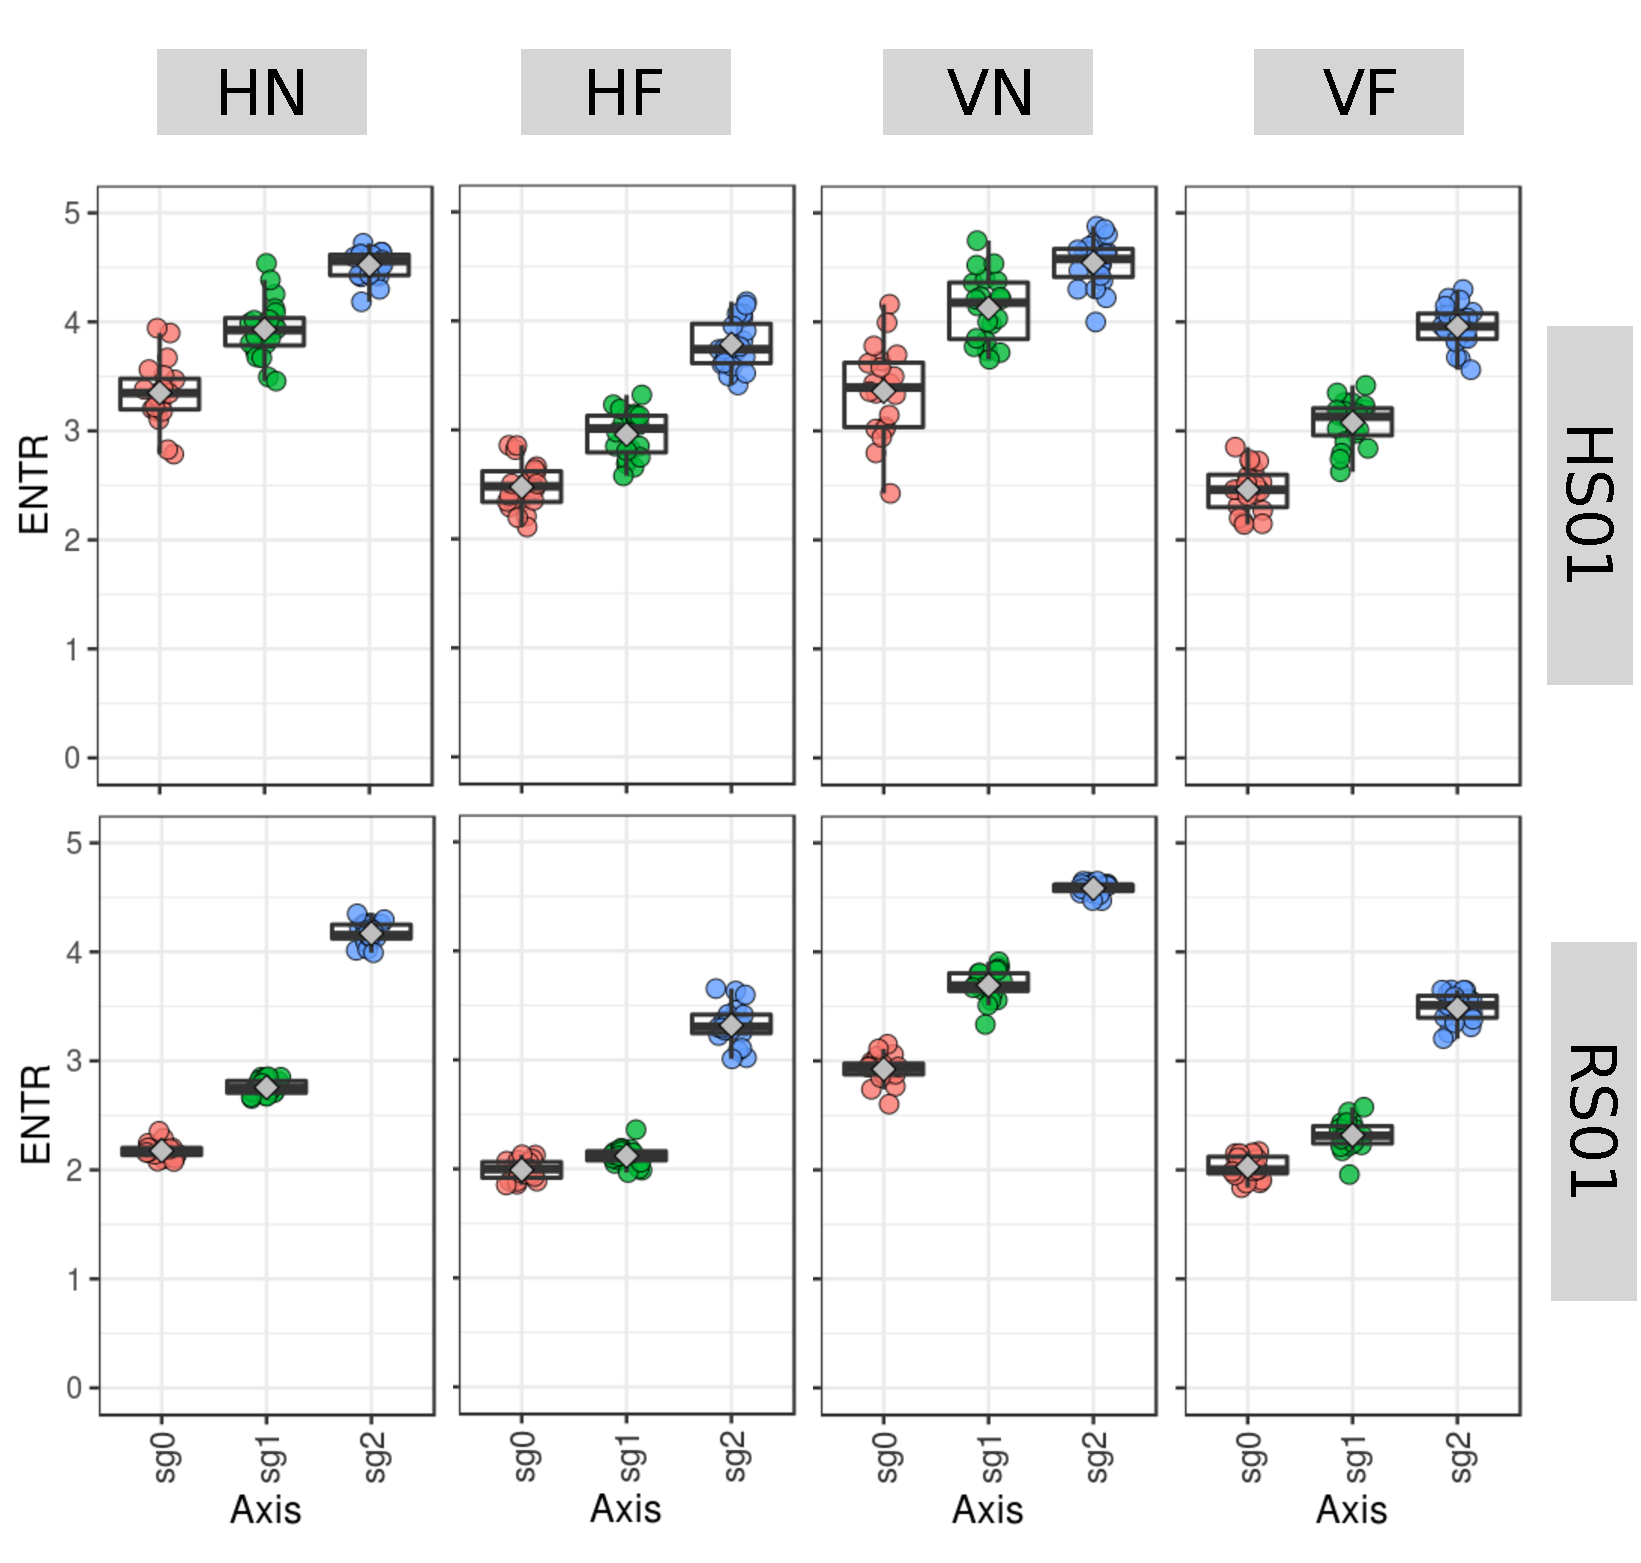
\includegraphics[width=0.6\textwidth]{entr-bp}
%    \caption{
%	{\bf Box plots for ENTR values.}
%    	ENTR values (representing the complexity of the deterministic 
%	structure in time series) for 
%	20 participants performing HN, HF, VN and VF movements
%	with sensors HS01, RS01 and three smoothed-normalised  
%	time series (sg0, sg1 and sg2).
%	ENTR values were computed with 
%	embedding parameters $m=6$, $\tau=8$ and $\epsilon=1$.
%	R code to reproduce the figure is available from \cite{hwum2018}.
%        }
%    \label{fig:ENTR}
%\end{figure}
%%%---------------------------------(FIGURE)------------------------------------
%


%%---------------------------------(FIGURE)-------------------------------------
\begin{figure}
\centering
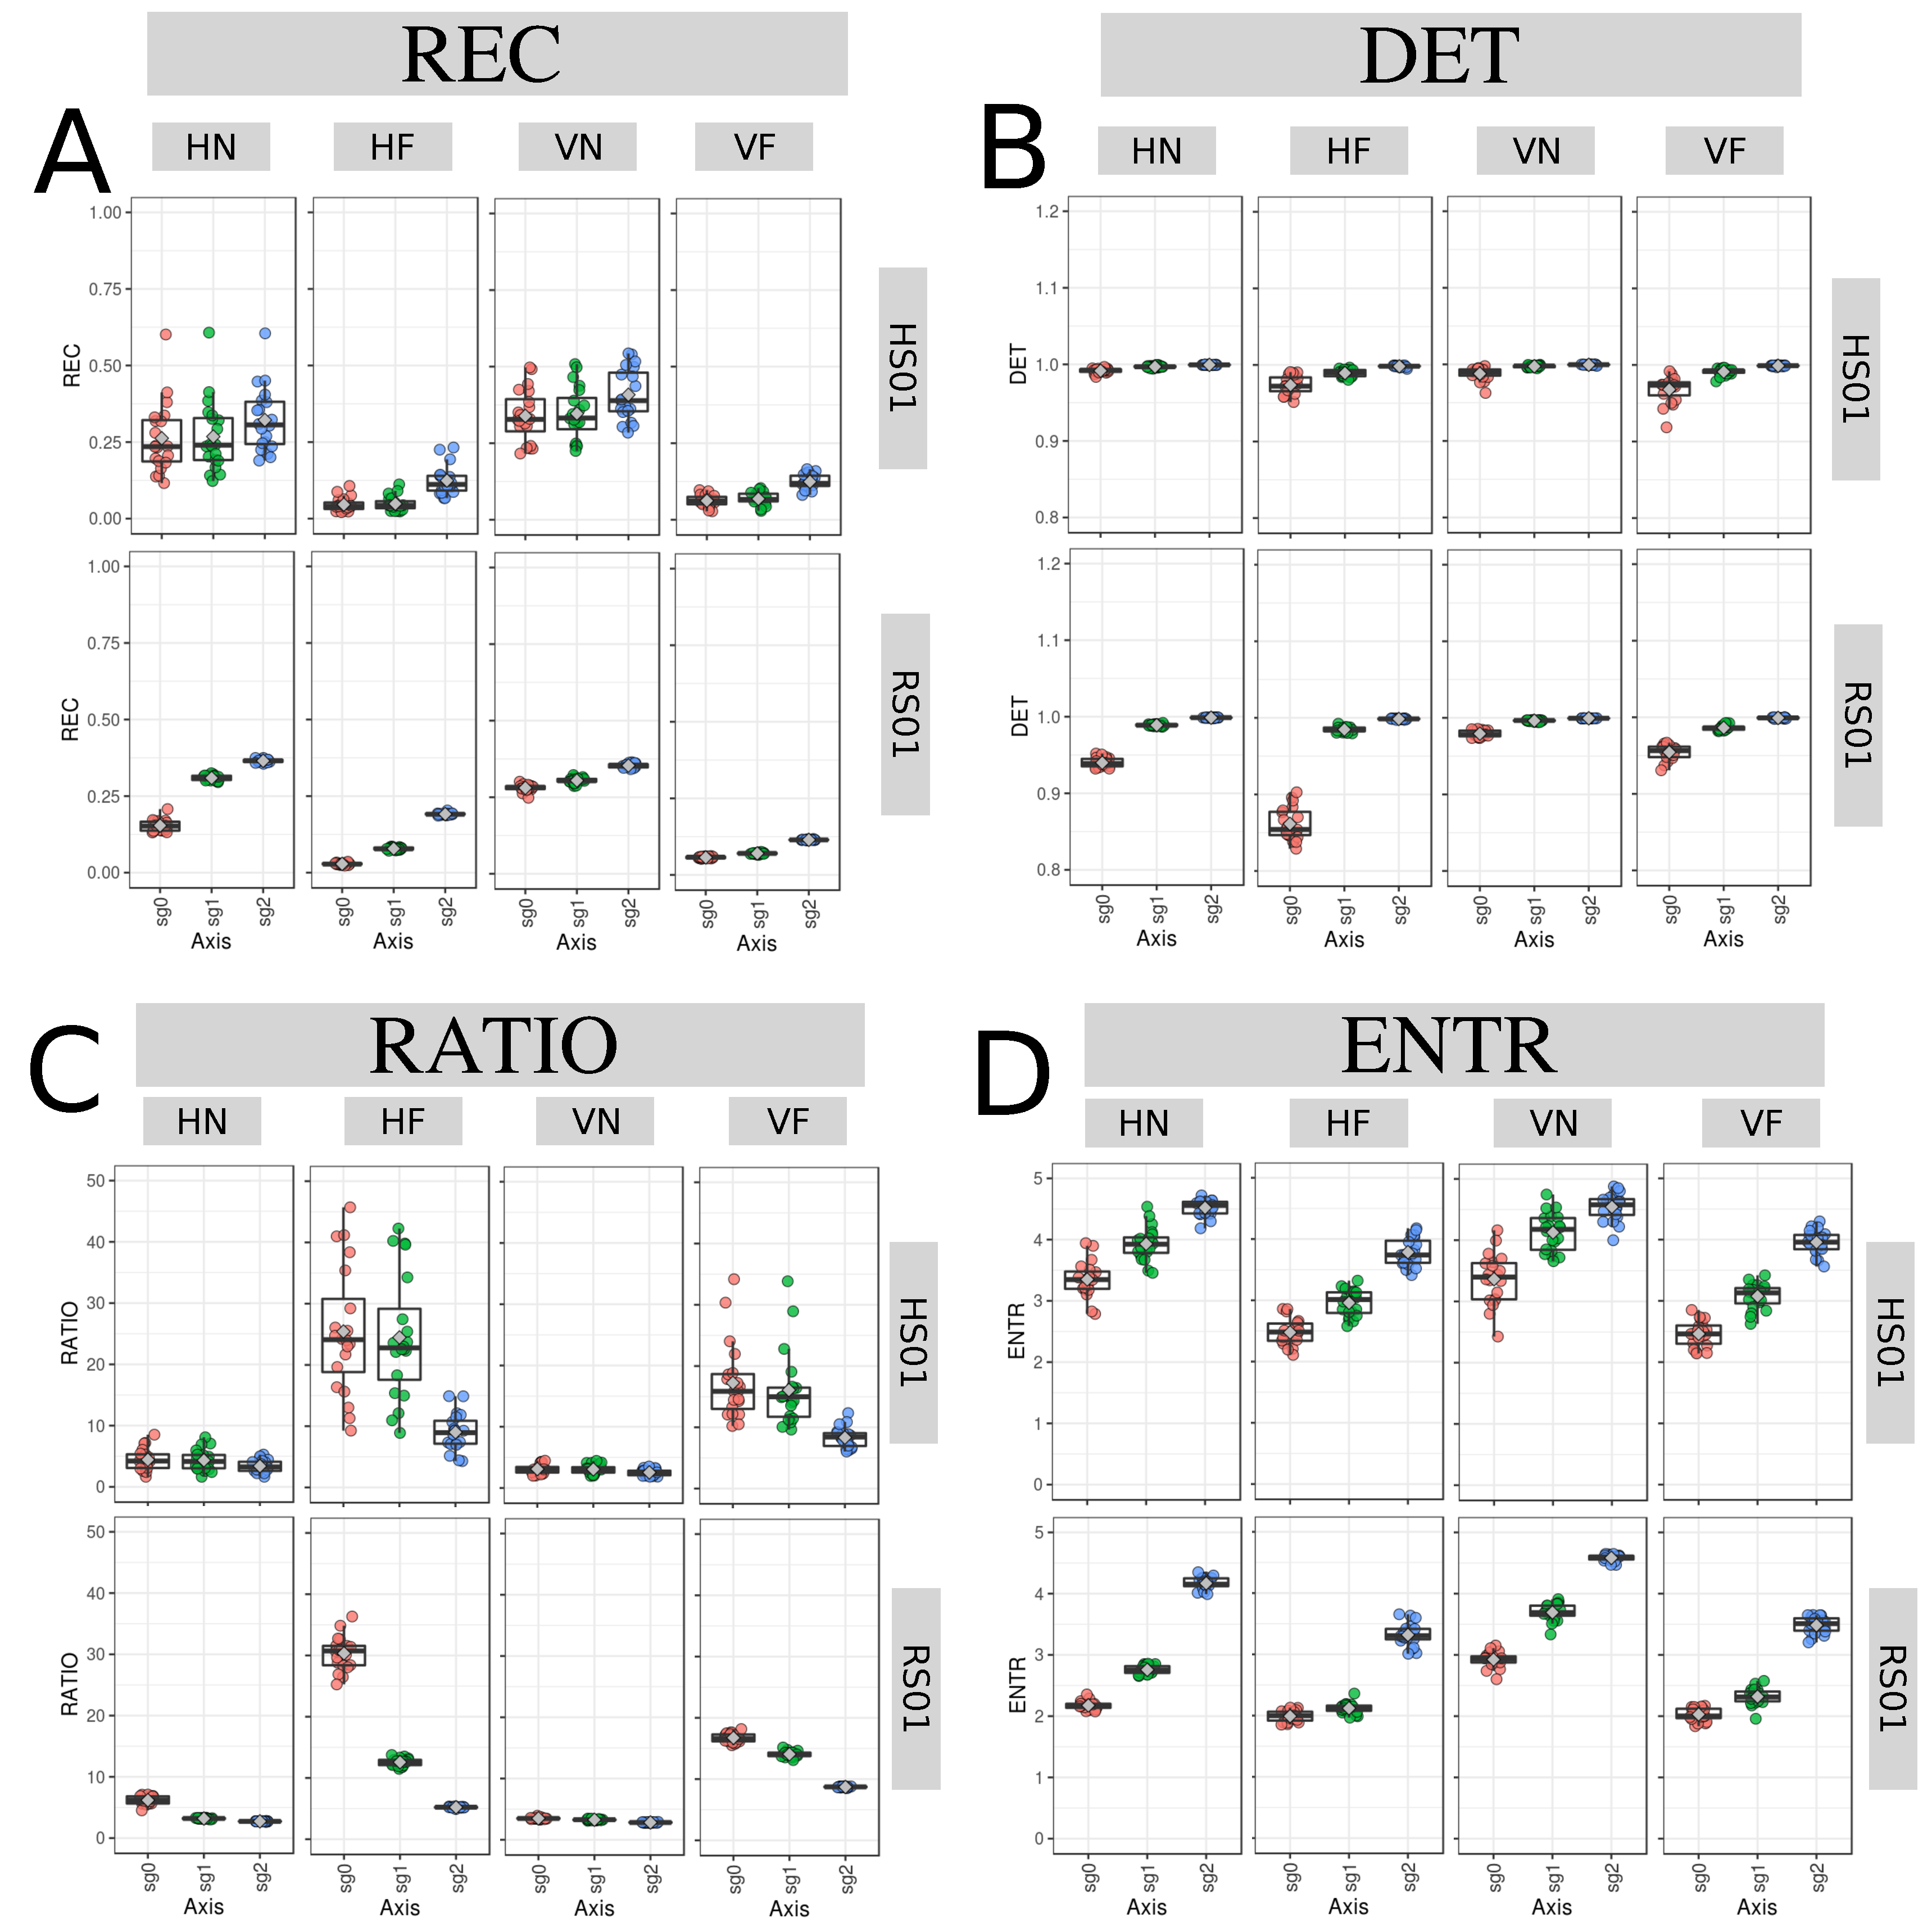
\includegraphics[width=1.0\textwidth]{rqa-bp}
    \caption
	[Box plots for RQA values]{
	{\bf Box plots for RQA values.}
	Box plots of (A) REC, (B) DET, (C) RATIO, and (D) ENTR values 
	for 20 participants performing HN, HF, VN and VF movements
	with sensors HS01, RS01 and three smoothed-normalised  
	time series (sg0, sg1 and sg2).
	RQA values were computed with 
	embedding parameters $m=6$, $\tau=8$ and $\epsilon=1$.
	R code to reproduce the figure is available from \cite{hwum2018}.
        }
    \label{fig:RQABP}
\end{figure}
%%---------------------------------(FIGURE)------------------------------------

















%% \subsection{Effects of different parameters in the computation of 
%% different metrics of RQA.}
%Then we only select the axis AccY and GyroZ as being the axis which show 
%better consistency in the patters for all the posibilities int he time series.
%That was doing visual inspection. It also worthwhile to note that those axis
%represent the majoy energy amothn other axis for both sensors.
%The selection of recurrecne threshold is 1 for HF activites,
%however this should be changed to
%for HN activies.
%With that we also can observe the effect of the seletion 
%of recurrence threshold for different actibities is crucial 
%to have meaninign values in the metrics of RQA.
%% added: Tue 19 Jun 2018

%\section{RQA metrics with different embedding parameters, 
%recurrence thresholds, window lengths, levels of smoothness, and 
%time series structures.}
%

\newpage
\section{Weaknesses and strengths of RQA}
Considering the Section \ref{sec:ws_rqa} regarding 
the weaknesses and strengths of RQA, we computed RQA metrics 
(REC, DET, RATIO and ENTR) and plotted 3D surfaces using an unitary 
increase of pair embedding parameters 
($0 > m \le 10$, $0 > \tau \le 10$) 
and a decimal increase of 0.1 for recurrence thresholds 
($ 0.2 \ge \epsilon \le 3 $) (Fig.~\ref{fig:topo_rqas}). 
Hence, Fig.~\ref{fig:topo_rqas}(A) shows an increase for 
REC values, the percentage of black docs in the RP, 
as the recurrence threshold increase,
while the variation for embedding parameters creates little decrease 
of REC values as the embedding dimensions.
 increase and even a more slighter 
decrements of REC values for the increase of $\tau$.
For the 3D surface of DET values (Fig.~\ref{fig:topo_rqas}(B)), 
representing 
predictability and organisation of the RPs, one can be noted a plateau
for DET values near to 1 for embedding dimension parameters of less 
than 5 and recurrence threshold values of greater than 2 (red surface). 
It can also be observed that the increases of delay embedding made 
the DET values increase so as to make an cascade effect in the surface 
along with the increase of dimension embedding $m$.
For RATIO values, representing dynamic transitions, 
Fig.~\ref{fig:topo_rqas} shows that the 3D surface present 
a plateau (blue surface) of RATIO values 
near to zero for recurrence thresholds greater than 1.0, while 
fluctuations are more evident for recurrence thresholds of less than 1.0,
particularly it can also be noted an increase in the fluctuations of 
RATIO values as the embedding dimension is increasing. 
For ENTR values in Fig.~\ref{fig:topo_rqas}(D), 
representing the complexity of the structures in time series, 
one can be noted that the increase of recurrence threshold is, 
not strictly proportional to the increase of ENTR values. 
It can also be observed in Fig.~\ref{fig:topo_rqas}(D)
that the increase of delay embeddings affects 
little the ENTR values for embedding dimensions of 1, while 
for higher values of embedding dimensions 
there is a decrease of ENTR values, and 
there is a decrease of ENTR values as delay dimension value is increasing.
%---------------------------------(FIGURE)-------------------------------------
\begin{figure}
\centering
\includegraphics[width=1.0\textwidth]{rqas}
    \caption
	[3D surfaces for RQA metrics]{
	{\bf 3D surfaces for RQA metrics.}
	3D surfaces for (A) REC, (B) DET, (C) RATIO and (D) ENTR values 
	with increasing pair of embedding parameters 
	($0 \ge m \le 10$, $0 \ge \tau \le 10$) 
	and recurrence thresholds (  $ 0.2 \ge \epsilon \le 3 $).
	RQA metrics are computed with the time series of participant $p01$ using 
	HS01 sensor, HN activity, sg0zmuvGyroZ axis and 500 samples 
	for window size length.
        R code to reproduce the figure is available from \cite{hwum2018}.
	}
\label{fig:topo_rqas}
\end{figure}
%---------------------------------(FIGURE)------------------------------------


\newpage
\subsection{Sensors and activities}
We also computed 3D surfaces of RQA metrics for different sensors 
and different activities 
(Figs.~\ref{fig:topo_sa_hs01}, \ref{fig:topo_sa_rs01}), where it can 
generally be noted similar 3D surface patterns for RQA metrics as the ones
in Fig. \ref{fig:topo_rqas}. 

The 3D surfaces for REC values (Fig. \ref{fig:topo_sa_hs01}(A))
show slightly differences with regard to vertical or horizontal activities
however there are notable differences for normal and faster velocities, 
specially for the faster movements where the 3D surfaces shown a maximum
REC value for embedding dimension values near to 1 and for recurrence 
thresholds near to 3. 
The 3D surfaces for DET values  
(Fig. \ref{fig:topo_sa_hs01}(B)) and RATIO values 
(Fig. \ref{fig:topo_sa_hs01}(C)) show slightly notable variations across 
the type of activities. 
For 3D surfaces of ENTR values it can be noted a slightly variation for
the surfaces of normal and faster velocities (Fig \ref{fig:topo_sa_hs01}(D)).
%%---------------------------------(FIGURE)-------------------------------------
\begin{figure}
\centering
\includegraphics[width=1.0\textwidth]{sa_hs01}
    \caption
	[3D surfaces of RQA metrics for HS01 sensor]{
	{\bf 3D surfaces of RQA metrics for HS01 sensor.}
	3D surfaces of RQA metrics ((A) REC, (B) DET, (C) RATIO, and (D) ENTR) 
	with increasing embedding parameters and recurrence thresholds 
	are for time series of participant $p01$ for 
	sensors HS01, activities (HN, HF, VN and VF) and 
	sg0zmuvGyroZ axis with 500 samples window size length. 
	R code to reproduce the figure is available from \cite{hwum2018}.
       }
\label{fig:topo_sa_hs01}
\end{figure}
%---------------------------------(FIGURE)-------------------------------------

As similar as Fig \ref{fig:topo_sa_hs01}, the 3D surfaces patters 
for RS01 in Fig \ref{fig:topo_sa_rs01} show the differences between 
the activities performed at normal and faster velocities
specially for REC and ENTR values (Fig \ref{fig:topo_sa_hs01}(A, D)),
while 3D surfaces for DET and RATIO values show slightly variations
(Fig \ref{fig:topo_sa_hs01}(B, C)).
%%---------------------------------(FIGURE)-------------------------------------
\begin{figure}
\centering
\includegraphics[width=1.0\textwidth]{sa_rs01}
    \caption
	[3D surfaces of RQA metrics for RS01 sensor]{
	{\bf 3D surfaces of RQA metrics for RS01 sensor.}
	3D surfaces of RQA metrics ((A) REC, (B) DET, (C) RATIO and (D) ENTR) 
	with increasing embedding parameters and recurrence thresholds 
	are for time series of humanoid robot for 
	sensors RS01, activities (HN, HF, VN and VF) and 
	sg0zmuvGyroZ axis with 500 samples window size length. 
	R code to reproduce the figure is available from \cite{hwum2018}.
       }
\label{fig:topo_sa_rs01}
\end{figure}
%---------------------------------(FIGURE)-------------------------------------








%\newpage
\subsection{Window size}
Figs.~\ref{fig:topo_windows} illustrate 3D surfaces for RQA metrics 
with four window size lengths of 100, 250, 500 and 750 samples.
In general, it can be said that the increase of samples in the time series 
creates 3D surface patterns with better resolution.
%Figs. \ref{fig:topo_windows} 
%---------------------------------(FIGURE)-------------------------------------
\begin{figure}
\centering
\includegraphics[width=1.0\textwidth]{w}
    \caption
	[3D surfaces of RQAs metrics with four window lengths]{
	{\bf 3D surfaces of RQAs metrics with four window lengths.}
	3D surfaces of RQA metrics ((A) REC, (B) DET, (C) RATIO, and (D) ENTR) 
	with increasing embedding 
	parameters and recurrence thresholds for four window 
	lengths (w100, w250, w500 and  w750).
	RQA metrics values are for time series of participant $p01$ 
	using HS01 sensor, HN activity and sg0zmuvGyroZ axis.
	R code to reproduce the figure is available from \cite{hwum2018}.
        }
\label{fig:topo_windows}
\end{figure}
%%---------------------------------(FIGURE)------------------------------------




\newpage
\subsection{Smoothness}
Figs \ref{fig:topo_smoothness} present 3D surfaces of the RQA metrics
considering three levels of smoothness of the time series (sg0, sg1, sg2).
It can then be noted that such smoothness have a direct effect on the 
smoothness of the 3D surfaces.
Especially for dimension embeddings lower than 2 with in REC and ENTR values 
(Fig.~\ref{fig:topo_smoothness}(A, D)).
The 3D surfaces of DET values are smoothed to a degree that the plateau 
(red surface) is increase, while RATIO values appear to be less 
affected to the level of smoothness (Fig.~\ref{fig:topo_smoothness}(C)).
%%---------------------------------(FIGURE)-------------------------------------
\begin{figure}
\centering
\includegraphics[width=1.0\textwidth]{s}
    \caption
	[3D surfaces of RQA metrics with three levels of smoothness]{
	{\bf 3D surfaces of RQA metrics with three levels of smoothness.}
	3D surfaces of RQA metrics ((A) REC, (B) DET, (C) RATIO, and (D) ENTR) 
	with increasing embedding parameters and recurrence thresholds for 
	three levels of smoothness 
	(sg0zmuvGyroZ, sg1zmuvGyroZ and sg1zmuvGyroZ).
	RQA metrics are computed from time series of participant $p01$ using 
	HS01 sensor, HN activity and 500 samples window length.
	R code to reproduce the figure is available from \cite{hwum2018}.
 }
\label{fig:topo_smoothness}
\end{figure}
%%---------------------------------(FIGURE)------------------------------------



%\newpage
\subsection{Participants}
Figs ~\ref{fig:topo_participants} illustrate 3D surfaces of RQA metrics for 
three participants.
It can be noted that differences of the 3D surfaces across participants 
are more notable with REC (Fig.~\ref{fig:topo_participants}(A)) and 
ENTR values (Fig.~\ref{fig:topo_participants}(D)),
while minor differences of 3D surfaces across participants are 
presented in
DET (Fig.~\ref{fig:topo_participants}B)) and 
RATIO vales (Fig.~\ref{fig:topo_participants}(C)).
%%---------------------------------(FIGURE)-------------------------------------
\begin{figure}
\centering
\includegraphics[width=1.0\textwidth]{p}
    \caption
	[3D surfaces of RQA metrics with three participants]{
	{\bf 3D surfaces of RQA metrics with three participants.}
	3D surfaces of RQA metrics ((A) REC, (B) DET, (C) RATIO, and (D) ENTR) 
	for participants $p01$, $p02$ and $p03$ with increasing embedding 
	parameters and recurrence thresholds.
	RQA metrics values are for time series of HS01 sensor, 
	HN activity and 500 samples window length.
	R code to reproduce the figure is available from \cite{hwum2018}.
 }
\label{fig:topo_participants}
\end{figure}
%%---------------------------------(FIGURE)-------------------------------------


\newpage
\subsection{Final remarks}
%	You need to say whether the results are expected and
%	whether different methods agree or contradict each other. 	
Generally, it can be noted the changes for RQA metrics are evident
with both the increase of embedding dimension parameters and the 
recurrence threshold for different structures, window size, 
levels of smoothness of the time series. 
RATIO values present a plateau (blue colour surface) which is independently 
to the source of time series, however there are peaks that change 
differently based on the source of time series for increasing 
embedding parameters  with recurrence threshold less than one.
For DET values, 3D surfaces present a fluctuated surface (red colour)
which slightly differs with the source of time series.
With regards to REC values, 3D surfaces are affected by the velocity
of movements, for instance, surfaces for normal velocity presents 
an increase of REC values as recurrence threshold increase and keeping 
slightly uniform surface changes for the increase of embedding parameters, 
however for faster velocity the 3D surface fluctuations decrease as 
the embedding dimension increase and recurrence thresholds increase.
Similar as the human-image activities  
(see Section \ref{wsRQAhii} in Chapter \ref{chapter5}), 
3D surfaces for ENTR values in human-humanoid interaction  
present changes for any source of time series,
making ENTR values a robust metric to quantify movements variability 
from different time series in human-humanoid activities.




%It is also important to highlight that the patterns in the 3D 
%surfaces of the RQA metrics (REC, DET, RADIO and ENTR) 
%(Fig \ref{fig:topo_rqas}) are certainly similar to its corresponded
%metrics for the different characteristics of the time series  
%(Figs. \ref{fig:topo_sa_hs01}, \ref{fig:topo_sa_rs01}, 
%\ref{fig:topo_windows}, \ref{fig:topo_smoothness}, 
%\ref{fig:topo_participants}).




 %Quantifying Human-Humanoid Imitation Activities


%%*******************************************************************************
%****************************** Sixth Chapter *********************************
%*******************************************************************************

\chapter{Conclusion}

%% **************************** Define Graphics Path **************************
%\ifpdf
%    \graphicspath{{chapter7/figs/raster/}{chapter7/figs/PDF/}{chapter7/figs/}}
%\else
%    \graphicspath{{chapter7/figs/vector/}{chapter7/figs/}}
%\fi
%


%%**************************** %Broad Purpose  **********************************
%\section*{Summary and broad purpose of the chapter}
%* How long (number of words)?
%* Deadline
%* What have you got?


\section{Discussion}


\subsection{ami}


Further investigation is required for the selection of the threshold 
in the $E_1(m)$, as the selection of the threshold in this work is base on 
no particular method but visual inspection.

Additionally, we observe two additional negative aspects of the use of the 
False Nearest Neighbour method \cite{Cao1997}: 
(i) %the main requirements for the use of Cao's method are 
from the input time series, a value to set up the maximum embedding dimension 
and delay embedding, Cao's algorithm computes $E_1(m)$ and $E_2(m)$, however
when the values for $E_1(m)$ stop changing, a threshold should be 
defined in order to obtain the minimum embedding dimension $m_0$, and
(ii) Cao's method computes different embedding dimensions 
when using different window lengths for the time series as shown in chapter 
\ref{chapter5} and \ref{chapter6}.



\subsection{other}

It is evidently that time series from different sources (participants, movements, axis type, 
window length or levels of smoothness) presents visual differences for 
embedding parameters and therefore for RRSs. For which, the selection of embedding parameters 
was our first challenge where we computed embedding parameters for each time series and 
then computed a sample mean over all time series 
in order to get two embedding parameters to compute all RSSs with its corresponded type of movement.
Then we found that the quantification of variability with regard to the shape 
of the trajectories in RSSs requires more investigation since our original proposed method 
base on euclidean metric failed to quantify those trajectories. Specially, for trajectories 
which were not well unfolded. With that in mind, we proceed to take advantage of 
four RQA metrics (REC, DET, RATIO and ENTR) in order to avoid any subjective interpretations 
or personal bias with regard to the evolution of the trajectories in RSSs.


\subsection{RQA metrics with fixed parameters}
Considering that RQA metrics were computed with fixed embedding parameters 
($m=6$ and $\tau=8$) and recurrence thresholds ($\epsilon=1$), we found the following.
REC values, which represents the \% of black points in the RPs, were more affected with 
and increase in normal speed movements (HN and VN) than faster movements (HF and VF)  
for the sensor attached to the participants (HS01). Such decrease of REC values 
from normal speed to faster speed movements is also presented in data from sensor 
attached to the robot (RS01), and little can be said with regard to the dynamics
of the time series coming from RS01. 
Similarly, DET values, representing predictability and organisation in the RPs, 
present little variation in the any of the time series where little can be said.
In contrast, RATIO values, which represent dynamic transitions, were more 
variable for faster movements (HF and VF) than normal speed movements (HN and VN) 
with sensors attached to the participants (HS01).
For data coming from sensors attached to the robot (RS01), RATIO values
from horizontal movements (HN, HF) appear to vary more than 
values coming from vertical movmentes (VN, VF).
With that, it can be said that RATIO values can represent a bit better
than REC or DET metrics for the variability of imitation activities in each of the conditions
for time series.
In the same way, ENTR values for HN were higher than values for HF
and ENTR values varied more for sensor attached to participants 
than ENTR values for sensors of the robot. It is evidently that 
the higher the entropy the more complex the dynamics are, 
however, ENTR values for HN appear a bit higher than HF values, 
for which we believe this happens because of the structure the time series
which appear more complex for HN than  HF movements which presented a 
more consistence repetition.

We observed that some RQA metrics are affected by the smoothness of data.
For which, we also explored the effect of smoothness of raw-normalised data 
where, for example, REC and DET values were not affected by the smoothness 
of data since these seemed to be constants. However, for RATIO values, 
the effect of smoothness can be noticed with a slight decrease of amplitude 
in any of the time series conditions which is also presented with ENTR values.


\subsection{RQA metrics with different parameters}
Patterns in RPs and metrics for RQA are independent of embedding dimension parameters \cite{iwanski1998},
however, that is not the case when using different recurrence thresholds. Such changes of 
recurrence threshold values can modify the patterns in RPs and therefore the values of RQA metrics. 
We therefore computed 3D surfaces to explore the sensibility and robustness of 
embedding parameters and recurrence threshold in RQA  metrics. 
Following the same methodology of computing 3D surfaces, we also considered variation 
of window length size to present RQA metrics dependencies with embedding parameters, 
recurrence thresholds and window length size.





\section{Conclusions}
We conclude that using a different level of smoothness for time series help us 
to visualise and to quantify the variation of movements between participants 
using RSSs, RPs and RQA. Also, it is important to mention that some RQA's metrics 
(e.g. DET and  ENTR) are more robust to the effect of smoothness of time series.

Althought our our experiment is limited to twenty healthy right-handed participants 
of a range age of mean 19.8 SD=1.39, RQA metrics can quantify human movement 
variability. With that in mind, we conclude that qunatification of human-humanoid
imitation activities is possible for participants of different ages, state of health 
and anthropomorphic features.


%
%Such understanding and measurement of movement variability using
%cheap wearable inertial sensors lead us to have a more intuitive selection of parameters
%to reconstruct the state spaces and to create meaningful interpretations
%of the recurrence plots and the results of the metrics with recurrence quantification 
%analysis. 
%

In general, activity type, window length and structure of the time series 
affects the values of the metrics of RQA for which certain RQA metrics 
are better to describe determined type of movement.
Using determined RQA metrics depends on what one want to quantify, for instance, 
one can find predicability, organisation of the RPs, dynamics transitions, 
or complexity and determinism.


%
%However, we believe that further investigation is required to find the 
%right balance between the level of smoothness of the signal
%and defining what is the aim of RQA where 
%its representations using RSS, RP and RQA.
%Specially, where the level of smoothness does not affect 
%the variation of each of the movements quantification. 
%%We can also conclude that finding the right balance between 
%%smoothness and the raw data to capture movement variability is 
%%a still a problem that has many avenues for exploration.
%

Similarly, such differences in time series created differences in each of the 
RQA metrics, for instance, RATIO and ENTR are helpful to distinguish 
differences in any of the categories of the time series (sensor, activity, 
level of smoothness and number of participant), however for certain time series 
(data from the sensor attached to the robot) seemed to have little variations 
between each of the participants. The latter phenomena was in a way evidently
as robot degrees of freedom did not allow it to move with a wide range of variability. 





\section{Future Work}

\subsection{Inertial Sensors}
To have more fundamental understating of nature of signals collected through 
inertial sensors in the context of human-robot interaction, we are considering to apply 
derivates to the acceleration data. We can then explore the jerkiness of movements 
and therefore the nature of arm movements which typically have minimum jerk \cite{flash1985},
its relationship with different body parts \cite{devries1982, mori2012} or
the application of higher derivatives of displacement with respect time 
such as snap, crackle and pop \cite{eager2016}.



\subsection{RQA}
Having presented our results with RQA metrics, we believe that further investigation 
is required to have more robust metrics. For example, Marwan et al. \cite{marwan2007, marwan2015} 
reviewed different aspects to compute RPs using different criteria for neighbours, 
different norms ( $L_{1-norm}$, $L_{2-norm}$, or $L_{\infty-norm}$ ) or 
different methods to select the recurrence threshold $\epsilon$, such as using certain percentage 
of the signal \cite{letellier2006}, the amount of noise or using a factor based 
on the standard deviation of the observational noise among many others \cite{marwan2007}.











%%**************************** %Summary of the Argument  **********************************
%\section[Conclusion]{Summary of Argument}
%
%\section[Future Work]{Implications}
%

In this work, an experiment is performed in the context of human-humanoid imitation activity
to test nonlinear dynamics methods to quantify human movement variability. 
The presented results that illustrate the potential of nonlinear dynamics tools 
by providing a balanced review of positive and negatives aspects of each 
technique to quantitatively and qualitatively measure movement variability.

With regards to the visual inspection and understanding of the patters
for reconstructed state spaces and recurrence plots,
it can also be concluded that the performance of such tools is subjective 
since biased personal data interpretation might be provided.
Hence, without any bias, RQA metrics (REC, DET, RATIO and ENTR) help us to show 
such differences of movement variability for difference categories 
of the time series (participants, movements, axis type, window length or levels of smoothness).
Furthermore, it was noticed that each of the metrics of RQA show the differences 
but particularly the metrics of RATIO and ENTR are helpful to distinguish 
the differences in each of the categories of the time series.
%We therefore collecte data series using inertial sensors and we smooth
%the signals to see its graphical effects and also in the metrics.
%With that in mind, embedding values to create the reconstructe state spaces
%and theferfore its recurrence plots. By doing that, we saw that visually
%each of the particpants in each of the conditions for movemetns and 
%levels of smootheness of the signlas are evicently differently, therefore
%the challenge for us were to have a quantitavely method for each of the 
%difference in the patterns for RP for which we took the adnavce of the use 
%of Recurrene Qantification Analysis which show important results 
%that help us to quantify the variality between particpants and between 
%movments. We esentially noticed that each of the metrics of RQA
%(REC, DET, RATIO and ENTR) can shown differences but specially RATIO
%and ENTR are helpful to distinguis the differences in each of the movments.
%%Tue 19 Jun 12:21:56 BST 2018

Although RPs and metrics for RQA are independent of embedding dimension \cite{iwanski1998},
it was found that recurrence threshold values can modify the results for both RPs and RQA.
This work has carried out experiments on different activities in which 
the sensor's axis was representative of difference of structures in the time series.
Hence, further investigation is required.
In a similar experiment carried out by \cite{letellier2006}, an equation was defined following 
several trials for the selection of recurrence threshold. 
This equation was used to determine the recurrence plot 
($\sqrt{m_0} \times$ 10\% of the fluctuations of the time series).



%With that in mind we did the same for the selection 
%of the right threshold for our particular problem where we first select 
%a threhold of 1 for all the signals however, these value is not
%appropriate for both activites, as for example the HN and HF 
%show sometimes white RP which should not be the case if 
%we select a right emedding threshodl.
%However, we have found the following problems
%% ENT
%For RQA the window effect is crucial for each of the metrics
%so for example, ENT values for HN are higher and HF are lower
%meaming that these are less comples than HN values, we believe
%that happens because of the lnght windows. Althought,
%these values apper to be more complex for HF, 
%the values in HN have less repetutions of tmovments 
%which is the reason to have those differences in ENT values.
%%#added Mon 18 Jun 12:32:55 BST 2018
%For, RATIO values apper to have more variations across particpants
%for which we believe that RATIO values represent a bit better
%the variatbiltuy of imitation activitivies and also the 
%movment variaiblaituy that is created in this experiemnt.
%%added: Mon 18 Jun 14:06:19 BST 2018
%and for ENTR values show little variation across partipants and these
%are generally higher for HN than HF movmentes in each of the 
%smothed signals. We believe that ENTR values are affected
%by the windown lenght so as to say that HN values 
%represent more complex structures than those coming from 
%HF values.
%%added: Mon 18 Jun 14:17:27 BST 2018

It was also found that using a different levels of smoothness
for time series helps to visualise the variations of movements 
between participants using RSSs, RPs and RQA. Also, it is important to mention 
that some RQA's metrics (e.g. DET and  ENTR) are more robust 
to the effect of smoothness of time series.
However, we believe that further investigation is required to find the 
right balance between the level of smoothness of the signal
and its representations using RSS, RP and RQA.
Particularly, where the level of smoothness does not affect 
the variation of each of the movements' quantification.
%which is similar to the raw normalised data. Also the raw normalised
%data can show more details information of for the movement, however
%these are not lost as the time series is smoothed.
%We can also conclude that finding the right balance between 
%smoothness and the raw data to capture movement variability is 
%a still a problem that has many avenues for exploration.
%
%other variables affect the data from the sensors such as  
%temperature of the sensor processing, variation of the sampling
%rate which esentially are involved in the quqlity of the data.
% 
%We only create two to four levels of smoothness using the 
%savtiktzy-golay filter with same degree for different filter lenght
%for which we were able to see the differences in each of the 
%nonlinear dyamics tools. 
%We also propose four window size lenght  to see the effects
%in the nonlinear dynamics tools.
%%add more conclusions about the reuslts of the changes in rss, rp and rqa
%%as these parameters chagne.
%\subsection{Perception of speed}

It is important to mention that while performing the experiments 
with different arm movements speeds (e.g. normal and faster), it was 
realised that participants perceive speed in different ways.
For instance, some participants considered a normal speed movement 
as slow speed movement and some others considered a 
slow speed movement as being performed in normal speed. 
That sheds light of the need for future work to understand 
how each participant perceive body movement speed differently.
%which we hipothese that the differences in perception of speed
%are related to the background of each person, for exmaple,
%person who have receive musical training in their infancy
%are more aware of their body movemnets [add reference]
%It would also be intersting to ask participants
%to move in three different speeds withouth any aconstration in order to 
%capture the natural movements for slow, normal and faster speed 
%arm  movements.
It should also be highlighted that the experiment is limited to twenty healthy 
right-handed participants of an age range of mean 19.8 SD=1.39, 
for which participants of different ages, state of health and anthropomorphic features
would create more richness in the dataset of time series.
%to understand and quantify movement variability using nonlinear dynamics tools.
%With regard to the humanoid movements, I realise that
%it is imporant to program the robot with using the same speed
%and also considering movements that the robot can perform, 
%so for example when the speed is a bit higher the 
%robot's movements tend to be jerky.
%Also create uniform speeds of each of the movments, 
%I realise the the horizontal and vertical movements in 
%normal and faster speed were different which might 
%affect the perception of people movements.
%

%FUTURE WORK

%INERTIAL SENSORS
Additionally, a more meaningful understating
of the nature of the signals collected with inertial sensors
is required in cases where by derivate the acceleration data,
jerk movements and its relationship with different 
body parts can be explored \cite{devries1982, mori2012} and its nature of 
arm movements considered to have typically minimum jerk \cite{flash1985}.
%THIS IS MEANINGLESS AND DOES NOT FIT IN THIS PARAGRAPH AT ALL
% which can interpreted as the change in acceleration
%or jounce which is the derivatives of jerk and it is know to measure 
%the change of jerk.
%%%%Tue  8 May 17:44:36 BST 2018
%
%More interesting problems can be explored as the relationshop 
%for how rapid or slowly for arm and legs we perform as we grow up  
%\cite{devries1982, mori2012} and its nature o
%and in different activitues wher for example for human 
%reaching movmetnes, theser present typically minimum jerk 
%%\cite{Flash Hogan (1985).}
%and fundamentally how it can be qunatified using jerk and jounce.
%%added: Tue 19 Jun 13:16:02 BST 2018
%




%
%
%%%%%%%%%%%%%%%%%%%%%%%%%%%%%%%%
%%% Mon 14 May 13:15:33 BST 2018
%
%Having better understanding of RP, 
%requires to read the marvan2008: 
%%@ARTICLE{2008EPJST.164....3M,
%%   author = {{Marwan}, N.},
%%    title = "{A historical review of recurrence plots}",
%%  journal = {European Physical Journal Special Topics},
%%archivePrefix = "arXiv",
%%   eprint = {1709.09971},
%%     year = 2008,
%%    month = oct,
%%   volume = 164,
%%    pages = {3-12},
%%      doi = {10.1140/epjst/e2008-00829-1},
%%   adsurl = {http://adsabs.harvard.edu/abs/2008EPJST.164....3M},
%%  adsnote = {Provided by the SAO/NASA Astrophysics Data System}
%%}
%%
%
%
%


%%%%%%%%%%%%%%%%%%%%%%%%%%%%%%%
%%%Thu 10 May 13:10:45 BST 2018
%Considering the work of \cite{shoaib2016},
%futher experimets can be permoed with the combination of linear acceleartion
%n, which is obtained by removing acceleration due to 
%gravity from the accelerometer, with accelerometer and gyroscope.
%"the acceleration due to gravity is useful for differentiating static postures
%such as sitting and standing" but it is sensitive to changes in sensor orientation
%and body position.
%
%[Florentino-Liano, B.; O’Mahony, N.; Artés-Rodríguez, A. Human activity recognition using inertial sensors
%with invariance to sensor orientation. In Proceedings of the 2012 3rd IEEE International Workshop on
%Cognitive Information Processing (CIP), Baiona, Spain, 28–30 May 2012; pp. 1–6.]
%%



%\subsection*{Perception of speed}
%While performing the experiments in the human-humanoid imitation activies with 
%different arm movements speeds (e.g. normal and faster), we realised that 
%participants perceive speed in different way, for instance, some participants 
%might consider a normal speed movement as slow speed movement and some other
%the viceversa case. That led us to our future work, where further experimentation is required 
%to understand how each participant perceive body movement speed differently.
%%which we hipothese that the differences in perception of speed
%%are related to the background of each person, for exmaple,
%%person who have receive musical training in their infancy
%%are more aware of their body movemnets [add reference]
%%It would also be intersting to ask participants
%%to move in three different speeds withouth any aconstration in order to 
%%capture the natural movements for slow, normal and faster speed 
%%arm  movements. 
%% added: Tue 17 Jul 19:26:05 BST 2018



%It is also important to note that we considered the use of normalised raw 
%time series from the inertial sensors, however, performing the reconstructed state space 
%require a dimensionality recudtion using PCA where another noramlisation of data 
%is performed for such dimensioanlity reduction.
%In constrast, computing RPs and RQAs require the creating of an UTDE matrix, 
%however, there is no extra normalisation than the normalised raw data of the input 
%of RPs and RQAs.
%added: Fri 20 Jul 00:48:14 BST 2018

%
%FUTURE WORK FOR RQA
%Similarly, Iwansky et al. \cite{iwanski1998} pointed out that two dissimilar RPs: 
%one from the R\"{o}ssler system and the other one from a sine-wave signal of varying 
%period have got equal values of REC (2.1\%) and near-equal values of 
%DET (42.9\%, 45.8\%, respectively). Where we believe other RQA's can be more 
%realiable for certain source of the time series.
%added: Fri 20 Jul 01:12:50 BST 2018
%




%HUMAN_HUMANOID IMTAITON APPLICAITONS
%The work of \cite{guneysu2014} raised an important point of not considering 
%latency of motions for velocity or symmetry of motion which can be used as 
%indicators of attention deficit, boredom, or lack of perception.
%Tue 31 Jul 19:22:29 BST 2018



% Investigate \section{Group Activity in Human-Humanoid Imitation}
%added Thu  2 Aug 21:56:20 BST 2018





%%**************************** %Zero Section  ***********************************
%\chapter{Automatic Classification}
%\section{Convolutional Neural Networks (CNN)}
%\lipsum[0-4]
%
%\section{CNN Using time-series}
%

%added Thu  2 Aug 23:40:14 BST 2018



FUTURE WORK WITH
\subsection{Other methodologies for state space reconstruction.}
In addition to the Uniform Time-Delay Embedding method, other methods have 
recently been investigated to perform state space reconstruction.
For instance, (i) the nonuniform time-delay embedding methodology  
where the consecutive delayed copies of $\{ \boldsymbol{x}_n  \} $ are not
equidistant. Such method has been probed to create better representations 
of the dynamics of the state space to analyse, for instance, 
quasiperiodic and multiple time-scale time series over the conventional 
uniform time-delay embedding algorithm \citep{pecora2007, uzal2011, 
Quintana-Duque2012, Quintana-Duque2013, Quintana-Duque2016}, and
(ii) Uniform 2 time-delay embedding method which takes advantage 
of finding an embedding window instead of the traditional method 
of finding the embedding parameters separately \citep{gomezgarcia2014}.
In general, Uniform 2 time-delay embedding method computes $m$ with 
False Nearest Neighbour (FNN) algorithm and $\tau$ is computed as 
$\tau= d_w / (m-1)$, where $d_w$ is given by the minimisation of the 
Minimum Description Length \citep{small2004}.
However, these methods are out of the scope of the thesis but it is 
important to refer readers to those references for further investigations  
in this regard.


Future work with 
\subsection{Advanced quantifications}
In addition to the previous variables for recurrence quantification, 
\cite{marwan2007, marwan2015} investigated further quantification methodologies 
of the RP based on complex networks statics, calculation of dynamic invariants, 
study of the intermittency in the systems, applying different windowing techniques or the study of bivariate recurrence analysis for correlations, 
couplings, coupling directions or synchronisation between dynamical systems.



Future work with AMI
%Similarly as Cao's algorithm negatives, AMI's algorithm is not an
%exception for negatives, which are worthwhile to mention for further 
%investigations.
It is not clear why the choose of the first minimum of the AMI is the 
minimum delay embedding parameter \citep{kantz2003} or why the probability 
distribution of the AMI function is computed with the use of histograms 
which depends on a heuristic choice of number of bins for AMI partitioning 
\citep{garcia2005e71}. Further, "the method is proposed for two dimensional 
reconstructions and then extended to be used in a multidimensional case 
which is not necessarily hold in higher dimensions" 
\citep[p. 156]{gomezgarcia2014}.



 %Conclusion and Future Work



%%********************************** Appendices *****************************
\begin{appendices} % Using appendices environment for more functunality
%%!TEX root = ../thesis.tex
% ******************************* Thesis Appendix A ****************************
\chapter{Inertial Measurement Units}



A list of description for Inertial Measurement Units which includes
* on-board processing?
* embedded sensor fusion
* Sample rate variation and what does it depend on?
* What data does it send? Acceleration output?/calibrated data?
* What rate did they sample when sending information on Multiple



\section{Muse}
The sample rate for muse sensors goes from 25, 50, 100, 150, and 200 Hz and it
depends from 8MHz oscillator which has \%0.5 frequency tolerance and
$\pm$ 0.2 \% frequency shift by temperature -40$^{\circ}$C and 80$^{\circ}$C
and $\pm$ 0.1 \% frequency aging.

\subsection{TODO: present an explanation for the use of time syscronisation in the
wireless network}

\subsection{TODO: Present a simple explanation regarding the use of MUSE sensors!}

\subsection{Accelerometer}
\subsection{Angular rate gyroscope}
\subsection{Magnetometer}
\subsection{The IMU signal}
\subsection{Kinematic Parameters}

\subsection{System set-up}
\subsection{System calibration}
\subsection{Output}

read Roetenberg2013 for a better structure of the information for the muse section.

% @TECHREPORT{Roetenberg09xsensmvn:,
%     author = {Daniel Roetenberg and Henk Luinge and Per Slycke},
%     title = {Xsens mvn: full 6dof human motion tracking using miniature inertial sensors. Xsens Motion Technologies BV},
%     institution = {},
%     year = {2009}
% }



\section{Razor IMU 9dof}

\section{Axivity Sensors}


WAX9 Unit price is 149 pounds.
It doesnt provide a kinematic chain and there is no online magnetometer calibration.

POSITIVES.
Many reserach works has been uused the WAX sensros in many publications:
[http://axivity.com/publications]

2009, 1 paper
2011, 4 papers
2012, 4 papers
2013, 19 papers
2014, 10 papers
2015, 32 papers
2016, 48 papers
2017, September, 19 papers



NEGATIVES. There is no validation test against any optical sensor or xsens sensors



% @article{FENG201711,
% title = "Comparison of tri-axial accelerometers step-count accuracy in slow walking conditions",
% journal = "Gait & Posture",
% volume = "53",
% number = "",
% pages = "11 - 16",
% year = "2017",
% note = "",
% issn = "0966-6362",
% doi = "http://dx.doi.org/10.1016/j.gaitpost.2016.12.014",
% url = "http://www.sciencedirect.com/science/article/pii/S0966636216307020",
% author = "Yuanyuan Feng and Christopher K. Wong and Vandana Janeja and Ravi Kuber and Helena M. Mentis",
% keywords = "Accelerometers",
% keywords = "Step count",
% keywords = "Device comparison",
% keywords = "Piecewise Aggregate Approximation"
% }




\section{Xsens}


accurate and drift free orientation
the update rate varies with regard to the number of trackers
1MTw 120Hz
2MTw 120Hz
9MTw 100Hz
10MTw 80Hz
20MTw 60Hz

MTw Awinda DK Lite (E 740) contains:
MTw Awinda motion trackers; the awinda USB dongle; and USB charging cable.
(E 400) per extra tracker.

The price for 6 motion trackers is E 4390




% @TECHREPORT{Roetenberg09xsensmvn:,
%     author = {Daniel Roetenberg and Henk Luinge and Per Slycke},
%     title = {Xsens mvn: full 6dof human motion tracking using miniature inertial sensors. Xsens Motion Technologies BV},
%     institution = {},
%     year = {2009}
% }


\section*{Benchmark}

\subsection*{Shimmer3 (Dublin, Ireland)}


BtStream firmware program is used for shimmer configuration
and data capture over Bluetooth.
The Shimmer unit is within Bluetooth range of the PC (<12m approximately).

rechargeable Lithium Polymer battery 3.7V 450mAh

\subsubsection*{Capabilities}
According tot he User Guide, the output data of the sensors are
approximate values

Low Noise Accelerometer
A KXRB5-2042 device
from Kionix is used

% \begin{itemize}[noitemsep,topsep=0pt,parsep=0pt,partopsep=0pt]
\begin{itemize}
  \item Zero-output: 1.5 V.
  \item Full scale range: $\pm$2.0 g.
  \item Sensitivity: 600 mV/g.
\end{itemize}

Wide Range Accelerometer
SM303DLHC
device from STMicro

% \begin{itemize}[noitemsep,topsep=0pt,parsep=0pt,partopsep=0pt]
\begin{itemize}
  \item Full scale range: $\pm$2.0 g; $\pm$4.0 g; $\pm$8.0 g; $\pm$16.0 g.
  \item Sensitivity (LSB/g): 1000 ($\pm$2.0 g); 500 ($\pm$4.0 g); 250 ($\pm$8.0 g);
83.3 ($\pm$16.0 g).
  \item Output: 16 bits
\end{itemize}


The gyroscope on the MPU-9150 chip from Invensense
\begin{itemize}
  \item Full scale range (deg/sec): $\pm$250; $\pm$ 500; $\pm$1000; $\pm$2000.
  \item Sensitivity (LSB/(deg/sec)): 131 ($\pm$250); 65.5 ($\pm$500); 32.8 ($\pm$1000); 16.4 ($\pm$2000).
  \item Output: 16 bits.
\end{itemize}


magnetometer
LSM303DLHC device from
STMicroelectronics
% \begin{itemize}[noitemsep,topsep=0pt,parsep=0pt,partopsep=0pt]
\begin{itemize}
  \item Full scale range (Ga): $\pm$1.3; $\pm$1.9; $\pm$2.5; $\pm$4.0; $\pm$4.7; $\pm$5.6; $\pm$8.1.
  \item Sensitivity (X,Y/Z) (LSB/Ga): 1100/980 ($\pm$1.3); 855/760 ($\pm$1.9); 670/600($\pm$2.5); 450/400 ($\pm$4.0); 400/355($\pm$4.7); 330/295 ($\pm$5.6); 230/205 ($\pm$8.1).
  \item Output: 16 bits
\end{itemize}



Noise performance when varying signal bandwidths .
the sampling rate for each case was 500 Hz with a low-pass
filter for the variation of the bandwidth.


\begin{center}
\begin{tabular}{ |l|c|c|c| }
\hline
Bandwidth (Hz) & 50 & 100 & 250 \\
\hline
Low Noise \\ Accelerometer \\ RMS noise ($m/s^2$) & $3.51 \times 10^{-3}$ & $5.09 \times 10^{-3}$ & $8.12 \times 10^{-3}$\\
Wide Range \\ Accelerometer \\ RMS noise ($m/s^2$) & $18.6 \times 10^{-3}$ & $27.5 \times 10^{-3}$ & $37.2 \times 10^{-3}$\\
Gyroscope \\ RMS noise (deg/s) & 0.0322 & 0.0481 & 0.0785 \\
Magnetometer \\ RMS noise \\ (normalised local flux) & 0.005 & 0.0081 & 0.0129 \\
\hline
\end{tabular}
\end{center}


For further information, please refer to the manufacturer's datasheets.
 % \cite{shimmerug13}



\subsection*{9 Degrees of Freedom - Razor IMU}
\subsubsection*{Capabilities}

 triple-axis Digital accelerometer ADXL345 device from Analog Devices.

% \begin{itemize}[noitemsep,topsep=0pt,parsep=0pt,partopsep=0pt]
\begin{itemize}
   \item Full scale range: $\pm$2.0 g; $\pm$4.0 g; $\pm$8.0 g; $\pm$16.0 g.
   \item Sensitivity (LSB/g):
 Min232, Typ256, Max286 ($\pm$2.0 g);
 Min116, Typ128, Max143 ($\pm$4.0 g);
 Min58,Typ64, Max71 ($\pm$8.0 g);
 Min29,Typ32, Max36 ($\pm$16.0 g).
 \item Output: User-selectable resolution: 10-bit or 13-bit
 \end{itemize}

 Noise Performance
 x-,y-Axes. Date rate = 100 Hz for $\pm 2$ g, 10-bit. $<$1.0 LBS rms
 z-Axes.  Date rate = 100 Hz for $\pm 2$ g, 10-bit. $<$1.5 LBS rms


 The gyroscope on the ITG-3200 chip from Invensense
% \begin{itemize}[noitemsep,topsep=0pt,parsep=0pt,partopsep=0pt]
\begin{itemize}
   \item Full scale range (deg/sec):  $\pm$2000.
   \item Sensitivity (LSB/(deg/sec)): 14.375 ($\pm$2000).
   \item Output: 16-bit
 \end{itemize}

 Gyro Noise performance \\
 Total RMS noise. 100Hz LPD (DLPFCFG=2). 0.38 deg/sec-rms\\
 Rate Noise Spectral Density. At 10Hz. 0.03 deg/sec $\sqrt{Hz}$



 magnetometer.  HMC5883L device from Honeywell
 % \begin{itemize}[noitemsep,topsep=0pt,parsep=0pt,partopsep=0pt]
\begin{itemize}
   \item Full scale range (Gauss): $\pm$8.
   \item Sensitivity (LSB/Gauss): Min230,Max1370 ($\pm$8)
   \item Output: 12-bit ADC
 \end{itemize}

 Noise Floor (Field resolution) VDD=3.0V, GN=0, No measurement average,
 Standard Deviation 100 samples. Typ: 2 milli-gauss.
 https://www.sparkfun.com/products/10736




 \subsection*{IMU WAX9 sensor from axivity (Newcastle, UK)}

 The devices are £149.00 each (excluding VAT).
 plus delivery charge of £9.99


 Physical Parameter:
 Dimensions 	23x32.5x7.6 (mm)
 Weight 	7g


 \subsubsection*{Typical Capabilities}

 Accelerometer:	$\pm$ 2 / 4 / 8g (14 bit resolution).
 Range setting 	Convert to g 	Dynamic range
 2 	divide by 16384 $\pm$ 2g
 4 	divide by 8192 	$\pm$ 4g
 8 	divide by 4096 	$\pm$ 8g


Gyro: 	$\pm$ 250 / 500 / 2000 dps (16 bit resolution)
Range setting 	Convert to deg/sec 	Dynamic range
250 	multiply by 0.00875 	$\pm$ 250 dec/sec
500 	multiply by 0.01750 	$\pm$ 500 dec/sec
2000 	multiply by 0.07000 	$\pm$ 2000 dec/sec

 Magnetometer: 	$\pm$ 1uT steps (1 mGs, milli-gauss). (16 bit resolution)
 The range of the sensor is $\pm$ 20,000 (2 mT or 0.2 Gs).

Temperature Range: 	0 - 65 $^{\circ}$C (0.1$^{\circ}$C resolution)
Pressure: 	30-110 kPA (1Pa resolution)


 Battery Life:
 Hibernate 	56 days
 LE Connected (50Hz stream) 	6 Hours

 Sample rate:
 The data rate is set by the RATEX variable in samples per second (default 50 Hz).

 The sensors on the WAX9 are all digital sensors with their own independent sample clocks.

 The sensors each have their own independent internal sample rates because of the
 sampling scheme described above.
 Variable 	Values 	Effect
 Accelerometer rate 	12 50 100 200 400 800 	Internal rate Hz
 Accelerometer range 	2 4 8 	Range in +/-g
 Gyroscope rate 	100 200 400 800 	Internal rate Hz
 Gyroscope range 	250 500 2000 	Range in dps
 Magnetometer rate 	5 10 20 40 80 	Internal rate Hz

 http://axivity.com/userguides/wax9/technical/

 WAX9 has different operating sample frequencies which is considered
 to be booth as a disadvantage and adtange.




 \subsection*{IMU EXL-S3 sensor from exel (Bologna, Italy)}

 EXLs3 1 to 9 pieces for Euros 230 each.
 EXLs3KIT1 1 to 9 pieces for 384

 *Features

 Module size 54 mm x 33 mm x 14 mm
 Module weight 22 g
 32-bit MCU, Cortex-M3 @72 MHz
 3-axis accelerometer with selectable full-scale range (±2 / ±4 / ±8 / ±16 g).
 3-axis gyroscope with selectable full-scale range (±250 / ±500 / ±1000 / ±2000 dps)
 3-axis magnetometer ±1200 dps
 Orientation estimation with Kalman filtering and quaternion output.
 Sampling rate up to 200 Hz for raw data and 100 Hz for orientation data.
 Various data packet format available
 BluetoothTM 2.1 class 1.
 Up to 7 nodes at the same time can stream data to the same host.
 1GB Flash Memory (USB Mass Storage) for data storage
 Docking station with micro-USB connector for battery recharging and log-file downloading.
 Battery operating time 3h

 SAMPLE RATE

 200 Hz (100 Hz if a packet with orientation is chosen)
 100 Hz
 50 Hz
 33.33 Hz
 25Hz
 20Hz
 16.67 Hz
 12.5 Hz
 10 Hz
  5 Hz
 300 Hz (No magnetometer data, 100 Hz if a packet with orientation
 is chosen)

 % \cite{exels3}


 \subsection*{Odroid myAHRS+}

 £69.52
 Ex Tax: £57.93
  We offer free shipping (delivery up to 5 working days) to all UK destinations.

 myAHRS+ is a high performance AHRS(Attitude Heading Reference System).

 the following connectivity options are available:
    - USB : Virtual COM PORT
    - UART : Standard baud rates up to 460800 bps
    - I2C : up to 1kHz

  Unfortunately we are unable to offer technical support on the ODROID range of products.
 Clive - Lilliput UK

 * Sensors
    - Triple axis 16-bit gyroscope : ± 2000 dps
    - Triple axis 16-bit accelerometer : ± 16 g
    - Triple axis 13-bit magnetometer : ± 1200 uT

 * On board software
    - Exteneded Kalman filter
    - max 100 Hz output rate
           Attitude : Euler angle, Quaternion
           Sensor : acceleration, rotation rate, magnetic field


  user-programmable gyro full-scale range of ±250, ±500, ±1000, and ±2000°/sec (dps)
   Gyro sensitivity (LSB/$^{\circ}$/sec) N/A
 Gyro Rate Noise (dps/ Hz) 0.005

 a user-programmable accelerometer full-scale range of ±2 g, ±4 g, ±8 g, and ±16 g,
 Accel Sensitivity  (LSB/g) N/A
 and compass with a full scale range of ±1200 uT.


 % http://www.invensense.com/products/motion-tracking/9-axis/mpu-9150/
 % \cite{odriodmyahrs}




 \section{benchmark}

 \begin{landscape}
 \tiny

 \begin{tabular}{l*{9}{c}}
 Sensor   & Price* & Connectivity & ACC  & GYR   & MAG   & Sample rate  Hz & Temp. & battery & API  \\
    &  &  & &    &    &  &  & time &   \\

    % % (Fundation year and place)

    %%%%%%%%%%%%%%%%%%%%%%%%%%%%%%%%%%%%%%%%%%%%%%%%%%%%%%%%%%%%%%%%%%%%%%%%%%%%%%%%
    \hline
    9 DOF Razor &  \pounds 59.99 & USB,Bluetooth 2.1, LE & Full-scale range: $\pm$ 2 g  & Full-scale region: $\pm$2000 dps
     &  Full-scale region: $\pm$8 Gauss  & 50  & -- & -- & C++  \\
     &   &   &  Sensitivity: 256 LSB/g & Sensitivity: 14.375 LSB/dps &  Sensitivity: 230 to 1370 LSB/gauss &  &  & & Android    \\
     &   &  & ADCs: 10-bit & ADCs: 16-bit &  ADCs: 12-bit &  &  & & ROS \\

     % Magnetometer
     %  Field range: $\pm$ 1.3 Ga
     %   Gain: 1090  (LSb/ Gauss)
     %  Resolution: 0.92 (mG/LSb)


     % Accelerometer
     %  4g 128 LSB/g
     %  8g 64 LSB/g
     %  16g 32 LSB/g
     % Register 0x31 DATAFORMAT

     % D1 D0
     % 0  0  ±2 g
     % 0  1  4g
     % 1  0  8g
     % 1  1 16g



      % + delivery

      %  Recommended
     % Sensor Field
     % Range
     % ± 1.3 Ga
     %
     % Gain
     % (LSb/
     % Gauss)
     % 1090 (default)
     %
     % Digital
     % Resolution
     % (mG/LSb)
     % 0.92


     %
     %
     % https://github.com/ptrbrtz/razor-9dof-ahrs/blob/master/Arduino/Razor_AHRS/Sensors.ino
     % void Accel_Init()

     %   WIRE_SEND(0x31);  // Data format register
     %   WIRE_SEND(0x08);  // Set to full resolution
     %   0001000
     % the output resolution increases with the g range
     % set by the range bits to maintain a 4 mg/LSB scale factor.

     % D1 D0
     % 0  0  ±2 g


     %   WIRE_SEND(0x2C);  // Rate
     %   WIRE_SEND(0x09);  // Set to 50Hz, normal operation
     %
     % Output Data Rate Hz    Bandwidth Hz  Rate Code  Idd (uA)
     % 50			25		1001	100

     %
     %  void Magn_Init()


     %
     %  Configuration Register A  (0x00)
     %  CRA default is 0x10 %  0001 0000
     %  DO2 DO1 DO0 Typical Data Output Rate (Hz)
     %  1 0 0 	15 (Default)
     %  1 1 0 	75

     %   WIRE_SEND(0x00);
     %   WIRE_SEND(0b00011000);  // Set 75 Hz


     %%%%%%%%%
     %%%%%%%%% NOTA BENE.  firmware code states that the frequency is 50 Hz, however the register on the datasheet states that the value is 75Hz
     %%%%%%%%%


     % Mode Register (0x02)
     %  WIRE_SEND(0x02);
     %  WIRE_SEND(0x00); // Set continuous mode (default 10Hz)

     % MD1 MD0
     % 0   0
     % Operation Mode
     % Continuous-Measurement Mode. In continuous-measurement mode,
     % the device continuously performs measurements and places the
     % result in the data register.
     % After a power-on or a write to the mode or
     % configuration register, the first measurement set is available from all
     % three data output registers after a period of 2/f DO and subsequent
     % measurements are available at a frequency of f DO , where f DO is the
     % frequency of data output.



     %  Configuration Register B (0x01)
     %  CRB default is 0x20.
     %  0010 0000
     %
     %  Recommended
     % Sensor Field
     % Range
     % ± 1.3 Ga
     %
     % Gain
     % (LSb/
     % Gauss)
     % 1090 (default)
     %
     % Digital
     % Resolution
     % (mG/LSb)
     % 0.92




     % Full scale range (deg/sec): ±250; ± 500; ±1000; ±2000.
     % • Sensitivity (LSB/(deg/sec)): 131 (±250); 65.5 (±500); 32.8 (±1000); 16.4 (±2000).
     % • Output: 16 bits.



     %
     %   void Gyro_Init()
     % {
     %   // Power up reset defaults
     %   Wire.beginTransmission(GYRO_ADDRESS);
     %   WIRE_SEND(0x3E);            %PWR_MGM
     %   WIRE_SEND(0x80);
     %   Wire.endTransmission();
     %   delay(5);
     %
     %   // Select full-scale range of the gyro sensors
     %   // Set LP filter bandwidth to 42Hz
     %   Wire.beginTransmission(GYRO_ADDRESS);
     %   WIRE_SEND(0x16);                               %%%%%% DLPF_FS
     %   WIRE_SEND(0x1B); ///00011011 // DLPF_CFG = 3 ======= LowPassFilterBandwidth=42Hz   InternalSampleRate=1kHz  ;  FS_SEL = 3 ====  ±2000°/sec
     %   Wire.endTransmission();
     %   delay(5);
     %
     %   // Set sample rato to 50Hz
     %   Wire.beginTransmission(GYRO_ADDRESS);
     %   WIRE_SEND(0x15);                 %%%%%%%%%%% SMPLRT_DIV
     %   WIRE_SEND(0x0A);  // 0000 1010  //  SMPLRT_DIV = 10 (50Hz)
     %   Wire.endTransmission();
     %   delay(5);

     % F sample = F internal / (divider+1), where F internal is either 1kHz or 8kHz
     % F sample = 1KHz / (10+1) = 90.90

     % correct value is 19
     % F sample = 1KHz / (19+1) = 50
     % 0x13  hex =  00010011 bin = 19 dec


     %   // Set clock to PLL with z gyro reference
     %   Wire.beginTransmission(GYRO_ADDRESS);
     %   WIRE_SEND(0x3E);
     %   WIRE_SEND(0x00);
     %   Wire.endTransmission();
     %   delay(5);

     % According to the datasheet, the register 62d 3Ehex is for power management and the first three bits are
     % for selecting the clock in which
     % 3dec 011b is for PLL with Z Gyro reference.
     % Bit2 	Bit1 	Bit0	Clock Source
     % 0	0	0	Internal oscillator
     % 0	0	1	PLL with X Gyro reference
     % 0	1	0	PLL with Y Gyro reference
     % 0	1	1	PLL with Z Gyro reference


     % }
     %


     %%%%%%%%%%%%%%%%%%%%%%%%%%%%%%%%%%%%%%%%%%%%%%%%%%%%%%%%%%%%%%%%%%%%%%%%%%%%%%%%
     \hline
     myAHRS+ & \pounds 69.52 & USB,UART,I2C &  Full-scale Range: $\pm$16 g & Full-scale region: $\pm$2000 dps  &  Full-scale Range: $\pm$ 1200 T
     & max 100 & -40 to +85$^{\circ}$C   & -- & C++  \\
     % + free delivery
     % 2008Korean

     & & & Sensitivity: (2048 LSB/g)   &  Sensitivity: 16.4 LSB/dps &  Sensitivity: 0.3 T/LSB & & Res: 340 LSB/$^{\circ}$C & &  Python  \\
     & &  &  ADCs: 16-bit  &  ADCs: 16-bit &  ADCs: 13-bit & & & & ROS \\









     % Full scale range (deg/sec): ±250; ± 500; ±1000; ±2000.
     % • Sensitivity (LSB/(deg/sec)): 131 (±250); 65.5 (±500); 32.8 (±1000); 16.4 (±2000).
     % • Output: 16 bits.



%%%%%%%%%%%%%%%%%%%%%%%%%%%%%%%%%%%%%%%%%%%%%%%%%%%%%%%%%%%%%%%%%%%%%%%%%%%%%%%%
\hline
EXLs3 & 384 euro & Bluetooth 2.1 & Full-scale range: $\pm$ 2/ &  Full-scale range: $\pm$ 250/ & Full-scale range: $\pm$1200 dps
&  5, 10,  & -- & 3h & -- \\
%+ delivery
% Since 1983 Bologna, Italy

& $\approx$ \pounds 291 &  & 4/8/16 g & 500/1000/2000 dps  &
& 12.5, 16.67,   & & & \\

& & &  &  &
&  20, 25, 33.33,  & & & \\

& & &  &  &
& 50, 100, 200, 300   & & & \\




%%%%%%%%%%%%%%%%%%%%%%%%%%%%%%%%%%%%%%%%%%%%%%%%%%%%%%%%%%%%%%%%%%%%%%%%%%%%%%%%
\hline
WAX9   & \pounds 178.8 & Bluetooth 2.1 and LE & $\pm$ 2/4/8g  & $\pm$ 250/500/2000  & Range $\pm$ 1mT
& 1 to 400  & 0 - 65$^{\circ}$C  & 6h & C\#  \\
 %+ \pounds 9.99  delivery
%(2009Newcastle University, UK)
 & &  & Resolution: 14-bit & Resolution: 16-bit & Resolution: 16-bit & & &  & iOS App \\


% & & &  &  &
% & Accel 12 50   & & & \\
% & & &  &  &
% &  100 200   & & & \\
% & & &  &  &
% &  400 800  & & & \\
%
% & & &  &  &
% & Gyro 100 200   & & & \\
% & & &  &  &
% &  400 800  & & & \\
%
%
% & & &  &  &
% & Mag 5 10 20  & & & \\
% & & &  &  &
% &  40 80  & & & \\


%%%%%%%%%%%%%%%%%%%%%%%%%%%%%%%%%%%%%%%%%%%%%%%%%%%%%%%%%%%%%%%%%%%%%%%%%%%%%%%%
\hline
Shimmer3 & 503.07 euro ** & USB,Bluetooth 2.1 & $\pm$ 2/4/8/16 g  & Range: $\pm$ 250/500/& Range: $\pm$1.3/1.9/2.5/4.0/
& 10.24 to 1024 & -- & 14h15m  & Matlab  \\
%+ delivery
%  (2008 Dublin, Ireland  )
 &  $\approx$ \pounds  381  & &Sensitivity: 1000(2g)  & 1000/2000 & 4.7/5.6/8.1 Ga & & & (@51.2Hz) & LabVIEW   \\
& &  &   /500(4g)/250(8g)/  &  Sensitivity: & Sensitivity (X,Y/Z) (LSB/Ga): & & & & C\#   \\
& & & 83.3(16g) LSB/g&  131(250) / 65.5 (500)  & 1100/980(1.3), 855/760(1.9)  & & & & Android \\
& & &  ADCs: 16-bit&   32.8(1000) / 250 (2000)LBS/g  & 670/600(2.5), 450/400(4.0) & & & &  \\
& & & & ADCs: 16-bit &  400/355(4.7), 330/295(5.6) & & & &  \\
& & & & ADCs: 16-bit & 230/205 (8.1) & & & &  \\
& & & &  & ADCs: (16 bits)& & & &  \\
\hline




\end{tabular}

  *Incl. Tax, ** Incl. shipping
  *** $g$ is the acceleration due to gravity


% CHIPS
  % Low Noise Accelerometer A KXRB5-2042 device from Kionix is used
  % • Zero-output: 1.5 V.
  % • Full scale range: ±2.0 g.
  % • Sensitivity: 600 mV/g.

  % \begin{itemize}[noitemsep,topsep=0pt,parsep=0pt,partopsep=0pt]
  %   \item Full scale range: $\pm$2.0 g; $\pm$4.0 g; $\pm$8.0 g; $\pm$16.0 g.
  %   \item Sensitivity (LSB/g): 1000 ($\pm$2.0 g); 500 ($\pm$4.0 g); 250 ($\pm$8.0 g);
  % 83.3 ($\pm$16.0 g).
  %   \item Output: 16 bits
  % \end{itemize}
  %
  %
  %
  % The gyroscope on the MPU-9150 chip from Invensense
  % \begin{itemize}
  %   \item Full scale range (deg/sec): $\pm$250; $\pm$ 500; $\pm$1000; $\pm$2000.
  %   \item Sensitivity (LSB/(deg/sec)): 131 ($\pm$250); 65.5 ($\pm$500); 32.8 ($\pm$1000); 16.4 ($\pm$2000).
  %   \item Output: 16 bits.
  % \end{itemize}
  %
  %
  % magnetometer
  % LSM303DLHC device from
  % STMicroelectronics
  % \begin{itemize}[noitemsep,topsep=0pt,parsep=0pt,partopsep=0pt]
  %   \item Full scale range (Ga): $\pm$1.3; $\pm$1.9; $\pm$2.5; $\pm$4.0; $\pm$4.7; $\pm$5.6; $\pm$8.1.
  %   \item Sensitivity (X,Y/Z) (LSB/Ga): 1100/980 ($\pm$1.3); 855/760 ($\pm$1.9); 670/600($\pm$2.5); 450/400 ($\pm$4.0); 400/355($\pm$4.7); 330/295 ($\pm$5.6); 230/205 ($\pm$8.1).
  %   \item Output: 16 bits
  % \end{itemize}
  %

\end{landscape}


 \normalsize
 % Examples of Uniform TDE
%%*******************************************************************************
%****************************** Appendix B *************************************
%*******************************************************************************
		\chapter{Equipment} \label{appendix:b}

%% **************************** Define Graphics Path **************************
%\ifpdf
%    \graphicspath{{appendixB/figs/raster/}{appendixB/figs/PDF/}{appendixA/figs/}}
%\else
%    \graphicspath{{appendixB/figs/vector/}{appendixB/figs/}}
%\fi


\graphicspath{{figs/appendixB/PDF/}}

%
%\appendix
%\hypertarget{aA}{ \section*{Appendix B. Inertial Sensors}}  \label{appendix:b}
%


\section{NeMEMsi IMU sensors}  \label{appendix:imus}
For this work, data were collected using NeMEMsi sensors \cite{Comotti2014}
that provide 3D accelerometer, 3D magnetometer, 3D gyroscope and quaternions
(Figure~\ref{fig:muse}).
It is important to note that NeMEMsi sensors 
were tested against the state-of-the-art device MTi-30 IMU from xsense.
The comparison values between NeMEMsi and MTi-30 in terms of standard deviation 
of the noise of each component of the Euler angles at a state state are lower than
0.1 degrees. 
Additionally, the NeMEMsi provide not only to have a lower-power consumption 
but also the smaller dimensions againts other state-of-the-art brands of IMUs.

In the following sections, some features of the IMU are presented,
however, we refer the readers to check \cite{Comotti2014} for further details.

\subsection*{Sample rate and power consumption}
Data streaming can be set up to be streamed at 25 Hz, 50 Hz and 100Hz which
affects the power comsuption from 29mAh, 32mAh and 35mAh, respectively.
For this work, the sample rate were set up to 50 Hz.

\subsection*{Sensors}
The outputs of the NeMEMsi sensor include:

\subsubsection*{Orientation}
* Euler angles (Yaw, Pitch and Roll).
* Quaternions.

\subsubsection*{Accelerometer (Linear acceleration)}
* Raw and calibrated XYZ measurement from $\pm$2 / $\pm$4 / $\pm$6 / $\pm$8  / $\pm$16

\subsubsection*{Gyroscope (Rate of turn)}
* Raw and calibrated XYZ measurement from $\pm$245 /  $\pm$500 / $\pm$2000 degrees per second.

\subsubsection*{Magnetometer (Magnetic field)}
* Raw and calibrated XYZ measurement from $\pm$4 / $\pm$8 / $\pm$12 / $\pm$16 gauss.


\subsection*{Microprocessor}
* Arquitecture: ARM 32-bit Cortex M4 CPU with FPU and DSP instructions
* Max.frequency: 100MHz
* Memory Size: 512 Kbytes
* RAM: 128 Kbytes SRAM


\subsection*{Connectivity}
* Bluetooth: Class 2, bluetooth 3.0
* Range: 10 m
* Transmission rate: Up to 560 kbps with Service Port to Port
* Multipoint: Up to 7 slaves


\subsection*{Form factor}
* Electronics physical dimension: 25L x 25W x 4H (mm)
* Electronics Weight: 3.3 gr
* Dimension with battery and casing: 42L x 28W x 11.5 (mm)
* Weight with batter and casing: 15 gr


%%---------------------------------(FIGURE)-------------------------------------
\begin{figure}
 \centering
   \includegraphics[width=1.0\textwidth]{muse}
   \caption{Inertial Measurament Sensor:
		(A) Printed Circuit Board (PCB) with 165mAh battery,
		(B) axis orientation, 
		(C) real case, and 
		(D) 3D model for the case.
}
   \label{fig:muse}
\end{figure}
%%---------------------------------(FIGURE)-------------------------------------

\section{Time-series preprocessing}
\subsection{Organising Data in Multidimensional Arrays}

Scripts in \MATLAB were created to syncronise the data using the clock drift and clock
offset values which were provided for each of the NeMEMSi sensors.
Then the data from each sensor is aligned in time using using
\texttt{finddelay()} and \texttt{alignsignals()} in \MATLAB.

The use of \texttt{alignsignals()} is useful when the data is relatively clean
that means that when data was noisy the alignment were not even close
when two signals were quite similar. Therefore, I decided to
program my own \texttt{alignsignalsMX()} to use the synchronised
data but with different length.


Scripts in \R  were used for postprocessing the data.

\subsection{Data Synchornisation}

To find the delay between two two sensors that were attached to the same place
of the body parts, a function called  \texttt{finddelayMX()} was created.
Such function computes the autocorrelation between two signals using \texttt(xcorr())
then the maximum value of the the autocorrleation function is extracted
to create a delay between the values of maximum index in the autocorrelation
function and the length of the first signal

% [R, lag] = xcorr(X,Y);
% [Y,I] = max(R);  %%%[Y,I] = max(X) returns the indices of the maximum values in vector I.
% delay = abs(I - length( X ) );

The function \texttt{alignsignalsMX()} was used to align two signals based
on \texttt{finddelayMX()}. The function \texttt{alignsignalsMX()} use six inputs
of which sA and sB are the sensors, then the windowframe of which the information
of the signal is extracted from another activities, the MainAxis of which the
signal are going to be extracted, the truncate delay that is created to
syncrohnise the signals adding an extra delay that is based on the lenght of
previous signals and tunning delay that can be useful to tune the delay in the
case of the dalay is not appropriate when the signals are too noisy.
% function [a,b,delay] =
% alignsignalsMX(sA,sB,windowframe,MainAxis,truncate_delay, tuning_delay)

Then, it is used the \texttt{aligntwosignals()} to align only two signals.
The inputs of \texttt{aligntwosignals()} are X and Y for the input vectors,
truncate delay for the previous delay of two signals and tunning delay
in case that signals are two noise and the xcorr fail to find an appropriate
delay.
 % function [a,b,delay] = aligntwosignals(X,Y,truncate_delay, tuning_delay)

\subsection{Time Alignment}
It was taken another approach to align the data in time in which the
original synchronised data is manipulated. Given four vectors of time
$t_1, t_2, t_3, t_4$, it is extracted the minimum and maximum values
of the start of the four sequence of time,
it was also exrtacted the minimum and maximum values to the
end of the four sequence of time.

However, after aligning the vectors it has then  been noticed that there were
different values of lenght across vectors i.e.: $1880,1986,1987,1988$
Therefore the lenght for the second vector was used as the primary lenght
becase is the one that is present the minimum value of the three maximum
lenghts. Then \texttt{interp1(x,v,vq,'phchip')}  was used to interpolate the
length of each of the vectors such as the length of all vectors is: $1986,1986,1986,1986$.
It has been choosen the \texttt{phchip} since the interpolation present
values for each of the points which were different for the NA values
from what it has been got when using \texttt{linear}.

\subsection{Issues with IMUs} \label{appendix:imus:issues}


\section{Humanoid robot}  \label{appendix:nao}
\subsection{Hardware}
\subsection{Software}



 % Inertial Sensors
%%!TEX root = ../thesis.tex
% ******************************* Thesis Appendix B ********************************

\chapter{Installing the CUED class file}

\LaTeX .cls  files can be accessed system-wide when they are placed in the
<texmf>/ tex/ latex directory, where <texmf> is the root directory of the user’s
\TeX installation.
On systems that have a local texmf tree (<texmflocal>), which
may be named ``texmf-local'' or ``localtexmf'', it may be advisable to install
packages in <texmflocal>, rather than <texmf> as the contents of the former,
unlike that of the latter, are preserved after the \LaTeX system is reinstalled
and/or upgraded.

%%*******************************************************************************
%****************************** Appendix C *************************************
%*******************************************************************************
		\chapter{Results for all data} \label{appendix:d}



\LaTeX .cls  files can be accessed system-wide when they are placed in the
<texmf>/ tex/ latex directory, where <texmf> is the root directory of the user’s
\TeX installation.
On systems that have a local texmf tree (<texmflocal>), which
may be named ``texmf-local'' or ``localtexmf'', it may be advisable to install
packages in <texmflocal>, rather than <texmf> as the contents of the former,
unlike that of the latter, are preserved after the \LaTeX system is reinstalled
and/or upgraded.



\section{RPs} \label{appendix:d:rps}

\end{appendices}
%


% ********************************** Back Matter *******************************
% Backmatter should be commented out, if you are using appendices after 
% References
%\backmatter

% ********************************** Bibliography ******************************
\begin{spacing}{0.9}

% To use the conventional natbib style referencing
% Bibliography style previews: http://nodonn.tipido.net/bibstyle.php
% Reference styles: http://sites.stat.psu.edu/~surajit/present/bib.htm

\bibliographystyle{apalike}
%\bibliographystyle{unsrt} % Use for unsorted references
%\bibliographystyle{plainnat} % use this to have URLs listed in References
\cleardoublepage
\bibliography{references/references} % Path to your References.bib file


% If you would like to use BibLaTeX for your references, pass `custombib' as
% an option in the document class. The location of 'reference.bib' should be
% specified in the preamble.tex file in the custombib section.
% Comment out the lines related to natbib above and uncomment the following line.

%\printbibliography[heading=bibintoc, title={References}]


\end{spacing}
% *************************************** Index ********************************
\printthesisindex % If index is present

\end{document}
